%----------------------------------------------------------------------------------------
%	PACKAGES AND OTHER DOCUMENT CONFIGURATIONS
%----------------------------------------------------------------------------------------

\documentclass[
11pt,                   % The default document font size, options: 10pt, 11pt, 12pt
%oneside,               % Two side (alternating margins) for binding by default, uncomment to switch to one side
english,                % ngerman for German
onehalfspacing,         % Single line spacing, alternatives: onehalfspacing or doublespacing
%draft,                 % Uncomment to enable draft mode (no pictures, no links, overfull hboxes indicated)
%nolistspacing,         % If the document is onehalfspacing or doublespacing, uncomment this to set spacing in lists to single
%liststotoc,            % Uncomment to add the list of figures/tables/etc to the table of contents
toctotoc,               % Uncomment to add the main table of contents to the table of contents
%parskip,               % Uncomment to add space between paragraphs
%nohyperref,            % Uncomment to not load the hyperref package
headsepline,            % Uncomment to get a line under the header
%chapterinoneline,      % Uncomment to place the chapter title next to the number on one line
%consistentlayout,      % Uncomment to change the layout of the declaration, abstract and acknowledgements pages to match the default layout
twoside,
]{MastersDoctoralThesis} % The class file specifying the document structure

\usepackage[utf8]{inputenc} % Required for inputting international characters
\usepackage[T1]{fontenc} % Output font encoding for international characters
\usepackage{Preamble/commands} %Custom commands
\usepackage{mathpazo} % Use the Palatino font by default
\usepackage{lscape}
\usepackage{enumitem}
\usepackage{amsmath}
\usepackage{amssymb}
\usepackage{graphicx}
%\usepackage{gensymb} % Use if needed, but this caused dependency issues for me
\usepackage{upgreek}
\usepackage{xcolor}
\usepackage{listings}
\usepackage{textcomp}
\definecolor{listinggray}{rgb}{225,224, 224}
\definecolor{lbcolor}{rgb}{255, 255, 255}
\lstset{
        backgroundcolor=\color{lbcolor},
        tabsize=4,
        rulecolor=,
        language=python,
        basicstyle=\scriptsize,
        upquote=true,
        aboveskip={1.5\baselineskip},
        columns=fixed,
        showstringspaces=false,
        extendedchars=true,
        breaklines=true,
        prebreak = \raisebox{0ex}[0ex][0ex]{\ensuremath{\hookleftarrow}},
        frame=single,
        showtabs=false,
        showspaces=false,
        showstringspaces=false,
        identifierstyle=\ttfamily,
        keywordstyle=\color{myblue},
        commentstyle=\color{mypurple},
        stringstyle=\color{mypink},
}

\usepackage[authoryear]{natbib}

\usepackage{Preamble/colourSettings}                    % colour settings
\usepackage{Preamble/marginSettings}                    % margin settings
\usepackage{Preamble/thesisInformation}                 % All the information about the thesis, e.g. title, author, etc.
\usepackage{wrapfig}
\usepackage{float}
% ========================================================================================


% ========================================================================================
\begin{document}
\pagestyle{plain} % Default to the plain heading style until the thesis style is called for the body content

% -------------------------------------------------------------------------
% Frontmatter
% -------------------------------------------------------------------------
\begin{titlepage}
    \begin{center}
    \changeurlcolor{frontmattercolor}
    
    \begin{figure}
        \centering
        
\includegraphics[width=0.5\textwidth]{Figures/UoM_logo}
    \end{figure}
    
     \vspace*{.01\textheight}
    % {\scshape\LARGE \univname\par}\vspace{1.5cm} % University name
    \textsc{\Large Doctoral Thesis}\\[0.5cm] % Thesis type
    
    \HRule \\[0.4cm] % Horizontal line
    {\huge \bfseries \textcolor{sectioncolor}{\ttitle}\par}\vspace{0.4cm} % Thesis title
    \HRule \\[1.5cm] % Horizontal line
     
    \begin{minipage}[t]{0.4\textwidth}
    \begin{flushleft} \large
    \emph{Author:}\\
    \authorname % Author name - remove the \href bracket to remove the link
    \end{flushleft}
    \end{minipage}
    \begin{minipage}[t]{0.4\textwidth}
    \begin{flushright} \large
    \emph{Supervisor:} \\
    \supname % Supervisor name - remove the \href bracket to remove the link  
    \end{flushright}
    \end{minipage}\\[3cm]
     
    \vfill
    
    \large \textit{A thesis submitted to the University of Manchester\\ for the degree of \degreename}\\[0.3cm] % University requirement text
    \textit{in the}\\[0.4cm]
    \deptname\\\groupname\\\facname\\[2cm] % Research group name and department name
     
    \vfill
    
    {\large {\the\year}}\\[4cm] % Date
    %\includegraphics{Logo} % University/department logo - uncomment to place it
     
    \vfill
    
    \end{center}
    \end{titlepage}                   % The title page
%----------------------------------------------------------------------------------------
%	LIST OF CONTENTS/FIGURES/TABLES PAGES
%----------------------------------------------------------------------------------------

\tableofcontents % Prints the main table of contents
\vspace{1cm}
\noindent The number of words in this thesis is 58,212.

\listoffigures % Prints the list of figures
\addcontentsline{toc}{chapter}{List of Figures}

\listoftables % Prints the list of tables
\addcontentsline{toc}{chapter}{List of Tables}
                    % Contents page(s)
%----------------------------------------------------------------------------------------
%	ABSTRACT PAGE
%----------------------------------------------------------------------------------------
\begin{abstract}
\addchaptertocentry{\abstractname} % Add the abstract to the table of contents
Since their discovery over 50 years ago, a vast amount of work has been done to understand the complex radio emission mechanisms of pulsars. While their properties are stable on long timescales spanning many thousands of rotations, an abundance of fascinating, dynamic phenomena have been discovered by studying emission on short timescales of single pulses, with polarisation information being key to understanding the physical processes involved. This thesis presents a series of studies of the radio emission of four different pulsars from different segments of the population, with particular focus on their single-pulse modulation and polarisation properties. 

PSR~B0031$-$07 exhibits three states with drifting subpulses of different periodicities, and is one of several pulsars known to show orthogonal polarisation mode (OPM) transitions that are modulated together with the total intensity emission. To explain this, I propose a model based on pulse longitude-dependent magnetospheric mixing and attenuation of the two linear OPMs. By exploring an atlas of possible geometries, the asymmetry in polarisation and total intensity is qualitatively reproduced by an axisymmetric carousel of sub-beams, while asymmetries occur due to propagation through the magnetosphere. This demonstrated that the carousel model is still a viable explanation for drifting subpulses.

Secondly, the properties of PSR~J1926$-$0652 are studied. This pulsar was discovered with the Five-hundred-metre Aperture Spherical radio Telescope (FAST) during commissioning, and was observed with the Parkes telescope as well. The single pulses of PSR~J1926$-$0652 detected with FAST reveal somewhat unstable drifting subpulses and a moderate nulling fraction. The twin-peaked profile of this pulsar is shown to be significantly different to the average profile in the last active pulses immediately prior to a null. This suggests that drifting subpulses and nulling are associated processes, which would not be a natural consequence of existing models.

Thirdly, the millisecond pulsar PSR~J1518+4904 is studied with FAST, which is sensitive enough to clearly detect its single pulses and also to discover two new profile components at 1250~MHz. Fourier analysis of the single-pulse data shows that multiple periodicities are present in different profile components, including one associated with the main profile that has a pulse longitude-dependent fluctuation frequency. Such behaviour has never been observed in any pulsar before. No evidence is found for mode changing, leading to the conclusion that these single pulse periodicities occur simultaneously. 

Finally the multi-frequency observations of the slow pulsar PSR~J0250+5854 are presented, which were performed simultaneously with FAST, two LOFAR international stations, and NenuFAR. The spectral coverage of this object is extended by a factor of ${\sim}5$, revealing a steep radio spectrum with a low-frequency turnover. The profile is shown to broaden at higher frequencies, counter to the expectation of radius-to-frequency mapping. Polarisation data help to confirm that this is because only a small fraction of the open field lines produce radio emission at the lowest frequencies.

\end{abstract}                % Main thesis abstract
\begin{declaration}
    \addchaptertocentry{\authorshipname} % Add the declaration to the table of contents
    No portion of the work referred to in this thesis has been submitted in support of an application for another degree or qualification of this or any other university or other institute of learning.
\end{declaration}
             % Declaration of authorship
\begin{copyrightstatement}
    \addchaptertocentry{\copyrightname} % Add the declaration to the table of contents

    \begin{enumerate}[label=(\roman*)]
        \item The author of this thesis (including any appendices and/or schedules to this thesis) owns certain copyright or related rights in it (the ``Copyright'') and s/he has given The University of Manchester certain rights to use such Copyright, including for administrative purposes.\\[0.3cm]

        \item Copies of this thesis, either in full or in extracts and whether in hard or electronic copy, may be made \textbf{only} in accordance with the Copyright, Designs and Patents Act 1988 (as amended) and regulations issued under it or, where appropriate, in accordance with licensing agreements which the University has from time to time. This page must form part of any such copies made.\\[0.3cm]

        \item The ownership of certain Copyright, patents, designs, trademarks and other intellectual property (the ``Intellectual Property'') and any reproductions of copyright works in the thesis, for example graphs and tables (``Reproductions''), which may be described in this thesis, may not be owned by the author and may be owned by third parties. Such Intellectual Property and Reproductions cannot and must not be made available for use without the prior written permission of the owner(s) of the relevant Intellectual Property and/or Reproductions.\\[0.3cm]

        \item Further information on the conditions under which disclosure, publication and commercialisation of this thesis, the Copyright and any Intellectual Property and/or Reproductions described in it may take place is available in the University IP Policy (see \href{http://documents.manchester.ac.uk/DocuInfo.aspx?DocID=24420}{documents.manchester.ac.uk}), in any relevant Thesis restriction declarations deposited in the University Library, The University Library’s regulations (see \href{http://www.library.manchester.ac.uk/about/regulations/}{www.library.manchester.ac.uk/about/regulations/}) and in The University’s policy on Presentation of Theses.
        
    \end{enumerate}
    \end{copyrightstatement}               % Copyright statement
%----------------------------------------------------------------------------------------
%	PREFACE PAGE
%----------------------------------------------------------------------------------------
\begin{prefacestatement}
    \addchaptertocentry{\prefacename} % Add the declaration to the table of contents
    Crispin Agar was born and raised in the Allen Valleys in south west Northumberland, lovingly referred to as `Narnia' for its quirks.
    After attending the small local schools, he began studying Physics with Astrophysics at the University of Manchester in 2013, graduating with a 2.1 in 2017. 
    He first became interested in pulsars during a radio astronomy experiment at Jodrell Bank in his third year, and completed a summer project on mapping their emission regions in 2016 with Garvin Yim, supervised by Dr Patrick Weltevrede.
    He and Garvin continued working on pulsars for their MPhys project in fourth year, where they worked on constraining the emission geometry using polarisation information, again supervised by Patrick. 
    In 2017 Crispin began his PhD in the Pulsars and Time Domain Astrophysics group at Jodrell Bank Centre for Astrophysics, the culmination of which is this thesis.
\end{prefacestatement}                 % Preface (not required)
%----------------------------------------------------------------------------------------
%	ACKNOWLEDGEMENTS
%----------------------------------------------------------------------------------------

\begin{acknowledgements}
    \addchaptertocentry{\acknowledgementname} % Add the acknowledgements to the table of contents
    
    Crikey, I never thought I'd get to this point, but here we are, it’s finally done! Time really does fly when you're having fun, or when you have a hundred little fiddles you want to try on your data that might just squeeze out just that little bit more interesting science... No PhD is a solitary endeavour, and so there are a number of important people to whom I'd like to say thank you for helping this come to fruition.

    First and foremost, the largest amount of thanks must of course go to Patrick. Patrick has been key in getting me into pulsar research in the first place -- from the summer project in 2016, through the MPhys project, and now on to this PhD, Patrick has been incredibly supportive and patient over the entire process. I’ll never forget sitting eating dragon fruit with you in a thunderstorm on the Great Wall of China, or hacking through the jungle around FAST! Thank you for sparking my interest in this field, and for your fantastic insights, support, and sage wisdom throughout.
        
    It has been an absolute pleasure to be amongst the amazing people of the wonderful JBCA postgraduate community, both in the office and in more recent times on the Discord server. Our ridiculous conversations over PGTea, in the virtual office, and general chatter have been the high points of my academic life, and the support available has been second to none. Special credit to Laura for putting together this amazing thesis template! I'm sure we will all remain in contact for many years to come.
      
    I would also like to say thank you to the folks at the NAOC and FAST who welcomed me and Patrick during our visit in 2018. What an experience that was! In particular, Di Li, Lei Zhang, and Yi Feng, whose work and friendship were key to a lot of the results in this thesis. Special thanks also go to Geoff Wright for many enthusiastic conversations on pulsar geometry, aliasing, and carousels over the last four years.
    
    The Squad (you know who you are) must also be acknowledged for keeping me sane (albeit to a questionable standard) through the many fun times we've shared. From our weekends away, to the Commune, to Banff and Taskmaster Zoom calls during the pandemic, you are the best friendship group I could have asked for.
    
    Last but by no means least, Tilly. You have been an absolute rock over the last few years, and I genuinely don't think I could have done this without all your support and encouragement. Here's to many more amazing adventures, and nonsense late night conversations! I can only hope to be there as much for you when your thesis time comes. Du \"ar den b\"asta av alla \"agg.
    
    \end{acknowledgements}
    
             % Acknowledgements
%----------------------------------------------------------------------------------------
%	QUOTATION PAGE
%----------------------------------------------------------------------------------------

\newpage
\thispagestyle{plain}
% \vspace*{0.2\textheight}


% \vspace*{0.2\textheight}
% \noindent\enquote{\itshape That is a true statement I believe}\bigbreak
% \noindent\enquote{\itshape Very good}\bigbreak
% \noindent\enquote{\itshape Table tennis is an important part of pulsar education}\bigbreak
% \noindent\enquote{\itshape That is very likely a true statement}\bigbreak
% \noindent\enquote{\itshape Let me know if you discover the meaning of $x$}\bigbreak
% \noindent\enquote{\itshape I'm sure that this is a true statement}\bigbreak
% \noindent\enquote{\itshape I think I’ll go for the uber bash}\bigbreak
% \noindent\enquote{\itshape Whut}\bigbreak
% \noindent\enquote{\itshape Good luck}\bigbreak
% \noindent\enquote{\itshape Woah. I like it. I don't know what it is, but I like it.}\bigbreak
% \hfill Patrick-isms

% \begin{figure}
% 	\centering
% 	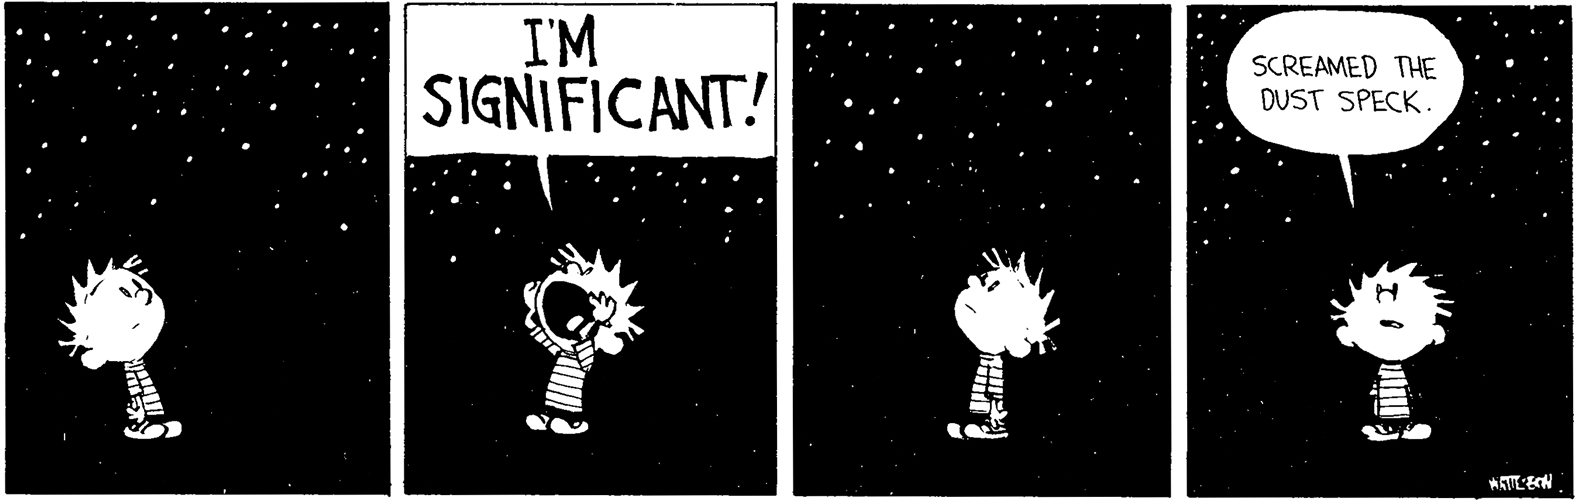
\includegraphics[width=\textwidth]{Figures/calvin_1}
%     \caption*{\centering \textit{Calvin and Hobbes} by Bill Watterson (1993). Reproduced with permission.} 
% \end{figure}

\begin{figure}
	\centering
	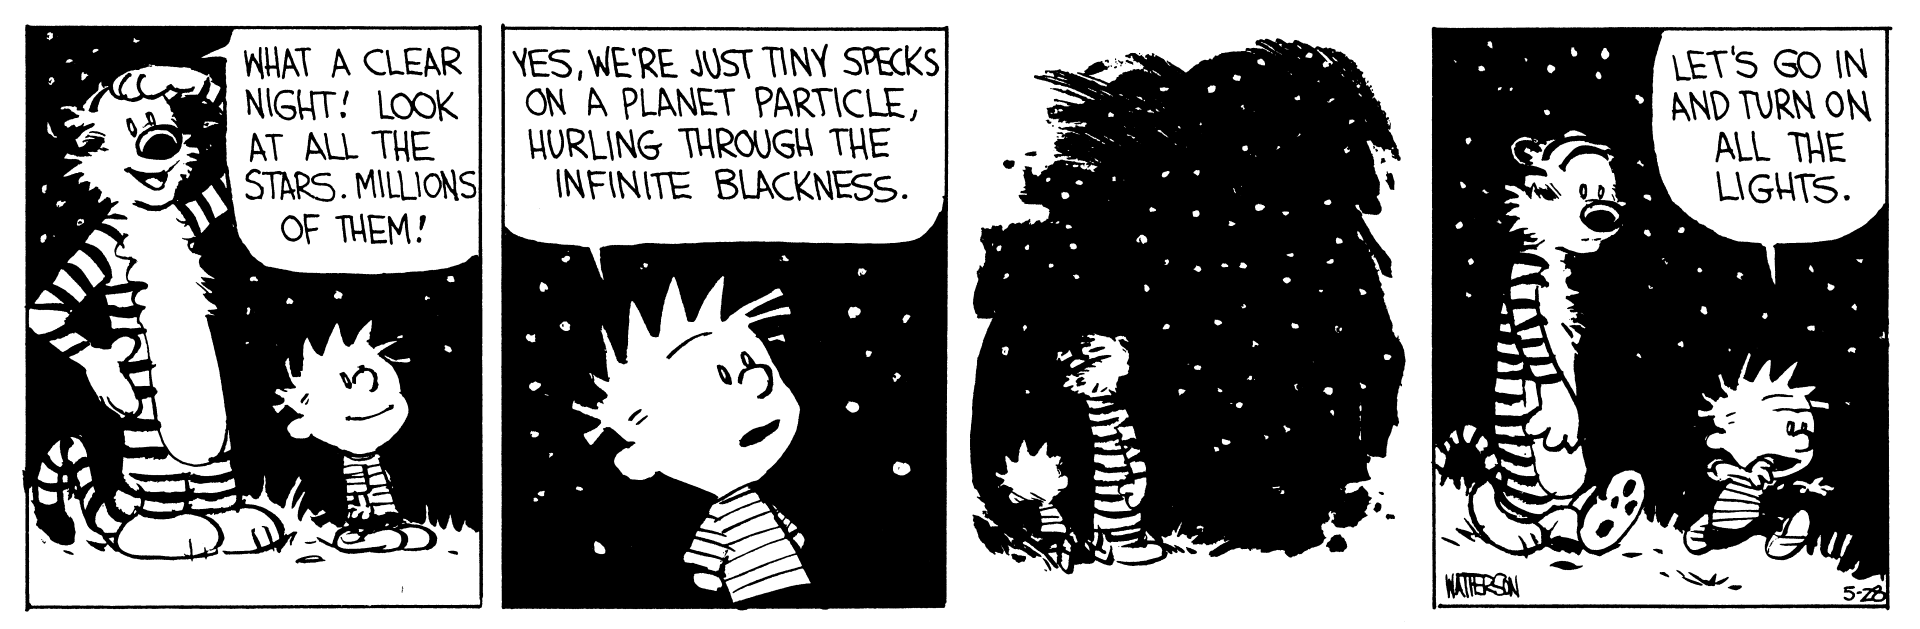
\includegraphics[width=\textwidth]{Figures/calvin_2}
    \caption*{\centering \textit{Calvin and Hobbes} by Bill Watterson (1988). Reproduced with permission.} 
\end{figure}               % Quotation page



%----------------------------------------------------------------------------------------
%	THESIS CONTENT - CHAPTERS
%----------------------------------------------------------------------------------------

\pagestyle{thesis} % Return the page headers back to the "thesis" style

% Include the chapters of the thesis as separate files from the Chapters folder
% Uncomment the lines as you write the chapters
\chapter{Introduction}
\label{chapt: intro}

`A pulsar', so goes the traditional paper opening, `is a highly magnetised, rapidly rotating neutron star'. The first pulsar discovered was CP~1919+21 (PSR~B1919+21 or PSR~J1921+2153 in modern nomenclature) by \citet{HBP+1968} in Cambridge on 28 November 1967. Appearing as a series of regularly spaced peaks in radio observations, the signals were quickly associated with emission from the then-theoretical neutron stars \citep{BZxx1934}; extremely compact stellar remnants produced by supernovae, with masses of around 1.4 solar masses (M$_\odot$) and radii of approximately 10~km \citep[e.g.][]{PulsarAstronomy}. These properties place neutron stars among the densest objects in the universe with an average density of $\sim$6.7$\times10^{17}$~kg~m$^{-3}$, around three times the density of nuclear matter \citep[$2.3\times10^{17}$~kg~m$^{-3}$; e.g.][]{Lxxx2001}. This density makes the rotation of neutron stars extremely stable, and gives them strong surface gravitational fields. Neutron stars also have incredibly powerful magnetic fields; about $10^{12}$~gauss at the stellar surface \citep{Gxxx1968}.

Pulsars -- `PULSating stARS' -- appear in radio-frequency time series observations as a series of regularly separated peaks. Their radio emission is believed to be produced from around their magnetic axis, which is not necessarily aligned with their rotation axis. As the star rotates, the radio beam sweeps around the sky creating an effect that is comparable to a `cosmic lighthouse'. The inclined magnetic axis causes the pulsar to lose energy through the emission of magnetic dipole radiation, leading to the prediction of a gradual decrease in their rotation rates \citep{Pxxx1968}\footnote{In this early model, \citet{Pxxx1968} only considered magnetic dipole radiation in free space; the presence of the dense magnetosphere also contributes to the spin-down of pulsars through the outflow of particles along the open magnetic field lines.}. This was first confirmed by the spin-down of the Crab pulsar (PSR~B0531+21), whose period was observed to increase by 36~ns per day \citep{RCxx1969_crab}.

The presence of a strong magnetic field surrounding a dense, superconducting star causes a pulsar to act as a homopolar or `Faraday disc' generator, in which an enormous potential difference is generated between the poles and the equator. For a pulsar where the magnetic and rotation axes are aligned (an `aligned rotator'), \citet{GJxx1969} calculated that the induced electric fields would lead to streams of electrons being emitted from the poles, and bunches of ions being produced from the equator. These particles form a dense plasma magnetosphere around the star, in which the charged particles co-rotate with the pulsar up until the `light cylinder' radius, the distance at which their velocities would have to exceed the speed of light to maintain co-rotation. Later analysis showed that the surface of a neutron star is not hot enough to sustain an outflow of positively charged ions. \citet{RSxx1975} instead proposed a model in which electron-positron pairs are produced within a `polar gap' close to the surface of the magnetic poles, in which the enormous electric fields are not screened by plasma. The positrons escape from the star along the open magnetic field lines, and to close the homopolar generator circuit the electrons return to the surface of the pulsar.

Radio emission produced by a pulsar is believed to originate from these ultra-relativistic particles streaming from the magnetic poles, at a certain height above the surface of the star. The structure of the emission region is not yet fully understood, and a successful model must explain both the variability of individual pulses, and the stability of the profile integrated over long periods. The rotating carousel model proposed by \citet{RSxx1975} can explain the time-dependent periodic drift seen in the individual pulses of some pulsars.  % OLD: In the model proposed by \citet{RSxx1975}, the rotating carousel model can explain the time-dependent periodic drift seen in the individual pulses of some pulsars. 

A key aspect of pulsar radio emission is its polarisation. The long-established model which aims to explain the change in linear polarisation angle with pulse phase is the Rotating Vector Model \citep[RVM;][]{RCxx1969}. This is a purely geometric model that suggests that the angle of polarisation depends only on the rotational phase of the pulsar and the observing geometry. However, deviations from this model are commonly seen, for example in the form of discontinuous polarisation angle jumps. These are thought to originate from two modes of emission which are orthogonally polarised, with the observed transition occurring when the dominating mode changes.

This introductory chapter is designed to provide an overview of the properties of radio pulsars, and to introduce the key models and concepts on which the rest of this thesis is based. Section~\ref{sec: intro - general intro} presents the observable spin parameters of pulsars and explains how these may be used to derive other properties. The population is then introduced, and different classes are highlighted in Sec.~\ref{sec: intro - general intro - pulsar population}. Section~\ref{sec: intro - emission models} gives a basic overview of how the radio emission is produced. Pulsar polarisation and models are introduced in Sec.~\ref{sec: intro - emission models - polarisation}, and the variability of single pulses is described in Sec.~\ref{sec: intro - emission models - single pulse phenomena}. Section~\ref{sec: intro - observation processing} describes polarisation and flux calibration of pulsar data and Sec.~\ref{sec: intro - observation processing - ISM effects} explains some of the effects of the interstellar medium on propagating radiation. Finally, Sec.~\ref{sec: intro - thesis outline} gives an outline of the following chapters and results of this thesis.












\section{Properties of radio pulsars}
\label{sec: intro - general intro}

This section introduces the basic properties of radio pulsars which can be measured from their radio pulses. A simple schematic view of the geometry of a pulsar is shown in Fig.~\ref{fig: intro - basic geometry}. The magnetic field at the altitude above the surface of the star where the radio emission is produced is thought to be dominated by the dipole moment\footnote{Higher magnetic moments may also be present and could even dominate near the stellar surface, especially in millisecond pulsars \citep[e.g.][]{GMGx2003, BWH+2019}.}. The two main parameters that describe the viewing geometry are the angles $\alpha$ and $\beta$. The magnetic inclination angle $\alpha$ is the angle between the rotation and magnetic axes, and $\beta$ is the impact angle between the magnetic axis and the observer's line of sight (LOS) as the pulsar rotates. 
\begin{figure}
    \begin{center}
        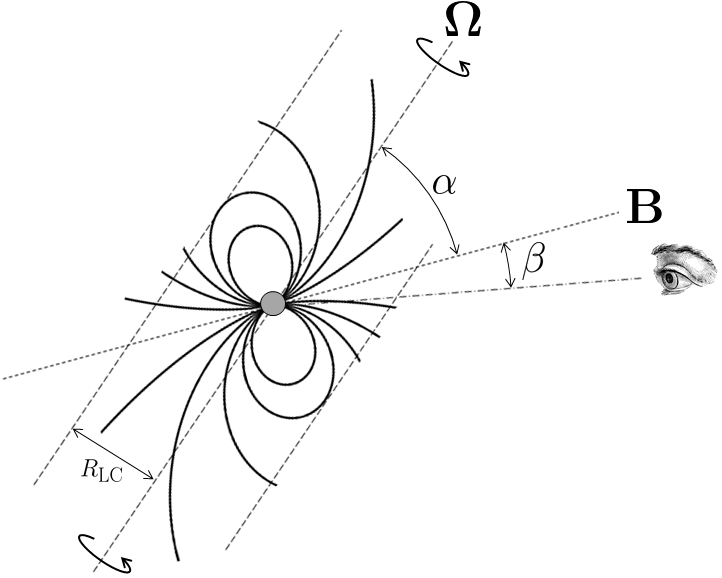
\includegraphics[width=0.75\textwidth]{Figures/Introduction/pulsar_geometry}
        \caption[The basic geometry of a radio pulsar]{The geometry of a pulsar with a dipolar magnetic field ($\mathbf{B}$) inclined at an angle $\alpha$ to the rotation axis ($\mathbf{\Omega}$). The observer's line of sight makes an angle $\beta$ to the magnetic axis. The light cylinder radius $R_\mathrm{LC}$ is the distance at which an object corotating with the pulsar would have a speed equal to the speed of light, $c$.}
        \label{fig: intro - basic geometry}
    \end{center}
\end{figure}
Although the magnetosphere co-rotates with the star, co-rotation can only be sustained up to the distance at which a particle would have to move at the speed of light. This defines the `light cylinder', which is at a radius $R_\mathrm{LC} = cP/2\pi$, where $c$ is the speed of light and $P$ is the pulsar's rotation period. If a magnetic field line remains within $R_\mathrm{LC}$ it reconnects to the pulsar and is a `closed' field line, whereas those that cross the light cylinder are `open' field lines and particles with trajectories bound to these can escape the pulsar. At this boundary, the last set of field lines which cross $R_\mathrm{LC}$ are referred to as the `last open field lines', and these form the boundary around the `open-field-line region' which contains all field lines which do not close within $R_\mathrm{LC}$

As illustrated in Fig.~\ref{fig: intro - emission cone}, the radio emission is thought to originate from within a cone around the magnetic axis, which is bound by the tangents to the last open field lines at the emission height $h_\mathrm{em}$.  
\begin{figure}
    \begin{center}
        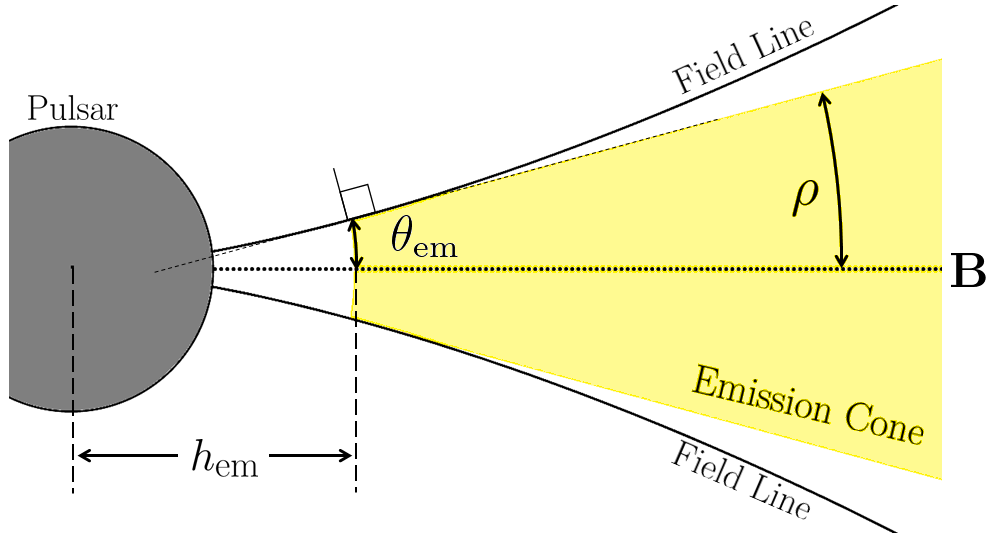
\includegraphics[width=0.75\textwidth]{Figures/Introduction/cone}
        \caption[The geometry of the emission cone]{The cone of emission of half opening angle $\rho$ surrounding the magnetic axis, $\mathbf{B}$. The cone is delimited by tangents to the last open field lines at the emission height $h_\mathrm{em}$. The open-field-line region has an angular radius of $\theta_\mathrm{em}$ (measured from the centre of the star).}
        \label{fig: intro - emission cone}
    \end{center}
\end{figure}
The last open field lines define an area on the surface of the star known as the `polar cap'. At a height $h_\mathrm{em}$, the area bound by these field lines has an angular radius of 
\begin{equation}
    \label{eq: intro - polar cap radius}
	\theta_\mathrm{em} = \arcsin\bigg(\sqrt{\frac{2\pi h_\mathrm{em}}{cP}}\bigg)
\end{equation} 
when measured from the centre of the star. The half opening angle of the emission cone formed by tangents to the last open field lines is
\begin{equation}
    \label{eq: intro - cone half opening angle}
	\rho = \theta_\mathrm{em} + \arctan\bigg(\frac{1}{2}\tan\theta_\mathrm{em}\bigg).
\end{equation} 
These relations were derived assuming a dipolar magnetic field structure \citep[see][]{PulsarAstronomy}. The size of the emission cone depends on $P$ -- generally speaking, slower pulsars have narrower emission cones. This is discussed further for the slowest-known pulsar PSR~J0250+5854 ($P = 23.5$~s) in Chapter~\ref{chapt: J0250}.








\subsection{Pulsar spin parameters and derived quantities}
\label{sec: intro - general intro - spin parameters}

The two fundamental directly measurable properties of a pulsar are its rotational period, $P$, and its spin-down rate, $\dot{P}$. From these two quantities, many other properties of the pulsar can be estimated. The spin-down rate of the star $\dot{P} = \mathrm{d}P/\mathrm{d}t > 0$ implies that it is losing energy. The rate of loss of rotational kinetic energy is
\begin{equation}
    \label{eq: intro - Edot}
    \dot{E} = -I\Omega\dot{\Omega} = 4\pi^2I\frac{\dot{P}}{P^3},
\end{equation}
where $\Omega = 2\pi/P$ is the rotational angular frequency and $I$ is the moment of inertia of the star. Canonically in pulsar astronomy, $I$ is taken to be the moment of inertia of a solid sphere with mass $M=$1.4~M$_\odot$ and $R=10$~km. This gives $I=2MR^2/5\simeq 10^{45}$~g~cm$^2$. This means that the total power output from a pulsar, known as its spin-down luminosity, is
\begin{equation}
    \label{eq: intro - Edot canonical}
    \dot{E} \approx 3.95\times10^{31} \bigg(\frac{\dot{P}}{10^{-15}}\bigg) \bigg(\frac{P}{\mathrm{s}}\bigg)^{-3} \mathrm{erg\ s}^{-1}.
\end{equation}


\subsubsection{Characteristic age}
\label{sec: intro - general intro - spin parameters - characteristic age}

The dominant magnetic field component of a pulsar is generally assumed to be dipolar \citep[][]{Pxxx1968}, where the magnetic axis is inclined at some angle $\alpha$ to the rotation axis. In classical electrodynamics, a rotating magnetic dipole in a vacuum loses energy through the emission of electromagnetic radiation. This occurs at a rate of 
\begin{equation}
    \label{eq: intro - dipole Edot}
    \dot{E}_\mathrm{dipole} = \frac{2\Omega^4|\mathbf{m}|^2\sin^2\alpha}{3c^3},
\end{equation}
where $\mathbf{m}$ is the magnetic dipole moment, and $c$ is the speed of light \citep[see for example][]{Jxxx1962}. If all energy loss from the pulsar is due to magnetic dipole radiation, then $\dot{E}_\mathrm{dipole} = \dot{E}$ (see Eq.~\eqref{eq: intro - Edot}), and the rotation frequency evolves with time according to
\begin{equation}
    \label{eq: intro - rotation frequency evolution}
    \dot{\Omega} = -\bigg( \frac{2|\mathbf{m}|^2\sin^2\alpha}{3Ic^3}\bigg)\Omega^3.
\end{equation} 
Equation~\eqref{eq: intro - rotation frequency evolution} can be generalised as the power law relation
\begin{equation}
    \label{eq: intro - period power law}
    \dot{P} = kP^{2-n},
\end{equation}
where $k$ is often assumed to be constant, and $n$ is known as the braking index. If magnetic dipole radiation dominates, $n=3$ as in Eq.~\eqref{eq: intro - rotation frequency evolution}. The actual braking index follows from precise pulsar timing, which allows the rate of change of $\dot{P}$, $\ddot{P}$, to be measured \citep[e.g.][]{Lxxx2020}. A broad range of braking indices have been found in the population \citep[e.g.][]{HLK+2004,HLKx2010}, pointing to complex additional physics playing a role in the spin-down of pulsars.

If $k$ and $n\neq 1$ are assumed to remain constant over the lifetime of a pulsar, Eq.~\eqref{eq: intro - period power law} can be integrated to calculate the age of the pulsar,
\begin{equation}
    \label{eq: intro - pulsar age}
    T = \frac{P}{(n-1)\dot{P}}\bigg[ 1 - \bigg(\frac{P_0}{P}\bigg)^{n-1} \bigg],
\end{equation}
where $P_0$ is the period of the pulsar at its birth. Finally, under the assumption of pure magnetic dipole radiation ($n=3$) and $P_0 \ll P$, the characteristic age of the pulsar,
\begin{equation}
    \label{eq: intro - characteristic age}
    \tau_c = \frac{P}{2\dot{P}},
\end{equation}
is obtained. Due to the assumptions involved, this does not necessarily give an accurate calculation of the true age of a given pulsar. However, it serves as a useful indicator of age that can be readily obtained from the observable properties and is widely quoted in the literature.


\subsubsection{Surface magnetic field strength}
\label{sec: intro - general intro - spin parameters - surface B field}

The surface magnetic field strength of a pulsar may also be obtained from its spin parameters, again under the assumption that the source of energy loss is purely magnetic dipole radiation. In this case, the magnetic moment is related to the magnetic field strength at the equator according to $B(r) = 10^4 \mu_0 |\mathbf{m}|/4\pi r^3$~gauss, where $\mu_0$ is the vacuum permeability \citep[e.g.][]{Jxxx1962}. Substituting this into Eq.~\eqref{eq: intro - rotation frequency evolution}, the magnetic field strength at the surface of the star ($r=R$) is given by
\begin{equation}
    \label{eq: intro - pulsar field strength}
    B_\mathrm{S} = \sqrt{\frac{3c^3}{8\pi^2}\frac{I}{R^6 \sin^2\alpha}P\dot{P}}.
\end{equation}
Once again, taking the canonical values $I=10^{45}$~g~cm$^2$ and $R=10$~km, and assuming $\alpha = 90\degr$, we find
\begin{equation}
    \label{eq: intro - characteristic B field}
    B_\mathrm{S} = 3.2\times 10^{19} \sqrt{P\dot{P}} \mathrm{\ gauss}.
\end{equation}
As for the characteristic age, the estimated magnetic field strength depends on multiple assumptions and so should be treated only as an order-of-magnitude estimate. Furthermore, Eq.~\eqref{eq: intro - characteristic B field} describes the field at the magnetic equator of the star -- the field strength at the magnetic poles ought to be twice as large \citep{STxx1983,UMxx1995}.




















\subsection{The pulsar population}
\label{sec: intro - general intro - pulsar population}

There are a variety of different types of pulsar in the population, all with slightly different properties. To date, the fastest spinning pulsar known is PSR~J1748-2446ad with $P=1.4$~ms \citep{HRS+2006}, and the slowest is PSR~J0250+5854 with $P=23.5$~s \citep[][see Chapter~\ref{chapt: J0250}]{TBC+2018}. A very useful way to visualise the population is to plot them on the $P$-$\dot{P}$ diagram, such as in Fig.~\ref{fig: intro - ppdot diagram}. This figure shows how pulsars fall into groups based on their periods and spin-down rates; it also shows lines of constant characteristic age and magnetic field, as defined in Sec.~\ref{sec: intro - general intro - spin parameters}. The four pulsars studied in detail in this thesis are also highlighted in orange: PSR~B0031$-$07 is shown by the star, PSR~J1926$-$0652 by the pentagon, PSR~J1518+4904 by the diamond, and J0250+5854 by the triangle.
\begin{figure}
    \begin{center}
        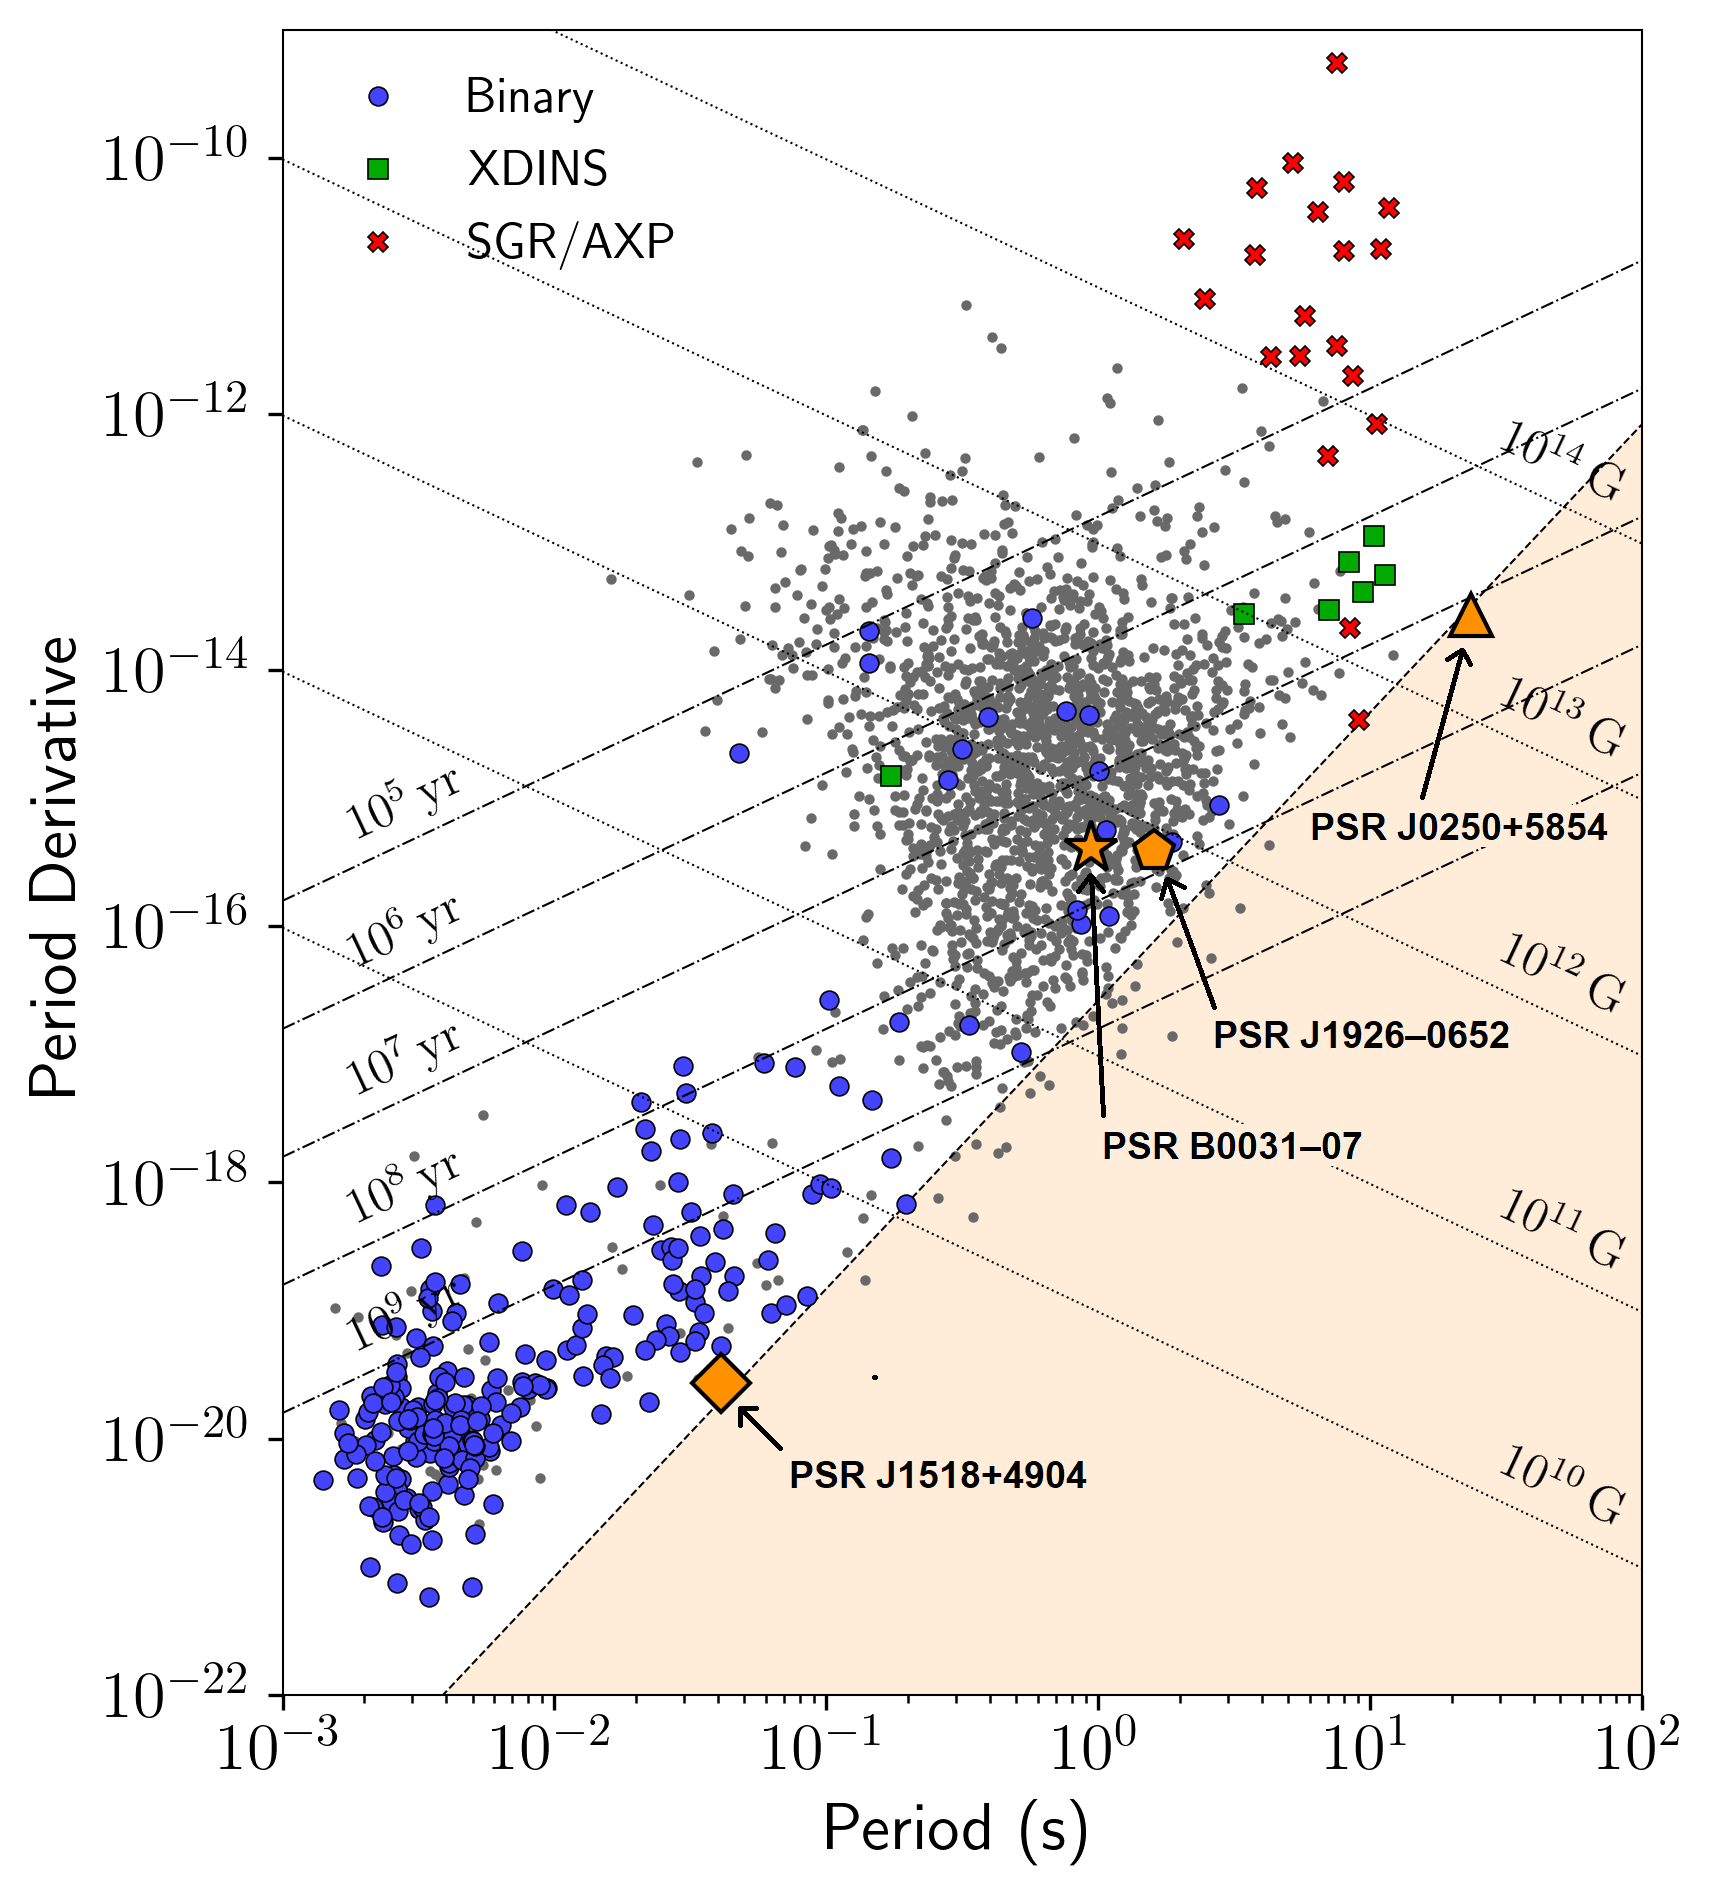
\includegraphics[width=1.0\textwidth]{Figures/Introduction/ppdot_diagram_labelled}
        \caption[The period and period derivative diagram]{The $P$-$\dot{P}$ diagram, showing the pulsar population with parameters retrieved from the Australia Telescope National Facility pulsar database \citep{ATNFcatalogue} in May 2021. The blue circles indicate pulsars in a binary system. The red crosses show the magnetars, while the green squares highlight XDINSs. The four different orange shapes indicate PSRs~B0031$-$07 (star), J1926$-$0652 (pentagon), J1518+4904 (diamond), and J0250+5854 (triangle). The Python module \texttt{psrqpy} published by \citet{Pxxx2018} was used to create the diagram.}
        \label{fig: intro - ppdot diagram}
    \end{center}
\end{figure}
From the $P$-$\dot{P}$ diagram, groupings of pulsars can be identified, as discussed next.


\subsubsection{`Normal' pulsars}
\label{sec: intro - general intro - pulsar population - normal}

The majority of pulsars are found in the middle of the $P$-$\dot{P}$ diagram, and are often referred to as the `normal' pulsars. They typically have periods of around 0.5~s and spin-down rates of ${\sim}10^{-15}$~s~s$^{-1}$, giving them estimated magnetic fields of $B_\mathrm{S} \sim 10^{11}-10^{13}$~gauss. Pulsars of this type are thought to be born in the upper left of the $P$-$\dot{P}$ diagram with relatively short periods and high spin-down rates. As they age, they migrate towards the bottom right following a contour of constant $B_\mathrm{S}$ if dipole radiation is the only rotational energy loss mechanism -- although more complex evolutionary tracks have been theorised (see e.g. \citealt{JKxx2017} and references therein) -- until they cross the `death line', which is the theoretical limit below which it is believed that radio emission ceases to be produced. This is not a sharp limit however, and is sometimes referred to as more of a `death valley'. The death line in Fig.~\ref{fig: intro - ppdot diagram} is the boundary of the pale yellow shaded region, and the model shown here is given by Eq.~6 of \citet{ZHMx2000}. It can be seen that a number of pulsars, including the slow pulsar PSR~J0250+5854 (see Chapter~\ref{chapt: J0250}), lie beyond this limit -- this highlights that this subject is a topic of much debate, and multiple different death line models have been proposed \citep[e.g.][]{CRxx1993,ZHMx2000, FKxx2006, JKxx2017, MBMA2020}.


\subsubsection{Millisecond pulsars}
\label{sec: intro - general intro - pulsar population - MSPs}

Towards the lower left of the $P$-$\dot{P}$ diagram are the millisecond pulsars, or MSPs. These are much older pulsars with much lower spin-down rates of ${\sim}10^{-20}$~s~s$^{-1}$. The majority of MSPs are in binary systems (indicated by the blue points in Fig.~\ref{fig: intro - ppdot diagram}), and are `recycled pulsars'. These are objects which have at some point in the past undergone mass accretion from their binary companion; this process transfers angular momentum to the pulsar, causing it to spin-up to very short periods, and it can also suppress their magnetic fields \citep{BKxx1974, SMSN1989}. Before spin-up these were older, normal pulsars, decaying in luminosity as they lose energy -- the increase in rotational energy through accretion rejuvenates them causing them to once again emit radio waves, hence they are referred to as `recycled'. Their short periods make MSPs ideal precision timing sources for the detection of gravitational waves, through pulsar timing arrays \citep[e.g][]{FBxx1990,MHB+2013}. At present only one binary MSP is known to have another pulsar as companion -- the `double pulsar', PSRs~J0737–3039A ($P=22.7$~ms) and J0737–3039B ($P=2.8$~s) discovered by \citet{BDP+2003}.
% Recycled pulsars are objects which have at some point in the past undergone mass accretion from their binary companion; this causes them to spin-up to a typical rotational speed of hundreds of rotations per second \citep[e.g.][]{PulsarAstronomy}. Before spin-up these were older, normal pulsars, decaying in luminosity as they lose energy -- the increase in rotational energy through accretion rejuvenates them causing them to once again emit radio waves. An overview of the pulsar population is given in Sec.~\ref{sec: intro - general intro - pulsar population}.
\subsubsection{Magnetars and more}
\label{sec: intro - general intro - pulsar population - magnetars etc}

The most energetic pulsars can be found up in the top right of the $P$-$\dot{P}$ diagram. These include the magnetars (shown by the red crosses in Fig.~\ref{fig: intro - ppdot diagram}), given their name due to their extremely strong magnetic fields ($>10^{14}$~G). As of November 2020 there are 24 confirmed magnetars and 6 candidate sources\footnote{See the McGill Magnetar Catalogue; \url{http://www.physics.mcgill.ca/~pulsar/magnetar/main.html}} \citep{OKxx2014}. Magnetars produce mostly high-energy emission, for example X-rays and $\gamma$-rays, and include the soft gamma repeaters (SGRs) which produce bursts of high-energy emission at irregular intervals, and anomalous X-ray pulsars (AXPs) whose emission is believed to be produced by the decay of their magnetic fields \citep{TDxx1995, TDxx1996, Mxxx2008}. Thus, they are non-rotation-powered. While most magnetars are only detected via their high-energy emission, radio pulses have been detected from five: 1E~1547.0$-$5408 \citep{CRHR2007a}, PSR~J1622$-$4950 \citep{LBB+2010}, PSR~J1745$-$2900 \citep{EFK+2013}, XTE~J1810$-$197 \citep{CRH+2006}, and Swift~J1818$-$1607 \citep{ERB+2020, LSJB2020}.

One of the sources studied in this thesis (PSR~J0250+5854, the orange triangle in Fig.~\ref{fig: intro - ppdot diagram}, see Chapter~\ref{chapt: J0250}) lies close to a cluster of objects known as X-ray Dim Isolated Neutron Stars (XDINSs; indicated by the green squares). There are seven of these objects (informally known as `The Magnificent Seven', e.g. \citealt{Hxxx2007}) which are characterised by pulsed X-ray emission with a soft, blackbody-like spectrum and periods between 3.4 and 11.3 seconds. Although they are similar to and potentially evolved from magnetars \citep{VRP+2013}, no radio emission from XDINSs has yet been detected \citep{Jxxx2003, KKM+2003, KML+2009}.









\section{Radio emission and models}
\label{sec: intro - emission models}

% Briefly summarise the emission models, and stress that this thesis is particularly interested in the single pulse and polarisation properties
Based on the work by \citet{Gxxx1968}, who first suggested that pulsars are magnetised, rotating neutron stars, \citet{GJxx1969} investigated the simplest case of a pulsar in which the magnetic dipole axis is aligned with the rotation axis. They concluded that, despite the intense surface gravitational field, the pulsar must possess a dense magnetosphere which co-rotates with the star up until the light cylinder radius (see Fig.~\ref{fig: intro - basic geometry}). In the corotating plasma, $\mathbf{E}\cdot\mathbf{B} = 0$ and the net magnetospheric charge density is $7\times10^4 B_z P^{-1}$ electronic charges per cubic metre, where $B_z$ is the component of the magnetic field in the direction of the rotation axis ($B_z = \mathbf{B}\cdot\mathbf{\hat{\Omega}}$, measured in gauss) -- this is known as the Goldreich-Julian density, $\rho_\mathrm{GJ}$, and is the net charge density required to screen the rotation-induced electric fields \citep{GJxx1969}.

Magnetic field lines which exit the light cylinder do not re-enter, instead closing in a boundary zone layer near the shell of the supernova remnant. Charged particles can escape the pulsar along these open field lines, forming the wind zone surrounding the light cylinder up to a distance of about one tenth of the radius of the supernova remnant shell surrounding the star. Here, unlike closer to the star, the currents due to the charged particles are the main source of the magnetic field. It is the motion of the charged particles along the open field lines within the light cylinder which gives rise to the beamed electromagnetic radiation from the magnetic poles.

Further analysis by \citet{RSxx1975} led to one of the best-known models of pulsar radio emission. % Nuclei -- mostly iron -- in the crust of neutron stars form a tightly bound condensed state due to the strong magnetic field: both theory and observations have shown that the surface of a pulsar is not hot enough to sustain an ejection of positive ions to balance the outflow of electrons along the open field lines. This is true for all but the youngest (most energetic) and hottest of pulsars, for example the Crab \citep{RSxx1975}.
Like \citet{GJxx1969}, \citet{RSxx1975} considered an aligned rotator; one in which the magnetic moment is antiparallel to the spin angular momentum vector (in the community this is sometimes referred to simply as a pulsar, whereas the opposite case where the magnetic and spin vectors point in the same direction is called an `anti-pulsar'). By assuming that ejected electrons do not return to the star by the open field lines, they concluded the existence of a `polar gap' in the magnetosphere, reaching from the stellar surface to an altitude of around 100~metres. Within the gap, $\mathbf{E}\cdot\mathbf{B} \neq 0$, although it essentially vanishes elsewhere -- this leads to a large potential difference across the gap of around $10^{12}$~V. On microsecond timescales the gap breaks down by forming electron-positron pairs; the positrons move outward along the open field lines and the electrons flow back to the surface to close the homopolar generator circuit.

Moreover, in the related \citet{Sxxx1971} model electron-positron pairs are produced from the energetic curvature radiation photons from accelerating charges travelling along the curved field lines. The charge density along the open field lines was taken to be much less than required for co-rotation \citep{GJxx1969}, essentially treating the open-field-line region as empty of corotating magnetosphere. In this scenario \citet{RSxx1975} argue that the potential difference in the gap would be much greater than the space charge effects in the magnetosphere associated with bringing the electrons to relativistic speed. If the gap is not present and acceleration of the electrons is purely due to space charges, for a pulsar with $P\approx1$~s there would be a potential drop of less than $10^{10}$~V above the surface \citep{Mxxx1974}, far too low for further pair production by curvature radiation. \citet{RSxx1975} therefore conclude that the polar gap is a crucial part of pulsar radiation and that the magnetosphere within the open field lines also plays an important role, an idea that has been developed in more recent years \citep[e.g.][]{CRxx1980,ZQHx1997,Txxx2010, SMGx2015}.

\citet{RSxx1975} also predicted that the breakdown of the polar gap occurs through discrete, localised `sparks' which inject positron beams into the magnetosphere beyond the gap. There, they produce the plasma and bunching that ultimately leads to the production of coherent radio emission. As discussed in Sec.~\ref{sec: intro - emission models - single pulse phenomena - carousel model}, the location of the sparks on the polar cap determines the pattern of sub-beams which rotate in a carousel-like structure, which can explain the existence of so-called drifting subpulses.



\subsection{Polarisation properties}
\label{sec: intro - emission models - polarisation}

Radio waves are a form of electromagnetic (EM) radiation, which in a vacuum is a transverse wave. The magnetic and electric field components are perpendicular to one another, both being orthogonal to the direction of propagation of the wave. The orientation of the electric field vector determines the polarisation state of the EM wave.

A common representation of polarisation is by the use of Stokes' parameters -- $I$, $Q$, $U$, and $V$ -- which fully describe the average polarisation state of a beam of light. The total intensity of the beam is given by $I$, which for a fully polarised beam is the sum in quadrature of the other components:
\begin{equation}
    \label{eq: stokes parameters quadrature}
    I^2 = Q^2 + U^2 + V^2.   
\end{equation}
The Stokes parameters are formed by considering the combination of the two (Cartesian) components of the electric field of the EM wave, $E_x$ and $E_y$. By time-averaging the $x$ and $y$ components of a crossed dipole common in the `linear feed' of many receivers, the Stokes parameters can be written
\begin{align}
    I = \langle E_x^2 \rangle + \langle E_y^2 \rangle, \label{eq: intro - stokes I linear}\\
    Q = \langle E_x^2 \rangle - \langle E_y^2 \rangle, \label{eq: intro - stokes Q linear}\\
    U = 2\langle E_x\rangle \langle E_y\rangle \cos\phi, \label{eq: intro - stokes U linear}\\
    V = 2\langle E_x\rangle \langle E_y \rangle \sin\phi, \label{eq: intro - stokes V linear}
\end{align}  
where $\phi$ is the relative phase between $E_x$ and $E_y$ \citep{Handbook}.

Linear polarisation is represented by the orthogonal components $Q$ and $U$, where the total linearly polarised intensity of a wave is given by $L = \sqrt{Q^2 + U^2}$. The circularly polarised intensity $V$ can be either positive or negative depending on the handedness of the circular polarisation, and occurs when there is a phase delay between the $x$- and $y$-components of the electric field vector. The polarisation vector $\mathbf{p}$, expressed in Cartesian coordinates as $(Q,U,V)$, has a magnitude
\begin{equation}
    \label{eq: polarisation vector magnitude}
    |\mathbf{p}| = \sqrt{Q^2 + U^2 + V^2}
\end{equation}
and can be smaller than $I$ for partially polarised radiation.

\begin{figure}
    \begin{center}
        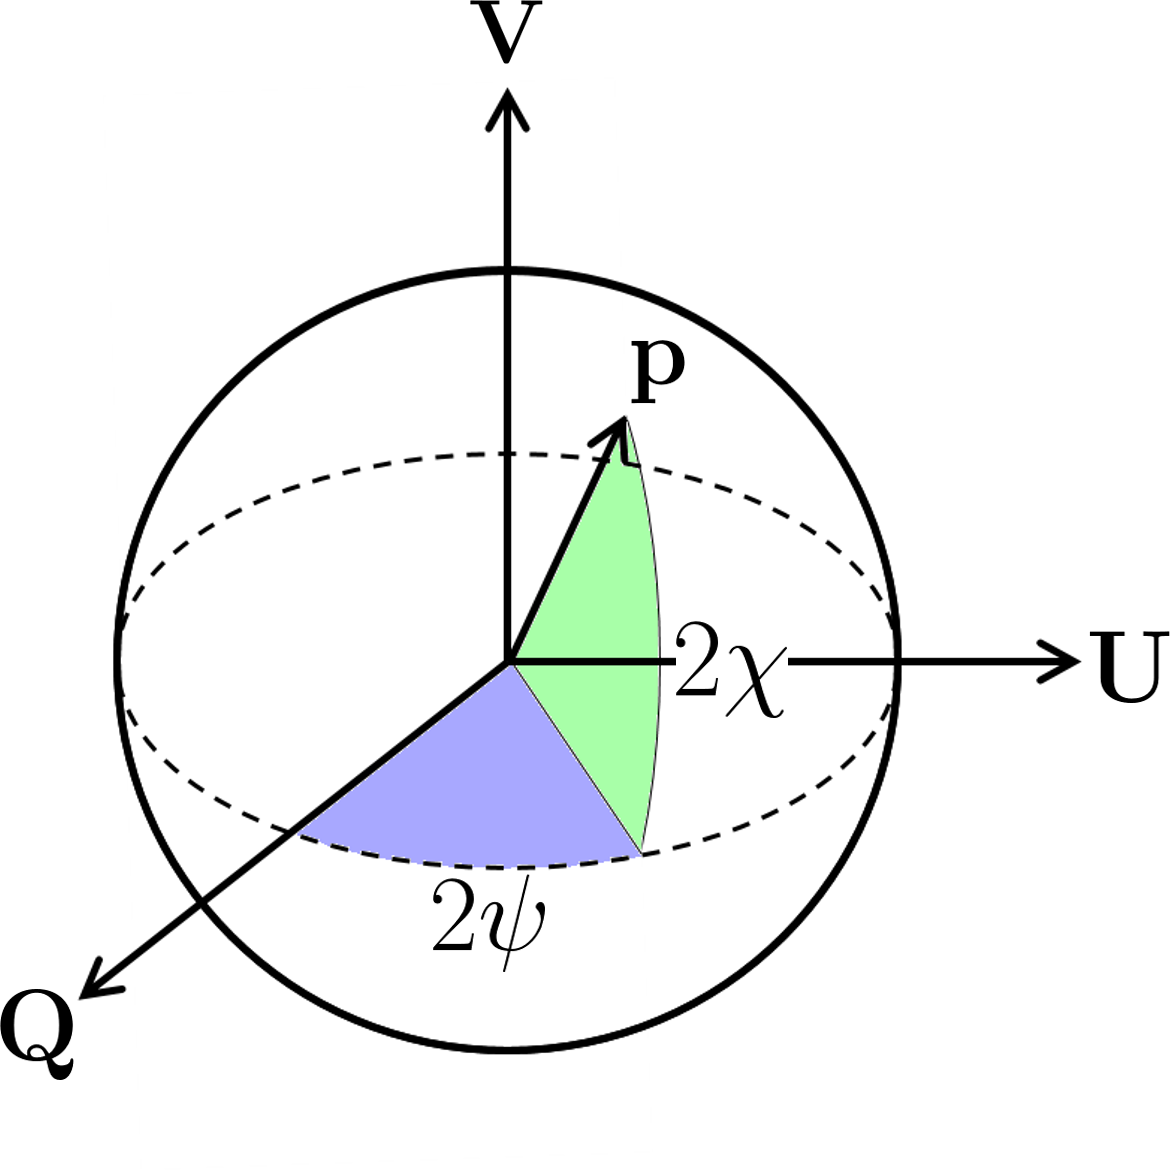
\includegraphics[width=0.4\textwidth]{Figures/Introduction/poincare_sphere}
        \caption[Polarisation vector on the Poincar\'e sphere]{A representation of the polarisation vector $\mathbf{p}$ on the Poincar\'e sphere. The mutually orthogonal basis vectors are formed by Stokes parameters $Q$, $U$, and $V$. The position angle is given by $\psi$, whilst the ellipticity angle is $\chi$. If a wave is purely linearly polarised, then $\mathbf{p}$ will lie in the $(Q,U)$ plane.}
        \label{fig: intro - Poincare sphere}
    \end{center}
\end{figure}
The polarisation vector is commonly depicted by use of the Poincar\'e sphere, as illustrated in Fig.~\ref{fig: intro - Poincare sphere}. This graphically represents the orientation of the polarisation, and the polarised intensity corresponds to the radius of a sphere. The space is defined by three orthogonal basis vectors: $\hat{\mathbf{Q}}$, $\hat{\mathbf{U}}$, and $\hat{\mathbf{V}}$. Figure~\ref{fig: intro - Poincare sphere} also introduces the position angle (PA) $\psi$ of the linear polarisation and the ellipticity angle $\chi$. As indicated in the figure, the PA is given by
\begin{equation}
    \label{eq: position angle definition}
    \psi = \frac{1}{2}\arctan\bigg(\frac{U}{Q}\bigg),
\end{equation}
and the ellipticity angle is 
\begin{equation}
    \label{eq: ellipticity angle definition}
    \chi = \frac{1}{2}\arctan\bigg(\frac{V}{\sqrt{Q^2 + U^2}}\bigg) = \frac{1}{2}\arctan\bigg(\frac{V}{L}\bigg).
\end{equation}
The double angles $2\psi$ and $2\chi$ in Fig.~\ref{fig: intro - Poincare sphere} highlight the fact that the angles of polarisation are periodic on $\pi$ rather than $2\pi$ for phase. The PA is of particular interest in pulsar astronomy as it varies as function of pulse longitude, describing a characteristic S-shaped curve, which can be interpreted by the Rotating Vector Model as will be described next.


\subsubsection{Linear polarisation and the Rotating Vector Model}
\label{sec: intro - emission models - polarisation - RVM}

% Describe expectations (strong linear polarisation)
The emission of radio pulsars, especially the younger ones, typically exhibits a high degree of polarisation, especially linear polarisation \citep[e.g.][]{QMLG1995, CMKx2001}. The position angle (PA) of the linear polarisation is observed to depend on pulse longitude, and hence is often associated with the changing orientation of the magnetic field lines with respect to the observer's line of sight. The shape of the PA curve is usually simple, S-shaped, and monotonic, even when the total intensity profile has multiple components \citep{WCL+1999}. This implies that the orientation of the linear polarisation is independent of the intensity of different sources of emission, affected only by the location of source within the emission region. Figure~\ref{fig: intro - vela polarisation} shows the polarised profile and smooth PA curve of the Vela pulsar (PSR~B0833$-$45).
\begin{figure}
    \begin{center}
        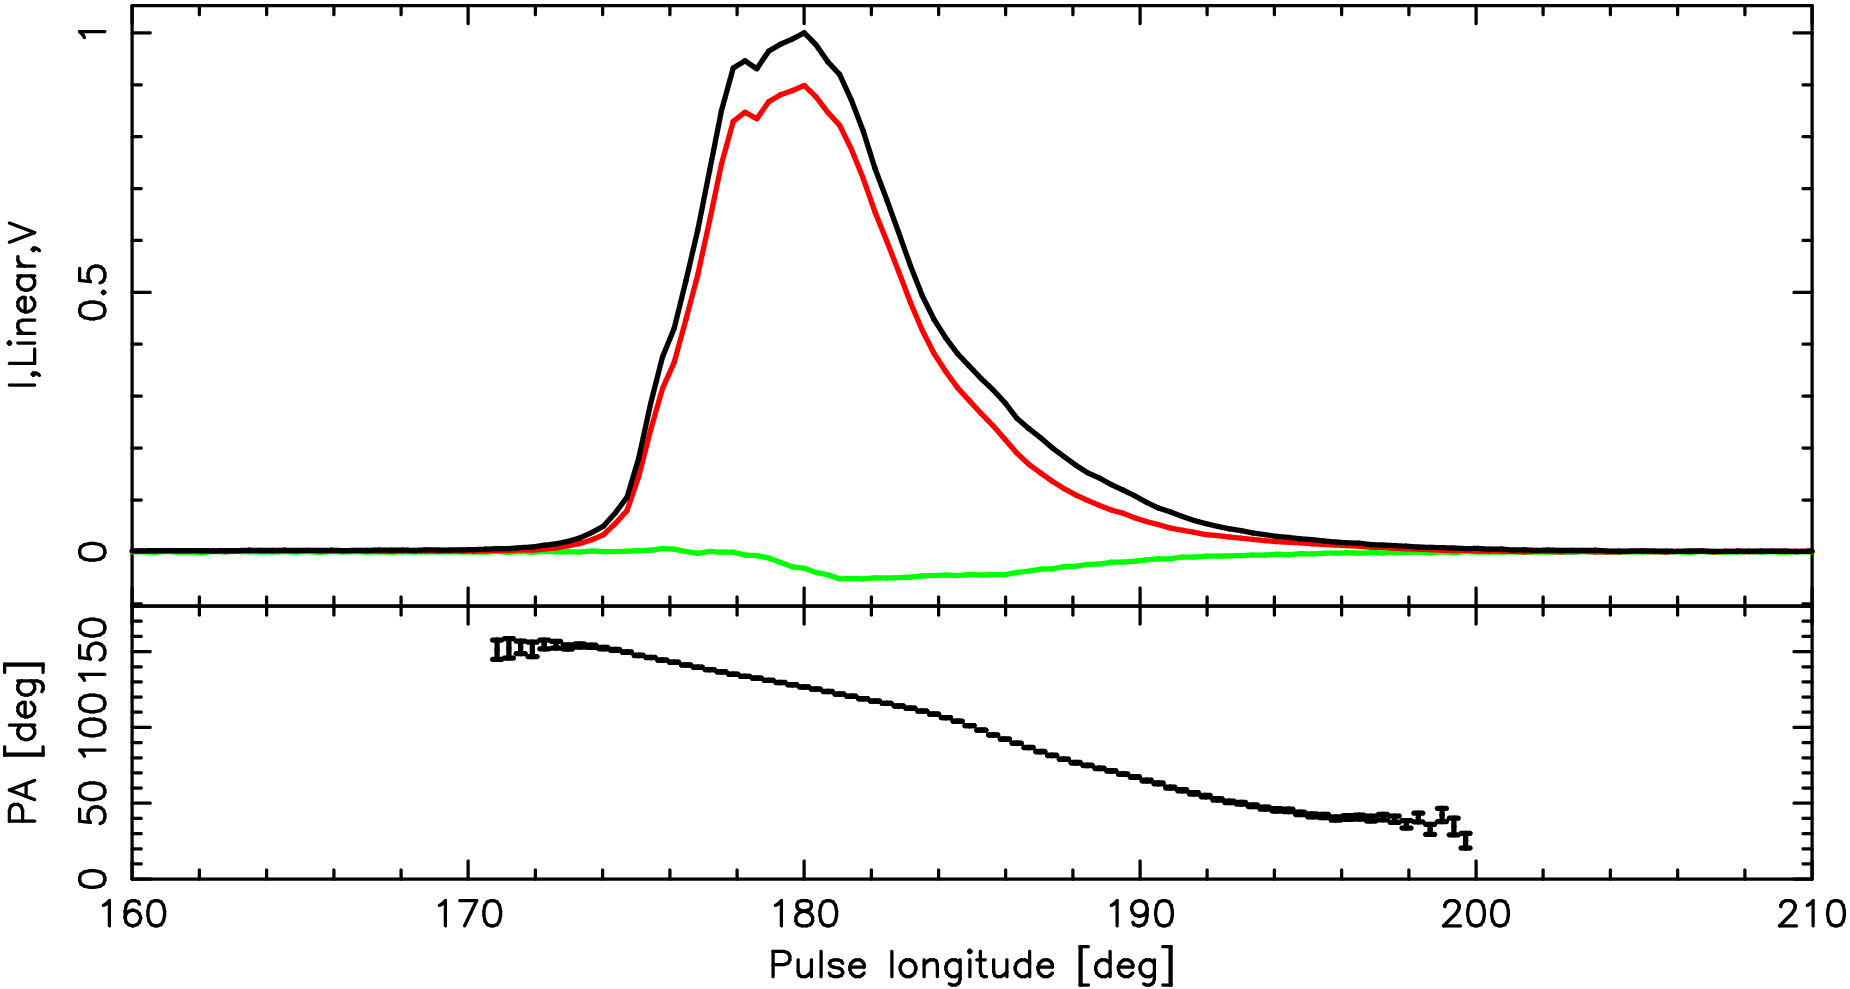
\includegraphics[width=0.8\textwidth]{Figures/Introduction/vela.png}
        \caption[The polarisation properties of the Vela pulsar]{The highly polarised profile of the Vela pulsar (PSR~B0833$-$45) at 1375~MHz. The upper panel shows the total intensity profile, linear polarisation, and circular polarisation by the black, red, and green lines respectively. The lower panel shows the PA of the linear polarisation, illustrating how it varies smoothly as a function of pulse longitude. This data was recorded by \citet{KJxx2006}, and is publicly available from the European Pulsar Network Database\footnotemark.}
        \label{fig: intro - vela polarisation}
    \end{center}
\end{figure}

\footnotetext{\url{http://www.epta.eu.org/epndb/}}\citet{RCxx1969} showed that the PA curve can be fitted well by a very simple, geometric model: the Rotating Vector Model (RVM). The RVM is built upon the following assumptions: first, each magnetic field line lies in a single plane containing the magnetic axis (as would be the case for a static, dipolar magnetic field). Second, this plane defines the orientation of linear polarisation of any radiation emitted from the vicinity of this field line \citep[e.g.][]{Cxxx2015}. From the point of view of an observer looking down on the star, the magnetic field lines surrounding the pole would appear radially projected. As the line of sight traverses this area, the angle of the observed field line changes smoothly, by up to $180\degr$. This is illustrated in Fig.~\ref{fig: intro - RVM field line schematic}.
\begin{figure}
    \begin{center}
        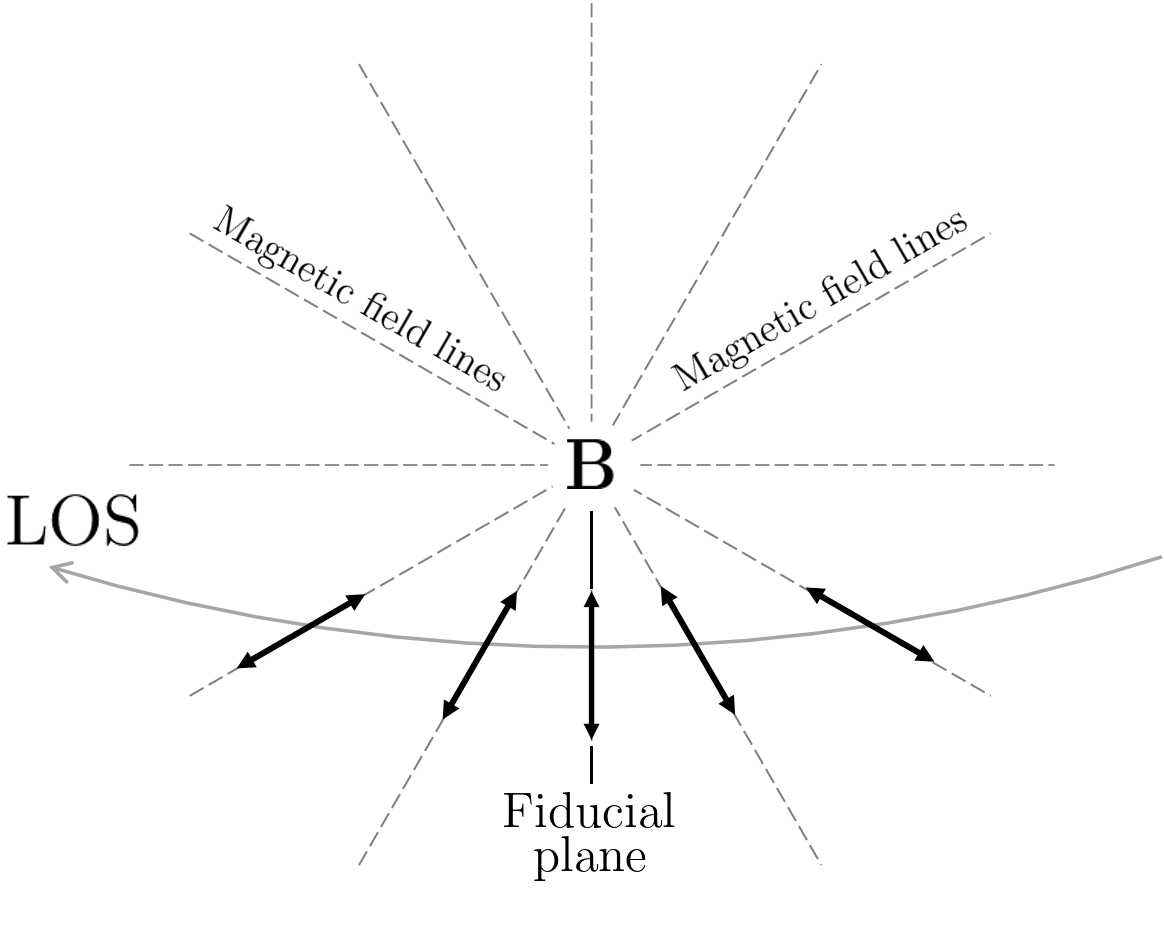
\includegraphics[width=0.75\textwidth]{Figures/Introduction/PA_curve_illustration}
        \caption[The Rotating Vector Model]{An illustration of the change in orientation of the magnetic field lines seen by the observer as the line of sight passes over them. The orientation of the field lines defines the direction of linear polarisation of the radio emission (thick black arrows), which changes smoothly as a function of pulse longitude.}
        \label{fig: intro - RVM field line schematic}
    \end{center}
\end{figure}
The shape of the PA curve and the RVM depends on the viewing geometry of the star, $\alpha$ and $\beta$. \citet{Kxxx1970} showed that the change of PA, $\psi$, as a function of pulse longitude, $\phi$, can be described by 
\begin{equation}
    \label{eq: intro - RVM}
        \tan(\psi - \psi_0) = \frac{\sin(\phi-\phi_0)\sin\alpha}{\sin(\alpha+\beta)\cos\alpha-\cos(\alpha+\beta)\sin\alpha\cos(\phi-\phi_0)},
\end{equation}
which describes a monotonic, S-shaped curve with an inflection point at ($\phi_0$, $\psi_0$). The maximum rate of change of the PA occurs when the observer's line of sight crosses the fiducial plane formed between the magnetic and rotation axes,
\begin{equation}
    \label{eq: intro - RVM gradient}
    \dphi{\psi}\bigg|_{\phi=\phi_0} = \frac{\sin\alpha}{\sin\beta}.
\end{equation}
Since the inclination angle $\alpha$ is constrained to lie between $0\degr$ and $180\degr$, $\sin\alpha$ is always positive, and therefore the sign of Eq.~\eqref{eq: intro - RVM gradient} depends only on the sign of $\beta$. In principle, fitting Eq.~\eqref{eq: intro - RVM} to the observed PA as a function of pulse longitude of a given pulsar can be used to determine the geometry, $\alpha$ and $\beta$ \citep[e.g.][]{EWxx2001, JWxx2006,RWJx2015a}. However, often the PA curve is only observed for a small fraction of a full rotation of the star (limited by the `duty cycle' of the pulses), and only its steepest gradient is well constrained. This necessitates further constraints to be applied using other methods. This is explored for the newly discovered pulsar PSR~J1926$-$0652 in Chapter~\ref{chapt: J1926}, and for the slow pulsar PSR~J0250+5854 in Chapter~\ref{chapt: J0250}.

Equation~\eqref{eq: intro - RVM gradient} suggests that the inflection point of the RVM curve should occur at the same pulse longitude as the fiducial plane of the total intensity pulse profile, $\phi_\mathrm{fid}$. However, observations show a small delay: $\Delta\phi = \phi_0 - \phi_\mathrm{fid}$. \citet{BCWx1991} modelled this delay as arising from relativistic aberration and retardation effects, and showed that it is dependent on the emission height $h_\mathrm{em}$
\begin{equation}
    \label{eq: intro - BCW shift}
    \Delta\phi = \frac{8\pi h_\mathrm{em}}{cP} = \frac{4h_\mathrm{em}}{R_\mathrm{LC}}.
\end{equation}

\subsubsection{Orthogonal polarisation modes}
\label{sec: intro - emission models - polarisation - OPMs}

Many pulsars -- especially those which are younger and more energetic -- have PA curves that can be closely modelled by the RVM. 
However, some pulsars are observed which show a rapid change in PA as a function of pulse longitude, of approximately $90\degr$. 
Early studies of Arecibo polarisation data by \citet{RCBx1974} and \citet{BRCx1976} suggested the existence of two nearly orthogonal emission modes which change in relative intensity across the profile.
These competing polarisation modes distort the `fundamental' RVM curve, causing a rapid transition between states: when the dominant mode changes, a jump in the average PA occurs. This can be seen for example in the integrated profile of PSR~J0742$-$2822 as shown in Figure \ref{fig: intro - J0742 OPMs}.
\begin{figure}
    \begin{center}
        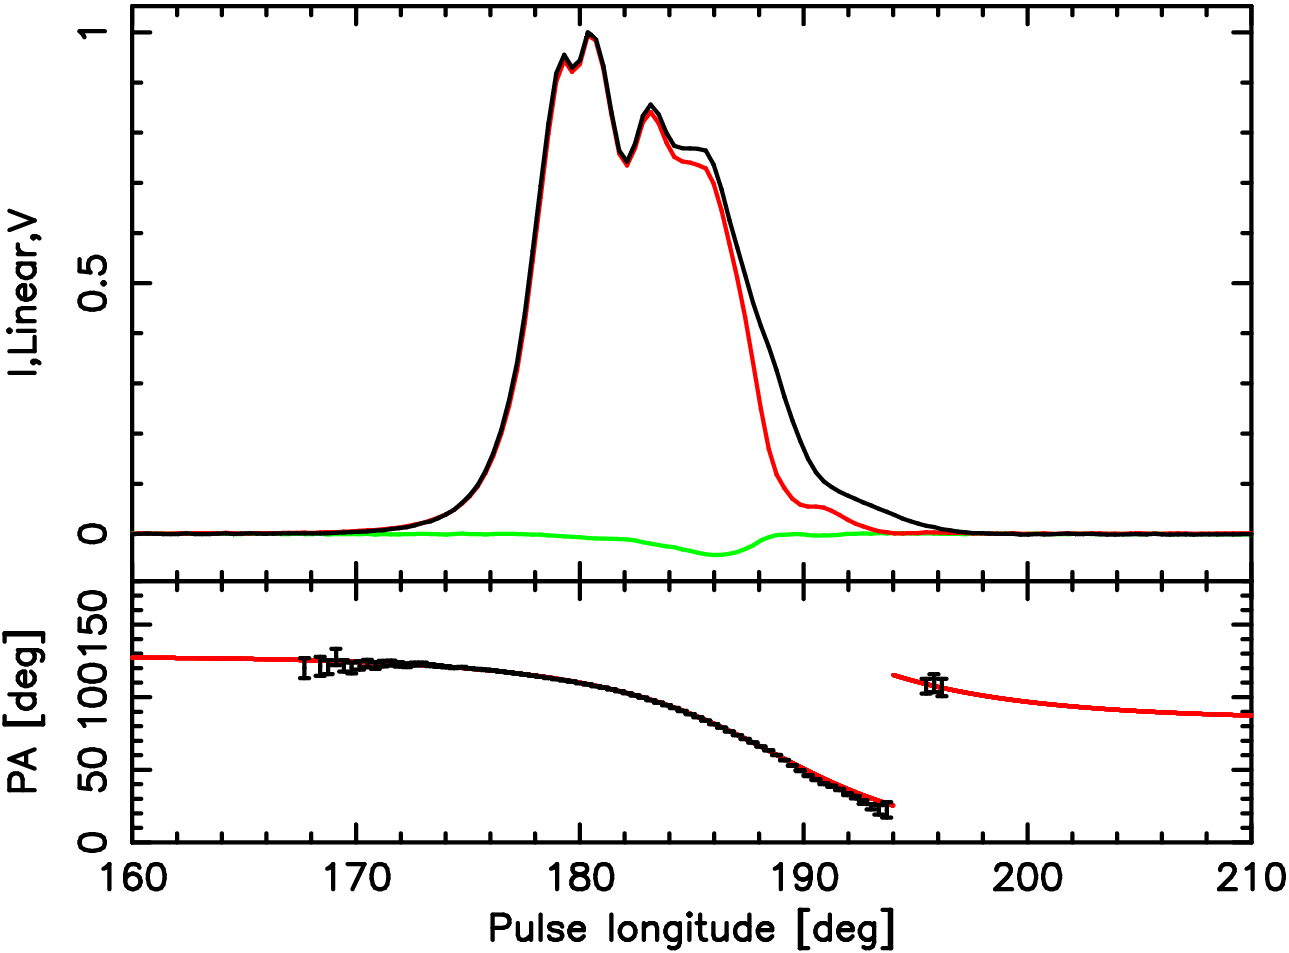
\includegraphics[width=0.6\textwidth]{Figures/Introduction/opm_profile}
        \caption[Orthogonal polarisation modes in PSR~J0742$-$2822]{The profile of PSR~J0742$-$2822 at a wavelength of 20~cm as observed by \citet{RWJx2015a}. In the upper panel total intensity is shown in black, linearly polarised intensity in red, circular polarisation in green. The lower panel shows the position angle as a function of pulse longitude, and the red line is the best-fitting RVM curve. An orthogonal mode transition can be seen at around pulse longitude $195\degr$. }
        \label{fig: intro - J0742 OPMs}
    \end{center}
\end{figure}

\citet{MSxx2000} showed that the two modes can exist simultaneously, but in general the intensity ratio between them depends on pulse longitude. When the two modes are viewed simultaneously, the subsequent incoherent mixing of the orthogonal polarisations means that the resulting observed signal becomes depolarised. This reinforces the suggestion that the emission is intrinsically highly polarised \citep[e.g.][]{BRxx1980,SCR+1984, MSxx1998}.
A possible explanation for the origin of OPMs was given by \citet{Mxxx1979} and \citet{ABxx1986}, who proposed that the distinct modes are caused by the difference in ray paths of natural modes in plasma. Waves in an ultra-relativistic plasma propagate via two modes; the `ordinary' (O-) mode, and the `extraordinary' (X-) mode, which are orthogonal. In the presence of a strong magnetic field, such as is found in pulsar magnetospheres, the X-mode decouples from the plasma and propagates freely. However, the O-mode remains connected to the plasma and is therefore subject to refraction. The result is that the O-mode radiation follows a curved path whilst the X-mode follows a shorter, straight path from the point of emission. Although they may originate from the same location, the path length difference and curvature of the path means that an observer will see the two modes with different delays, giving the impression of two orthogonally polarised images of the same emission structure. This can lead to OPM jumps and asymmetry of the (polarised) pulse profile, as explored in Chapter~\ref{chapt: B0031}.


\subsubsection{Polarisation conventions in pulsar astronomy}
\label{sec: intro - emission models - polarisation - conventions}

Throughout this work, it has been very important to define reference frames and conventions for the various coordinate systems encountered. A large part of this thesis deals with polarisation data, and it is therefore prudent to discuss the coordinate systems and conventions used in pulsar astronomy. In 1969, the Institute of Electrical and Electronics Engineers (IEEE) defined a right-handed coordinate system for the propagation of radio waves \citep[][still valid as of 2019]{IEEE1969}. In this system the $x$-axis points towards the North and the $y$-axis points East (as projected onto the plane of the sky for an earthbound observer), whilst the $z$-axis extends towards the observer. The position angle of linear polarisation (PA; $\psi$) increases from the North towards the East, so \textit{anticlockwise} from the observer's perspective. This coordinate system is shown in Fig.~\ref{fig: intro - IEEE polarisation frame}.
\begin{figure}
    \begin{center}
        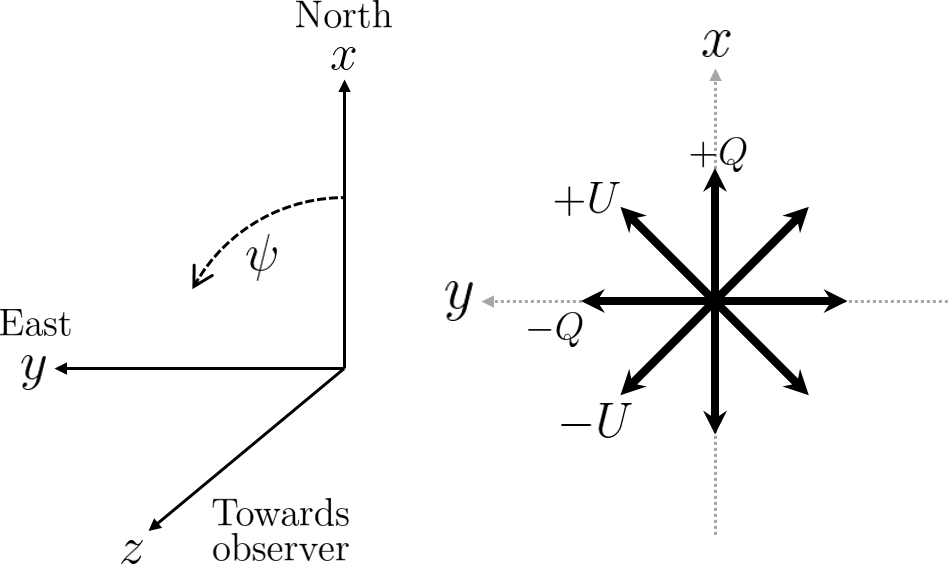
\includegraphics[width=0.6\textwidth]{Figures/Introduction/IEEE_coordinate_system}
        \caption[Reference frame of IEEE polarisation conventions]{The IEEE coordinate system which defines the position angle of linear polarisation ($\psi$) on the sky from the perspective of an earthbound observer (left). The right-hand panel shows the coordinate system that defines the linear Stokes parameters $Q$ and $U$. $+Q$ lies along the $x$-axis, while $-Q$ lies on the $y$-axis. $+U$ is oriented at $45\degr$ between the two. }
        \label{fig: intro - IEEE polarisation frame}
    \end{center}
\end{figure}
For right-handed circular polarisation, the PA of the electric field vector increases with time, forming a left-handed helix -- this implies that the $x$-component of the field leads the $y$-component. In this coordinate system, the linear Stokes parameters $Q,U$ are uniquely defined: positive $Q$ lies along the $x$-axis whilst negative $Q$ lies along the $y$-axis. Positive $U$ lies along the line $y=x$, where $\psi=\pi / 4$ \citep{HBxx1996}. The International Astronomical Union (IAU) adopted this definition \citep{IAU1974}, supplementing it with a definition of the sign of Stokes $V$: positive for right-handed circular polarisation \citep{Wxxx1973,TMSx1986}.

However, the early pulsar observations \citep[e.g.][]{Mxxx1971} established a convention in which Stokes $V$ is positive for left-handed circular polarisation as defined by the IEEE; opposite to that of the IAU convention. This alternate definition is the convention described by \citet{Kxxx1966} and is that used by the \textsc{psrchive} software package and encoded in the \textsc{psrfits} file format \citep{SMJR2010}. The consequences of a discrepancy between the geometry of the RVM and the IEEE polarisation convention were explored by \citet{EWxx2001}. They note that $\alpha$ and $\beta$ are both defined as increasing away from the positive spin axis of the pulsar, which points in the direction of the angular momentum vector (i.e. the North pole). This means that in the framework of the RVM as given by Eq.~\eqref{eq: intro - RVM} \citep{Kxxx1970}, the position angle $\psi$ is defined as increasing in the \textit{clockwise} direction (this was also pointed out by \citealt{DTxx1992} and \citealt{APTW1996}). The required correction to previously published geometries is $\alpha = 180\degr - \alpha_\mathrm{RVM}$ and $\beta = -\beta_\mathrm{RVM}$, where the subscript denotes values measured by fitting the RVM \citep{EWxx2001}. 
% This correction is highlighted where relevant in this thesis. \todo{MAKE SURE IT IS! C12 AND 0250}


\subsection{Single pulse phenomena}
\label{sec: intro - emission models - single pulse phenomena}

% Observation of drifting subpulses
The integrated pulse profile is characteristic and unique to each pulsar, and is typically stable and reproducible over many hundreds of pulse periods. However, it often hides a number of interesting features which vary on timescales comparable to $P$. The individual pulses of most radio pulsars are made up of several components, which are typically between $1\degr-3\degr$ in width, much narrower than the full profile width which spans the \textit{pulse window} typically covering around $10\degr$ in pulse longitude \citep[e.g.][]{KWJ+1994}. These components, known as `subpulses', can behave in different ways: they may appear at random locations within the pulse window; they may favour certain longitudes, consistently appearing in the same place in different pulses; or they may steadily drift across the pulse window at a roughly constant rate. This last case is the phenomenon of \textit{drifting subpulses}, which are believed to occur in more than 55~per~cent of pulsars \citep{WESx2007}, and is a feature of great interest in this thesis.

Drifting subpulses were first noted by \citet{DCxx1968} in pulsars CP~1919+21 and AP~2015+28, and define two more important periodicities. The separation between subpulses within a given pulse is labelled $P_2$, whilst the number of pulses it takes for a particular pattern of subpulses to repeat is labelled $P_3$ \citep{SSPW1970} -- these quantities are illustrated in Fig.~\ref{fig: intro - drifting subpulses}. In this nomenclature, the pulsar rotation period $P$ is also called $P_1$ \citep{Bxxx1973}, a convention used in this thesis hereafter. Figure~\ref{fig: intro - drifting subpulses} shows a `pulse stack', created by splitting the time series data into blocks of length equal to one stellar rotation period, so each block contains a single pulse. The individual pulses are typically stacked as shown, with the pulse number (i.e. time) increasing vertically upwards. This allows systematic deviations in pulse profile shape to be identified easily -- if drifting subpulses are present, they will form diagonal bands in the pulse stack, referred to as `driftbands'.  
\begin{figure}
	\centering
	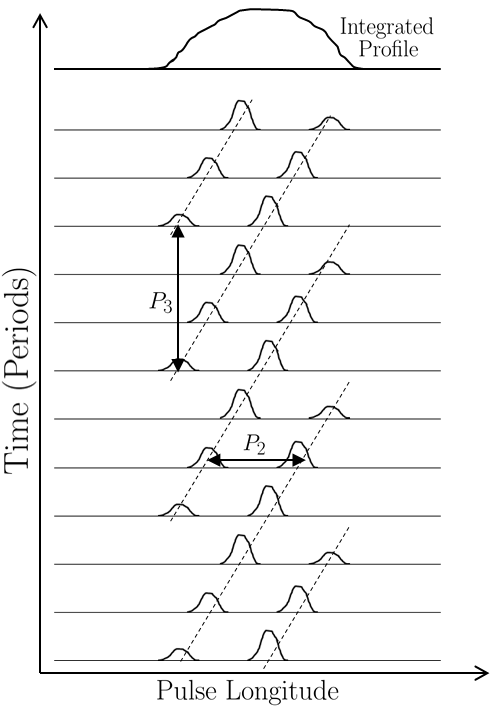
\includegraphics[width=0.4\textwidth]{Figures/Introduction/drifting_subpulses}
    \caption[Drifting subpulses and the definitions of $P_2$ and $P_3$]{An illustration of drifting subpulses showing the periods $P_2$ and $P_3$, where $P_2$ is the spacing between successive subpulses and $P_3$ is the spacing between driftbands (indicated by dotted lines). As is conventional in pulsar astronomy, time increases upwards in the plot. The top of the plot shows the integrated profile \citep[after][]{Bxxx1973}.}
    \label{fig: intro - drifting subpulses} 
\end{figure}

Some pulsars exhibit an abrupt cessation of emission within a single period. Known as `nulling', this was first reported by \citet{Bxxx1970b} and is now believed to be a relatively common feature, seen in approximately 8~per~cent of the population \citep[e.g.][]{Rxxx1976, Bxxx1992, LWxx1995, WMJx2007, GJKx2012, SMxx2021}. The length of null has been seen to vary significantly across the population, from several periods to days, months, or even years. The portion of time that a pulsar is nulling is referred to as its `nulling fraction' and varies from near zero (PSR~B1737+13, \citealt{Bxxx1992}) to over 90~per~cent (PSR~B1713$-$40, \citealt{WMJx2007}). Nulling is believed to be an extreme form of profile `mode switching', where the pulsar has two or more distinct stable profile shapes. This was first observed in PSR B1237+25 by \citet{Bxxx1970b} and largely affects the normal, longer-period pulsars, although it has also been reported in some MSPs \citep[e.g][]{KLL+1999,MKMP2018, BMRx2019}. If the pulsar shows drifting subpulses, a mode-switch may be associated with a change in the drifting behaviour. PSR~B0031$-$07 is one such pulsar that is explored in detail in Chapter~\ref{chapt: B0031}. This pulsar has three distinct drift modes with $P_3 \approx 12 P_1$, $P_3 \approx 7 P_1$, and $P_3 \approx 4 P_1$ \citep{HTTx1970, VKxx1997,SMKx2005, SMS+2007, MBT+2017,MBW+2019}.





\subsubsection{The carousel model}
\label{sec: intro - emission models - single pulse phenomena - carousel model}

% The drifting subpulse phenomenon can be attributed to the breakdown of the strong electric field in the polar gap through localised `sparks'. These sparks are the sites of pair production, creating the bunches of particles that are accelerated by the fields and give rise to coherent radio emission in sub-beams in the open-field-line region \citep{RSxx1975, CRxx1977, Bxxx1982, FRxx1982,GSxx2000}. Under the action of $\mathbf{E} \times \mathbf{B}$ drift, these sparks complete one full circulation around the magnetic axis in a period $P_4$. 
The drifting subpulse phenomenon can be attributed to the breakdown of the strong electric field in the polar gap through localised `sparks'. These sparks are the sites of pair production, creating the bunches of particles that are accelerated by the fields and give rise to coherent radio emission in sub-beams in the open-field-line region \citep{RSxx1975, CRxx1977, Bxxx1982, FRxx1982,GSxx2000}.

These sparks circulate round the magnetic axis under the action of $\mathbf{E} \times \mathbf{B}$ drift, caused by the large potential difference $\Delta V \approx 10^{12}$~V across the gap \citep{RSxx1975}, and can be explained as follows. To a stationary observer the magnetic field is assumed to be time-independent (as it would be if it were axisymmetric about the rotation axis), and this is taken to be true for small inclination angles \citep{RSxx1975}. In that case, a closed integral of the resulting electric field $\oint \mathbf{E}\cdot d \mathbf{l} = 0$. Similarly, the change in the electric field due to the potential across the polar gap must also satisfy
\begin{equation}
    \label{eq: intro - zero E field circulation}
    \oint \Delta\mathbf{E}\cdot d \mathbf{l} = 0.
\end{equation}
Consider a closed integral of the electric field, following a path which touches the edge of the polar cap and the pulsar's surface, as shown in Fig.~\ref{fig: intro - polar gap integral}. This assumes a small polar cap and low altitudes, such that the magnetic field lines may be assumed to be perpendicular to the stellar surface across the diagram.
\begin{figure}
	\centering
	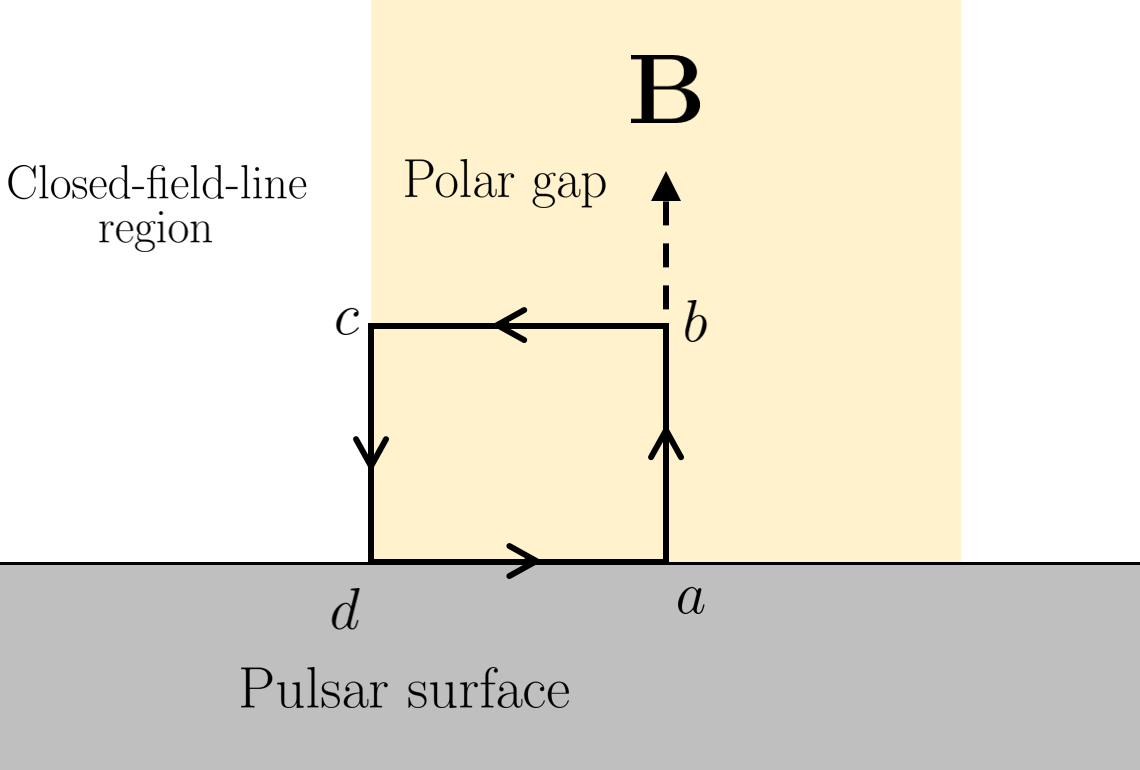
\includegraphics[width=0.5\textwidth]{Figures/Introduction/polar_gap_integral}
    \caption[Closed integral of the electric field in the polar gap]{A schematic view of a closed integral of the electric field in the polar gap, between the points $a$, $b$, $c$, and $d$. The potential drop $\Delta V$ due to the polar gap is directed along $ab$, and the distance $bc$ is the radius of the polar cap, $r_p$. The magnetic field lines are assumed to be perpendicular to the stellar surface, and remain parallel across the diagram.}
    \label{fig: intro - polar gap integral} 
\end{figure}

Since the star is a perfect conductor, $\Delta \mathbf{E} = 0$ along the segment $da$.  Outside (and at the boundary of) the polar cap, the assumption is that the closed-field-line region is co-rotating with the star \citep{GJxx1969}. This means that $\mathbf{E}\cdot\mathbf{B} = 0$, hence $\Delta \mathbf{E} = 0$ along the segment $cd$ also. Therefore, in order to satisfy Eq.~\eqref{eq: intro - zero E field circulation},
\begin{equation}
    \label{eq: intro - balanced E fields}
    \int^b_a \Delta\mathbf{E}\cdot d \mathbf{l} = -\int^c_b \Delta\mathbf{E}\cdot d \mathbf{l}.
\end{equation}
The left-hand side of the equation is simply the potential drop in the centre of the gap, $\Delta V$. The right hand side is the drop in the electric field in the horizontal direction, $\Delta E_x$, integrated between the centre and edge of the polar cap with radius $r_p$. Under the assumption that this field is roughly constant, this has the approximate result $r_p \Delta E_x$. This means that there is an electric field component directed parallel to the stellar surface across the polar cap, with magnitude $\Delta E_x = \Delta V / r_p$. The vertical component of $\Delta E$ in the polar gap, $\Delta E_y$, is responsible for accelerating the charged particles along the magnetic field lines. The drift velocity \citep[e.g.][]{Cxxx2016} of a charged particle (and hence the sparks) in the polar cap due to the combination of this electric field and the pulsar's magnetic field is
\begin{equation}
    \label{eq: intro - E cross B drift}
    \mathbf{v} = \frac{\mathbf{E} \times \mathbf{B}}{B^2}c.
\end{equation}
Overall, the average drift velocity of the sparks around the polar cap is
\begin{equation}
    \label{eq: intro - spark speed}
    \Delta v \approx \frac{\Delta V} {B_\mathrm{S} r_p}c,
\end{equation}
and they complete one full circulation around the magnetic axis in a period
\begin{equation}
    \label{eq: intro - P4 from RS model}
    P_4 = \frac{2\pi B_\mathrm{S} r_p^2}{c\Delta V} \approx 5.6\times10^{-12}\frac{B_\mathrm{S}}{P_1}\text{\ seconds},
\end{equation}
where we have assumed the magnetic field strength is that at the stellar surface (Eq.~\eqref{eq: intro - characteristic B field}) \citep{RSxx1975}. This simple picture has been developed over the years \citep[e.g.][]{GSxx2000, Kxxx2009, Sxxx2013}, but the central picture remains the same: the sparks are distributed around the polar cap, forming a `carousel' of sub-beams that circulates as the pulsar rotates.

If the circulation time is slow, then $P_4 = NP_3$, where $N$ is the number of sub-beams and $P_3$ is the time it takes for a given spark to move round to the same position as its predecessor. The carousel is believed to circulate in the same direction as, but slightly slower than, the pulsar spins. If the number of sub-beams is high, or the circulation speed is rapid, this can lead to aliasing. Aliasing in the context of the rotating carousel describes a stroboscopic effect whereby a quickly circulating carousel, sampled once each stellar rotation ($P_1$) would appear to be moving much slower than it actually is, potentially even appearing to move in the opposite direction. More details on the effects of aliasing are given in Appendix~\ref{app: geometry derivations}. The classical picture of the carousel beam structure is shown in Fig.~\ref{fig: intro - carousel schematic} and consists of multiple evenly spaced sub-beams arranged on the polar cap in one or more nested cones. Figure~\ref{fig: intro - driftband schematic} shows how this structure leads to driftbands in the pulse stack.
\begin{figure}
	\centering
	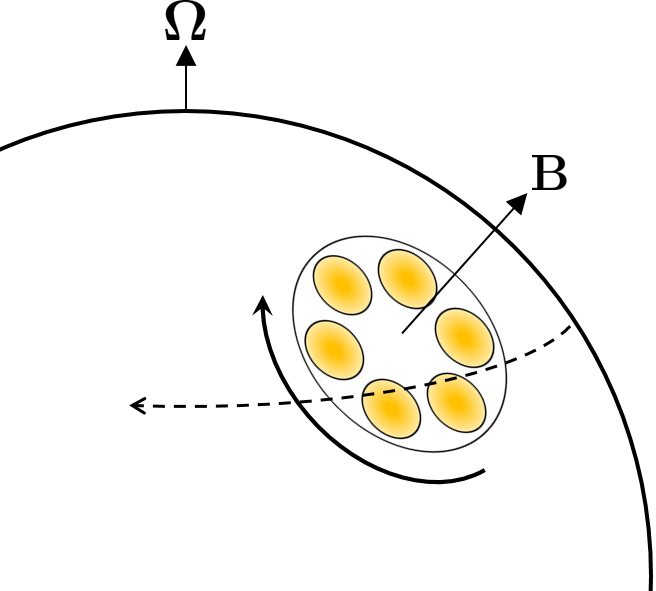
\includegraphics[width=0.5\textwidth]{Figures/Introduction/carousel_schematic}
    \caption[A carousel of sub-beams]{An illustration of a carousel of sparks circulating around the magnetic pole in the polar cap. As the carousel circulates, the observer's line of sight (dashed line) passes over different sub-beams at different times.}
    \label{fig: intro - carousel schematic} 
\end{figure}
As well as drifting subpulses \citep[e.g.][]{GSxx2000,GMxx2001,WESx2006,WSEx2007}, the carousel model is able to explain many other observed phenomena. `Bidrifting' pulsars, which show simultaneous drifting in opposite directions, can be explained by elliptical carousels \citep{QLZ+2004, Wxxx2016, WWxx2017, SLxx2017, SLWM2020} and periodic nulling can be explained by the extinguishing of one or more sub-beams as the carousel circulates, giving rise to nulls that last an integer multiple of $P_3$ cycles \citep{HRxx2007, HRxx2009, RWxx2008}.

In order to gain a clearer understanding of the physics of the carousel, it is useful to recreate an image of it. By considering the path the footprint of the observer's line of sight takes through the emission region, \citet{DRxx1999} defined a cartographic transform to map the observed intensity at a certain pulse longitude in a given pulse to a position on the polar cap. In Appendix~\ref{app: geometry derivations} I show how this transform is derived from first principles, and extend it to the case of short circulation times where aliasing is occurring, and also demonstrate how it may be applied to data folded at the period $P_3$ (see Sec.~\ref{sec: intro - emission models - single pulse phenomena - P3 folding}). 

\citet{DRxx2001} used this transform to study the structure of PSR~B0943+10 in two different drift modes -- the `bright' (B) mode and the `quiescent' (Q) mode -- at 430~MHz. This pulsar has an average $P_3 = 11.1 P_1$, although the authors argue aliasing is taking place. They made an image of the B mode carousel with 20 sparks, and a circulation time $P_4 = 37 P_1$, and the Q mode was also compatible with this structure. Their multi-frequency analysis revealed a similarity of the sub-beams at different frequencies and suggested that the radiation is produced from columns of plasma, which in turn implies the existence of some form of `seeding' mechanism at the stellar surface. The authors argue that the sub-beam emission is therefore bound neither to the magnetic field, nor the stellar surface.

\subsubsection{Subpulse polarisation}
\label{sec: intro - emission models - single pulse phenomena - subpulse polarisation}

Compared to the integrated pulse profile, individual pulses exhibit a higher degree of polarisation \citep[see][]{PulsarAstronomy}. This is to be expected since the polarisation vector $\mathbf{p}$ varies somewhat between pulses, and vector addition of many will therefore lead to depolarisation. \citet{THHM1971} examined the subpulses of PSR~B0809+74 and found that the successive drifting bands display almost identical polarisation behaviour, having a high degree of linear polarisation and showing a systematic PA swing with a negative gradient through each subpulse. The PA at the leading edge of each subpulse was approximately the same, as was its rate of change, such that all subpulses showed roughly the same position angle near their peaks. A small amount of circular polarisation was visible near the centre of each pulse window. \citet{RRS+2002} argued that the linear polarisation angles of the drifting subpulses are oriented according to the stellar magnetic field. Furthermore, they showed that the subpulses of PSR~B0809+74 contain two orthogonal modes of polarisation (OPMs) which arise from emission directed either parallel or perpendicular to the magnetic field lines. They find that the OPM transitions occur at progressively earlier phases in successive pulses, remaining almost parallel to the driftbands and therefore at the same position within subpulses as they drift across the pulse window. This was what was observed by \citet{THHM1971}, albeit somewhat smeared. The two modes gradually mix across the profile window as subpulses at the edges tend to show only one of the modes. The sign of the circular polarisation is closely correlated with the power of the two linear modes, while being slightly displaced in pulse longitude.

\citet{RRL+2006} expanded the analysis of PSR~B0809+74, attempting to map the emission region surrounding the magnetic pole, using the cartographic transforms of \citet[][see Appendix~\ref{app: geometry derivations}]{DRxx2001}. They found two possible configurations of the carousel: 8 to 10 sub-beams for an `outer' (equatorward) traverse of the line of sight (LOS), and 25 to 40 sub-beams for an `inner' (poleward) traverse. They found that one OPM is strongly associated with the overall intensity pattern, forming roughly azimuthally symmetric patches on the inner edge of the observed emission (limited by the fact that the minimum approach of the LOS to the magnetic axis is $\beta$ and therefore some emission is never seen). In contrast, the other OPM is radially extended and is strongest between the total power beamlets. The authors did not attempt to provide a physical explanation for the observed structure, but did note that the azimuthal and radial offset between modes is as expected from an earlier independent analysis of polarised conal profiles \citep{RRxx2003}. This OPM behaviour could potentially be explained by the O- and X-mode propagation introduced in Sec.~\ref{sec: intro - emission models - polarisation - OPMs}, in which the two modes would appear as offset images of the same carousel.



\subsubsection{\texorpdfstring{$P_3$-folding}{P3-folding}}
\label{sec: intro - emission models - single pulse phenomena - P3 folding}

In order to more clearly see the shape of driftbands the technique of `$P_3$ folding' can be used. In this method the data are averaged over many modulation cycles to produce an image of the average driftband, with a higher signal-to-noise ratio (S/N) than for the individual driftbands. This technique, while seemingly simple in principle, can be complicated by the fact that the $P_3$ periodicity is rarely stable, often fluctuating somewhat about a mean value over the course of an observation. If such data were naively folded with a fixed period, the variations can cause smearing of the driftband (see \citealt{DRxx2001} and \citealt{LKR+2002} for example). However, a method to do $P_3$ folding whilst taking into account these variations was first used by \citet{HSW+2013} to study PSR~B0809+74, which exhibits a somewhat variable $P_3$. This method is implemented in the \textsc{psrsalsa}\footnote{\url{https://github.com/weltevrede/psrsalsa}} suite of programs \citep{Wxxx2016} used throughout the work in this thesis, and works in the following way.

First, the rough $P_3$ value of interest is identified, typically using Fourier techniques such as the longitude-resolved fluctuation spectrum (LRFS; see Chapter~\ref{chapt: J1926}). The pulse stack is then divided into blocks of some integer multiple of $P_3$; $n\times P_3$. For example, if $P_3 = 12.6 P_1$, one might choose a block length of 38 pulses which encloses $ 3\times P_3$. When dividing the pulse stack care should be taken to ensure the blocks form continuous pulse sequences (i.e. nulls and mode changes are removed). Each block is then folded with a fixed period $P_3$. This initial crude folding increases the S/N of the driftbands within the block, which is beneficial when performing the cross-correlations as described below. On the other hand, if the $P_3$ variation timescales are short, then this fixed-period folding can lead to smearing, so some care must be taken in the choice of $n$. In practice, different block lengths are tried to visually judge the optimum compromise. Variations in $P_3$ are taken into account by cross-correlating the folded blocks and allowing an offset in pulse number before stacking them. This is an iterative process: the output from the first iteration is taken as a template for the next iteration, where the blocks are correlated with the template in order to determine their offsets. The benefit of this method is that the template will have a higher S/N ratio than the individual blocks, so alignment is more reliable after the initial pass. The rate of improvement decreases with subsequent iterations, so the number of iterations is chosen such that further processing would not significantly improve the results.

An illustration of how a carousel leads to drifting subpulses and hence driftbands in the pulse stack is shown in Fig.~\ref{fig: intro - driftband schematic}. The figure also indicates how the stack is broken up into blocks and formed into a $P_3$-fold.

\begin{figure}
	\centering
	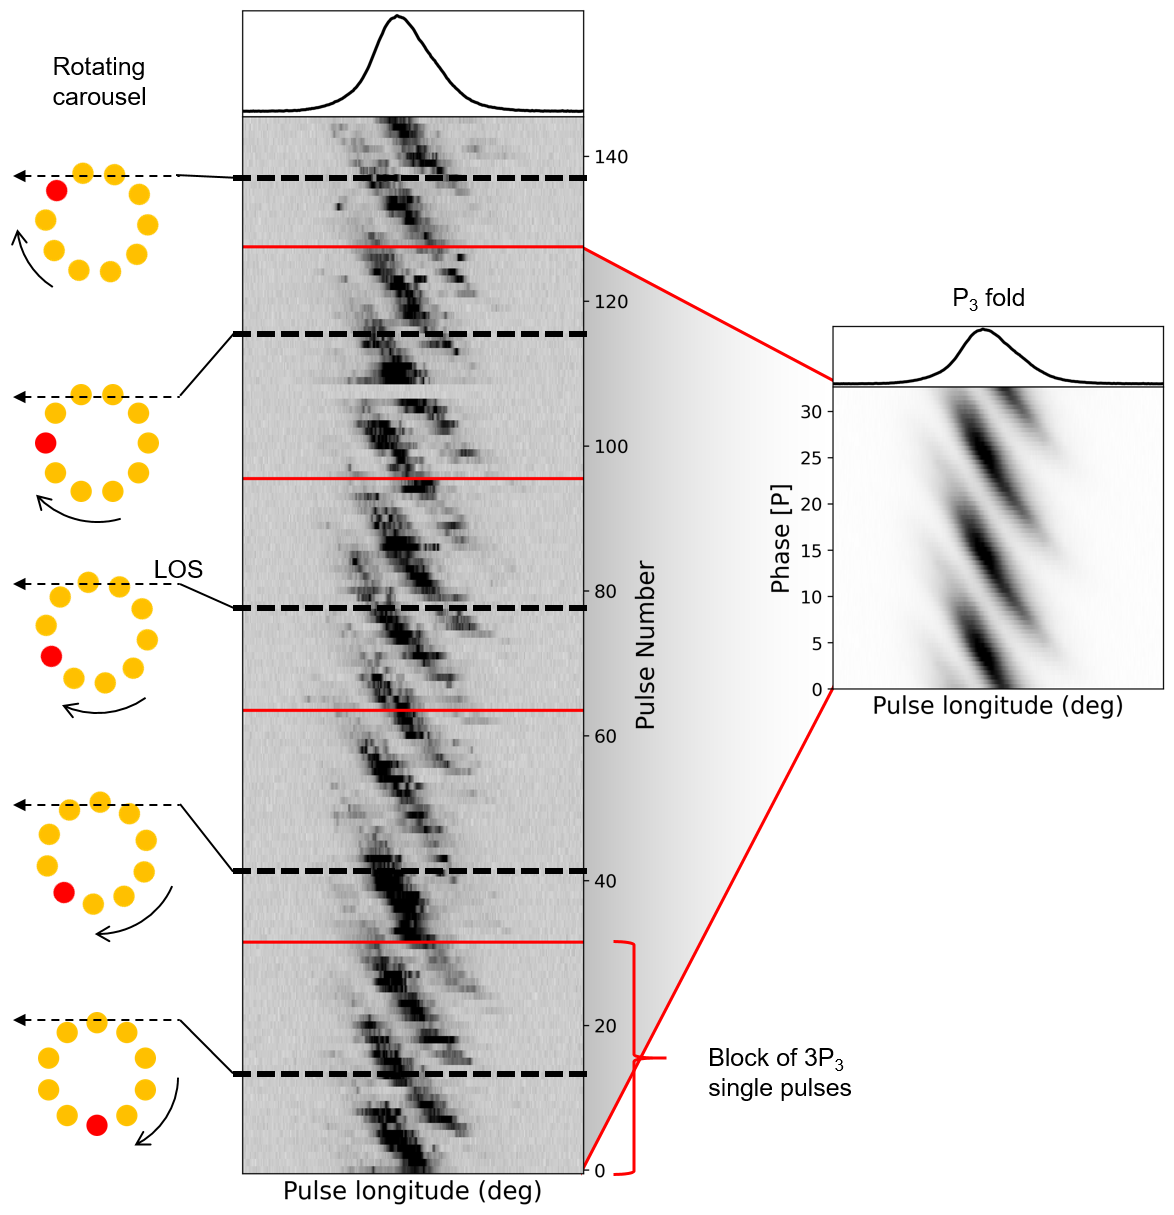
\includegraphics[width=1.0\textwidth]{Figures/Introduction/car2p3fold}
    \caption[Driftbands produced by a carousel and $P_3$-folding of a pulse stack]{An illustration of how a carousel-like structure leads to driftbands in the pulse stack, and how this is then folded at the period $P_3$ in order to show the average driftband with a higher S/N. As the carousel (left) slowly rotates (one sub-beam is coloured red to help illustrate this), the LOS (dashed black lines) intercepts different sub-beams at different times. The movement of the sub-beams along the LOS gives rise to the driftbands in the pulse stack (centre), separated by $P_3/P_1$ pulses as explained in Sec.~\ref{sec: intro - emission models - single pulse phenomena - carousel model}. In this example, blocks of length $3P_3$ were folded, aligned using cross-correlations, and summed to create a $P_3$-fold (right) as detailed in Sec.~\ref{sec: intro - emission models - single pulse phenomena - P3 folding} -- here three $P_3$ cycles are shown for clarity. The data shown here is an observation of PSR~B0809+74 at 328~MHz, performed with the Westerbork Synthesis Radio Telescope in November 2000 \citep{RRS+2002}.}
    \label{fig: intro - driftband schematic} 
\end{figure}

\section{Observation processing}
\label{sec: intro - observation processing}

To properly study the properties of radio pulsars, the observations must first be calibrated, and corrections made for a number of propagation effects. Both flux density calibration and polarisation calibration are commonly performed on the raw recorded data, and frequency-dependent effects such as dispersion and Faraday rotation must be removed in order to study the \textit{intrinsic} properties of the emission.

\subsection{Polarisation calibration}
\label{sec: intro - observation processing - polarisation calibration}

Pulsar polarisation can provide a wealth of information on the underlying emission physics and the propagation through the interstellar medium (ISM), but first it must be properly calibrated. In general, the measured Stokes parameters will differ from the intrinsic Stokes parameters of the source for a variety of reasons, primarily related to the properties of the receiver and the observing system. A common type of receiver is a linear feed, which consists of a pair of crossed dipole antennas used to detect the orthogonal electric field components of the incoming signal, $E_x$ and $E_y$. From these quantities the four Stokes parameters can be calculated using Eqs.~\eqref{eq: intro - stokes I linear}--\eqref{eq: intro - stokes V linear}.

The Stokes parameters can be presented as a vector. The intrinsic Stokes vector is transformed to the observed (un-calibrated) Stokes vector by the Mueller matrix \citep{Mxxx1948}, a $4\times4$ real-valued matrix of which seven elements are independent and describe the effect of the signal chain on $E_x$ and $E_y$. Calibrating the observing system determines the frequency-dependent Mueller matrix, allowing the intrinsic Stokes vector to be calculated. The first of the seven independent values is the overall gain of the system, and its calibration is known as flux calibration (see Sec.~\ref{sec: intro - observation processing - flux calibration}).

Four parameters are known as `leakage' parameters. These describe the situation where the signal attributed to one of the dipoles appears in the output from the other dipole, due to cross-coupling of the supposedly orthogonal elements. An example would be where, for an incident wave which is totally linearly polarised in the vertical direction, the horizontal dipole registers a signal. The leakage parameters are specific to a given receiver and signal chain, so are a relatively constant property of the system and do not need to be measured for individual observations. It is impossible to eliminate all leakage, although careful instrument design can minimise its effects \citep[e.g.][]{RTxx2018}. 

The remaining two parameters in the Mueller matrix are the differential gain and differential phase. The differential gain describes slight differences in the sensitivity and amplification of the two orthogonal polarisation signals, whilst the differential phase accounts for lag between the two channels (as a result of different cable lengths for example). These effects can be measured by performing a calibration observation just before, or after, the actual observation of the pulsar. The calibration observation should be a pointing to a position at least one beam width away from the source of interest, but close enough that the properties of the background radio emission are similar. During this pointing the signal from a `noise diode' is recorded -- this is a pulsed signal with a known strength and polarisation that is artificially injected into the signal chain. If it is injected equally into the two dipoles (i.e. at an effective orientation of $45\degr$), then it is known that the output signal should be pure Stokes $U$ (see Eqs.~\eqref{eq: intro - stokes I linear}--\eqref{eq: intro - stokes V linear}). Deviations from this pure signal allow the differential gain and phase to be calculated. 

Combined, the leakage parameters and the differential gain and phase form the `receiver solution' which can be applied to raw data in order to calibrate its polarisation properties. One final effect that, depending on the telescope, must be accounted for is the rotation of the feed with respect to the sky in long tracking observations. This effect, known as `parallactic angle' rotation, affects any `alt-azimuth' telescope unless the feed is rotated during the observation. This correction is to compensate for the changing orientation of the feed with respect to the sky. For example, the 19-beam receiver on the Five-hundred-metre Aperture Spherical radio Telescope (FAST) is designed to rotate to keep the orientation of the feed relative to the source fixed over the course of a tracking observation \citep[e.g.][]{JYG+2019}.


\subsection{Flux calibration}
\label{sec: intro - observation processing - flux calibration}

Knowing the absolute flux density of a pulsar is necessary for calculating its spectral index, and examining its frequency evolution (see for example the work on PSR~J0250+5854 in Chapter~\ref{chapt: J0250}).
The simplest way of calculating the flux density of a pulsar is to use the radiometer equation \citep{Dxxx1946}. This can be adapted to estimate the mean flux density $S_\mathrm{mean}$ of a pulsar from its pulse profile, based on its measured signal-to-noise ratio (S/N) and the parameters of the telescope used in the observation. As shown by \citet{Handbook} the mean flux density (in mJy) of a pulsar of period $P$ seconds, with an equivalent width\footnote{The equivalent width is equal to the area of the profile divided by the peak value \citep[e.g.][]{TMxx1975}} of $W$ seconds is given by
\begin{equation}
    \label{eq: intro - pulsar radiometer equation}
    S_\mathrm{mean} = \frac{(\mathrm{S/N}) \beta T_\mathrm{sys}}{G\sqrt{n_\mathrm{p}t_\mathrm{obs}\Delta f}}\sqrt{\frac{W}{P-W}}.
\end{equation}
Here, $t_\mathrm{obs}$ is the length of the observation in seconds, and $\Delta f$ is the frequency bandwidth in MHz. The performance parameters of the telescope and its receiver system are usually known, and are the system noise temperature $T_\mathrm{sys}$ (K), its gain $G$ (K~Jy$^{-1}$), and $n_\mathrm{p}$ is the number of polarisation signals (for a single dipole $n_\mathrm{p} = 1$, or if two orthogonal polarisations are combined $n_\mathrm{p} = 2$). A small correction factor $\beta \gtrsim 1$ is included to account for digitisation losses and other slight imperfections in the signal chain, but is typically practically 1. The telescope performance parameters are usually available in technical publications: for example, the 19-beam receiver on FAST has a bandwidth of 400~MHz, $T_\mathrm{sys} \sim 19 - 27$~K, and $G\sim 11.5 - 16.0$~K~Jy$^{-1}$ \citep{JTH+2020}.

% Flux calibration using a reference source
Another method of performing flux calibration is to observe a calibration source with stable, known properties (i.e. its spectral index and flux density at a given frequency). This is done either before or after observing the pulsar of interest, and a calibration source that is close to the pulsar should be chosen in order to ensure that the background emission has similar properties. This allows the scale of the arbitrary `machine units' in which the data is recorded to be calculated, and the frequency response of the receiver to be determined. A noise diode can also be used in a similar fashion if its antenna noise temperature $T_\mathrm{cal}$ is known -- in this case, the noise diode can be pulsed synchronously with the pulsar such that both signals appear side by side. The pulsar signal can then be directly compared to the calibration signal. This is the system used on the Effelsberg telescope \citep{SGG+1995}.







\subsection{Effects of the interstellar medium}
\label{sec: intro - observation processing - ISM effects}

Pulsar radio signals are broadband, made up of a continuous spectrum of frequencies. As a signal propagates through the cold plasma of the interstellar medium (ISM), it is subject to effects such as scattering and dispersion. Linearly polarised signals will also be affected by Faraday rotation. Observations of radio pulsars can be used to infer both the dispersion measure and the rotation measure along a particular line of sight, which allow the properties of the interstellar medium to be modelled.

\subsubsection{Dispersion}
\label{sec: intro - observation processing - ISM effects - dispersion}

Dispersion is a property of EM wave propagation caused by the dependence of a wave packet's group velocity $v_\mathrm{g}$ on its frequency, $\nu$: in a cold, ionised plasma $v_\mathrm{g} = c\mu$, where $c$ is the speed of light in a vacuum, and $\mu$ is the refractive index of the medium through which it is travelling \citep{Handbook}. The ISM, being a cold plasma, has a refractive index of 
\begin{equation}
    \label{eq: intro - ISM refractive index}
    \mu = \sqrt{1-\bigg(\frac{\nu_\mathrm{p}}{\nu}\bigg)^2},
\end{equation}
where $\nu_\mathrm{p}$ is the plasma frequency, dependent on the density of electrons $n_\mathrm{e}$ in the ISM. Since $\mu < 1$ here, $v_\mathrm{g} < c$. A signal that travels a distance $d$ to reach an observer will be delayed by an interval
\begin{equation}
    \label{eq: intro - deispersive delay integral}
    \Delta t = \bigg( \int^d_0 \frac{\mathrm{d}l}{v_\mathrm{g}} \bigg) - \frac{d}{c}
\end{equation}
relative to a signal of infinite frequency (or a signal travelling through a vacuum), where the integral is along the line of sight.

Using an expression for the plasma frequency, Eq.~\ref{eq: intro - deispersive delay integral} is often parametrised in terms of the \textit{dispersion measure} (DM) and the \textit{dispersion constant} which takes the value $\mathcal{D} = 4.148808(3)\times 10^3$~MHz$^2$~pc$^{-1}$~cm$^3$~s \citep{MTxx1972,Handbook}. The dispersive delay between two frequencies $\nu_1$ and $\nu_2$ (measured in MHz) is 
\begin{equation}
    \label{eq: intro - dispersive delay}
	\Delta t = \mathcal{D} \bigg(\frac{1}{\nu_1^2} - \frac{1}{\nu_2^2}\bigg) \times \mathrm{DM},
\end{equation}
where
\begin{equation}
    \label{eq: intro - dispersion measure definition}
	\mathrm{DM} = \int^d_0 n_\mathrm{e}\ \mathrm{d}l.
\end{equation}

The DM can be found by measuring the pulse arrival times as function of frequency. For an assumed model of electron density, such as NE2001 \citep{CLxx2002} or more recently YMW16 \citep{YMWx2016}, the distance to the pulsar can then be estimated by inverting Eq.~\eqref{eq: intro - dispersion measure definition}. If dispersion effects are not taking into account, the observed pulses will appear to be smeared as different frequencies within the observation bandwidth are delayed by different amounts, as illustrated in Fig.~\ref{fig: intro - DM illustration}. This is particularly true for wider bandwidth observations, and proper de-dispersion will yield higher resolution pulse profiles.
\begin{figure}
	\centering
	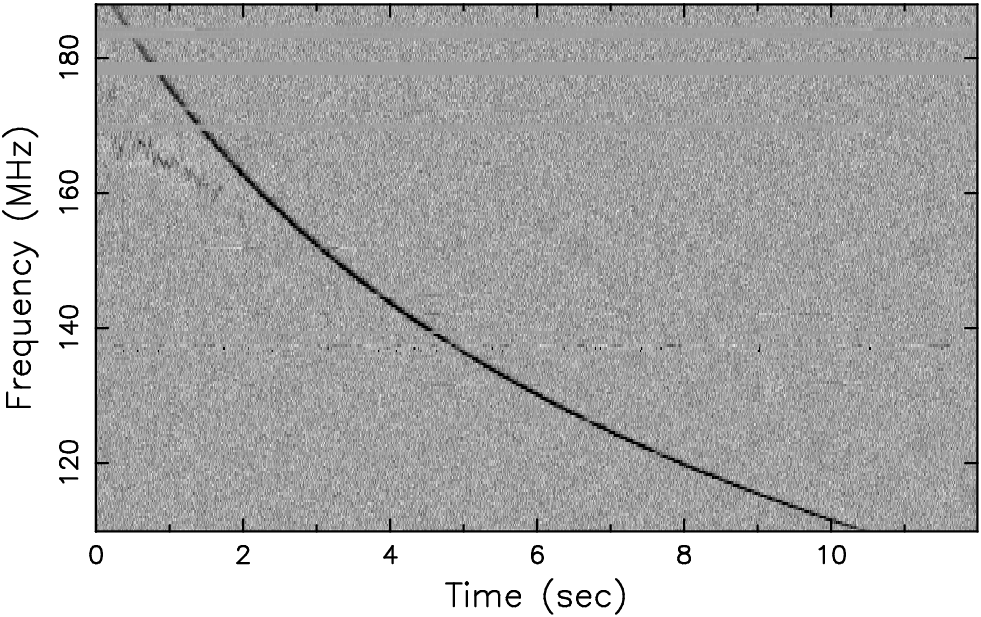
\includegraphics[width=0.6\textwidth]{Figures/Introduction/dispersed_data_2}
    \caption[The effect of dispersion on a pulse profile]{An illustration of the effect of dispersion on an observation of PSR~J0250+5854, which has a DM of 45.3~cm$^{-3}$~pc (see Chapter~\ref{chapt: J0250}). Lower frequencies arrive later than higher frequencies, giving the spectrum a characteristic sweep. Fitting the pulse arrival times as a function of frequency is used to find the DM through Eq.~\eqref{eq: intro - dispersive delay}.}
    \label{fig: intro - DM illustration} 
\end{figure}




\subsubsection{Scattering}
\label{sec: intro - observation processing - ISM effects - scattering}

Both scattering and scintillation are effects caused by inhomogeneities in the ISM. Scintillation causes frequency-dependent intensity variations of the source over time -- a familiar example of scintillation is the twinkling of stars, which is caused by turbulence in the atmosphere. Scattering is related to scintillation -- regions of different (electron) density in the ISM will refract emission, causing different rays to follow slightly different paths to an observer. These paths will have different lengths, and hence this results in a distribution of arrival times for a given pulse. The effect of this is to cause the pulse profile to broaden, forming a scattering tail.

The shape of a pulse due to scattering can be treated as the convolution of the intrinsic profile shape with a one-sided, exponential decay function of the form $\exp{(-t/\tau_\mathrm{s})}$ where $t$ is time and $\tau_\mathrm{s}$ is the characteristic scattering timescale \citep{Sxxx1968}. The scattering timescale is a frequency-dependent power law, i.e. $\tau_\mathrm{s} \propto \nu^{-\alpha}$, and the index $\alpha$ depends on the scattering model assumed. A commonly applied model is the `thin screen' model which treats all scattering as arising from a narrow region positioned half way between the pulsar and the observer \citep[e.g.][]{Sxxx1968, Wxxx1972}. This gives $4 < \alpha < 4.4$, where $\alpha = 4$ assumes Gaussian inhomogeneities \citep{Lxxx1971,LLxx1976} and $\alpha = 4.4$ assumes a Kolmogorov spectrum \citep{Rxxx1977,LRK+2015}. However, empirical fitting based on multi-frequency observations show that the scattering index varies across the pulsar population, spanning a range between 1.3 and 5.6 \citep{SDOx1980,LMG+2004, LDKK2013, LKKx2015, GKK+2017}. As well as frequency dependence, there is a correlation between the DM and $\tau_\mathrm{s}$ which has been shown to be broadly parabolic in log-log space \citep[e.g.][]{BCC+2004,GKK+2017,IJWx2019}. This is likely due to the fact that pulsars with a higher DM are more distant, and hence their emission propagates through a greater depth of turbulent ISM. Overall, these relations imply that scatter broadening will be more significant at lower frequencies, and will more strongly affect distant pulsars with a higher DM.


\subsubsection{Faraday rotation}
\label{sec: intro - observation processing - ISM effects - faraday rotation}

A further frequency-dependent effect is Faraday rotation, which causes a change in the PA of linear polarisation of a signal. This can be described by a rotation in the $Q-U$ plane of the Poincar\'e sphere, determined by comparing the left- and right-handed circular polarisations of a beam of light. Compared to a wave of infinite frequency, the wave with frequency $\nu$ lags in phase $\Psi$ by
\begin{equation}
    \label{eq: intro - faraday rotation angle}
	\Delta\Psi_\mathrm{Faraday} = \int^d_0 (k_\mathrm{R}-k_\mathrm{L})\ \mathrm{d}l,
\end{equation}
where $k_\mathrm{R}$ and $k_\mathrm{L}$ are the wavenumbers of right- and left-handed circularly polarised light, and the integral is along the line of sight. Faraday rotation takes place in a cold, magnetised plasma with a wavenumber
\begin{equation}
    \label{eq: intro - magnetised plasma wavenumber}
    k(\nu) = \frac{2\pi}{c}\nu \sqrt{1-\bigg(\frac{\nu_\mathrm{p}}{\nu}\bigg)^2 \pm \frac{\nu_\mathrm{p}^2\nu_\mathrm{B}}{\nu^3} }.
\end{equation}
It can be seen that different directions of circularly polarised light propagate at different speeds: right-handed (`$+$') circularly polarised light travels faster than left-handed (`$-$') polarised light when $B_\parallel$ is positive, and vice versa when it is negative.
In Eq.~\eqref{eq: intro - magnetised plasma wavenumber} $\nu_\mathrm{B}$ is the cyclotron frequency which is governed by the strength of the Galactic magnetic field $B_\parallel$ along the line of sight,
\begin{equation}
    \label{eq: intro - cyclotron frequency}
	\nu_\mathrm{B} = \frac{eB_\parallel}{2\pi m_\mathrm{e}c}.
\end{equation}
In this relation $e$ and $m_\mathrm{e}$ are the electron charge and mass respectively. 

The change in the observed position angle PA, $\psi$, by Faraday rotation is half the induced phase difference between the two circular polarisations, $\Delta\Psi_\mathrm{Faraday}$, and can be expressed in terms of the \textit{rotation measure} RM:
\begin{equation}
    \label{eq: intro - PA rotation angle}
	\Delta\psi_\mathrm{PA} = \frac{1}{2} \Delta\Psi_\mathrm{Faraday} \equiv \mathrm{RM} \times \lambda^2.
\end{equation}
In a similar manner to the dispersion measure (Eq.~\eqref{eq: intro - dispersion measure definition}), the rotation measure is defined by
\begin{equation}
    \label{eq: intro - rotation measure definition}
	\mathrm{RM} = \frac{e^3}{2\pi m_\mathrm{e}^2 c^4} \int^d_0 n_\mathrm{e}B_\parallel\ \mathrm{d}l.
\end{equation}

Faraday rotation manifests itself as a frequency-dependent rotation of the PA as illustrated in Fig.~\ref{fig: intro - RM illustration}.
\begin{figure}
	\centering
	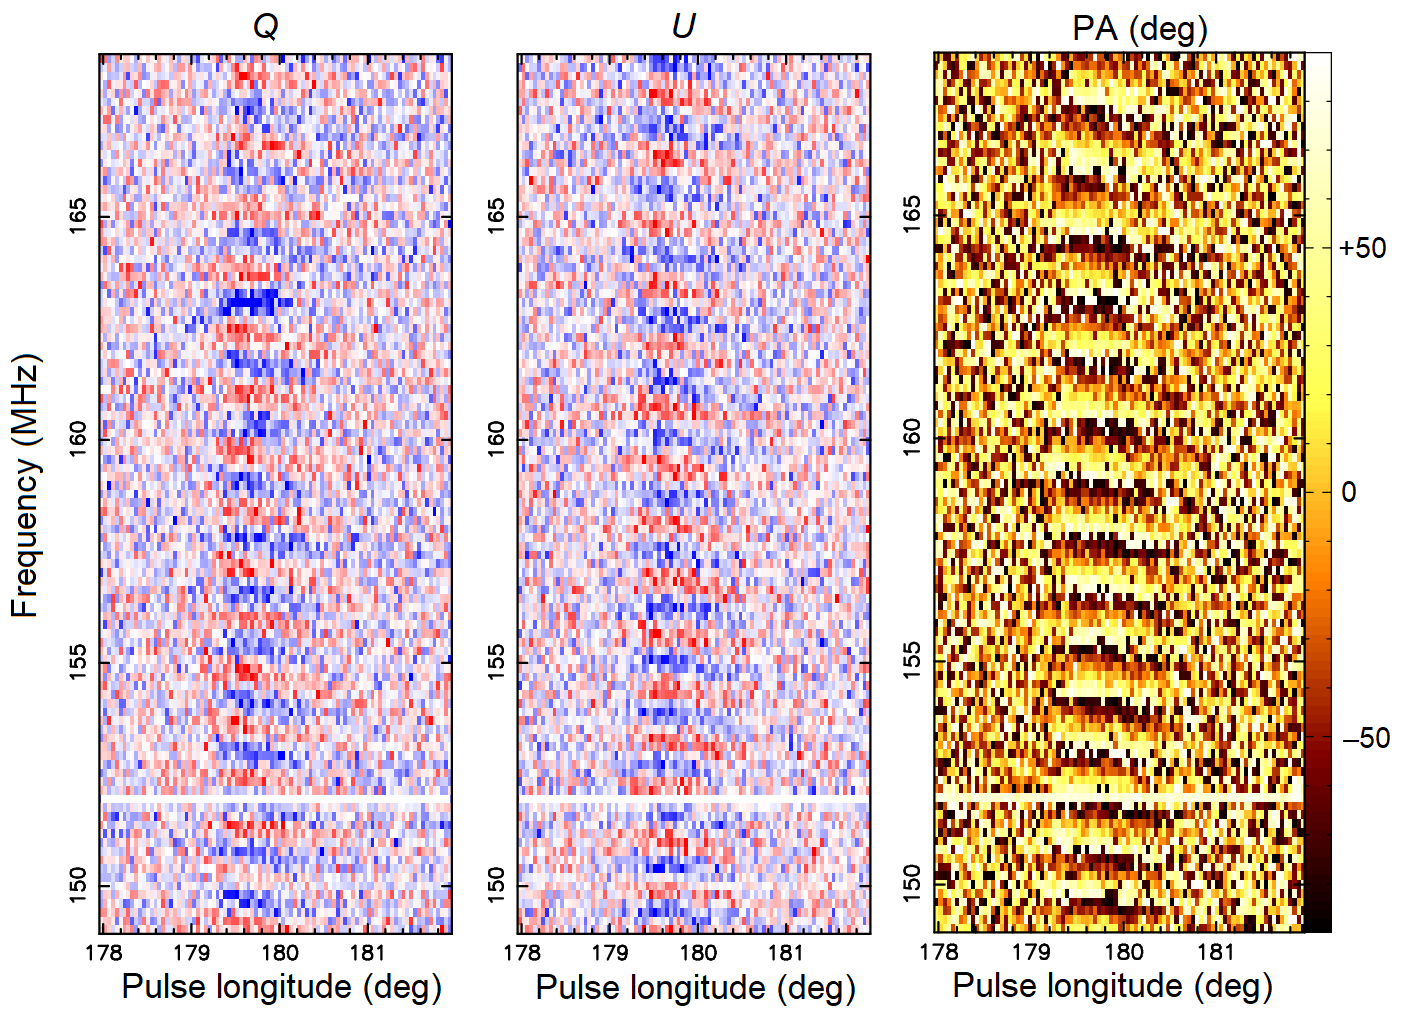
\includegraphics[width=0.8\textwidth]{Figures/Introduction/RM_data}
    \caption[The effect of Faraday rotation on polarisation]{An illustration of the effect of Faraday rotation on a polarised observation of PSR~J0250+5854, which has a RM of $-54.7$~rad~m$^{-2}$ (see Chapter~\ref{chapt: J0250}). There is a frequency-dependent rotation of the PA which is stronger at lower frequencies. In Stokes $Q$ and $U$ this manifests as a variation between positive and negative values which can lead to apparent depolarisation if one sums over the frequency channels.}
    \label{fig: intro - RM illustration} 
\end{figure}
If uncorrected for it can lead to depolarisation if the frequency channels are summed over, meaning the linear polarisation will be underestimated and the sensitivity of the average PA curve significantly reduced. De-Faraday rotation is the process of computing $\Delta\psi_\mathrm{PA}$ for each frequency channel according to Eq.~\eqref{eq: intro - PA rotation angle}, and then subtracting this phase from Stokes $Q$ and $U$. This requires the RM to be known.

% A method to determine the RM in pulsar astronomy is the Fourier-based RM synthesis technique \citep{Bxxx1966, BBxx2005}, used to calculate the RM of PSR~J0250+5854 in Chapter~\ref{chapt: J0250} for example.
% This method is based on calculating the RM power spectrum, $|F(\mathrm{RM})|^2$, using a discrete Fourier transform where 
% \begin{equation}
%     F(\mathrm{RM}) = K \sum_{j=1}^N P_j e^{-2i \mathrm{RM} (\lambda^2_j - \lambda^2_0)}.
% \end{equation}
% Here $K$ is a normalisation constant, $j$ is the frequency channel number (of which there are $N$), $P_j = Q_j + iU_j$ is the linear polarisation vector expressed as a complex number, $\lambda_j$ is the wavelength of channel $j$, and $\lambda_0$ is a reference wavelength (see \citealt{Hxxx2008} for further details). The RM power spectrum, $|F(\mathrm{RM})|^2$, which effectively quantifies the linear polarisation fraction as a function of trial RM, will peak at the RM of the pulsar. The power spectrum is usually taken to be the average across the pulse profile, however calculating the longitude-resolved RM can reveal slight deviations from the mean which point to magnetospheric effects taking place in the pulsar magnetosphere \citep{IJWx2019}.

By de-Faraday rotating the data, the sum of the linear polarisation across all frequency channels is maximised. Each frequency channel is rotated according to Eq.~\eqref{eq: intro - PA rotation angle}. The total linear polarisation is then effectively, 
\begin{equation}
    \label{eq: intro - defaraday rotation}
    L_\mathrm{integrated} = \sum_{j=1}^N P_j e^{-2i \mathrm{RM} (\lambda^2_j - \lambda^2_0)}.
\end{equation}
Here $j$ is the frequency channel number (of which there are $N$), $P_j = Q_j + iU_j$ is the linear polarisation vector expressed as a complex number, $\lambda_j$ is the wavelength of channel $j$, and $\lambda_0$ is a reference wavelength. This is essentially a discrete Fourier transform (if the wavelengths $\lambda_j$ are evenly spaced), and is the basis of the RM synthesis technique \citep{Bxxx1966, BBxx2005, Hxxx2008} which can be used to determine the RM of a pulsar by finding RM that corresponds to the peak of the $L_\mathrm{integrated}$ power spectrum. This was the method used to determine the RM of PSR~J0250+5854 in Chapter~\ref{chapt: J0250}.
















\section{Thesis outline}
\label{sec: intro - thesis outline}

This thesis focuses on two fields: investigations into the polarisation properties of radio pulsars, and the variability and systematic modulation of their individual pulses. The structure of the rest of this thesis is as follows.

Chapter~\ref{chapt: B0031} is an examination of the complex single-pulse polarisation behaviour of PSR~B0031$-$07, which exhibits both drifting subpulses and intensity-modulated orthogonal polarisation transitions. The complicated asymmetry in the drift modes is attributed to magnetospheric mixing of the OPMs, whilst the drifting subpulses are believed to originate from a carousel structure. This circulating carousel is mapped for the two drift modes observed and a model for the mixing of the OPMs is investigated.

Chapter~\ref{chapt: J1926} presents an investigation into PSR~J1926$-$0652, a pulsar with interesting single-pulse modulation properties discovered by the Five-hundred-metre Aperture Spherical radio Telescope (FAST). Some of these results were published in \citet{ZLH+2019}. Polarised data from Parkes are also analysed in order to constrain the geometry of this pulsar. Alongside drifting subpulses, PSR~J1926$-$0652 shows frequent nulling, and strong evidence of a connection between the two mechanisms is found, with highly significant differences in the emission immediately prior to a null.

In Chapter~\ref{chapt: J1518} I present analysis of PSR~J1518+4904, which was observed four times with FAST in 2018 in order to study `jitter noise', stochastic variations in the profile shape on a pulse-to-pulse basis. Through Fourier analysis this pulsar was revealed to show very unusual single-pulse modulation, with multiple discrete $P_3$ periodicities present simultaneously at different pulse longitudes. A continuous, longitude dependence of $P_3$ was also observed for one of the profile components, which poses hard questions for current single-pulse modulation models.

Chapter~\ref{chapt: J0250} covers observations of the slowest known pulsar PSR~J0250+5854 \citep[$P_1 = 23.5$~s, ][]{TBC+2018} performed simultaneously with FAST and three Low Frequency Array (LOFAR) international stations. This new data increases the spectral coverage of this pulsar five-fold, and reveals that it has a steep spectrum with a low-frequency turnover. The profile is shown to broaden at higher frequencies, counter to expectations from radius to frequency mapping \citep[e.g.][]{KGxx2003}. Comparisons are drawn between this radio pulsar and the magnetars. This work is currently under review with Monthly Notices of the Royal Astronomical Society.


Finally, Chapter~\ref{chapt: conclusions} presents the conclusions of this work, including a summary of the remaining questions and suggestions for the potential direction of further research.
\chapter[Complex pulsar polarisation and its implications]{Complex radio polarisation variability in PSR B0031$-$07 and the implications for its magnetosphere}
\label{chapt: B0031}

I present a model to explain the curious intensity-modulated orthogonal polarisation mode (OPM) transitions of PSR~B0031$-$07. This pulsar exhibits drifting subpulses where the position angle of the emission suddenly changes within a single pulse, also from one pulse to the next, and is linked to the drifting subpulses seen in total intensity. This poses significant problems for the carousel model which is used to explain drifting subpulses, as the sub-beams appear to be changing their properties as they circulate. I propose that the observed asymmetries in both the polarisation properties and total intensity may be caused by coupling of the two OPMs as they propagate through the magnetosphere. As well as being attenuated, power is allowed to be transferred between them, and this occurs in an asymmetric, pulse longitude-dependent fashion, and is parametrised by a `mixing matrix'. I show that this implies that the underlying mechanism responsible for the drifting subpulses could be symmetric, as predicted by the carousel model. An image of the polar emission region compatible with the observations is found. An atlas of different geometrical parameters is explored, and the form of the mixing matrix is shown to be independent of the assumed geometrical parameters which determine the structure of the carousel. The difference in the mixing matrix between the two drift modes is seen as evidence for a global reconfiguration of the magnetosphere when mode-switching takes place.

\section{Introduction}
\label{sec: B0031 - introduction}

Although it has been more than half a century since the discovery of pulsars \citep{HBP+1968}, explaining the multitude of observational phenomenology still remains challenging. A good example is the peculiar polarisation behaviour of PSR~B0031$-$07 \citep{IWJ+2020} which exhibits orthogonal polarisation modes which switch periodically at a single-pulse level synchronously with the drifting subpulses seen in total intensity. This behaviour will be studied in more detail here with the aim to provide an interpretation. Two key features of radio pulsar emission are of interest in this discussion: drifting subpulses, whereby individual pulses drift across the pulse window at a steady rate; and position angle (PA) jumps which are associated with the presence of two orthogonal polarisation modes (OPMs) of emission.

In at least 55~per~cent of radio pulsars \citep{WESx2007} drifting subpulses occur. First noted by \citet{DCxx1968} in PSR~B1919+21, these drifting subpulses can be characterised by two quantities: the spacing between them in rotational phase, $P_2$, and the number of stellar rotations it takes for the pattern of subpulses to repeat itself, $P_3$ \citep{SSPW1970}. When single-pulse data is presented as a `pulse stack', drifting subpulses give rise to the appearance of `driftbands', diagonal bands of intensity. The carousel model \citep{RSxx1975} is an often-invoked, although still controversial, model for the beam structure that gives rise to drifting subpulses. In this model the radio beam is composed of multiple sub-beams in a ring-like configuration which circulate around the magnetic axis with a period $P_4$, fed by `sparks' close to the surface of the star. The steady circulation gives the appearance of drifting subpulses for the observer, as illustrated in Fig.~\ref{fig: intro - driftband schematic}. In general a given sub-beam will intercept the line of sight (LOS) to the observer at two separate pulse longitudes (i.e. rotational phases of the star), appearing once in the leading half of the profile and once in the trailing half when the carousel is rotated further. Under the assumption that the sub-beams are not changing in shape, or only change stochastically while circulating, one expects symmetrical integrated pulse profiles. However, in reality most pulsars have profiles which are distinctly asymmetric. This suggests that other effects need to be considered, such as the propagation of the radiation through the pulsar magnetosphere.

Another important feature of radio pulsar emission is its polarisation. As explained in Sec.~\ref{sec: intro - emission models - polarisation}, pulsar emission typically has a high degree of polarisation, especially in younger pulsars \citep[e.g.][]{GLxx1995}. The orientation of the linear polarisation vector on the sky, i.e. PA, is observed to be pulse longitude-dependent. For some pulsars this takes the form of a smooth, monotonic, S-shaped curve -- this can be explained by the changing orientation of the magnetic field with respect to the LOS, and is described by the Rotating Vector Model \citep[RVM;][see Sec.~\ref{sec: intro - emission models - polarisation - RVM}]{RCxx1969,Kxxx1970}. Other pulsars show a rapid change of $\sim$90$\degr$ in PA at some pulse longitudes. This is a manifestation of the presence of two (nearly) orthogonal emission modes which change in relative intensity across the pulse profile \citep[e.g.][]{RCBx1974,BRCx1976}. The origin of OPMs is described in Sec.~\ref{sec: intro - emission models - polarisation - OPMs}. %A possible explanation for the origin of OPMs was given by \citet{Mxxx1979} and \citet{ABxx1986}, who proposed that the distinct modes are associated with the natural propagation modes in the pulsar magnetosphere. In an ultra-relativistic plasma, radiation can propagate via two modes; the `ordinary' (O-) and the `extraordinary' (X-) modes. In a strong magnetic field such as is found in pulsar magnetospheres, the X-mode decouples from the plasma and propagates freely. However, the O-mode remains coupled to the plasma and is therefore subject to refraction. The result is that the X-mode emission follows a straight path whereas the path followed by the O-mode is curved. Although they may originate from the same place, the difference in path means that the two modes are no longer observed simultaneously, giving the impression of pulse longitude-dependent changes in the intensity of the modes. This can lead to OPM jumps and asymmetry of the (polarised) pulse profile.

The carousel model, as proposed by \citet{RSxx1975}, only considers total intensity; Stokes $I$ -- it needs to be modified in some way to account for polarisation, and work in this area has been done by \citet{RRS+2002} and \citet{RRL+2006} to explain the variable pulse-to-pulse polarisation properties of PSR~B0809+74. \citet{RRS+2002} showed that the dominating OPM observed in this pulsar periodically switches during the subpulse modulation cycle. In its pulse stack, one OPM traces the total intensity driftbands, whilst the other was found to dominate in between the driftbands. \citet{RRL+2006} interpreted this in terms of the carousel model by exploiting the cartographic transforms as defined by \citet{DRxx2001}, which allows mapping of the beam structure surrounding the magnetic pole. They showed that the circulating radiation pattern as observed for one of the OPMs is extended further out from the magnetic axis, and is out of phase such that it falls in between the sub-beams observed for the other OPM.

Even more complex single-pulse polarisation behaviour is reported for PSR~B0031$-$07 as observed at a centre frequency of 1369~MHz with the Parkes telescope \citep{IWJ+2020}. For this pulsar the drifting subpulse pattern is relatively variable, so the technique of $P_3$-folding was used \citep{HSW+2013,Wxxx2016}. In this method, the pulses were folded at the period $P_3$ after correcting for the variability in the repetition rate of the pattern, as explained in Sec.~\ref{sec: intro - emission models - single pulse phenomena - P3 folding}. This allows the structure and polarisation of the average driftband to be studied with a much higher signal-to-noise ratio than achievable for individual pulses. PSR~B0031$-$07 has two distinct modes of drifting subpulses at this frequency, $P_3 = 12.85 P_1$ (drift mode A) and $P_3 = 6.87 P_1$ (drift mode B). Here $P_1$ is the pulse period, which is 0.943 seconds.

\begin{figure}
    \begin{center}
        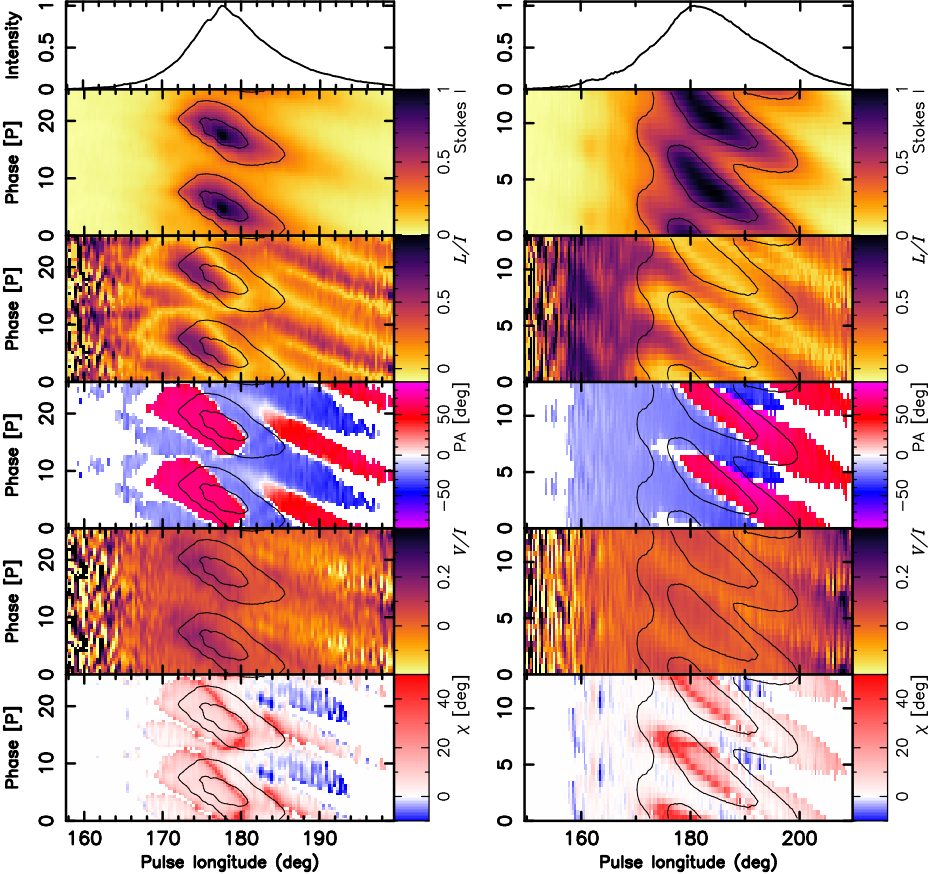
\includegraphics[width=1.0\textwidth]{Figures/B0031/observed_P3folds}
        \caption[The two P3-folded drift modes of PSR~B0031$-$07]{The two drift modes of PSR~B0031$-$07 folded at the period $P_3$. Mode A is shown in the left-hand column and mode B on the right. The total intensity driftbands are shown at the top, under the pulse profile. In descending order, the five colour plots are Stokes $I$, linear polarisation fraction $L/I$, PA, circular polarisation fraction $V/I$, and ellipticity angle $\chi$. The $P_3$ cycle is plotted twice for clarity, and the total intensity driftband is shown by the contour plots in the lower four plots of each mode. Figure recreated with permission from \citet{IWJ+2020}.}
        \label{fig: B0031 - observed P3folds}
    \end{center}
\end{figure}

The $P_3$-folds of both drift modes are shown in Fig.~\ref{fig: B0031 - observed P3folds} and reveal that the A (left-hand panels) and B (right-hand panels) drift patterns of PSR~B0031$-$07 are very different. In total intensity (top panels) pattern A exhibits bright, concentrated emission in the leading half of the driftbands followed by a much fainter and gradually dimming tail, whereas pattern B has a wider and somewhat more symmetrical pattern. Both seem to show a bend in the driftband at around pulse longitude $\phi = 185\degr$, after which the band becomes more shallow. There is also evidence in pattern B for another small patch of modulated emission preceding the main driftband at pulse longitude $162\degr$, which is not present in pattern A. Even more complex are the position angle patterns (fourth row of panels in Fig.~\ref{fig: B0031 - observed P3folds}). For mode B only the trailing half of the profile shows periodic changes in PA, such that the OPM with a positive PA (represented by the red colouring) roughly traces the Stokes $I$ driftbands (indicated by the contours). This association of one OPM with the total intensity pattern resembles the behaviour of PSR~B0809+74 \citep{RRS+2002}. In mode A also the leading half of the pulse shows periodic modulation of the dominating OPM. For the leading half of the profile the OPM with a positive PA is mostly associated with the driftbands as seen in total intensity, while at $\phi \sim 180\degr$ the two OPMs seem to abruptly switch.

PSR~B0031$-$07 is not unique in showing OPM variability associated with drifting subpulses: other than PSR~B0809+74 \citep{ESxx2004,RRL+2006} periodic OPM switches have also been identified in PSR~B0320+39 and B0818$-$13 \citep{ESxx2004}, and PSR~B1237+25 \citep{RRxx2003}. In these pulsars the Stokes $I$ driftbands are dominated by one OPM with the other OPM occurring in between, whereas for drift mode A of PSR~B0031$-$07, the OPMs appear to switch {\it within} the Stokes $I$ driftband in the pulse longitude direction. This switching is problematic in the sense that it means that these observations cannot be explained by a static pattern of OPMs circulating the magnetic axis, the picture used to explain the observations of PSR~B0809+74. The aim of this work is to see if the polarised subpulse pattern of PSR~B0031$-$07 can be explained within the framework of the carousel model. The possibility that magnetospheric propagation effects are responsible for the asymmetric pattern observed in the PA $P_3$-fold is explored. Although asymmetric refraction cannot be ruled out, it is hard to model mathematically without any specific model that predicts the functional shape of refraction throughout the magnetosphere. A simpler model with many fewer degrees of freedom would be to consider that the two OPMs remain coupled during propagation through the magnetosphere \citep[e.g.][]{Pxxx2001}. In this context coupling means that power can be exchanged between the two modes; in addition, the OPMs may be attenuated, reducing the overall intensity. I suggest that the asymmetries observed arise from these longitude-dependent processes. It will be demonstrated that these processes cannot be uniquely constrained. Nevertheless, it will be found that solutions do exist that describe the observations in terms of a static, circulating pattern of sub-beams in line with the prediction of a carousel model.

The following sections will explain how the observed polarised intensity is separated into the intensity of two OPMs. The cartographic transforms of \citet{DRxx2001} are discussed along with the symmetry predicted by the carousel model. The cartographic transform cannot be used directly to map the circulating system of polarised sub-beams, as the magnetospheric distortions need to be considered -- the mathematical description used to quantify these distortions will be defined, as well as how they can be used to show that a static circulating pattern of polarised sub-beams can explain the asymmetric pattern of PA in both drift modes of PSR~B0031$-$07.



%%%%%%%%%%%%%%%%%%%%%%%%%%%%%%%%%%%%%%%%%%%%%%%%%%%%%%%%%%%%%%%%%%%%%%%%%%%%%%%%%%%%%%%%%%%%%%%%%
%%%%%%%%%%%%%%%%%%%%%%%%%%%%%%%%%%%%%%%%%%%%%%%%%%%%%%%%%%%%%%%%%%%%%%%%%%%%%%%%%%%%%%%%%%%%%%%%%




\section{Methods}
\label{sec: B0031 - methods}

\subsection{Magnetospheric distortions}
\label{sec: B0031 - methods - magnetospheric distortions}

It is known \citep[e.g.][]{ABxx1986,BAxx1986,Pxxx2000} that refraction can cause a spatial separation of the two OPMs, which originate from a common source. This spatial separation has been suggested as the reason for the presence of OPM transitions (e.g. \citealt{ESLx2003,ESxx2004}). Refraction is due to plasma density gradients in the magnetosphere. This plasma density is believed to have minima at both the magnetic pole and the boundary of the open-field-line region \citep[e.g.][]{LPxx1998}, and this was used by \citet{PLxx2000} to demonstrate how emission produced relatively close to the magnetic axis could be refracted inwards to the other side of the magnetic axis, whilst emission further out is refracted even further outwards. This pole crossing means that an observer may simultaneously receive emission which originated from either side of the magnetic axis. This effect can lead to the appearance of nested cones from a single carousel. In an axisymmetric plasma distribution, any refraction occurs entirely in the plane of the magnetic field lines. If the carousel consists of an odd number of sub-beams, then emission from a sub-beam that is refracted (O-mode) across the pole ought to be out of phase relative to the emission of the non-refracted (X-mode) sub-beam component. When refractive delays or retardation effects are considered \citep{ESLx2003}, the sub-beams might not appear exactly out of phase. Larger azimuthal offsets could be caused by symmetry-breaking by magnetospheric rotation, or a non-axisymmetric plasma distribution \citep{BCWx1991, PLxx2000}. This is potentially a good description for what has been observed for PSR~B0809+74 \citep{RRL+2006}.

In mode A of PSR~B0031$-$07, the position angle (PA) of linear polarisation undergoes an OPM transition \textit{within} a given total intensity driftband such that the Stokes $I$ driftband is associated with different OPMs at different pulse longitudes (see Fig.~\ref{fig: B0031 - observed P3folds}). This change implies that the perceived polarisation properties of a given sub-beam have changed as it circulates, so that the emission from one OPM dominates at later longitudes whilst the other becomes stronger as the sub-beam drifts to earlier longitudes. This observation, as shown in the $P_3$-fold, is reproducible over long timescales. This suggests that a propagation effect is responsible. The required asymmetry with rotational phase of the pulsar is potentially caused by anisotropies in the magnetosphere at altitudes much higher, and over larger scales, than the emission region. Although refraction could play a role in causing the observed asymmetries, it is hard to model mathematically with a small number of parameters without any specific model to predict the functional shape of the refraction throughout the magnetosphere. In the absence of such a refraction model it would be impossible to construct the underlying, undistorted map of how the sub-beam structure of the carousel appeared before being affected in this way.


A much more tractable, and arguably more intuitive alternative model for longitude-dependent asymmetry is coupling of the OPMs in such a way that power can be transferred between them as they travel, as illustrated in Fig.~\ref{fig: B0031 - coupling schematic}.
\begin{figure}
    \begin{center}
        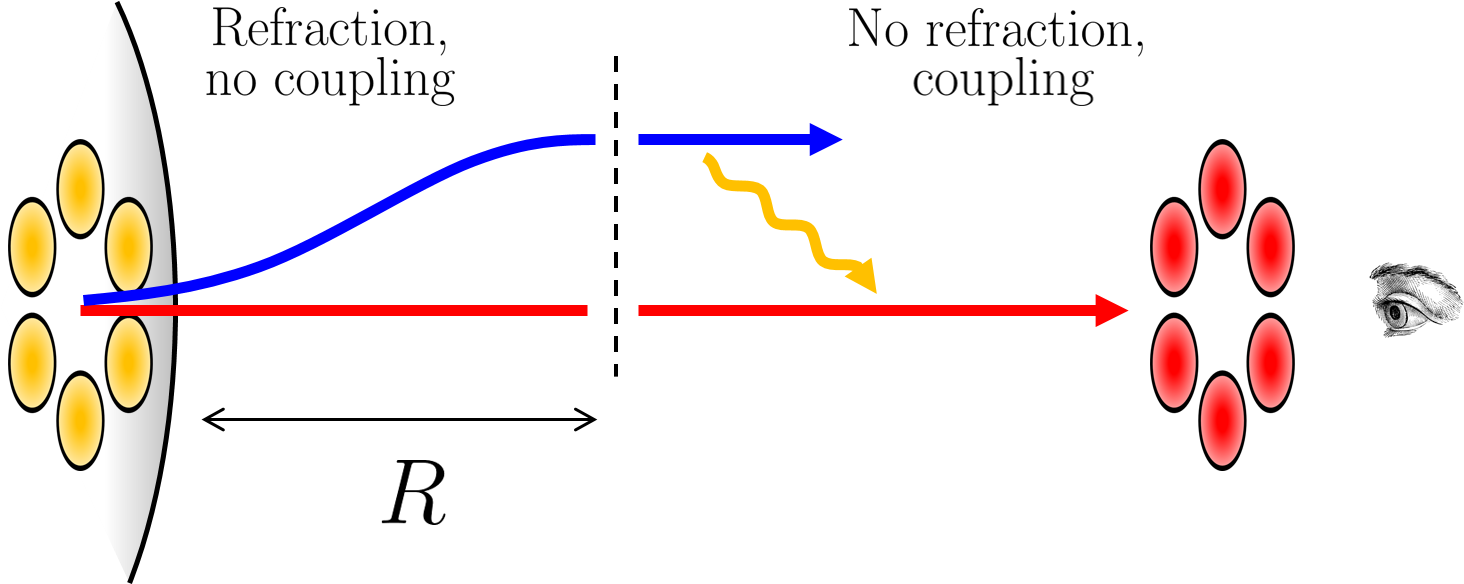
\includegraphics[width=0.7\textwidth]{Figures/B0031/coupling_schematic2}
        \caption[Schematic view of propagation of two OPMs through the magnetosphere]{A schematic representation of how refraction and mode coupling may occur in the pulsar magnetosphere. Two OPMs are generated at a common source, and propagate upwards. Below some radius $R$ refraction is the dominant effect, with the O-mode (blue) being refracted whilst the X-mode (red) travels freely. Above the limiting radius, refraction is no longer significant, whilst coupling becomes dominant. Power is allowed to be transferred between the two OPMs, and an observer sees the PA of the dominant OPM.}
        \label{fig: B0031 - coupling schematic}
    \end{center}
\end{figure}
Below some radius $R$, the propagation of the two OPMs is refraction-dominated: they originate from a common source, but the OPM identified with the O-mode is subject to refraction (blue in the figure), whereas the X-mode (red) is not \citep{ABxx1986}. The modes are not coupled in this region. At altitudes greater than $R$ refraction no longer plays an important role and coupling of the two modes becomes a strong effect. Any offset of the emission patterns due to refraction becomes `baked in', and the only further changes to the OPMs are due to the transfer of power between them and attenuation.
The idea of mode coupling is not new. \citet{Pxxx2000} suggested that refraction dominates only at low altitudes where the plasma density is sufficiently high. As the OPMs propagate outwards they enter a region where power may be transferred between the O- and X-modes. This conversion happens up to a certain height, after which the rays propagate independently again (unaffected by coupling or refraction). This model is discussed further in Sec.~\ref{sec: B0031 - discuss - general discusison}.
The assumption made in this work is that the observed asymmetry of PSR~B0031$-$07 is dominated by what happens above $R$. In that case there is a rotationally symmetric sub-beam structure produced by the carousel, possibly distorted (symmetrically) by refraction. The aim of this chapter is to deduce this maybe distorted, but overall axisymmetric, sub-beam structure from the observations.

This intrinsic beam structure circulates and would produce symmetrical driftbands and profile shapes. However, the modes are permitted to couple in a way which allows the modes to be mixed and attenuated above $R$. This transformation can be expressed by the simple matrix equation,
\begin{equation}
\label{eq: definition of the mixing matrix}
    \mathbf{O} = \begin{pmatrix} O_1\\O_2 \end{pmatrix} = \begin{pmatrix} M_{11} & M_{12}\\M_{21} & M_{22} \end{pmatrix} \begin{pmatrix} I_1\\I_2 \end{pmatrix} = \mathbf{MI},
\end{equation}
where $O_1$ and $O_2$ are the intensities of the observed OPMs (at a given pulse longitude and pulse number), $I_1$ and $I_2$ are the intensities of the `intrinsic' OPMs (i.e. before being affected by mode coupling), and $\mathbf{M}$ is the `mixing matrix' that parametrises the coupling and attenuation of the OPMs due to propagation through the magnetosphere. Absorption effects have been cited as the cause of asymmetric profiles \citep[e.g.][]{Rxxx1983b}, and this effect would correspond to the diagonal elements of $\mathbf{M}$. Mode coupling, including non-zero off-diagonal terms, can be seen as a generalisation of this concept.

In this model, the observed asymmetry is a consequence of the pulse longitude-dependence of the mixing matrix, which is otherwise taken to be independent of time during the modulation cycle. So there exists an intrinsic pattern of sub-beams (describing $I_1$ and $I_2$) that is static in the sense that their structure and polarisation properties are time-invariant apart from their circulation, and all asymmetry in the driftbands and profile is caused by mode coupling. The `intrinsic' driftbands (and hence carousels) to be recovered are the patterns of radiation seen after refraction has taken place, so some azimuthal and radial offset of the two OPM sub-beams can be expected. Under these assumptions, the mixing model should be able to reproduce the observed $P_3$-folds. Since the $P_3$-fold technique has effectively averaged many different beamlets, it is the average beam structure which will be described by the model, thereby ignoring additional stochastic variability. The symmetry of the circulating intrinsic intensity pattern can be exploited (at least up to some level) to isolate and remove the distortions caused by mode coupling -- to do this, we first separate the observed emission into the two observed OPMs, $O_1$ and $O_2$.

%%%%%%%%%%%%%%%%%%%%%%%%%%%%%%%%%%%%%%%%%%%%%%%%%%%%%%%%%%%%%%%%%%%%%%%%%%%%%%%%%%%%%%%%%%%%%%%%%
%%%%%%%%%%%%%%%%%%%%%%%%%%%%%%%%%%%%%%%%%%%%%%%%%%%%%%%%%%%%%%%%%%%%%%%%%%%%%%%%%%%%%%%%%%%%%%%%%






\subsection{Separating the OPMs}
\label{sec: B0031 - methods - mode separation}

To split the observed emission into the intensities of the two OPMs $O_1$ and $O_2$, the position angle (PA) and the linear polarisation fraction $L/I$ are taken into account at each point in the $P_3$-fold. Orthogonally polarised modes are in general thought to have PAs which differ by $90\degr$, and have equal but opposite ellipticities. They are therefore antipodal when represented on a Poincar\'e sphere. The expected signature of an OPM transition in a pulse profile is that when a PA jump occurs both the linear and circular polarisation fractions go to zero (complete depolarisation). However, for PSR~B0031$-$07 \citet{IWJ+2020} found that while the two modes are offset by $90\degr$ in PA, only one of the modes appears to have circular polarisation associated with it -- strictly speaking then the modes are non-orthogonal. The separation of non-orthogonal polarisation modes was explored by \citet{Mxxx2003} in the context of OPMs that are non-orthogonal in PA, highlighting that separating non-orthogonal OPMs is not possible without making additional assumptions to break the arising degeneracies. Further discussion of non-orthogonal modes can be found in Sec.~\ref{sec: B0031 - discussion}

The method used to split the observed emission into $O_1$ and $O_2$ is similar to that of \citet{MSxx2000} except that the circularly polarised intensity component was not considered. This is justified because throughout the profile the circularly polarised fraction is much weaker than the linear polarisation, as shown in the third ($L/I$) and fifth ($V/I$) rows of Fig.~\ref{fig: B0031 - observed P3folds}. The OPMs are assumed to combine incoherently to explain the observed unpolarised component of the radiation. Incoherent mode addition can readily explain the sudden PA jumps, while for coherent mode addition the PA transitions may be expected to be much smoother. This is discussed further in Sec.~\ref{sec: B0031 - discussion}. In the process of separating the OPMs in the $P_3$-fold, the Stokes parameters are rotated by the observed PA at a given longitude in the pulse profile which has the effect of removing any systematic pulse longitude-dependence of the PA caused by the Rotating Vector Model or otherwise. This means that these effects do not have to be considered in further analysis.

\begin{figure}
    \begin{center}
        \includegraphics[width=\textwidth]{Figures/B0031/observed_OPMs}
        \caption[PSR~B0031$-$07's two drift modes split into two OPMs]{The separated observed OPMs of the two drift modes, with drift mode A on the left and mode B on the right. The upper panel shows the integrated profiles of each OPM, normalised to the peak of the stronger of the two, with OPM 1 shown by the solid line and OPM 2 by the dashed line. The colour plots show the observed driftbands, with OPM 1 above and OPM 2 below. The mean pulse longitude-dependent intensity has been subtracted from these $P_3$-folds.}
        \label{fig: B0031 - observed OPMs}
    \end{center}
\end{figure}

Figure.~\ref{fig: B0031 - observed OPMs} shows the intensity of the separated observed OPMs for each drift mode, which are referred to as OPM 1 and OPM 2 respectively (the order is arbitrary). These $P_3$-folds have had the mean intensity subtracted from each pulse longitude column, so they do not show the full intensity pattern but rather the variation about the mean. This highlights the modulation pattern which should be reproduced by a circulating pattern of beamlets, on top of any unmodulated background emission. As described in Sec.~\ref{sec: B0031 - methods - calculating intrinsic emission} and Appendix~\ref{app: matrix maths - accounting for unmodulated emission}, subtracting the mean has the advantage that unmodulated emission is properly taken into account in the fitting process used to constrain the mixing matrix. 

OPM 1 of mode A (upper left panel) has a small blob of emission at the leading edge of the driftband at around $172\degr$ which is not present at the trailing edge; instead the driftband has a smooth tail. Similarly, OPM 2 (lower left panel) has concentrated emission in the leading half, but after pulse longitude $185\degr$ this fades out slowly in an extended tail. Mode B, shown in the right-hand panels of Fig.~\ref{fig: B0031 - observed OPMs}, is more complex than mode A, and extends across a larger longitude range. In OPM 1 (upper right panel), the observed  $P_3$-fold has a chequerboard-like structure in the leading half (up to $\sim$180$\degr$) before settling into stable continuous driftbands in the trailing half. OPM 2 (lower right panel) has a similar stable pattern which only becomes visible around $170\degr$ but extends past $200\degr$. These asymmetries will be exploited to find the distortions which will be quantified with the mixing matrix introduced in Sec.~\ref{sec: B0031 - methods - magnetospheric distortions}. From the shape of the observed driftbands predictions can be made about the form the mixing matrix must take: for example, the chequerboard pattern of mode B, OPM 2 may arise from two intrinsic modes which have symmetrical diagonal driftbands, offset from each other in pulse number. Mode conversion can make different intrinsic modes dominate at different longitude intervals in an observed OPM, thereby giving rise to such a chequerboard pattern.

In contrast, where the two observed OPM  $P_3$-folds have a very similar pattern, then one of the intrinsic modes may largely be suppressed, while the other is partially converted to the other observed mode. Such a scenario could be close to what is observed for the trailing half of mode B (right-hand panels of Fig.~\ref{fig: B0031 - observed OPMs}) after $\sim$185$\degr$, where the two OPMs appear very similar. In the following we will first quantify the expected symmetry for a circulating system of sub-beams. Any deviations from this should be explained with pulse longitude-dependent mode mixing.





%%%%%%%%%%%%%%%%%%%%%%%%%%%%%%%%%%%%%%%%%%%%%%%%%%%%%%%%%%%%%%%%%%%%%%%%%%%%%%%%%%%%%%%%%%%%%%%%%
%%%%%%%%%%%%%%%%%%%%%%%%%%%%%%%%%%%%%%%%%%%%%%%%%%%%%%%%%%%%%%%%%%%%%%%%%%%%%%%%%%%%%%%%%%%%%%%%%





\subsection{Carousel geometry}
\label{sec: B0031 - methods - carousel geometry}

During the rotation of the star, the orientation of the magnetic axis changes relative to the observer's line of sight (LOS). \citet{DRxx2001} defined a cartographic transform that maps the emission as recorded in a time series (i.e. a pulse stack and by extension a $P_3$-fold) onto a beam pattern relative to the magnetic axis. This allows an image of the radiation pattern to be constructed in a frame co-rotating with the carousel. The transform is defined by four parameters: the magnetic inclination angle, $\alpha$; the impact parameter of the LOS with respect to the magnetic axis, $\beta$; the period it takes for the carousel to complete one full circulation, $P_4$; and the pulse longitude corresponding to the fiducial plane, $\phi_\mathrm{fid}$. The fiducial plane is the plane in which the pulsar's magnetic and rotation axes lie. For an unaliased drifting subpulse pattern, the circulation period $P_4 \equiv NP_3$, where $P_3$ is the repetition period of the pattern in the pulse stack and $N$ is the number of sub-beams in the carousel. The transform used in this work is defined (Eqs.~\eqref{eq: cartographic transform - R}--\eqref{eq: cartographic transform - theta_rot}) and discussed in Appendix~\ref{app: geometry derivations}. This work extends the transform to include aliasing effects, which is discussed there too.

\begin{figure} [t]
	\begin{center}
	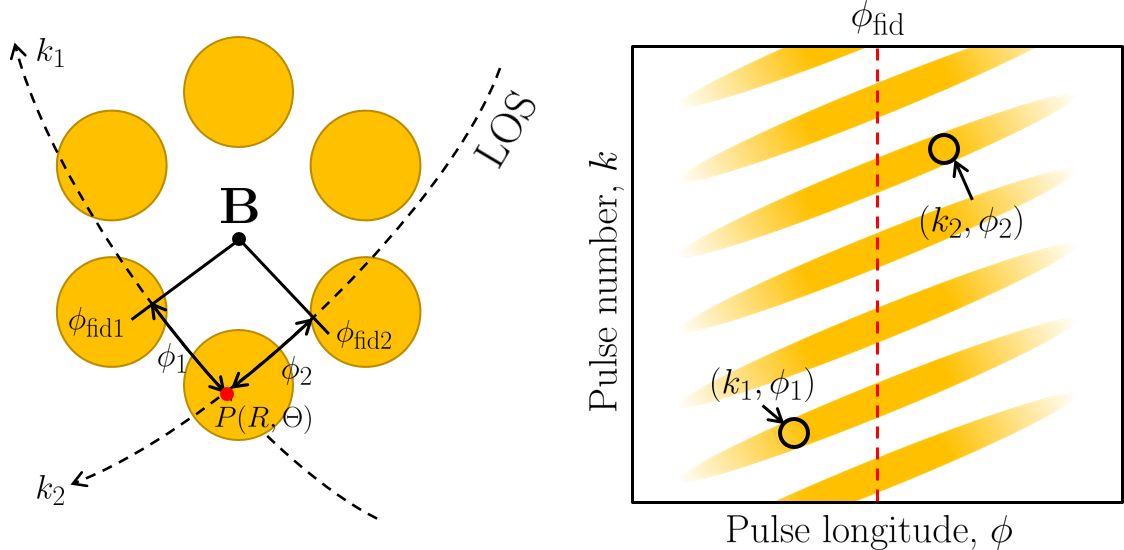
\includegraphics[width=0.9\textwidth]{Figures/B0031/opposite_points2}
	\caption[The predicted symmetry in driftbands arising from a circulating carousel]{An illustration of the argument that a carousel of sub-beams which remain unchanged during their circulation should produce `symmetric' pulse stacks such that two locations in the pulse stack have identical emission properties. LEFT: the carousel as viewed in a corotating frame. In this frame the line of sight appears to circulate, as is indicated for two stellar rotations $k_1$ and $k_2$. $\phi_\mathrm{fid 1,2}$ represents the location of the fiducial plane at each time. RIGHT: the pulse stack produced by such a carousel. The point $P$ intercepts the LOS at $k_1$ and $\phi_1$, and then the later at $k_2$ and $\phi_2$, so appearing in the pulse stack twice during a carousel rotation.}
    \label{fig: B0031 - symmetry}
    \end{center}
\end{figure}


As the carousel rotates, a given sub-beam will cross the observer's LOS twice, giving rise to an expected symmetry of the emission properties at two points on either side of the fiducial plane (see Fig.~\ref{fig: B0031 - symmetry}). In the left-hand panel a location in the carousel $(R, \Theta)$ -- labelled $P$ -- is intercepted by a LOS during the rotation number $k_1$ of the star at a longitude $\phi_1$. As the carousel circulates around the magnetic axis $(\vec{B})$, the point $P$ intercepts the LOS again at a later time (rotation $k_2$), this time at a different longitude $\phi_2$. This figure is drawn in a frame corotating with the carousel, so the carousel appears stationary while it is the LOS that moves. If the structure and intensity of the sub-beams do not change with time, the emission should be identical at points $(k_1,\ \phi_1)$ and $(k_2,\ \phi_2)$ in the pulse stack, shown on the right-hand side of Figure \ref{fig: B0031 - symmetry}. In folding the pulse stack at its modulation period $P_3$, the `average' driftband shape is found, meaning that the matching pair of points would be found in the same driftband. These points can be identified using the cartographic transform and methods explained in Appendix~\ref{app: geometry derivations - P3 fold - matching points}.

It should be noted that the transform used in this work, and the subsequent mathematics behind the argued symmetry of the drifting emission, is based on the assumption that the circulating carousel is perfectly circular. Elliptical carousels were proposed as an explanation for `bi-drifting' pulsars, where the subpulses move in opposite directions in different parts of the profile \citep{QLZ+2004, Wxxx2016, WWxx2017, SLWM2020}. This model still has an intrinsic symmetry, however it has more degrees of freedom and is significantly harder to describe mathematically. Therefore, in this work only simple, circular carousels are considered.





%%%%%%%%%%%%%%%%%%%%%%%%%%%%%%%%%%%%%%%%%%%%%%%%%%%%%%%%%%%%%%%%%%%%%%%%%%%%%%%%%%%%%%%%%%%%%%%%%
%%%%%%%%%%%%%%%%%%%%%%%%%%%%%%%%%%%%%%%%%%%%%%%%%%%%%%%%%%%%%%%%%%%%%%%%%%%%%%%%%%%%%%%%%%%%%%%%%






\subsection{Determining the intrinsic carousel emission}
\label{sec: B0031 - methods - calculating intrinsic emission}

As explained in Sec.~\ref{sec: B0031 - methods - carousel geometry}, the $P_3$-fold should obey an intrinsic symmetry with respect to the fiducial plane such that pairs of corresponding points can be identified in the $P_3$-fold (one in the leading half of the pulse and one in the trailing half). These pairs of points should intrinsically have the same (polarised) intensity. However, under the action of the mixing matrix (Eq.~\eqref{eq: definition of the mixing matrix}) differences can arise. To allow the polarisation to be intrinsically identical for the two points, Eq.~\eqref{eq: definition of the mixing matrix} can be used to link the two observed locations. This gives
\begin{equation}
    \label{eq: matching leading and trailing observed OPMs}
    \mathbf{O}^l = \mathbf{M}^l(\mathbf{M}^t)^{-1}\mathbf{O}^t \equiv \mathbf{A O}^t,
\end{equation}
where the superscripts $l$ and $t$ denote two corresponding points in the leading and trailing halves of the $P_3$-fold respectively. The `asymmetry matrix' $\mathbf{A}$ is defined such that
\begin{equation}
    \label{eq: definition of the asymmetry matrix}
    \mathbf{A}=\begin{pmatrix}A_{11} & A_{12}\\A_{21} & A_{22} \end{pmatrix}\equiv\mathbf{O}^l(\mathbf{O}^t)^{-1} = \mathbf{M}^l(\mathbf{M}^t)^{-1}.
\end{equation}
This equation can be defined for each combination of corresponding pulse longitudes, and each combination of corresponding phases during the $P_3$ cycle (where the phase corresponds to the vertical axes of Figs.~\ref{fig: B0031 - observed P3folds} and \ref{fig: B0031 - observed OPMs} for example).

Matrix $\mathbf{A}$ follows directly from the observed data and quantifies the observed asymmetry in the OPMs in the two corresponding points in the $P_3$-fold. This measure of asymmetry constrains a range of degenerate matrices $\mathbf{M}$ describing the propagation effects, and therefore implies that the condition for the intrinsic radiation pattern to be symmetrical is not enough to find unique solutions for the mixing matrix. All degenerate individual solutions  of $\mathbf{M}$ can mathematically explain the observed radiation equally well, as discussed further later in this subsection.

In Sec.~\ref{sec: B0031 - methods -  magnetospheric distortions} the assumption was made that the mixing matrix only depends on pulse longitude, and is otherwise independent of time. This means that the matrix $\mathbf{A}$, which can be evaluated using Eq.~\eqref{eq: definition of the asymmetry matrix} at different phases during the modulation cycle for a given pair of pulse longitudes, would ideally be identical. In reality, noise in the data causes (insignificant) differences. In addition, there will be systematic errors involved resulting from the observed emission being incompatible with the geometrical assumptions made. Fitting methods can be used to define an optimal $\mathbf{A}$ averaged over the modulation cycle.

Eq.~\eqref{eq: matching leading and trailing observed OPMs} can be written out as a set of equations for each $P_3$-fold bin $i$ during the modulation cycle and each of the two OPMs $j = \{1,2\}$,
\begin{equation}
    \label{eq: matched observed OPMs - simultaneous equations}
    O_{j,i}^l - A_{j1}O_{1,i}^t - A_{j2}O_{2,i}^t = 0.
\end{equation}
The fitting process results in the matrix $\mathbf{\hat{A}}$ which optimally applies throughout the modulation cycle, and which minimises
\begin{equation}
    \label{eq: chi-squared function for asymmetry matrix}
    \chi_j^2 = \sum_i{\frac{(O_{j,i}^l - \hat{A}_{j1}O_{1,i}^t - \hat{A}_{j2}O_{2,i}^t)^2}{\sigma_{O_j}^2 + \hat{A}_{j1}^2\sigma_{O_1}^2 + \hat{A}_{j2}^2\sigma_{O_2}^2 }},
\end{equation}
where the $\sigma^2$ terms are the variances\footnote{Here the noise in $O_1$ and $O_2$ are taken to be independent, random variables, which are moreover uncorrelated in different pulse longitude bins.} as determined in the off-pulse region of the corresponding OPMs. As Eq.~\eqref{eq: chi-squared function for asymmetry matrix} is non-linear due to the weight term (denominator), it should be solved using numerical methods to find the minimum. In practice, minimising Eq.~\ref{eq: chi-squared function for asymmetry matrix} does not lead to satisfactory results as often the minimum corresponds to a solution which looks noise-like with a $\chi^2 \simeq 1$. This corresponds to the situation where the mixing matrices are chosen such that the intrinsic polarisations have, effectively, most signal suppressed, leaving essentially only noise. An effective way to find physically more meaningful solutions is by minimising Eq.~\ref{eq: chi-squared function for asymmetry matrix} with the denominator set to 1 (an unweighted fit). This ensures that the observed polarisation signatures in the two corresponding longitudes at both sides of the fiducial plane can be matched via the mixing matrix, giving rise to a constrained underlying sub-beam pattern. A consequence of using the solution arising from the unweighted fit is that it is not necessarily optimum in terms of the weighted $\chi^2$. However, if the weighted $\chi^2$ for the solution found by solving the unweighted equation is still good, we know that a good solution exists. We will therefore be able to demonstrate that satisfactory solutions exist, which is the main aim of this work. Although Eq.~\eqref{eq: chi-squared function for asymmetry matrix} is solved without considering the weight term, all quoted $\chi^2$ values include it.

Since solving Eq.~\eqref{eq: chi-squared function for asymmetry matrix} without the weighting term is a linear problem, standard linear regression methods \citep[e.g.][]{NumericalRecipes} could be used. Furthermore, a physical constraint can be applied arising from the fact that intensities are nonnegative quantities. Therefore, all elements of $\mathbf{M}$ should be nonnegative $(M_{ij} \geq 0)$. This requirement translates to constraints upon $\mathbf{A}$ as derived in Appendix \ref{app: matrix maths - physical constraints}. Appendix \ref{app: matrix maths - posmatrix explanation} explains how a constraint on $\mathbf{A}$ can be used to constrain the range of possible solutions for the mixing matrix which are compatible with $\mathbf{A}$. In summary, a penalty is imposed on the $\chi^2$ should the initial solution from a standard linear regression prove `unphysical' -- overall, the mixing matrix is fitted using the downhill simplex algorithm \citep{NMxx1965} and is forced to only return physical matrices. Equation~\eqref{eq: chi-squared function for asymmetry matrix} defines the $\chi^2$ for a single pulse longitude bin only. To calculate the overall goodness-of-fit we sum the $\chi^2$ for each pulse longitude bin in the observed $P_3$-folds where there is a high signal-to-noise ratio (S/N). In the sum, pulse longitude bins for which the `opposite' bin also lies within the high S/N region are given double weight.

Eq.~\eqref{eq: matching leading and trailing observed OPMs} assumes that the observed emission can be described as an intrinsically symmetrical pattern modified only by the mixing matrix. However, there is also some form of (asymmetric) unmodulated background emission in the data which is not expected to share the same symmetry, since it is not caused by circulation. As explained more thoroughly in Appendix~\ref{app: matrix maths - accounting for unmodulated emission}, the effect of the unmodulated emission can be mitigated effectively by subtracting the mean intensities in the $P_3$-fold for each pulse longitude as has been done in Fig.~\ref{fig: B0031 - observed OPMs}.

The matrix $\mathbf{\hat{A}}$, and by extension the mixing matrix, parametrises the magnetospheric distortions that lead to the observed asymmetry. Once determined, it is possible to invert Eq.~\eqref{eq: definition of the mixing matrix} to reveal the intrinsically symmetrical pattern of polarised emission produced by the underlying carousel.







%%%%%%%%%%%%%%%%%%%%%%%%%%%%%%%%%%%%%%%%%%%%%%%%%%%%%%%%%%%%%%%%%%%%%%%%%%%%%%%%%%%%%%%%%%%%%%%%%
%%%%%%%%%%%%%%%%%%%%%%%%%%%%%%%%%%%%%%%%%%%%%%%%%%%%%%%%%%%%%%%%%%%%%%%%%%%%%%%%%%%%%%%%%%%%%%%%%




\subsubsection{Degeneracies in the results}
\label{sec: B0031 - methods - calculating intrinsic emission - degeneracies}

A constrained asymmetry matrix $\mathbf{A}$ does not map to a unique form of the mixing matrix $\mathbf{M}$. There is a major degeneracy which follows from Eq.~\eqref{eq: definition of the asymmetry matrix}: the asymmetry matrix $\mathbf{A}$ is a combination of the mixing matrix for two different pulse longitudes at each side of the fiducial plane, $\mathbf{M}^l$ and $\mathbf{M}^t$ respectively. Any values for the elements of these two mixing matrices are equally valid, as long as they satisfy Eq.~\eqref{eq: definition of the asymmetry matrix} (and are considered `physical' as detailed in Appendix \ref{app: matrix maths - physical constraints}). 

A consequence of this degeneracy is that an arbitrary scaling (by a positive number) can be applied to each corresponding pair of pulse longitudes. This means that the intrinsic emission could be arbitrarily bright, as long as it gets suitably attenuated by the mixing matrix. In order to mitigate this, the mixing matrices are normalised, such that the quadrature sum of the determinants\footnote{The determinant is involved in calculating $\mathbf{M}^{-1}$ which transforms the observed polarisation to the intrinsic polarisations.} of $\mathbf{M}^l$ and $\mathbf{M}^t$ is one. The result of normalising the mixing matrices is a relatively smooth intrinsic sub-beam structure without wildly fluctuating intensities corresponding to different longitudes.

A further consequence of the degeneracy is that $I_1$ and $I_2$ can be swapped, which corresponds to a swap of the columns of $\mathbf{M}^l$ and $\mathbf{M}^t$. To ensure as smooth an underlying carousel structure as possible, we adopt the following procedure. Starting at the fiducial plane position of the profile we work our way outwards: solutions are obtained and it is determined on a longitude-bin-by-longitude-bin basis if swapping the intensity of $I_1$ and $I_2$ makes the result smoother -- this is achieved by comparing cross-correlations between the result for the previous more inner solutions with the swapped and unswapped results.







%%%%%%%%%%%%%%%%%%%%%%%%%%%%%%%%%%%%%%%%%%%%%%%%%%%%%%%%%%%%%%%%%%%%%%%%%%%%%%%%%%%%%%%%%%%%%%%%%
%%%%%%%%%%%%%%%%%%%%%%%%%%%%%%%%%%%%%%%%%%%%%%%%%%%%%%%%%%%%%%%%%%%%%%%%%%%%%%%%%%%%%%%%%%%%%%%%%









\subsection{Exploring parameter space}
\label{sec: B0031 - methods - parameter space}

Fitting the asymmetry matrix $\mathbf{A}$ requires matching pairs of pulse longitudes in the leading and trailing halves of the data, $\mathbf{O}^l$ and $\mathbf{O}^t$ respectively. Within these columns, which are equidistant from the fiducial plane position $\phi_\mathrm{fid}$, there are matching $P_3$ phases which are offset. These points have the same coordinates $R$ and $\Theta$ in the carousel frame, which correspond to the radial angular distance from the magnetic axis and azimuthal angle respectively. As explained in Sec.~\ref{sec: B0031 - methods - carousel geometry} (and in more detail in Appendix~\ref{app: geometry derivations - cartographic transforms - reverse transformation}), driftbands should be symmetrical about the fiducial plane, along contours of constant $\Theta$. The shape of the contours (and hence the phase of the corresponding points) is determined by knowledge of the geometry of the circulating beam pattern, specifically the parameters $\alpha$, $\beta$, and $P_4$. For a given set of these parameters, a fit can be performed for each pair of longitudes either side of the fiducial plane to determine the elements of $\mathbf{A}$, and the goodness of this fit (Eq.~\eqref{eq: chi-squared function for asymmetry matrix}) provides an indication of how symmetrical the points are: that is, how well can the observed intensity pattern in the $P_3$-fold be explained by a circulating beam pattern, which must produce symmetrical driftbands.

Because there are no assumption-free measurements or theoretical predictions of the required parameters, the parameter space was explored with a grid search. These parameters are $\phi_\mathrm{fid}$, $\alpha$, $\beta$, and $P_4$, however a slightly different (but mathematically equivalent) set of parameters were used to define the explored grid.

First of all, $P_4$ is related to $P_3$ (see Eq.~\ref{eq: geometry derivations - aliasing equation P3}). Hence, only discrete values of $P_4$ are allowed, which can be parametrised by the number of sub-beams in the carousel $N$ and the alias order $n$. For each parameter, four possibilities were explored (see Tab.~\ref{tab: atlas parameters}). The four values of both $N$ and $n$ includes two odd and two even numbers. The spacing of $N$ is such that the atlas covers a very low number up to around what is theorised by \citet{MBW+2019}. The fact that there are even and odd $n$ ensures that both inner and outer lines of sight are required -- an inner line of sight is where the LOS passes between the magnetic and rotation poles, and an outer line of sight is where the LOS passes between the magnetic pole and the equator. Apart from the lowest two orders of $n$ some higher orders were explored as well. However, from experimenting it was established that increasing the alias order further has little qualitative impact on the results.

For $\alpha$ four values were chosen, representing cases from a nearly aligned rotator to a fairly oblique rotator. The pulse profile of PSR~B0031$-$07 is wide, so it is unlikely to be close to orthogonal \citep[e.g.][]{SMS+2007}. Initially three values for $\phi_\mathrm{fid}$ were chosen. One of the choices for $\phi_\mathrm{fid}$ corresponds to $\phi_\mathrm{fid} = 182\degr$, which is slightly later than the peak of the total intensity profile. This is motivated by the observation that this is the approximate longitude at which the OPM transition occurs in the middle of the driftbands in mode A, as shown in the top right panel of Fig.~\ref{fig: B0031 - observed P3folds}. By placing the fiducial plane here, we force mixing to be responsible for as much of this asymmetry as possible. Two more longitudes were chosen to place the fiducial plane earlier or later to provide a contrast ($172\degr$ and $192\degr$). However, experiments over a sparse grid found that the early and late positions of the fiducial plane resulted in poor results, so these were not explored any further. A summary of the parameters we explore is shown in Tab.~\ref{tab: atlas parameters}. 
\begin{table}
    \centering
    \caption[Summary of the atlas geometry parameters]{A summary of the geometry parameters used in the atlas of results. Values labelled with a $\dagger$ were initially explored, but deemed unsatisfactory for further analysis}
    \label{tab: atlas parameters}
    \begin{tabular}{lc}
        \hline
        Parameter & Values  \\
        \hline
        $\alpha$ & $5\degr$, $15\degr$, $30\degr$, $60\degr$ \\
        $N$ & 5, 8, 11, 14 \\
        $n$ & 0, 1, 5, 10 \\
        $\phi_\mathrm{fid}$ & $^\dagger172\degr$, $182\degr$, $^\dagger192\degr$ 
    \end{tabular}
\end{table}

To make the grid search more efficient, the remaining parameter $\beta$ is not searched over. Instead it is fixed for given set of $\alpha$, $N$ and $n$ by making the predictable resulting gradient of the driftband (Eq.~\eqref{eq: driftband gradient} in Appendix~\ref{app: geometry derivations - P3 fold}) at $\phi_\mathrm{fid}$ match the actual driftband gradient. The driftband gradient is something which needs to be reproduced for the results to be considered `satisfactory'. For each choice of the other parameters, the driftband gradient was optimised by performing a grid search over a range of values with a step size of $0.1$~$P/\text{rad}$ (periods per radian; $1.7\times10^{-3}$~$P/\degr$ ). The assumed range is $-40$ to $-30$~$P/\text{rad}$ ($-0.70$ to $-0.52$~$P/\degr$) for mode A, and $-25$ to $-20$~$P/\text{rad}$ ($-0.44$ to $-0.35$~$P/\degr$) for mode B. The best gradient in this grid search was that which produced the lowest $\chi^2$ as explained in Sec.~\ref{sec: B0031 - methods - calculating intrinsic emission}.






%%%%%%%%%%%%%%%%%%%%%%%%%%%%%%%%%%%%%%%%%%%%%%%%%%%%%%%%%%%%%%%%%%%%%%%%%%%%%%%%%%%%%%%%%%%%%%%%%
%%%%%%%%%%%%%%%%%%%%%%%%%%%%%%%%%%%%%%%%%%%%%%%%%%%%%%%%%%%%%%%%%%%%%%%%%%%%%%%%%%%%%%%%%%%%%%%%%








\section{Application to \texorpdfstring{PSR~B0031$-$07}{PSR~B0031--07}}
\label{sec: B0031 - results}

As there is no \textit{a priori} information on how the carousel should appear, and it cannot be uniquely deduced from the methods applied here, we first apply a model using a set of parameters motivated by those reported in the literature. These results will be referred to as the `canonical model'. 

\subsection{The canonical model}
\label{sec: B0031 - results - literature}

For the number of sub-beams in the carousel, we take $N_A = 15$ for drift mode A and $N_B = 14$ for mode B. These values come from the work of \citet{MBW+2019} who investigated how aliasing coupled with a change in the number of sub-beams may explain the different $P_3$ values in PSR~B0031$-$07. Alongside the number of sub-beams, \citet{MBW+2019} also predict that both modes have an alias order $n = 1$, so first-order aliasing. The relationship between the alias order and number of sub-beams in this model are discussed further in Sec.~\ref{sec: B0031 - discussion}. There are no strong \textit{a priori} constraints related to where the fiducial plane lies, and we will only assume that it should lie somewhere within the bounds of the pulse profile. For the canonical model we make the choice to place the fiducial plane at $\phi_\mathrm{fid} = 182\degr$, which is slightly later than the peak of the total intensity profile of drift mode A. This is the approximate longitude at which the OPM transition occurs in the middle of the driftbands in mode A, as shown in Fig.~\ref{fig: B0031 - observed P3folds}. By placing the fiducial plane here, OPM mixing is forced to be responsible for as much of this asymmetry as possible, which is the primary reason to explore this methodology. The remaining not directly measurable parameters are $\alpha$ and $\beta$. \citet{SMS+2007} proposed that $\alpha \approx \beta$ for PSR~B0031$-$07, and that both lie in the range 2 to $4\degr$. We take $\alpha = 5\degr$ as a compromise between making $\alpha$ small, but not too small so as to make the canonical model an extreme geometry. For the model to be robust it should not rely on fine-tuned parameters. The value of $\beta$ is chosen to be consistent with the measured driftband gradients, as explained next. 

The driftband gradients used in the canonical model were estimated from the total intensity $P_3$-folds of mode A and mode B. For mode A, the gradient is observed to lie in the range $-40$ to $-30$~$P/\text{rad}$ ($-0.70$ to $-0.52$~$P/\degr$), and for mode B the range is $-25$ to $-20$~$P/\text{rad}$ ($-0.44$ to $-0.35$~$P/\degr$). To constrain $\beta$ in the canonical model parameter choice, four parameters ($N$, $n$, $\alpha$, and $\phi_\mathrm{fid}$) were fixed and the driftband gradient was permitted to vary within its range for mode B. The gradient which produced the best fit (i.e. the lowest reduced-$\chi^2$ as defined by Eq.~\ref{eq: chi-squared function for asymmetry matrix}) was found using a grid search, and this was $m_B = -24.5$~$P/\text{rad}$ ($-0.43$~$P/\degr$). This then defined $\beta = 7.4\degr$ via Eq.~\eqref{eq: geometry derivations - beta from gradient} which in turn defines the expected driftband gradient of mode A, $m_A = -49.2$~$P/\text{rad}$ ($-0.86$~$P/\degr$) via Eq.~\eqref{eq: driftband gradient} while keeping $\beta$ the same for both drift modes. This required gradient is steeper than the estimates, but not excessively so. This might lead to the parameters picked for the canonical model being sub-optimal, and gives one justification to explore a wider parameter range as is done for the atlas results that are discussed in Sec.~\ref{sec: B0031 - results - atlas}. The grid search was done for mode B, as it has more complex polarised subpulse structure (the chequerboard pattern in the leading half) and occupies a larger span of pulse longitudes compared to mode A. This means that it is likely to be more sensitive to the expected driftband shape, and so should take priority if a good fit is to be produced for both modes. A summary of the parameters that define the canonical model geometry is given in Tab.~\ref{tab: B0031 - literature parameters}.

\begin{table}
    \centering
    \caption[Parameters of the canonical model]{A summary of the parameters used in the canonical model geometry.}
    \label{tab: B0031 - literature parameters}
    \begin{tabular}{lc}
        \hline
        Parameter & Value \\
        \hline
        $\alpha$            & $5.0\degr$\\
        $m_B$               & $-24.5$~$P/\text{rad}$ ($-0.43$~$P/\degr$)\\
        $m_A$               & $-49.2$~$P/\text{rad}$ ($-0.86$~$P/\degr$)\\
        $\beta$             & $7.4\degr$\\
        $N_A$               & $15$\\
        $N_B$               & $14$\\
        $n_{A,B}$           & $1$\\
        $\phi_\mathrm{fid}$ & $182\degr$   
    \end{tabular}
\end{table}


\begin{landscape}
    \begin{figure}
        \begin{center}
            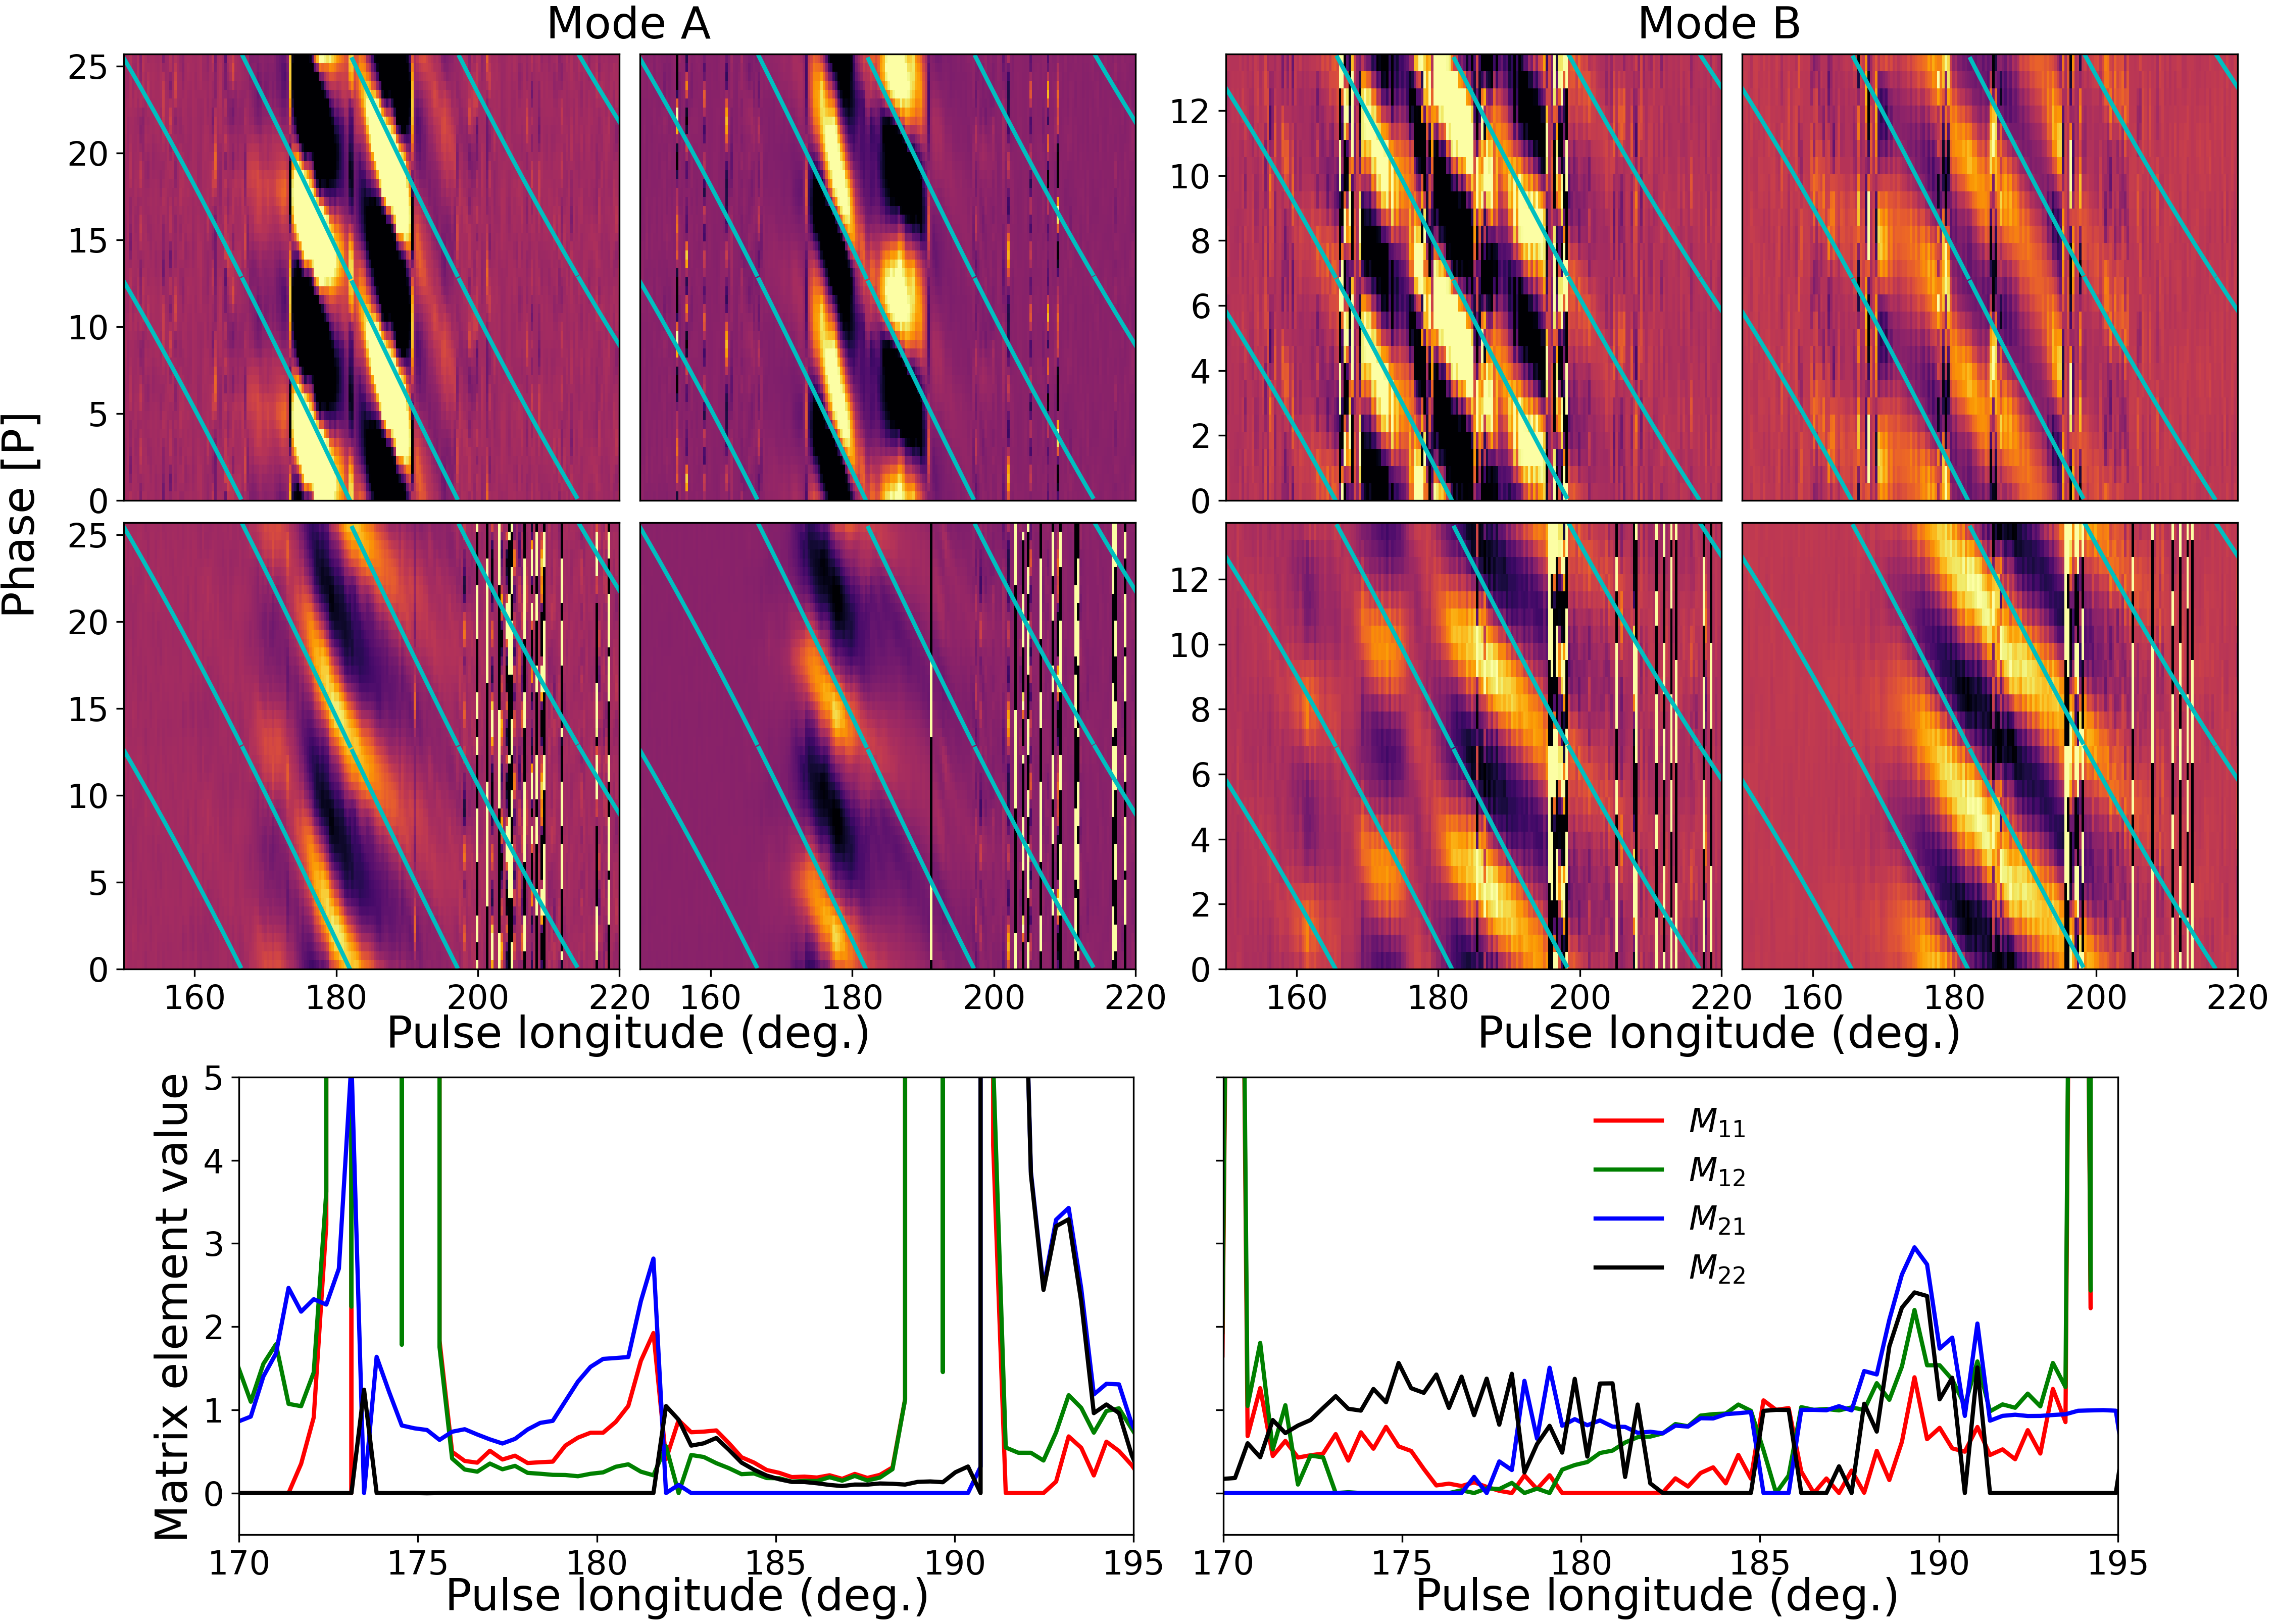
\includegraphics[height=0.66\textwidth]{Figures/B0031/canres_driftbands_2}
            \caption[Results for the canonical model]{The intrinsic and recreated observed driftbands found for the canonical model parameters for each drift mode, along with the associated mixing matrices. Mode A is plotted on the left, and mode B on the right. The upper row of the colour maps shows the intrinsic driftbands, with (arbitrarily labelled) OPM 1 on the left, and OPM 2 on the right. The cyan line shows the contours of constant $\Theta$. The lower colour map shows the recreated observations, which closely match the observed OPMs for each mode as shown in Fig.~\ref{fig: B0031 - observed OPMs}. In all panels the $P_3$ cycle is plotted twice for clarity. The lower line plots show the elements of the fitted mixing matrices as a function of pulse longitude. Where the matrix elements have extreme values as a result of poor fitting, these points have been `skipped' when plotting them, effectively being replaced by interpolated values in order to show the continuous structure. Similarly, the panels showing the driftbands have been clipped in order to show the structure that would otherwise be overwhelmed by the noisy pulse longitudes.}
            \label{fig: B0031 - canonical model driftbands and matrices}
        \end{center}
    \end{figure}
\end{landscape}
\begin{figure}
    \begin{center}
        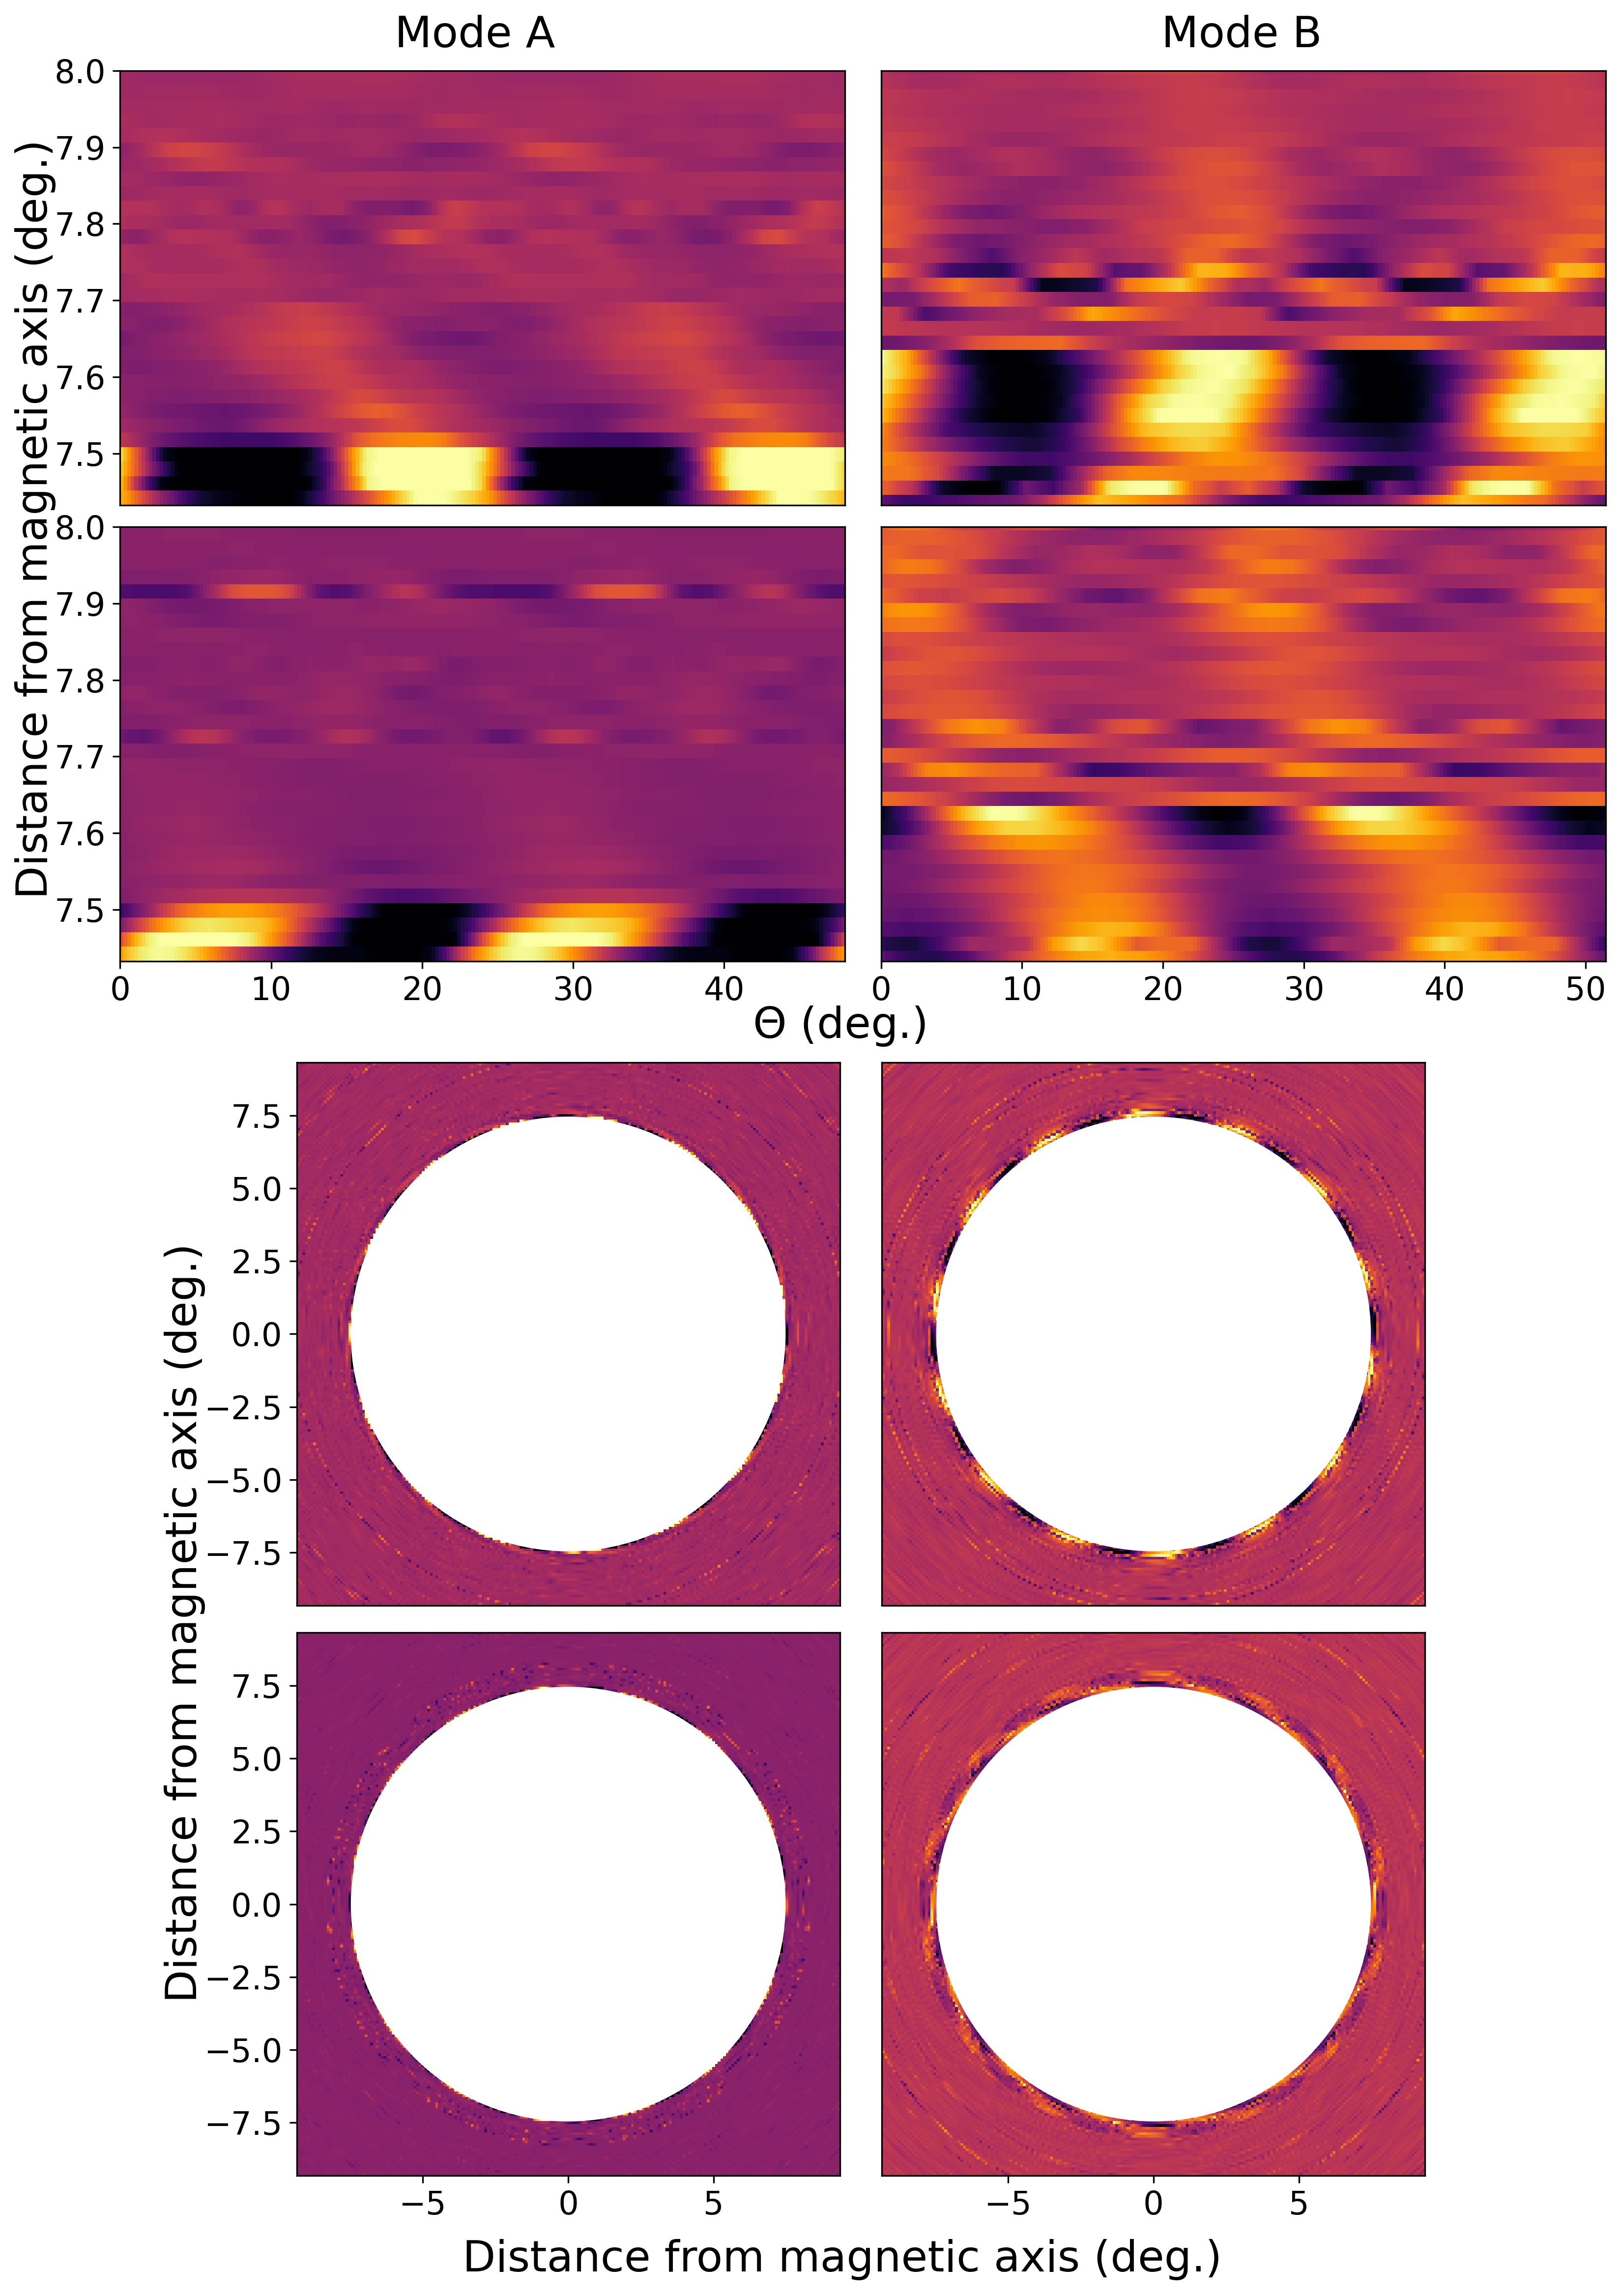
\includegraphics[width=0.8\textwidth]{Figures/B0031/canres_sparks_2}
        \caption[Sub-beams and carousels of the canonical model]{The intrinsic sub-beam structure and carousels of the two OPMs of each drift mode (mode A on the left, and mode B on the right). The upper four panels show a magnified view of the sub-beams in the carousel, plotted in polar coordinates that are treated as Cartesian for ease of illustration ($R$ on the $y$-axis, and $\Theta$ on the $x$-axis). Two sub-beams are shown for clarity. The upper row is OPM 1, and the lower row is OPM 2. The lower four panels show the full polar emission region for each OPM. Again, the upper row is OPM 1 and the lower is OPM 2. The white circle indicates the region where no emission can be observed because of the geometry of the LOS.}
        \label{fig: B0031 - canonical model sparks and carousels}
    \end{center}
\end{figure}

The results for the canonical parameter choice can be seen in Figs.~\ref{fig: B0031 - canonical model driftbands and matrices} and \ref{fig: B0031 - canonical model sparks and carousels}. Figure~\ref{fig: B0031 - canonical model driftbands and matrices} shows the intrinsic driftbands for each drift mode ($I_1$ and $I_2$) found by multiplying the observed OPMs (as seen in Fig.~\ref{fig: B0031 - observed OPMs}) by the inverse of the mixing matrix (Eq.~\eqref{eq: definition of the mixing matrix}). The cyan lines show the contours of constant $\Theta$ determined by the geometry parameters, and calculated using Eq.~\eqref{eq: geometry derivations - P3 phase definition}. For this set of parameters, the gradient of the expected driftband is close to being constant within the on-pulse window spanning $70\degr$. In mode A, OPM 1 has reasonably straight driftbands which closely match the model (cyan curve) whilst the driftbands of OPM 2 have a distinct V-shape -- this is indicative of the sub-beams in the carousel being swept azimuthally. In mode B, both bands trace the contour of constant $\Theta$. For both drift modes there are short intervals of pulse longitude where the driftbands appear discontinuous and noisy: these correspond to those longitudes where the fit was poor, resulting in a poorly constrained mixing matrix. The intrinsic OPM intensities are clipped to optimise the dynamic range of the figure for the regions of interest. The model attempts to find a symmetric intensity distribution in the $P_3$-fold. However, if the geometry parameters are sub-optimal, or if the assumptions made are somewhat oversimplified, there will be a residual asymmetry. To compensate for this, after creating the driftbands they are mirrored about the fiducial plane (along the contour of constant $\Theta$) and averaged. The results shown here are then symmetric. This therefore corresponds to the best-possible symmetric solution. The mixing matrix found is used to see if the observed emission can be reproduced satisfactorily from this symmetric pattern.

The second row of colour plots in Fig.~\ref{fig: B0031 - canonical model driftbands and matrices} show the reproduced observable OPMs using the intrinsic $P_3$-folds which were forced to be symmetric. Applying the mixing matrix to such $P_3$-folds highlights any asymmetries not captured by the model. These errors appear as the bright noise in the final panels, which lie mostly in the regions where little signal is available. The regions with a higher S/N are reproduced well for both modes, and show that the process has largely worked for the canonical model. It can be seen that the `recovered' $P_3$-folds closely match the original observed $P_3$-folds shown in Fig.~\ref{fig: B0031 - observed OPMs}. The chequerboard pattern in the leading half of mode B, OPM 1 has been successfully reproduced, as has the almost rectangular shape of mode A, OPM 2. The faint blob on the leading end of OPM 1 is also recovered well. 

The lower line plots in Fig.~\ref{fig: B0031 - canonical model driftbands and matrices} show the elements of the mixing matrix for drift mode A (left) and mode B (right) that is a result of the fitting at each longitude and after picking out a single solution via the procedure explained in Sec.~\ref{app: matrix maths - posmatrix explanation}. The four matrix elements are plotted in different colours: $M_{11}$ is shown in red, $M_{12}$ in green, $M_{21}$ in blue, and $M_{22}$ in black. For some longitudes, the fitting is poorly constrained because of noise in the data (most notably in the wings of the profile), resulting in erratic evolution of the elements as function of pulse longitude. Although there is some jagged variation in the values of the elements clearly visible in mode B, the matrices are generally smooth as a function of pulse longitude. This result is discussed further in Sec.~\ref{sec: B0031 - discuss - canonical model}.

In Fig.~\ref{fig: B0031 - canonical model sparks and carousels} a close-up view of individual sub-beams for each OPM and drift mode is shown in the top four plots. As in previous figures, mode A is shown in the left-hand panels and mode B in the right, while the upper panels show OPM 1 and the lower panels OPM 2. The sub-beams in these figures have been plotted in Cartesian coordinates, where the $x$-axis is the azimuthal angle in the carousel frame, $\Theta$, and the $y$-axis shows the distance from the magnetic axis, $R$. The minimum $R$-value corresponds to $R=\beta$, so the minimum $R$ probed by the LOS. In each panel of this figure two successive sub-beams are plotted for continuity. The sub-beams of OPM 1 of drift mode A are compact, and located close to the minimum radius but there is evidence of faint, swept-back emission at their outer edge. As predicted from the intrinsic OPM 2 driftband, the sub-beam for mode A is compact but strongly swept forwards. The sub-beams of both mode B OPMs are swept, and in opposite directions, although the sweep of OPM 2 is moderately more severe. Sweeping features could suggest that the canonical geometry is sub-optimal in explaining the observed polarisation, or that the model is somewhat oversimplified. Nevertheless, some sweep could be a real feature caused by refraction, as discussed in Sec.~\ref{sec: B0031 - discuss - atlas - atlas plots evaluation}. In both drift modes OPM 1 appears slightly more compact whereas OPM 2 is more elongated.

The lower four plots in Fig.~\ref{fig: B0031 - canonical model sparks and carousels} show a map of the carousel of sub-beams surrounding the magnetic axis. These illustrate how the carousel would appear to an observer looking down on the pulsar from above, and is the plane defined by the polar coordinates $R$ and $\Theta$ of the cartographic transform. As the structure circulates it is intersected by the observer's line of sight (LOS; not shown) as the star rotates, giving rise to the observed drifting subpulses. The sub-beams are distributed evenly in the azimuthal direction and are identical, a consequence of them being derived from the $P_3$-fold, thereby representing the average sub-beam morphology. There is a gap in the centre of the image for $R<\beta$ where there is no information as the LOS never samples this area. The fact that the sub-beams in both OPMs of both drift modes appear to be very thin in the radial direction whilst elongated in the azimuthal direction may indicate that the LOS only intersects the very edge of the sub-beam. The sub-beams may be larger and more symmetrical structures, with the majority of their emission occurring closer towards the magnetic axis and out of view of the observer.

The goodness-of-fit for the canonical set of parameters was $\chi^2_R = 6.6$ for mode A, and $\chi^2_R = 2.1$ for mode B. Although this indicates the observed emission cannot be fully explained by the model, it has performed very well in reproducing much of the complex behaviour, given the simplifying assumptions made. It also demonstrates the robustness of the model. It does not require fine-tuning to reproduce the data, as most parameters were not optimised to produce this canonical model.






%%%%%%%%%%%%%%%%%%%%%%%%%%%%%%%%%%%%%%%%%%%%%%%%%%%%%%%%%%%%%%%%%%%%%%%%%%%%%%%%%%%%%%%%%%%%%%%%%
%%%%%%%%%%%%%%%%%%%%%%%%%%%%%%%%%%%%%%%%%%%%%%%%%%%%%%%%%%%%%%%%%%%%%%%%%%%%%%%%%%%%%%%%%%%%%%%%%






\subsection{`Atlas' of parameters}
\label{sec: B0031 - results - atlas}

In order to test if the results for the canonical model can be considered robust (i.e. not strongly dependent on parameter choice), we created an atlas of results (as detailed in Sec.~\ref{sec: B0031 - methods - parameter space}) covering different values of each parameter. The full atlas covers a set of 64 different combinations of parameters for each of the two drift modes, i.e. 128 in total. A series of figures for a reduced atlas are shown in Appendix~\ref{app: atlas results} for illustrative purposes, which was pared down to half the solutions explored in total.

The parameters for the atlas are summarised in Tab.~\ref{tab: atlas parameters}. Of the five parameters ($\alpha$, $N$, $n$, $\phi_\mathrm{fid}$, and $m$), four choices for $\alpha$, $N$, and $n$, and three choices for $\phi_\mathrm{fid}$ were specified. In principle the fiducial plane could be placed at the very edge of the observed profile, and this could reproduce the observed asymmetry perfectly. In such a scenario the observed emission forms one side of a much wider cone, with one half being totally attenuated. Such a `trivial' yet somewhat far-fetched solution would not require coupling between the OPMs, hence it is not investigated further. The early, central, and late positions still have a large portion of emission at both sides of $\phi_\mathrm{fid}$, meaning mixing is still required to explain the asymmetry. Initial experiments found that the early and late positions of the fiducial plane resulted in poor results. Therefore, we did not explore these further and focused on the choice of $\phi_\mathrm{fid} = 182\degr$.

As with the canonical model the remaining parameter $m$ was fitted for each choice of the others using a grid search. To keep the analysis simple the two drift modes were approached independently. For mode A, the best driftband gradient was selected from the range spanning $-40$ to $-30$~$P/\text{rad}$ ($-0.70$ to $-0.52$~$P/\degr$), whilst for mode B the range was $-25$ to $-20$~$P/\text{rad}$ ($-0.44$ to $-0.35$~$P/\degr$). As explained in Sec.~\ref{sec: B0031 - methods - parameter space}, the driftband gradient is used as a proxy for $\beta$. The results of the atlas modelling are shown in Appendix~\ref{app: atlas results}, where the figures show the intrinsic driftbands, the recovered observed driftbands and the magnified sub-beams for each atlas entry.

\begin{figure}
    \begin{center}
        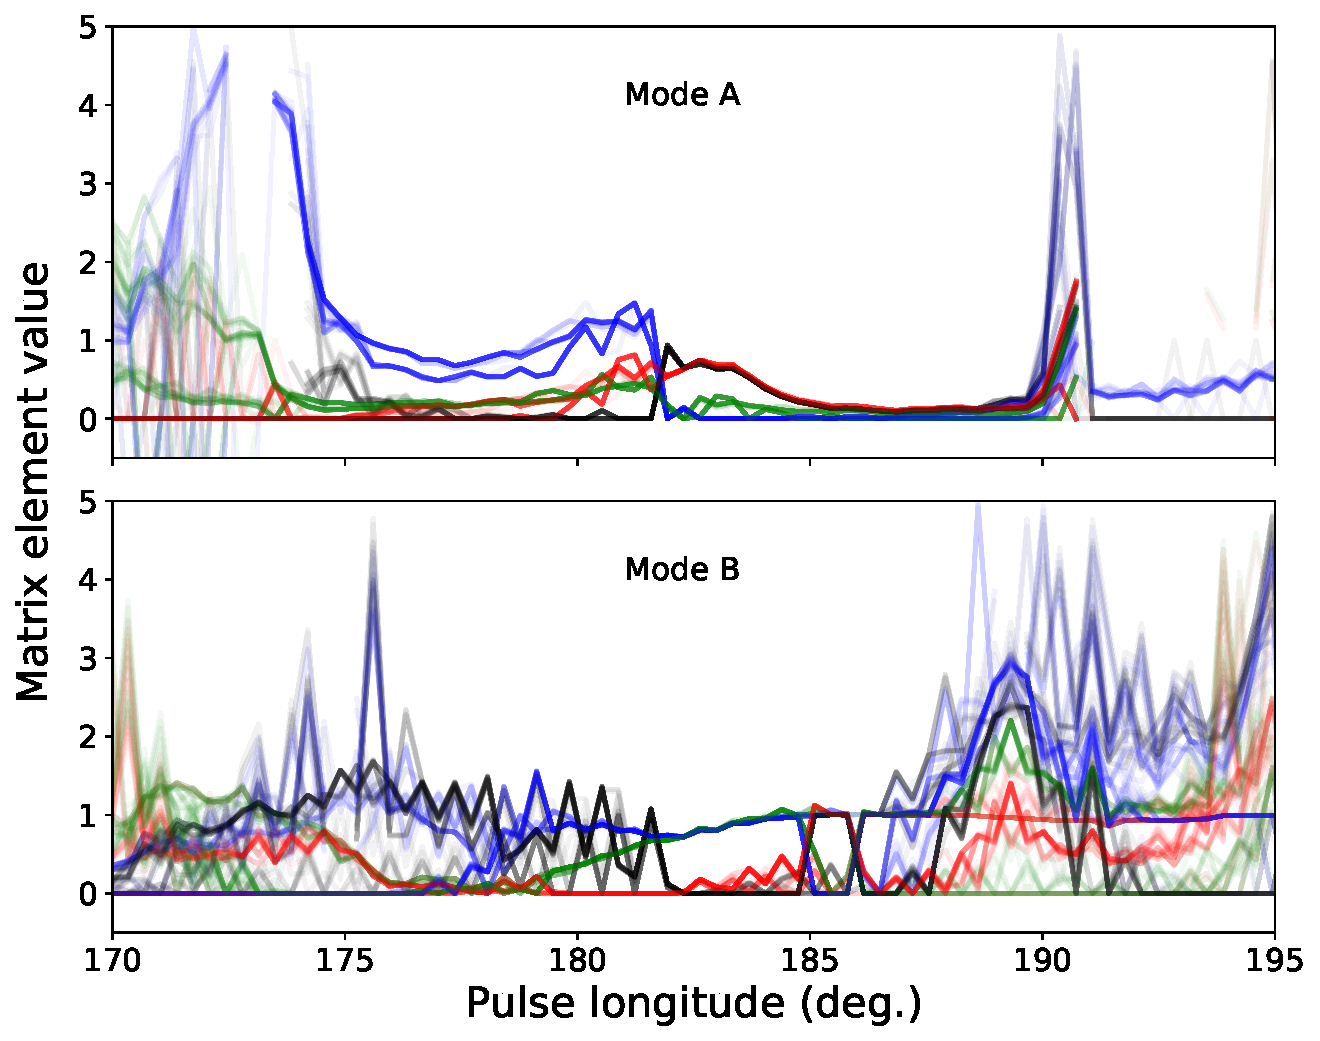
\includegraphics[width=0.8\textwidth]{Figures/B0031/atlas/atlas_matrices}
        \caption[The mixing matrices for the atlas of parameters]{The elements of the mixing matrices produced for the atlas of parameters as a function of pulse longitude. Mode A is shown in the upper panel, and mode B is in the lower panel. The four matrix elements in each are indicated by the coloured lines: $M_{11}$ is red, $M_{12}$ is green, $M_{21}$ is blue, $M_{22}$ is black. The curves appear more opaque where they overlap. As for the matrices shown in Fig.~\ref{fig: B0031 - canonical model driftbands and matrices}, interpolated values are shown for longitudes affected by poor fitting to better show the structure.}
        \label{fig: B0031 - atlas matrices}      
    \end{center}
\end{figure}

In Fig.~\ref{fig: B0031 - atlas matrices} the fitted mixing matrix elements are shown for the 64 solutions for each drift mode to show common features that are independent of the parameter choice. Mode A is shown in the upper panel and mode B in the lower. The range of pulse longitudes shown is limited to $170\degr$ to $195\degr$, as this is corresponds to the region where the results are most stable (i.e. the matrices have generally small values and a clear trend is visible in neighbouring bins).

In both panels the matrix elements appear to be quite robust. In mode A (upper panel) the matrix elements generally vary quite smoothly between pulse longitudes in the on-pulse region, apart from a sharp transition at the fiducial plane. This was expected, given that at this longitude the PA transition is observed to occur in the $P_3$-fold (Fig.~\ref{fig: B0031 - observed P3folds}). At the leading edge of the window, some negative matrix values are still visible -- this is because of floating point precision errors which occur during matrix inversion computation, which especially affects extreme solutions obtained where the observed signal is very weak (and therefore can be neglected). In mode B (lower panel), the mixing matrix in neighbouring longitudes is broadly correlated, and lacks the distinct flip at the fiducial plane seen in mode A. However some variability is visible, especially in the black line (component $M_{22}$) which has a jagged structure such as was observed for the canonical model.

Although the different choices of geometry parameters in the atlas were intended to sample a broad swathe of different potential carousel structures, as for the fitted mixing matrices there are consistent features across the results. To reduce the number of figures in Appendix~\ref{app: atlas results}, results with alias orders $n=5$ and $n=10$ have been omitted, as these higher alias orders are not found to significantly affect the results.

For drift mode A (Figs.~\ref{fig: atlas - MASTER}--\ref{fig: atlas - A_517060014001}), a recurring feature is that at least one of the intrinsic driftbands is V-shaped, meaning that the sub-beams that give rise to this are swept forwards in the azimuthal direction in the carousel frame. This occurs most significantly in OPM 2 (the lower row of panels in each figure), however for some atlas entries the ends of the OPM 1 driftbands (furthest from the fiducial plane) also appear slightly swept forwards. For some geometries there appears to be a small discontinuity in the OPM 1 driftbands on both sides of the fiducial plane, around pulse longitudes $173\degr$ and $191\degr$. Although unclear in the $P_3$-fold, in the magnified sub-beam plot this discontinuity separates two radii of the carousel where the sub-beams appear slightly offset in the azimuthal direction. In some results, for example Fig.~\ref{fig: atlas - A_517005014000}, the discontinuity is present in OPM 2 as well. The sub-beam structure is smooth apart from the discontinuity. This is unlikely to be a `real' structure, in that the boundary appears too sharp to be attributed to nested carousels. It is possible the discontinuity seen in OPM 1 is structure from the more complex driftband shapes of OPM 2 `leaking' into OPM 1. As detailed in Sec.~\ref{sec: B0031 - methods - calculating intrinsic emission - degeneracies}, switching the order of the OPMs is a degeneracy in the solutions. Especially when at least one of the OPMs displays a complex morphology, the algorithm that tries to resolve the degeneracy by forcing smooth structures to be formed might not always succeed.

For mode B the structures seen in the intrinsic driftbands are more diverse. The driftbands as a whole trace the contours of constant $\Theta$ (cyan lines in the $P_3$-folds) without the V-shape that was indicative of strongly swept sub-beams in mode A. Significantly more discontinuities are present in mode B: for example, in Fig.~\ref{fig: atlas - B_517005005000} there is a very sharp jump in the location of the intrinsic OPM 1 driftband at approximately $179\degr$ and $185\degr$, with the portion between these longitudes being offset in $P_3$-fold phase. A similar transition is visible in OPM 2, although this is less abrupt. As shown by the right-hand panels, these transitions are produced by beamlets that are radially extended and vary sharply in azimuth along their length.

Discontinuities of this form are present in nearly all intrinsic driftbands across the atlas for mode B, and as with mode A there appears to be no systematic evolution with the geometry parameters. A recurring feature seen in the magnified sub-beams is that the OPM 2 sub-beams have a backwards sweep ($\Theta$ decreases with increasing $R$) in mode B, whereas OPM 1 of mode A consistently shows a forwards sweep  ($\Theta$ increasing with $R$). From a physical perspective it might be expected that the same sense of sweep is seen in both modes, so this is unexpected -- however, it should be stressed that because each mode was analysed independently they shouldn't be directly compared. This aspect is discussed further in Sec.~\ref{sec: B0031 - discuss - atlas}.

In both drift modes the observed OPMs are recovered well across the atlas, as shown by the middle two plots in each figure in Appendix~\ref{app: atlas results}. For mode A, the change in gradient in the OPM 1 driftband is reproduced, as is the small, faint blob of emission at its leading end. The more compact shape of the OPM 2 driftband is also reproduced well, including its almost rectangular appearance. Similarly, in mode B, the process is clearly successful in reproducing the complex chequerboard pattern at the leading edge of OPM 1 and simultaneously the smooth, continuous bands towards the trailing half (of both OPMs). Compared to the original observed $P_3$-folds (Fig.~\ref{fig: B0031 - observed OPMs}), there appears to be a very small amount of smearing in the $P_3$-fold phase (vertical) direction, the magnitude of which varies stochastically from pulse longitude to pulse longitude. This is most visible in mode A with its higher resolution (due to this mode's greater $P_3$). Some smearing can be expected because the $P_3$-folds of the intrinsic OPMs were forced to be symmetric by averaging data from both sides of the fiducial plane (see Sec~\ref{sec: B0031 - results - literature}). Therefore, any unmodeled features that lead to slight asymmetries will result in broadening. As was the case for the canonical results, there is some bright excess noise in some bins of the $P_3$-folds due to very poor fitting of the mixing matrix. There does not appear to be any systematic variation of where these bad longitudes occur in the atlas results, except that as expected they are more common at locations where the signal is weaker. These results and their implications will be discussed next.







%%%%%%%%%%%%%%%%%%%%%%%%%%%%%%%%%%%%%%%%%%%%%%%%%%%%%%%%%%%%%%%%%%%%%%%%%%%%%%%%%%%%%%%%%%%%%%%%%
%%%%%%%%%%%%%%%%%%%%%%%%%%%%%%%%%%%%%%%%%%%%%%%%%%%%%%%%%%%%%%%%%%%%%%%%%%%%%%%%%%%%%%%%%%%%%%%%%











\section{Discussion}
\label{sec: B0031 - discussion}

The results shown in Sec.~\ref{sec: B0031 - results} and Appendix~\ref{app: atlas results} demonstrate that we have successfully shown that an axially symmetric carousel of sub-beams circulating around the magnetic axis can give rise to the complex, asymmetric $P_3$-folds and polarisation behaviour as observed for PSR~B0031$-$07, if there are two orthogonal polarisation modes which are allowed to mix as they propagate through the magnetosphere. In the following the performance of the canonical model is discussed, and the origin of its parameters is explained. The results of the atlas of geometry parameters are evaluated qualitatively to highlight common features and the goodness-of-fit across the atlas is discussed. Some possible further constraints on the viewing geometry are explained and applied. Finally, the overall results are discussed in the broader context, linking back to the assumptions on which the model was based.


\subsection{The canonical model}
\label{sec: B0031 - discuss - canonical model}

For the `canonical model', which uses parameters for PRS~B0031$-$07 as suggested in the literature, we find a goodness-of-fit (GOF) $\chi^2_R = 6.6$ for drift mode A, and $\chi^2_R = 2.1$ for mode B. This confirms that despite the simplifying assumptions made in the model, it manages to reproduce most details of the complex structures seen in the polarised $P_3$-folds. Mode A has the more complex observed polarisation structures, with reversals in the PA pattern in the leading half of the profile (see Fig.~\ref{fig: B0031 - observed P3folds}, third panels). Despite this, mode B appears to have a much more complex structure in its observed OPMs, in particular the more pronounced chequerboard-like structures in OPM 1 (Fig.~\ref{fig: B0031 - observed OPMs}). The difference in the GOF is likely to be a consequence of the more irregular and curved driftband shapes of the intrinsic OPMs required to fit the observed emission in mode A -- inspection of the $\chi^2$ values (Eq.~\eqref{eq: chi-squared function for asymmetry matrix}) for each pulse longitude bin showed that the fit for mode A was systematically worse than that for mode B, especially closer to the fiducial plane. This potentially means that finer tuning of the geometry parameters is needed or that some assumptions should be relaxed to obtain better fits.

%It is not immediately clear why the GOF is lower for mode B compared to mode A, when from the observed OPMs (Fig.~\ref{fig: B0031 - observed OPMs}) it appears more complex in structure. An onpulse region where the driftbands can clearly be identified is defined for each mode, and the GOF is evaluated over this. Mode A has a smaller on-pulse region by a factor of $\sim$1.4 -- this however should not affect the reduced-$\chi^2$, and does not account for the difference, however a single `bad' fit will carry more weight in this smaller onpulse region. Furthermore, in terms of their shape the mode A driftbands are far more irregular from pulse longitude to pulse longitude, appearing almost rectangular over their short span. This potentially means that finer tuning of the geometry parameters is needed or that some assumptions should be relaxed to obtain better fits.

It should be stressed that during fitting all elements of the mixing matrix were forced to be positive (see Sec.~\ref{sec: B0031 - methods - calculating intrinsic emission} and Appendix~\ref{app: matrix maths - physical constraints}). This physical requirement precludes some possible mathematical solutions that might otherwise fit the data better. So this, alongside other constraints within the model, does not guarantee that good solutions exist for any arbitrary $P_3$-fold. Hence it is highly encouraging that the model produces a good fit. The model was shown to be able to reproduce the data by taking geometrical parameters from the literature, so without any fine-tuning required. As demonstrated by the lower colour plots of Fig.~\ref{fig: B0031 - canonical model driftbands and matrices} which depict the `recovered' observed OPMs arising from a symmetric carousel structure, the observed complexity in the driftbands have been reproduced well. There is slight smearing in the vertical direction which is argued to point towards some asymmetries not being fully reproducible by the model. All main asymmetric features of the observed OPMs shown in Fig.~\ref{fig: B0031 - observed OPMs} have been successfully recovered: these include the small blob on the leading side of mode A, OPM 1, and the chequerboard pattern of OPM 1 of mode B. 

A feature of note is the continuity of the driftbands as seen for the intrinsic OPMs (upper panels in Fig.~\ref{fig: B0031 - canonical model driftbands and matrices}), and the simultaneous continuity of the mixing matrix elements. The continuity of the driftbands was a requirement of the method, achieved by swapping the intensities at a given pulse longitude between the two OPMs if that helps (this is a degeneracy in the model as discussed in Sec.~\ref{sec: B0031 - methods - calculating intrinsic emission - degeneracies}). Swapping of these intensities also necessitates swapping the elements in the columns of the mixing matrix (see Eq.~\eqref{eq: definition of the mixing matrix}). So the elements of the mixing matrix as a function of pulse longitude are not \textit{forced} to be smooth -- nevertheless, this is the case in general. This is what one expects on physical grounds from a magnetosphere with continuous plasma properties and given that the $P_3$-folds are well resolved (without any discontinuities in the observed mode-separated OPMs shown in Fig.~\ref{fig: B0031 - observed OPMs}).

It should be noted that discontinuities in the PA data (for example the OPM transitions visible around the fiducial plane in drift mode A, Fig.~\ref{fig: B0031 - observed P3folds}) do not require a discontinuity in the mode-separated OPMs, nor the mixing matrix. Only a small change in the relative intensities of the OPMs is necessary to produce an OPM transition. However, discontinuities in the observed OPMs do require structure at the corresponding pulse longitude in the mixing matrix. This is further discussed in Sec.~\ref{sec: B0031 - discuss - general discusison}.

% as the figure shows the final matrices are generally smooth. For this dataset with 1024 pulse longitude bins per period, a single longitude bin corresponds to an angle of $0.35\degr$ of stellar rotation. Even taking a low altitude for mixing to occur of 1000~km, this means anisotropies in the magnetosphere would have vary over distances smaller than around 6~km across in order for differences in the mixing matrix to be resolved between longitudes. This is a reasonably large limit, and variations in the magnetosphere can easily occur on smaller scales: for reference, the footprint of the polar cap where the sparks of emission occur has a diameter of $D_\mathrm{PC} \approx 2R\sqrt{R/R_\mathrm{LC}} \approx~300$~m, where $R = 10$~km is the canonical neutron star radius  and $R_\mathrm{LC} = cP/2\pi \simeq  45\times10^{3}$~km  is the light cylinder radius \citep[e.g.][where $c$ is the speed of light]{Sxxx1971}. The observed driftbands are smooth in total intensity which suggests that the magnitude of the variations must intrinsically be small at the altitudes at which mixing may occur.

% Therefore, bin-to-bin variations in the mixing matrix could be expected from both a theoretical (size of the anisotropies) and methodological (forced swapping of neighbouring longitudes) perspective. This could explain the jaggedness of the mode B mixing matrix compared to mode A -- the observed OPMs have a more complex shape (chequerboard pattern), which may be linked to a more turbulent magnetosphere, and hence a greater longitude-to-longitude variation in the mixing matrix would be expected.





\subsubsection{The literature parameter values}
\label{sec: B0031 - discuss - canonical model - literature values}

To create the canonical model we used previously published values of $\alpha$, the number of sub-beams $N$, and the alias order $n$. Here the derivation of these values is discussed, and some of the assumptions that were made.

The value for the magnetic inclination angle came from \citet{SMS+2007}. The authors performed observations of PSR~B0031$-$07 spanning seven different frequency ranges between 150~MHz and 4.85~GHz, using the Giant Metrewave Radio Telescope (GMRT), Westerbork Synthesis Radio Telescope (WSRT), and Effelsberg telescope. They tried three different emission models to model the frequency dependence of the total intensity profile, in order to find a model that reproduced all the features they observed, including the PA curve variations with pulse longitude. Models based on plasma frequency emission and curvature radiation could not reproduce the observations, but an empirical relationship between frequency and emission height that included an extra parameter \citep{Txxx1991} performed well. \citet{SMS+2007} found that RVM models with $\alpha$ between $0.1\degr$ and $6\degr$ were able to reproduce the time-averaged PA curves at different frequencies. We note that because the curvature of the observed PA curve is very low, we find that $\alpha$ and $\beta$ are ill-constrained and highly correlated. However, with a relatively small $\alpha$ \citet{SMS+2007} were able to explain the frequency dependence of the profile width, and the spacing of the subpulses ($P_2$), independent of the polarisation information. Therefore $\alpha = 5\degr$ was considered an appropriate and justifiable value for the canonical model. More detail on the argument that PSR~B0031$-$07 might be a more aligned rotator based on its profile width can be found in Sec.~\ref{sec: B0031 - discuss - atlas - beta constraint}.


% \todo{The viewing geometry was constrained from an initial fit of the RVM, and they found that a range of values between $0.1\degr$ and $6\degr$ was able to reproduce the PA curves at different frequencies.

% \citet{SMS+2007} focused on RVM fitting of data averaged over many pulses, so they would not have observed the intensity modulated OPM changes observed by \citet{IWJ+2020}. They recognised the presence of OPMs and took these into account in their fitting process. Fitting the RVM was also attempted in this work using the single pulse data to better resolve the OPM transitions, but it did not lead to useful constraints since the curvature of the observed PA curve is very low, and thus the $\alpha$ and $\beta$ found using this method are tenuous. Nevertheless, a low $\alpha$ was also found by \citet{SMS+2007} to be able to explain the frequency dependence of the profile width, and the spacing of the sub-pulses ($P_2$), independent of the polarisation information. Therefore $\alpha = 5\degr$ was considered an appropriate and justifiable start point.}

% Forward reference to \ref{sec: B0031 - discuss - atlas - beta constraint}

The values used for the number of sub-beams in the carousel of each mode and their alias orders are those published by \citet{MBW+2019}. The authors take a different approach to \citet{SMS+2007} when examining the drifting subpulses of this pulsar, focusing instead on the periodicities in the pulse stack. They argue that a constant carousel circulation period $P_4$ for all three drift modes is more consistent with the original model of \citet{RSxx1975}, as the speed is determined by the magnetic and electric fields near the surface of the star where the sparks that feed the beamlets occur. These fields cannot easily change their magnitude and/or directions on the timescales at which mode changes can occur (less than one pulse period). Under this assumption, to explain the difference in $P_3$ for each drift mode ($P_3^{(A)} \approx 13P_1$, $P_3^{(B)} \approx 7P_1$, $P_3^{(C)} \approx 5P_1$), \citet{MBW+2019} instead investigate whether a change in the number of beamlets can be responsible. The requirement that $\Delta N$ be an integer immediately means that the alias order cannot be zero for all three drift modes. They argue that if the alias order is the same for all three, then $1/P_3$ is an arithmetic sequence, with the n\textsuperscript{th} term corresponding to a carousel with $N$ sub-beams. If $N_A$, $N_B$, and $N_C$ are in turn themselves part of a sequence, then the values of $P_3$ will be harmonically related (as suggested by \citealt{WFxx1981}), and this can be shown to be the case for PSR~B0031$-$07.
In the special case that the number of beamlets changes by only one between the different drift modes, \citet{MBW+2019} showed that $N_A = 15$, $N_B = 14$, and $N_C = 13$ is a self-consistent solution. This suggests that $n=1$, giving $P_4 \eqsim 16.4 P_1$. Although the \citet{RSxx1975} model predicts a smaller $P_4 \approx 4$, they argue that this solution is much closer to the theoretical value than an unaliased solution. The \citet{RSxx1975} model is well known to predict relatively short circulation periods, and screening of the electric field could be responsible for the difference (e.g. \citet{Sxxx2013} -- it should be noted that this may conflict with the prior assumption of \citet{MBW+2019} that $P_4$ be the same for all drift modes, as the plasma distribution (and hence screening) could differ between modes).

There is a conflict between \citet{SMS+2007} and \citet{MBW+2019}. \citet{SMS+2007} assume that the drifting subpulses are not aliased, and derive the rotation time and number of carousel sub-beams directly from the observed $P_3$ values. They fix the number of sub-beams at $N=9$ for each drift mode, meaning that $P_4$ must change. On the other hand, \citet{MBW+2019} make no comment on $\alpha$ or $\beta$ but do allow aliasing to take place. Therefore, the values used for the canonical model are not fully compatible with all the discussed models. However, since the \citet{MBW+2019} results do not rely on a particular $\alpha$ or $\beta$, the parameters of the canonical model are fully consistent with the \citet{MBW+2019} model. Moreover, there are significant uncertainties associated with each of the parameters used -- this further suggests that the model does not require fine tuning in order to reproduce the observed polarised drifting subpulse patterns.

%%%%%%%%%%%%%%%%%%%%%%%%%%%%%%%%%%%%%%%%%%%%%%%%%%%%%%%%%%%%%%%%%%%%%%%%%%%%%%%%%%%%%%%%%%%%%%%%%
%%%%%%%%%%%%%%%%%%%%%%%%%%%%%%%%%%%%%%%%%%%%%%%%%%%%%%%%%%%%%%%%%%%%%%%%%%%%%%%%%%%%%%%%%%%%%%%%%




\subsection{Atlas of geometry parameters}
\label{sec: B0031 - discuss - atlas}

The atlas of parameters provides a robust examination of the effect of how the choice of the geometry parameters affects the results, and serves to reinforce the findings of the canonical model.

\subsubsection{Goodness-of-fit in the atlas}
\label{sec: B0031 - discuss - atlas - chi2}

As explained in Sec.~\ref{sec: B0031 - results - atlas}, there does not appear to be any systematic variation of the appearance of the results across the entries of the atlas: this is also the case for the goodness-of-fit for each entry. The distribution of reduced-$\chi^2$ values is shown in Fig.~\ref{fig: B0031 - atlas chi2}, where the results for mode A are shown in red and mode B is shown in blue. For mode A, the reduced-$\chi^2$ values are clustered between $4.5$ and $6$, distinctly smaller than the value of $6.6$ obtained for the canonical model. This is not unexpected, since for the canonical model the driftband gradient was forced by a choice of $\beta$ (chosen by fitting the driftband gradient of mode B), whereas in the atlas it is optimised for each entry. The values for mode B are all grouped around the canonical model value of $2.1$, indicating that the specific parameter choice for the canonical model does not perform significantly better than any other. 
\begin{figure}
    \begin{center}
        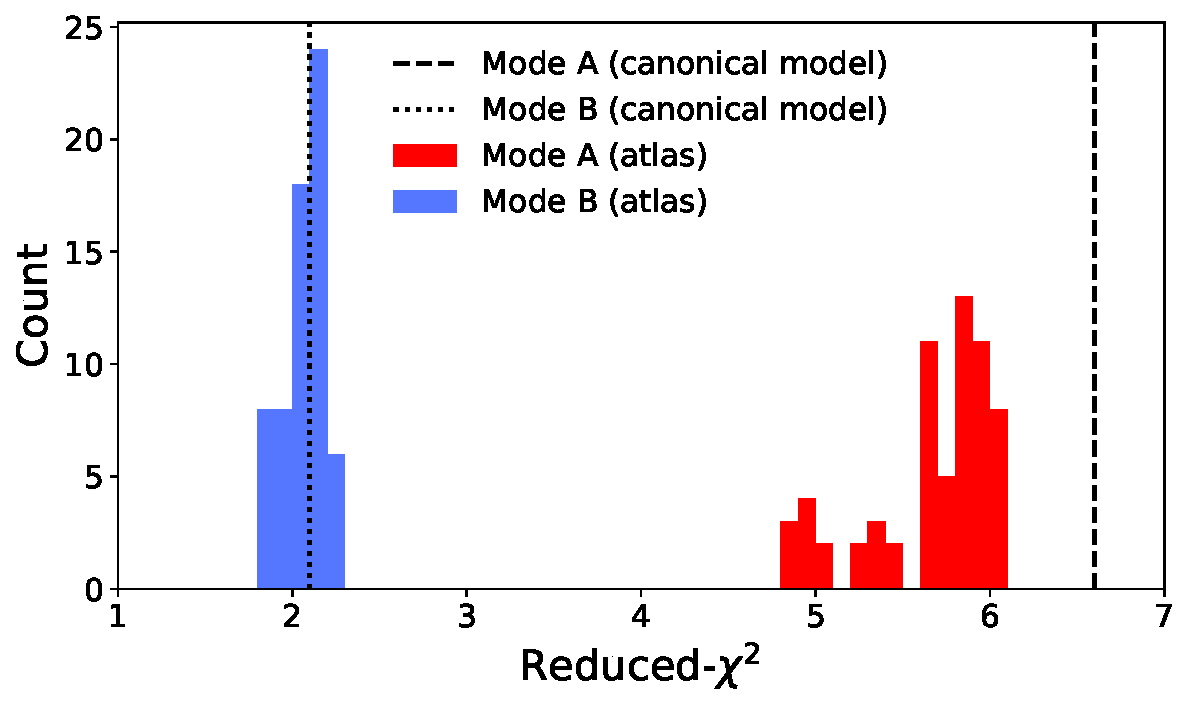
\includegraphics[width=0.75\textwidth]{Figures/B0031/atlas_chi2_hist}
        \caption[Distribution of the goodness-of-fit of the atlas results]{A pair of histograms showing the distribution of reduced-$\chi^2$ values across the 128 atlas entries for drift mode A (red) and mode B (blue). The values for the canonical model parameters for each mode are shown by the dashed and dotted lines respectively.}
        \label{fig: B0031 - atlas chi2}
    \end{center}
\end{figure}
In both modes the reduced-$\chi^2$ is consistently greater than one, without a discernable systematic dependence on the parameter choice. %This was expected to some degree by the degeneracies in the geometry highlighted in Sec.~\ref{sec: B0031 - methods - calculating intrinsic emission} which mean that a reasonable solution can always be found if the driftband gradient is allowed to vary. The clustering of the distributions around the goodness-of-fit found for the canonical model shows that this result is robust.

These results show that the model is robust in the sense that it is insensitive to the geometry parameters that must be assumed. Although the robustness of the mixing model leads to the qualitative conclusion that it can successfully explain the observed asymmetries with an underlying axisymmetric carousel, it also highlights that it is unsuccessful in obtaining meaningful constraints on the required geometry parameters. This may not be surprising given that the duty cycle of PSR~B0031$-$07 over which emission is observable is somewhat limited. This leads to degeneracies between parameters, similar to the process of fitting the RVM to polarisation data (see for example Sec.~\ref{sec: J1926 - analysis - polarisation}). Although more sensitive observations could potentially help for this pulsar, the benefit will be limited.


% This result serves to show that applying the mixing model only leads to qualitative solutions about whether or not a carousel is the source of emission, and it cannot be used to actually quantify the parameters that describe it with precision. Attempting to minimise the reduced-$\chi^2$ of the fit to do so would be fruitless because of the noise in the data which means that underlying systematics cannot be identified -- using data with a higher signal-to-noise ration may lead to a way to constrain the geometry, although the degeneracy of the parameters still remains. The number of assumptions incorporated into our model, from the nature of the carousel emission to the mode separation methods in particular, meant that it was only ever expected to work to first order. Despite this, we have shown that the mixing of the intrinsic modes required to reproduce the asymmetric observations is robust, and independent of the specific geometry of PSR~B0031$-$07

\subsubsection{The fitted mixing matrices}
\label{sec: B0031 - discuss - atlas - mixing matrix}

Figure~\ref{fig: B0031 - atlas matrices} demonstrates that we find a consistent evolution of the mixing matrix elements with pulse longitude over the high S/N on-pulse region, regardless of the choice of geometry parameters for a given drift mode. Although the atlas results suggest that the geometrical parameters related to the carousel structure cannot be constrained by the mode, the required mixing as quantified by the asymmetry matrix \textit{is} constrained. Here it should be noted that the mixing of the OPMs should take place high in the magnetosphere, far from the polar cap where the carousel structure is produced by `sparks' close to the surface of the pulsar (Sec.~\ref{sec: B0031 - introduction}).

While the matrix is similar for all atlas entries of a given drift mode, there is a clear difference in its structure \textit{between} the two modes as shown by the difference between the two panels of Fig.~\ref{fig: B0031 - atlas matrices}. This was not unexpected -- if the magnetosphere must reconfigure to give rise to the significantly different carousel and polarisation properties during mode switching, there is no reason why the magnetospheric mixing and attenuation during propagation would not be affected. As such, this means that mode switching should be considered to be a \textit{global} magnetospheric phenomenon rather than something that only affects the polar cap area. This is not a new idea: for example, nulling (see Chapter~\ref{chapt: J1926} for instance) is thought to be an extreme form of mode change \citep[e.g.][]{Bxxx1992,WMJx2007} caused by the global reconfiguration of magnetospheric currents \citep{KLO+2006,Txxx2010b}. 

The mode changes in PSR~B1957+20 that affect multiple components in both the main and interpulse profiles \citep{MKMP2018} also provide evidence for large-scale magnetospheric changes. \citet{WWJx2012} noted that PSR~B1055$-$52, which is a nearly orthogonal rotator, exhibits phase-locked modulation in the emission from both its magnetic poles. A comparable behaviour was observed in PSR~B1702$-$19, which has periodic modulation with $P_3 \sim 11P_1$ in both its main pulse and interpulse profiles, with a phase lag of approximately half a stellar rotation \citep{WWSx2007}. A third example of global magnetospheric changes are found for another interpulse pulsar, PSR~B1822$-$09 \citep{BMRx2010}. This object displays mode-switching behaviour, with distinct `bright' (B) and `quiescent' (Q) states \citep{FWMx1981}. In the B-mode, the main pulse gains an additional profile component whilst the interpulse emission vanishes -- the intensities of the radiation produced by the two poles are anti-correlated \citep{FWxx1982, GJKx1994}. This persists in the Q-mode, to a lesser extent \citep[Fig. 11]{BMRx2010}. Overall, these objects provide strong evidence that emission is influenced by global magnetospheric behaviours, which might well apply to PSR~B0031$-$07 as well.


\subsubsection{Evaluation of the atlas plots}
\label{sec: B0031 - discuss - atlas - atlas plots evaluation}

To reiterate the point raised in Sec.~\ref{sec: B0031 - methods - calculating intrinsic emission - degeneracies}, the intrinsic OPMs shown ($P_3$-folds and carousels such as in Fig.~\ref{fig: B0031 - canonical model sparks and carousels}) are not unique solutions, nor are the mixing matrices. The intrinsic OPMs shown in Appendix~\ref{app: atlas results} may still be a linear combination of X- and O-mode emission, as the mixing matrices shown in Fig.~\ref{fig: B0031 - atlas matrices} are only one possible solution to the degeneracy, as explained in Sec.~\ref{sec: B0031 - methods - calculating intrinsic emission - degeneracies}. That said, the atlas of results can provide some insight into the required carousel structure when the entries share common features. 

In the atlas, we found that for mode A one intrinsic OPM (usually OPM 2) exhibited V-shaped driftbands whereas the other largely traced the contours of constant $\Theta$. This is a consequence of the beamlets being swept azimuthally in the carousel, and the non-swept beamlets are more compact. This could be related to refraction effects, as introduced in Sec.~\ref{sec: B0031 - introduction}. \citet{BAxx1986} associated the two OPMs with the O- and X-mode propagation of radiation in a strongly magnetised, ultra-relativistic plasma. The X-mode experiences no refraction whereas the O-mode does, and therefore is slightly delayed in pulse longitude. The swept-out sub-beams of OPM 2 could be a signature of refraction that distorts initially compact beamlets, such as seen in OPM 1. We assigned the labels OPM 1 and OPM 2 arbitrarily so they are not necessarily associated with a specific plasma mode; nevertheless, the consistency of the sub-beam shape across the mode A atlas means that the patterns labelled OPM 1 and 2 may be dominated by X- and O-mode emission respectively.

The mode B results show much more variability across the atlas, with much more complex driftband shapes. As explained in Sec.~\ref{sec: B0031 - results - atlas} there are some entries which show a sweep in the beamlets for one or both of the OPMs, but nowhere near as consistently as in mode A. The more common feature is a discontinuity in the driftband which originates from two concentric rings of beamlets, offset azimuthally in the carousel frame. The amount of offset varies, as does the sharpness of the transition. These discontinuities are likely caused by confusion of the smoothing algorithm rather than any real feature in the intrinsic driftbands, which are otherwise smooth. As explained in Sec.~\ref{sec: B0031 - methods - calculating intrinsic emission - degeneracies}, one of the steps taken in producing the intrinsic driftbands is to swap intensities between the two OPMs in order to make the driftbands as continuous as possible. This process begins at the fiducial plane and moves outward, and two sets of longitudes in the leading and trailing halves are compared simultaneously with the neighbouring (inner) longitudes. Initially (close to the fiducial plane) the driftbands of mode B are very smooth and have a high S/N so this process is reliable and will always lead to smooth results. However, around $177\degr$ pulse longitude OPM 2 becomes significantly weaker (see Fig.~\ref{fig: B0031 - observed OPMs}), corresponding to the location of the discontinuity in the intrinsic OPM. The smoothing algorithm was likely confused by the noisy pulse longitude bins in the intrinsic OPMs caused by poor fitting to the weak signal in the observed OPM 2, coupled with the transition to the chequerboard-like pattern in OPM 1.

Clearly the observed mode B is much more complex than mode A in terms of the separated observed OPMs (Fig.~\ref{fig: B0031 - observed OPMs}), but arguably also in total intensity (Fig.~\ref{fig: B0031 - observed P3folds}, top panels). The question is, from where should the complexity originate? The carousel of sparks should arguably be relatively simple in structure if it is to be maintained during circulation in the polar cap. That would favour beamlets that are compact as seen for example in PSR~B0809+74 \citep{RRL+2006}, but note also that one OPM on this carousel (their Fig.~10) has swept sub-beams as we found in mode A of PSR~B0031$-$07. Our method of determining the mixing matrix from the fitted asymmetry matrix (Appendix~\ref{app: matrix maths - posmatrix explanation}) attempts to force as much of the complexity into the mixing matrix (i.e. magnetospheric processes) and have the carousel be as simple as possible. The discontinuities in the fitted intrinsic driftbands of mode B suggests that some complexity still remains in the intensity rather than the mixing matrix. Here it should be stressed that the intrinsic beam patterns derived may have been affected by refractive processes in the magnetosphere (see Sec.~\ref{sec: B0031 - methods - magnetospheric distortions}), which will add complexity on top of the pattern of sub-beams produced in the polar cap.


\subsubsection{Further constraints on the geometry}
\label{sec: B0031 - discuss - atlas - beta constraint}

A further constraint on the results to be considered comes from the values of the impact parameter $\beta$ in the atlas. In order for emission to be observed, the observer's line of sight must intersect the emission cone surrounding the magnetic axis. The relationship between the observed profile width $W$ (assuming the emission fills the open-field-line region), the geometry of the LOS as quantified by $\alpha$ and $\beta$, and the half opening angle of the emission cone $\rho$ is
\begin{equation}
    \label{eq: B0031 - allowed geometry}
    \cos\rho = \cos\alpha\cos(\alpha+\beta)+\sin\alpha\sin(\alpha+\beta)\cos\bigg(\frac{W}{2}\bigg),
\end{equation}
as derived by \citet{GGRx1984}, and see also Appendix~\ref{app: geometry derivations}. For the LOS to intersect the cone, $\rho \geq |\beta|$. In our method $\beta$ was not an input into the model directly, but rather was derived from the best-fitting driftband gradient in combination with the other parameters (see Sec.~\ref{sec: B0031 - methods - parameter space}). Figure~\ref{fig: B0031 - atlas alpha vs beta} shows the derived values for the LOS colatitude $\alpha + \beta$ corresponding to the different values of $\alpha$ -- results for mode A are shown in red, and for mode B they are blue.
\begin{figure}
    \begin{center}
        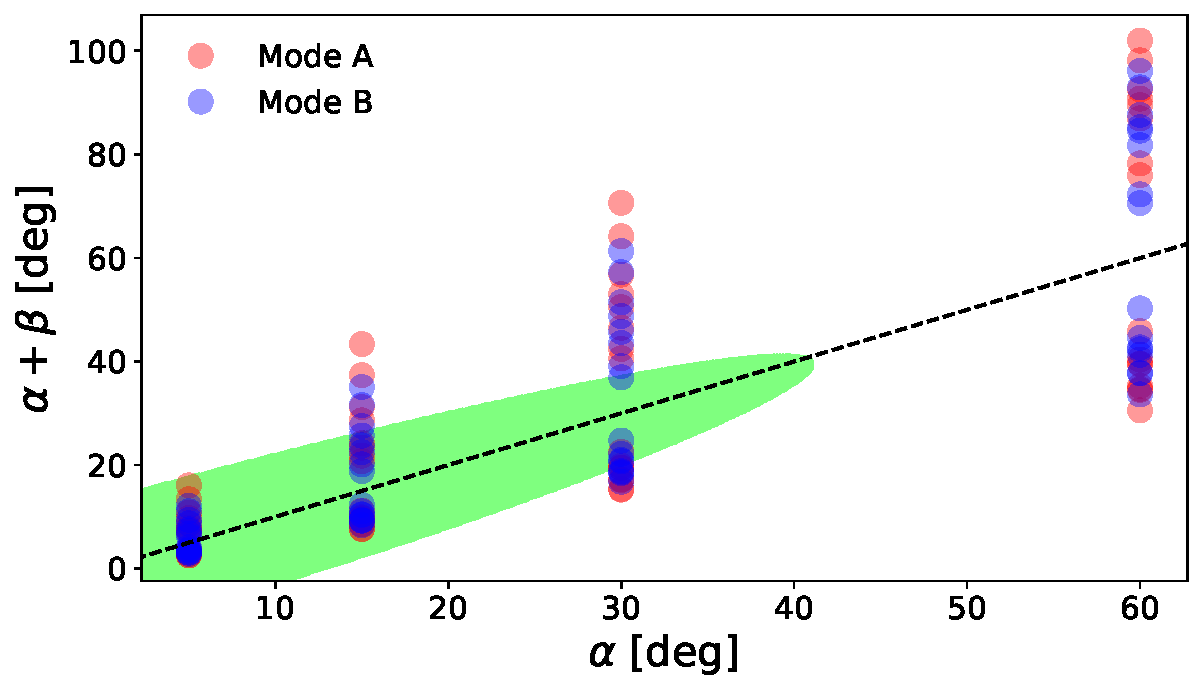
\includegraphics[width=0.75\textwidth]{Figures/B0031/alpha_zeta_distribution}
        \caption[Distribution of $\alpha$ and $\beta$ in the atlas of results]{The colatitude of the LOS $\alpha + \beta$ plotted against the magnetic inclination angle $\alpha$ for the atlas of results. Mode A is shown in red, and mode B is shown in blue. Mode A permits slightly larger values of $|\beta|$ than mode B due to larger driftband gradient, $m$. The dashed black line indicates $\beta = 0$. The green region indicates which values of $\alpha$ and $\beta$ satisfy Eq.~\eqref{eq: B0031 - allowed geometry} for a profile width of $W = 40\degr$ and emission cone half opening angle $\rho = 13\degr$.}
        \label{fig: B0031 - atlas alpha vs beta}     
    \end{center}
\end{figure}
The sign of $\beta$ depends on the alias order, as seen in Eq.~\eqref{eq: driftband gradient}. This is because the apparent drift direction depends on the alias order, and it also depends on whether the carousel is viewed by an inner or outer line of sight. The observed driftbands have a negative gradient, and this is predicted if $\beta < 0$ for even alias orders, and $\beta > 0$ for odd alias orders as shown in Appendix~\ref{app: geometry derivations}. %A hard geometry requirement is that $0\degr \leq \alpha + \beta < 180\degr$ and all values in Fig.~\ref{fig: B0031 - atlas alpha vs beta} satisfy this. If any atlas entry had broken this constraint this would have provided a way to rule out that choice of the other geometry parameters ($N$, $n$, and $\alpha$). 

In both modes in the atlas, $\beta$ is in general permitted to be quite large, especially for large values of $\alpha$: this would require very large emission cones. The opening angle of the emission cone is governed by the tangents to the last open field lines at the emission height, so a large cone in turn requires exceptionally large altitudes. Given PSR~B0031$-$07 is a `normal' pulsar in terms of its spin properties, this seems unlikely \citep[e.g][]{GLxx1998,  WJxx2008, JKxx2019}. 
Assuming an upper bound on the emission height $h_\mathrm{em}$ of 1000~km \citep[e.g.][]{KJxx2007}, the opening angle of the emission cone is given by 
\begin{equation}
    \label{eq: B0031 - cone angle}
    \rho = \sqrt{\frac{9\pi h_\mathrm{em}}{2cP}}
\end{equation}
in the small angle limit \citep[e.g. $h_\mathrm{em} \ll R_\mathrm{LC}$,][]{Rxxx1990}. This gives $\rho \approx 13\degr$. The profile width of PSR~B0031$-$07 $W \approx 40\degr$. Substituting these values into Eq.~\eqref{eq: B0031 - allowed geometry} provides a way to constrain values of $\alpha$ and $\beta$ which satisfy the relation. These `allowed geometries' are shown as the green region in Fig.~\ref{fig: B0031 - atlas alpha vs beta}, and indicate that $\alpha \lesssim 40\degr$. This provides an argument that lower values of $\alpha$ are desirable, in agreement with the modelling of \citet{SMS+2007} which was based on the observed profile width and frequency dependence of $P_2$. In this it should be noted that we only considered a relatively small sample of values for $N$ and $n$ in our atlas, which also contribute to $\beta$ for a given $\alpha$ and measured driftband gradient $m$ (Eq.~\eqref{eq: driftband gradient}). However, the sample covers a wide range of possible parameter space. The dependence of $|\beta|$ on these two parameters is only a small, positive correlation, so does not greatly affect our overall conclusions.





%%%%%%%%%%%%%%%%%%%%%%%%%%%%%%%%%%%%%%%%%%%%%%%%%%%%%%%%%%%%%%%%%%%%%%%%%%%%%%%%%%%%%%%%%%%%%%%%%
%%%%%%%%%%%%%%%%%%%%%%%%%%%%%%%%%%%%%%%%%%%%%%%%%%%%%%%%%%%%%%%%%%%%%%%%%%%%%%%%%%%%%%%%%%%%%%%%%








\subsection{General discussion}
\label{sec: B0031 - discuss - general discusison}

A key assumption in this work is that coupling of the OPMs can occur in the pulsar, at altitudes higher than those at which refraction is the dominant magnetospheric effect on polarisation. This has been suggested in the literature, but is at some level a simplification as refraction and mode coupling are closely related phenomena. For example, \citet{Pxxx2001} argues that refraction is significant only at distances of the order of the emission altitude since the plasma number density rapidly decreases with altitude ($\rho \propto r^{-3}$; e.g. \citealt{RSxx1975}).
At the altitudes at which emission is produced, the two modes do not interact with each other and their polarisation evolution can be described in terms of geometrical optics -- the plasma is sufficiently dense that refraction is a significant effect. At some point during their propagation, the light rays will travel quasi-longitudinally with the local magnetic field lines, at which point geometrical optics fails. In this region of conversion \citet{Pxxx2001} argues that energy can be transferred from the subluminous O- to the superluminous X-mode. Eventually, the rays deviate from the magnetic field once more; mode coupling no longer takes place, and geometrical optics is once again valid. However, the plasma density has fallen by this point such that refraction is no longer significant. The waves propagate independently, although they may acquire some circular polarisation and the PA may rotate slightly until they reach the polarisation limiting region \citep{PLxx2000, Pxxx2001}.


An important step in applying our model was separating the observed polarised emission into two independent OPMs, broadly following the method of \citet{MSxx2000}. The mode separation was built on assumptions which will affect the results if inaccurate. The assumptions made were 1) that the two OPMs are perfectly orthogonal, and 100~per~cent linearly polarised, and 2) that the OPMs combine by incoherent mode addition. As explained in Sec.~\ref{sec: B0031 - methods - mode separation}, we neglected the circularly polarised emission as it is considerably weaker than the linearly polarised emission, so contributes very little to the overall intensity of both Stokes $I$ and the two orthogonal modes. However, the presence of circular polarisation gives rise to strange behaviour in the $P_3$-folds, as noted by \citet{IWJ+2020}. At the PA transition, where the dominant OPM switches, the ellipticity angle is at its maximum, where the expected signature of truly orthogonal emission is that it should be zero. This can possibly be explained if the two OPMs are not perfectly orthogonal, such that the ellipticity angle of one OPM is slightly larger than the other. Then, at a transition, as one OPM decreases in intensity and the other increases, the resultant vector on the Poincar\'e sphere would sweep round in azimuth (PA), but also pass through one of the poles (associated with pure Stokes $V$) in the process. Non-orthogonal polarisation modes may therefore need to be considered in order to more accurately mode-separate the data, but the methods would be much more complex as this would require knowledge about the ellipticity angles of each mode, as well as whether their offset remains constant at all times. Given the small degree of circular polarisation in PSR~B0031$-$07, this will be of little consequence.


One can also consider what effect coherent mode addition may have. In that case it is in principle possible to produce any orientation of a vector in the Poincar\'e sphere by summing the two contributing modes with a suitable intensity ratio and phase offset \citep[e.g.][]{Dxxx2017}. Coherent processes are thought to take place in pulsar magnetospheres; for example it is coherent radio emission from bunches of charged particles which leads to the bright polarised emission in the first place \citep{RSxx1975}. While all radiation is produced coherently on a microscopic scale, radiation originating from macroscopically separated locations in the magnetosphere do not necessarily add coherently, as this depends on the coherence length of the radiation. As for non-orthogonal polarisation modes, attempting to explain the observations as coherent mode addition requires more assumptions on the magnitudes, orientations, and phases of the constituent waves, thereby making the model less constraining. We know that incoherent mode addition must play a role given the significant degree of depolarisation observed for PSR~B0031$-$07. The approach of taking incoherent mode addition as the basis for modelling can therefore be viewed as a first-order approximation. 

Although we have demonstrated that the OPM mixing model could explain complicated pulsars such as PSR~B0031$-$07, the resulting degeneracies in the solutions make it hard to reach any firm conclusions about the behaviour of the pulsar magnetosphere. However, the relative amplitudes of the mixing matrix elements can give some information on the origin of the structures visible in the observed OPMs. For example, consider OPM 2 of drift mode A (lower left panel of Fig.~\ref{fig: B0031 - observed OPMs}): at approximately $182\degr$ there is a slight `kink' in the observed driftband such that there appears to be an offset in phase. In the fitted mixing matrix for both the canonical model (Fig.~\ref{fig: B0031 - canonical model driftbands and matrices}; lower left panel) and the atlas (Fig.~\ref{fig: B0031 - atlas matrices}), element $M_{21}$ (blue line) is strong in the leading half while $M_{22}$ (black line) is close to zero, and vice versa in the trailing half. This shows that the kink in the observed OPM is due to a sudden swap between emission from intrinsic OPM 1 to intrinsic OPM 2. In the framework of \citet{Pxxx2000} this may indicate a transition between a region where mode conversion is a strong effect to one where it is not, caused by the geometry of the underlying magnetic field and/or plasma distribution at the observed pulse longitude. 

% \todo{For example, when pairs of elements switch this tells use where the dominant mode changes. A solution for the mixing matrix which is the same for two drift modes could exist, but not for PSR~B0031$-$07. This can be seen from the observed OPM $P_3$-folds as shown in Fig.~\ref{fig: B0031 - observed OPMs}. Looking at OPM 1 in this Figure (upper $P_3$-fold panels), there is a region between pulse longitudes $170\degr$ to $180\degr$ where mode A has a continuous driftband but mode B is in a transition state. This cannot occur if the mixing matrix were the same in both modes, and serves to illustrate that the state of the magnetosphere must change between modes, in a way that is not just limited to the emission region.}

The chequerboard pattern in the observed leading half of mode B led to the expectation that mode switching is occurring often across this region, and this is borne out in the mixing matrix shown in Fig.~\ref{fig: B0031 - canonical model driftbands and matrices}. On the other hand, the mixing matrix for mode A is much smoother and transitions happen less frequently. The evidence of more complex mixing behaviour for mode B may suggest that the magnetosphere is becoming less homogeneous in this mode. It is not clear whether a change in the carousel morphology triggers the more variable magnetosphere, or vice versa, or indeed if the two are independent but symptoms of some larger underlying change. If extensions to this model are to be explored, then some model of how the mixing depends on the state of the magnetospheric plasma is required. This can then lead to predictions of the mixing matrix from a given carousel state which could then be tested against observations.





%%%%%%%%%%%%%%%%%%%%%%%%%%%%%%%%%%%%%%%%%%%%%%%%%%%%%%%%%%%%%%%%%%%%%%%%%%%%%%%%%%%%%%%%%%%%%%%%%
%%%%%%%%%%%%%%%%%%%%%%%%%%%%%%%%%%%%%%%%%%%%%%%%%%%%%%%%%%%%%%%%%%%%%%%%%%%%%%%%%%%%%%%%%%%%%%%%%








\section{Conclusions}
\label{sec: B0031 - conclusion}


Overall, it has been successfully established that asymmetric driftband patterns in both total intensity and polarisation can be caused by the pulsar magnetosphere distorting the emission from (circular) axisymmetric carousel-like structures. Here the asymmetry is modelled as arising from the (pulse longitude-dependent) mixing and attenuation of two OPMs as they propagate through the magnetosphere. This was parametrised with a `mixing matrix', fitted by comparing the emission observed at pulse longitudes on either side of the fiducial plane $\phi_\mathrm{fid}$ which are produced by the same part of the circulating pattern in the carousel. An `atlas' of possible geometry parameters was investigated, including a `canonical model' which was based on previously published values for the viewing geometry and number of sub-beams in and alias order of the carousel. 

The observations do not provide sufficient information for the method to pin down specific values for any parameter, due to degeneracies. However, the complex and asymmetric $P_3$-folds for each OPM in each drift mode have been robustly reproduced using both the canonical geometry parameters and others. This includes the chequerboard pattern in one of the OPMs in drift mode B. For this drift mode, a diversity of structures were found for the intrinsic pattern of sub-beams corresponding to the OPMs before being distorted by the mixing matrix, which were not systematically dependent on the geometry parameters. However, a common observation for drift mode A is that one intrinsic OPM has azimuthally swept sub-beams whilst for the other mode the sub-beams are more compact; this could be similar to the structure of the sub-beams in the carousel of PSR~B0809+74 when viewed as two OPMs \citep{RRL+2006} and may be due to the refraction of one OPM \citep[The O-mode;][]{ABxx1986} before mixing.

This result demonstrates that applying the mixing model in its present form mainly leads to qualitative results, such as confirming that despite the observed asymmetries a carousel could be the source of emission. The model cannot be used to quantify the parameters that describe it with precision. This is because of degeneracies in the model, and the model itself not fully describing the complexities of pulsar magnetospheres. The number of assumptions incorporated into our model, from the nature of the carousel emission to the mode separation methods in particular, meant that it was never expected to be fully compatible with the data. Despite this, we have shown that the mixing of the intrinsic modes required to reproduce the asymmetric observations is robust, and independent of the specific geometry of PSR~B0031$-$07. The difference between the mixing matrices found for the two drift modes therefore provides further evidence that a global reconfiguration of the magnetosphere is responsible for mode changes in pulsars, as both the polar cap physics and the mixing much higher up in the magnetosphere are affected simultaneously.

For both drift modes it was found that the mixing matrices fitted for each entry in the atlas of results are very similar in structure where the pulsar signal is strong. This result confirms that the required OPM mixing is largely independent of the choice of geometry parameter, and is separable from the geometry parameters determining the carousel structure. The goodness-of-fit (a reasonably low reduced-$\chi^2$) of the results was found to be insensitive to the geometry parameters, and demonstrates that most of the complex features are successfully reproduced. That a similar mixing model is able to fit the observations over a wide range of geometry parameters is perhaps unsurprising, as the carousel emission is produced in the polar cap while the mixing occurs significantly higher in the magnetosphere, so the two processes should be largely independent.

In conclusion, magnetospheric mixing is a natural way to allow drifting subpulses with highly asymmetric (polarised) behaviour to be produced by the widely adopted (axisymmetric) carousel model. Despite the fact that observations of PSR~B0031$-$07 seem at first glance to rule out the carousel model, it in fact remains a viable explanation for the origin of drifting subpulses. The methodology presented here would be much more valuable if the magnetospheric mixing effects could be predicted theoretically, or could at least be linked to the required plasma properties. The model could be applied to the broader population of pulsars which exhibit subpulse drifting -- this could highlight correlations between a pulsar's observed single-pulse behaviour and constraints obtained for magnetospheric mixing. Given that the magnetosphere state is linked to (if not determined by) the carousel structure and circulation, such correlations can be expected.
\chapter[The polarisation and single-pulse properties of \texorpdfstring{PSR~J1926$-$0652}{PSR~J1926--0652}]{The polarisation and single-pulse properties of \texorpdfstring{PSR~J1926$-$0652}{PSR~J1926--0652}, a new pulsar discovered by FAST}
\label{chapt: J1926}

In this chapter I present observations of PSR~J1926$-$0652, a 1.6-second pulsar discovered by the Five-hundred-metre Aperture Spherical radio Telescope (FAST) during its commissioning. Parkes observations at 1400~MHz are used to investigate its polarisation properties, which are shown to be fitted well by the RVM. Sensitive single-pulse observations between 270 and 800~MHz using FAST reveal drifting subpulses and nulls of various lengths in both halves of the twin-peaked profile. Apart from the two strong outer components, weaker inner components are also identified.  The pattern of drifting subpulses is variable, especially in the shorter bursts, and the driftbands show a sharp kink at one side of the profile, which poses a challenge for current models of drifting subpulses. I show that the leading half of the profile weakens significantly before nulls start, a phenomenon which reinforces the suggestion that there is a connection between the drifting subpulse and nulling mechanisms. Part of the results presented in this chapter was published in \citet{ZLH+2019}.

\section{Introduction}
\label{sec: J1926 - intro}

This chapter details the analysis of PSR~J1926$-$0652, a radio pulsar discovered by FAST in Guizhou Province, China. The pulsar was discovered by a single-pulse search pipeline \citep{ZBM+2014} using the ultra-wide-bandwidth (UWB) receiver, and detected in drift scans in August 2017 during commissioning. The pulsar was then independently confirmed by observations with the Parkes telescope in Australia in October 2017, which also recorded its polarisation properties. The discovery and analysis of the follow-up observations were published in \citet{ZLH+2019}, which is the first published science paper on a pulsar discovered with FAST. This chapter summarises the results in \citet{ZLH+2019}, and focuses and extends on my contributions to that publication.


PSR~J1926$-$0652 has a period of $P_1=1.61$~s and a spin-down rate of $\dot{P} = 4.3\times10^{-16}$ \citep{ZLH+2019}, giving it a characteristic age of 59.2~Myr (see Eq.~\eqref{eq: intro - characteristic age}) and a surface magnetic field strength of $8.43\times10^{11}$~G. It lies in the region of the $P$-$\dot{P}$ diagram occupied by the `normal' (non-recycled) pulsars, as seen in Fig.~\ref{fig: intro - ppdot diagram}. PSR~J1926$-$0652 has a complex, multi-component profile and exhibits both drifting subpulses and nulling behaviour on short timescales (of the order of minutes). For an introduction to drifting subpulses, see Sec.~\ref{sec: intro - emission models - single pulse phenomena} and Sec.~\ref{sec: B0031 - introduction}; an introduction to nulling is provided here.

% Nulling 
As discussed in Chapter~\ref{chapt: B0031}, more than half of non-recycled pulsars are known to exhibit single pulse variability in the form of drifting subpulses. Another common single-pulse phenomenon is nulling, where pulsars have been observed to abruptly cease emission before restarting a number of periods later. First reported by \citet{Bxxx1970b}, nulling is a relatively common phenomenon that occurs especially in older pulsars with longer periods \citep{Rxxx1986}. The length of a `null' widely varies, from one or two individual pulses to minutes or hours, days, or even months or years in the most extreme cases. The fraction of time that a pulsar spends in a null state is known as its `nulling fraction', which may vary from near zero (for example PSR~B1737+13, \citealt{Bxxx1992}) to over 90~per~cent (PSR~B1713$-$40, \citealt{WMJx2007}). In the most extreme cases, `rotating radio transients' \citep[RRATS;][]{MLL+2006} have been detected which produce single pulses at long intervals of minutes to hours. `Intermittent pulsars' are those objects whose nulls last for very long periods of hours to years. The spin-down rate of the first intermittent pulsar identified, PSR~B1931+24, was shown to be smaller when the pulsar is nulling \citep{KLO+2006}, which was interpreted as a disappearance of magnetospheric currents associated with the production of radio emission.

% Nulling as mode changing 
% It has also been suggested that nulling may be a form of `mode changing' where the pulsar switches between discrete emission states characterised by different profile structures, as seen in the different drift modes of PSR~B0031$-$07 for example (Chapter~\ref{chapt: B0031}). There are numerous observations that support this: for example, PSR~J2303+30 has two modes, a `burst' (B) mode and `quiescent' (Q) mode, both with very rapid single pulse modulation ($P_3^B \approx 2P_1$, $P_3^Q \approx 3P_1$). In the B mode the nulling fraction is only 0.5~per~cent while in the Q mode it is 20~per~cent \citep{RWRx2005}. The nulls in this pulsar are generally short, and the authors suggested that very short nulls of less than one period are probably occurring. PSR~B0809+74 reappears in a different mode after a null \citep{LKR+2002}; similarly, PSR~J1701$-$32726 has two distinct modes that are always separated by a null \citep{WMJx2007}.

Despite the wealth of observations related to nulling phenomena, no single model is yet able to explain them. It has been suggested that nulling may be a form of mode switching, where the pulsar switches between discrete emission states characterised by different profile structures, as seen in the different drift modes of PSR~B0031$-$07 for example (Chapter~\ref{chapt: B0031}). There are models which suggest that temperature fluctuations in the polar cap can change the potential drop required to accelerate particles to produce coherent emission, and hence cause nulling \citep{Cxxx1981, DCHR1986}, or cause switching between different discharge mechanisms \citep{DHxx1986, ZQLH1997, ZQHx1997}. More recently it has been suggested that nulling (and mode changing) is down to changes in the larger-scale magnetospheric current flows \citep{WMJx2007,LHK+2010,Txxx2010b}. Separately, \citet{HRxx2007,HRxx2009} and \citet{RWxx2008} propose a geometric model which specifically links nulling to the drifting subpulse phenomenon in order to explain the periodic appearance of nulls observed in some pulsars. They suggest that nulls are simply the observer's line of sight passing over one or more extinguished sub-beams in a carousel (see Sec.~\ref{sec: intro - emission models - single pulse phenomena - carousel model} for an explanation of the carousel model).


The structure of this chapter is as follows. In Sec.~\ref{sec: J1926 - observations} the observations of this pulsar are summarised. In Sec.~\ref{sec: J1926 - analysis - single pulse variability} the single pulse variability of PSR~J1926$-$0652 is discussed, including showing the average driftbands and subpulse phase tracks. Section~\ref{sec: J1926 - analysis - polarisation} introduces its polarisation properties, and these are used to constrain the geometry of this pulsar by fitting the Rotating Vector Model. In Sec.~\ref{sec: J1926 - analysis - nulling} we investigate the nulling behaviour and note the interesting connection between it and the drifting subpulses. These results are discussed in Sec.~\ref{sec: J1926 - discussion} and the conclusions are summarised in Sec.~\ref{sec: J1926 - conclusions}.




\section{Observations}
\label{sec: J1926 - observations}
After discovery, PSR~J1926$-$0652 was observed by FAST on 28 November 2017 for approximately 50 minutes using the UWB receiver, which covered a frequency band of 270 to 1600~MHz. The pulsar was only detectable in the lower end of the band, so the frequency range used for the analysis was reduced to 270 to 800~MHz. At the time of this observation FAST was still in the early days of commissioning, meaning polarimetry from this period is unreliable. The output from one of the feeds from the receiver dipole was significantly stronger than the other, which distorted the signal. Only data from one linear polarisation path were used in subsequent analysis. As a consequence, analysed data do not correspond to Stokes $I$, which should be kept in mind when interpreting the results. This observation covered 1921 rotations of the neutron star, and the individual pulses were recorded with a time resolution of 100~microseconds. The data were processed using the \textsc{dspsr} software package \citep{SBxx2011}. Individual pulses were extracted with a resolution of 512 phase bins per pulse period.

The Parkes telescope in Australia was used for monitoring this pulsar in the 20~cm band, making 35 observations between 8 October 2017 and 26 September 2018. The observations made use of the central beam of the 13-beam receiver \citep{SWB+1996}, with integration times of typically one hour, and a subintegration length of 20 seconds. The 256~MHz wide frequency band was divided into 1024 frequency channels and 1024 phase bins using the Parkes Digital Filter Bank Mk. 4 (PDFB4), and each observation was preceded by an observation of a switched calibration noise source. The data were processed with \textsc{psrchive} \citep{HSMx2004}, and aliased signals (within 5~per~cent of the band edge) and narrowband radio-frequency interference (RFI) were removed. RFI removal was accomplished by applying zero weighting to those channels with a level substantially above a median-smoothed bandpass. The pulsar was undetected in seven of the Parkes observations but clearly present in the remaining 28.

\section{Analysis}
\label{sec: J1926 - analysis}

It should be stressed that only one of the two polarisation paths were analysed for the FAST data \citep{ZLH+2019}. This means that variability in the signal could be because of changes in the intrinsic intensity of the source, a change in polarisation state, or a combination of these effects. Given that the observation with Parkes shows that PSR~J1926$-$0652 is moderately linearly polarised ($38\pm 1$~per~cent, see Sec.~\ref{sec: J1926 - analysis - polarisation}), the effect of variable polarisation could be significant. Although this could play a role in explaining the results, the degree of polarisation is too low for it to explain larger intensity changes such as the appearance of nulls. The relatively modest degree of polarisation also explains why the profile shapes of the FAST and Parkes observations are similar.

The FAST single-pulse observation of PSR~J1926$-$0652 is shown in Figure~\ref{fig: J1926 - pulse stack}. The left-hand panel shows the pulse stack for the full length of the observation. The pulsar shows sporadic emission, frequently switching between bursts of emission and a null state. There are six bursts in total, and these are shown individually in the six right-hand panels.
The pulsar clearly exhibits drifting subpulses, seen as diagonal intensity bands in the pulse stack, in all six bursts, which are of varying length. The longest is burst 3, which occurs between pulses 641 and 940 in the pulse stack. The overall profile width is approximately $60\degr$, and is twin-peaked with a faint bridge of emission between the two main components. Besides the bright pulse profile components (labelled C1 and C4 in the top left panel of Fig.~\ref{fig: J1926 - pulse stack}), two fainter, blended, nested components (C2 and C3) are also observed. These arise from the fainter emission on the inner edges of the bright driftbands -- C2 is very weak and appears to be a continuation of the driftbands giving rise to component C1, while C3 appears as a distinct shoulder in the average profile at slightly earlier longitudes than the C4 component. The origin of these weaker components is most evident in burst 3 when the single pulse data are folded at the modulation period $P_3$ (see Sec.~\ref{sec: J1926 - analysis - P3 folding}).

An interesting observation is that in burst 3 (panel (e) of Fig.~\ref{fig: J1926 - pulse stack}) the separation between the two components appears to decrease along the burst, before resetting for bursts 4 to 6. The vertical dashed lines are added as a guide to highlight this. It is not clear whether this behaviour is present in all bursts to different extents; a longer observation is needed to investigate this property. The most stable drifting subpulses occur in the longer bursts 1 and 3, whilst in the other bursts the drifting is highly irregular.

% The random noise in the off-pulse region where the no pulsar is present ought to have a mean level of zero. However, a variety of reasons can lead to a non-zero baseline. This has the potential to affect subsequent analysis as it may change throughout the pulse stack. Therefore, it is important to remove the baseline from the data, which is fairly simple as long as its variations are slow compared to the pulsar's period. Baseline subtraction for this data was done using the \texttt{pmod} tool in \textsc{psrsalsa} \citep{Wxxx2016}. To do this, a window is drawn over the region where signal from the pulsar can clearly be seen -- anything outside this region is assumed to be random noise, and the average of these samples can then be subtracted to give an off-pulse baseline with a mean of zero. When a given pulse is completely dominated by RFI, it is `zapped' (all intensity is set to zero) - several such pulses are visible in Fig.~\ref{fig: J1926 - pulse stack}.

When analysing the pulsar signal, the background level (which varies over time) should be subtracted. This is done by forcing the mean of the noise in the off-pulse region to be zero. This baseline subtraction is fairly simple given that the variations are slow compared to the pulsar's period, and has been done using the \texttt{pmod} tool in \textsc{psrsalsa} \citep{Wxxx2016}. The off-pulse region is identified by eye and the baseline is subtracted from each individual pulse separately. In addition, pulses which are completely dominated by RFI are `zapped' (all intensity is set to zero) -- several such pulses are visible in Fig.~\ref{fig: J1926 - pulse stack}.

\begin{landscape}
    \begin{figure}
        \begin{center}
            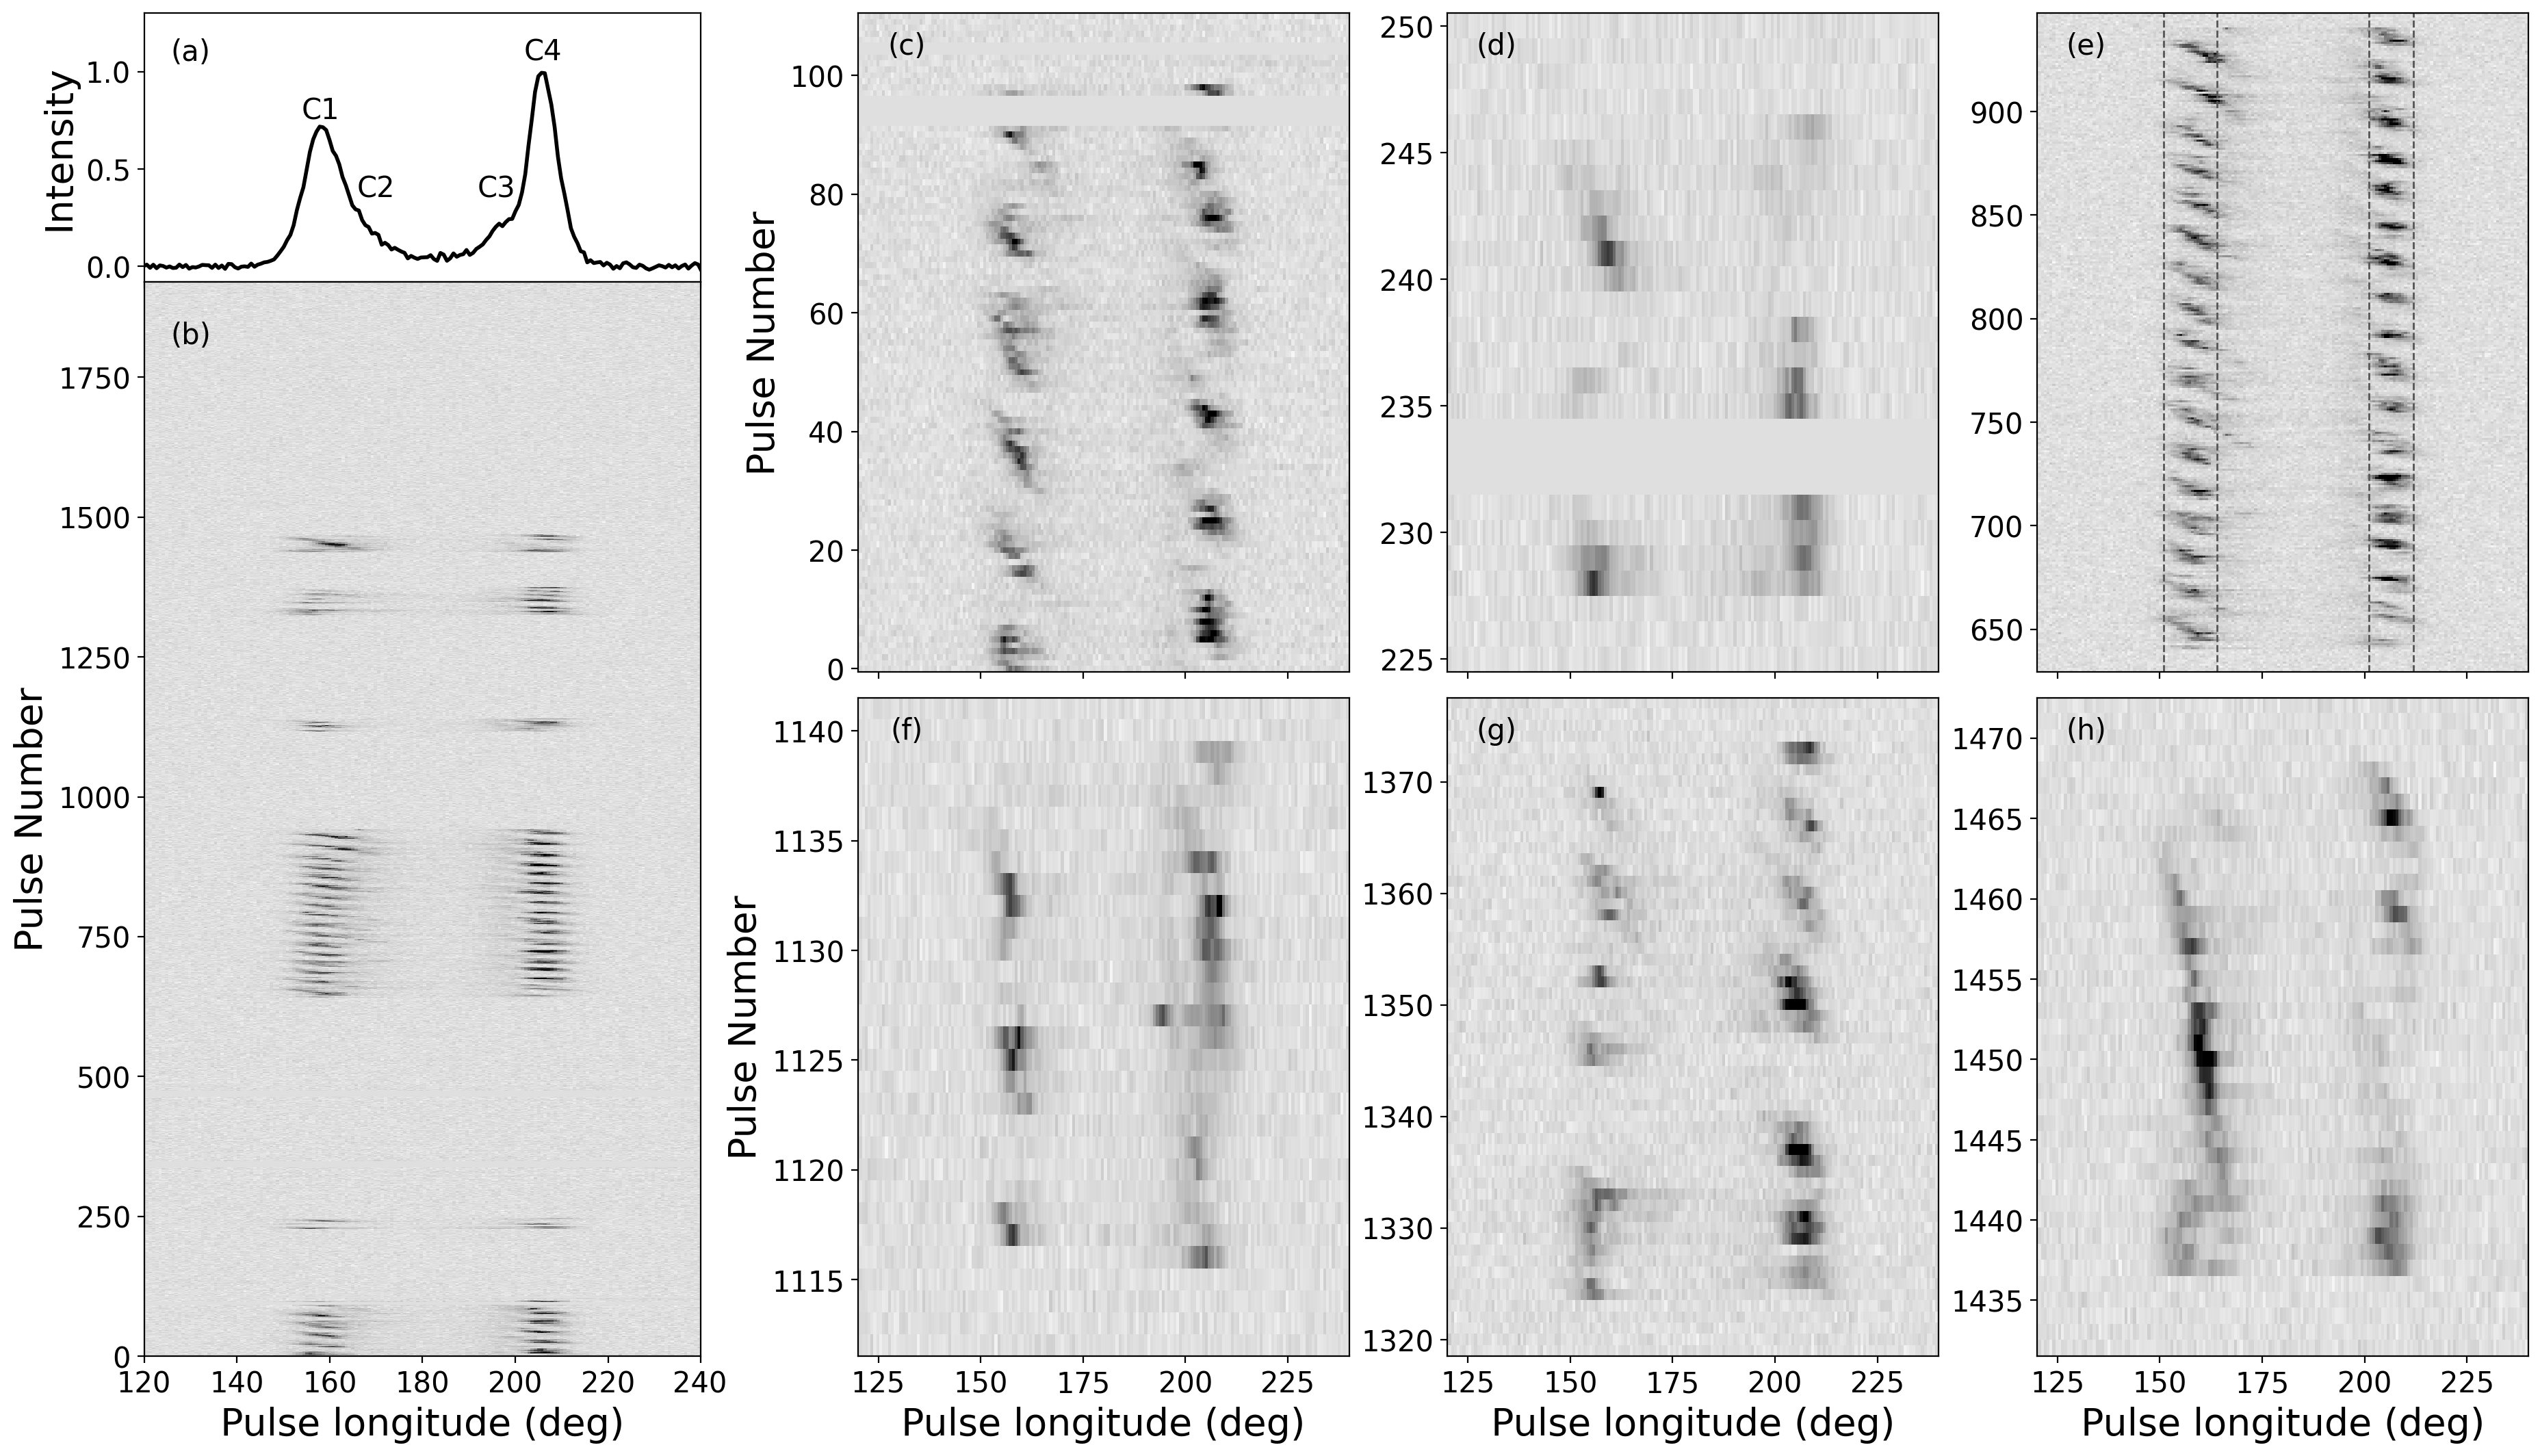
\includegraphics[height=0.8\textwidth]{Figures/J1926/stack.png}
            \caption[Pulse stacks of PSR~J1926$-$0652 as seen with FAST]{The integrated pulse profile of PSR~J1926$-$0652 averaged across the full 270 to 800~MHz band (panel (a)) with the four profile components labelled. The single pulses are shown in panel (b). The data shown is from the single, uncalibrated polarisation channel. Panels (c)--(h) show each of the six bursts present in the observation. The top three panels are bursts 1 to 3, and the lower panels are bursts 4 to 6.}
            \label{fig: J1926 - pulse stack}
        \end{center}
    \end{figure}
\end{landscape}


\subsection{Fluctuation analysis}
\label{sec: J1926 - analysis - single pulse variability}


Fourier analysis can be used to quantify subpulse modulation. Two key techniques used in this analysis are the longitude-resolved fluctuation spectrum \citep[LRFS;][]{Bxxx1970a}, and the two-dimensional fluctuation spectrum \citep[2DFS;][]{ESxx2002}. The LRFS is used to detect periodicities that occur at a given pulse longitude across a pulse stack. If periodic modulation is occurring, a given column of intensities will resemble a sinusoidal pattern with a period $P_3$, which can be detected by performing discrete Fourier transforms (DFTs) in this direction. To calculate the LRFS, the pulse stack is divided into blocks of $n$ pulses where $n$ is the chosen length of the Fourier transform to be calculated. For each block, a DFT is calculated for each column corresponding to a fixed pulse longitude bin. The number of pulses in each block must be a power of two, and the length of the DFT determines the spectral resolution. The longer the block, the higher the resolution -- however, the signal-to-noise ratio (S/N) per spectral bin will decrease. Therefore a balance must be found. In this analysis a block size of 512 pulses was used, meaning only 1536 out of the 1921 total pulses in the FAST observation were used. As no emission was detected from pulse 1469 onwards, this does not affect the results. The power spectra for the individual blocks are then averaged to produce the LRFS, which has pulse longitude on the $x$-axis, and the periodicity $P_1/P_3$ in cycles per period (cpp) is displayed on the $y$-axis. 

Similar to the LRFS, the 2DFS highlights $P_3$ periodicities, and also $P_2$ periodicities. Additional Fourier transforms are calculated in the horizontal (pulse longitude) direction of the pulse stack in order to quantify any fluctuation that occurs \textit{within} a single pulse period, such as the separation between drifting subpulses. For this purpose $m$ on-pulse longitude bins are selected, where $m$ is once again a power of two. In the 2DFS, the vertical and horizontal directions correspond to $P_1/P_3$ and $P_1/P_2$ respectively. Asymmetry in fluctuation power with respect to $P_1/P_2 = 0$ would indicate that there is a preferred drift direction for the subpulses.


Figure~\ref{fig: J1926 - fluctuation spectra} shows the fluctuation spectra for the full 270 to 800~MHz FAST observation of PSR~J1926$-$0652. The upper left plot shows the integrated pulse profile (solid line), along with the longitude-resolved modulation index (error bars). The modulation index is a measure of the variability of the intensity from pulse to pulse, and is equal to the standard deviation of the intensity divided by its the mean for a given pulse longitude bin. In this instance, the modulation index was calculated in the spectral domain alongside the LRFS and 2DFS, using the \texttt{pspec} program in \textsc{psrsalsa} \citep{Wxxx2016}. The error bars were calculated using bootstrapping, a robust statistical technique that requires no \textit{a priori} knowledge of the error distribution of the modulation index \citep[e.g.][]{WJxx2012}. In Fig.~\ref{fig: J1926 - fluctuation spectra} the modulation is strongest around the peak of the total intensity emission, close to profile components C1 and C4, and is slightly stronger in the latter. The displayed points are limited to those with a statistical significance greater than $3\sigma$. The modulation index is relatively large, and significantly larger than the modulation index shown in Fig.~12 of \citet{ZLH+2019} which peaks at 1.3. This is because in Fig.~\ref{fig: J1926 - fluctuation spectra} the calculation of the modulation index includes the effect of nulls, while in the publication the spectra of burst 3 only were shown.

\begin{figure}
    \begin{center}
        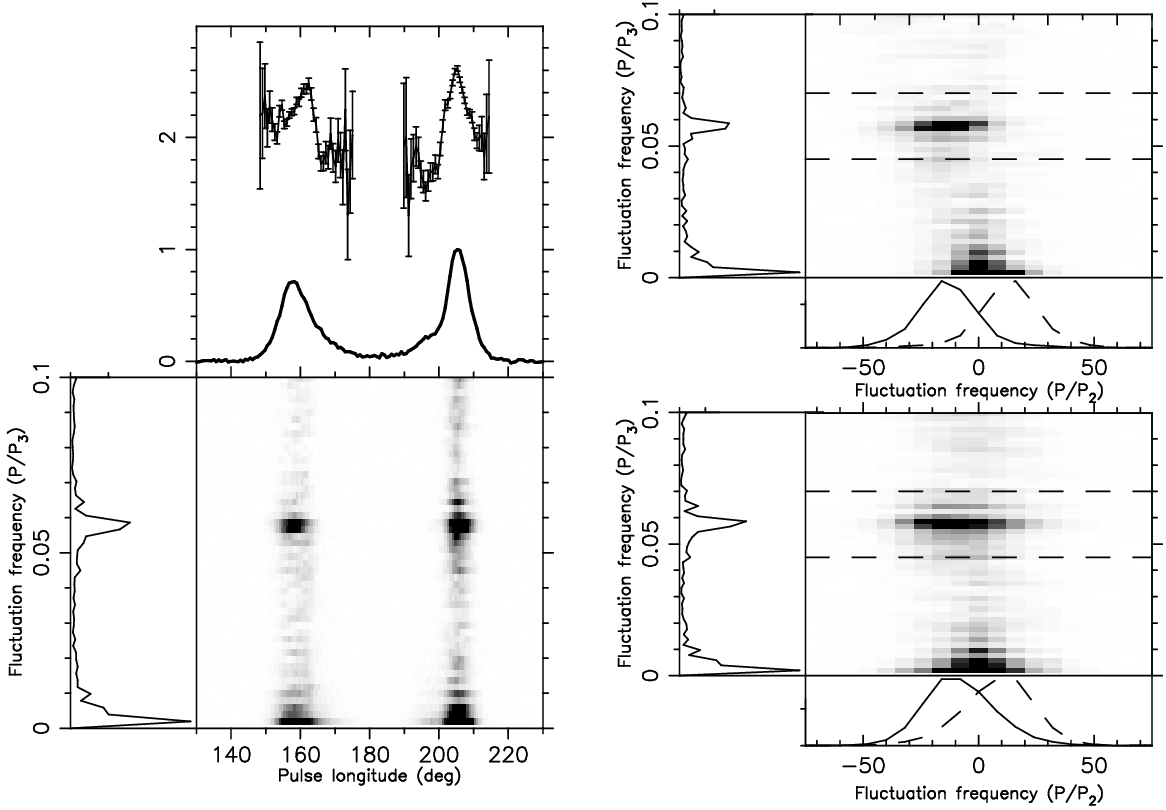
\includegraphics[width=1.0\textwidth]{Figures/J1926/fluctuation_spectra}
        \caption[LRFS and 2DFS of PSR~J1926$-$0652]{The fluctuation spectra for full FAST observation across the full frequency range of 270--800~MHz. The upper left panel shows the integrated pulse profile (solid line) and the longitude-resolved modulation index (black points with error bars). The lower left panel shows the LRFS, and the side panel is the result of integrating the power spectrum (greyscale) horizontally. The right-hand panels are the 2DFS for the leading components (upper plot) and trailing components (lower plot). Again, the left side panels of these are the result of integrating the power spectrum horizontally. The lower side plot shows the power spectrum integrated vertically between the two dashed lines (solid line). The dashed line in this panel shows the same distribution reflected about $P_1/P_2 = 0$ to highlight its asymmetry. Only part of the spectra are shown where the spectral features are strong ($0 \leq P_1/P_3 < 0.1$).}
        \label{fig: J1926 - fluctuation spectra}
    \end{center}
\end{figure}

% Describe the LRFS plot
Periodicities in the single-pulse modulation can be quantified by analysing features in the fluctuation spectra. The lower left panel of Fig~\ref{fig: J1926 - fluctuation spectra} shows the LRFS, magnified to show the on-pulse region between pulse longitudes $130\degr$ and $230\degr$. The greyscale plot shows the modulation power spectrum, and the left-hand side panel shows the spectrum integrated horizontally over the pulse window. There is a clear peak at $P_1/P_3 \simeq 0.058$~cpp for both the leading and trailing profile components, corresponding to the $P_3 \simeq 17 P_1$ periodicity in the driftbands which are clearly visible in the pulse stack (Fig.~\ref{fig: J1926 - pulse stack}). There is also an increase in spectral power visible towards $P_1/P_3 = 0$~cpp -- this is due to the nulls.

% Describe the 2DFS plots.
The two plots on the right hand side of Fig~\ref{fig: J1926 - fluctuation spectra} show the 2DFS, calculated separately for the leading half (components C1 and C2) and trailing half (components C3 and C4) in order to examine their drifting subpulses independently and to avoid the appearance of distortions in the spectra caused by non-linearity in how the driftbands in the two halves of the profile connect (see Sec.~\ref{sec: J1926 - analysis - phase tracks}). As with the LRFS, the features at $P_1/P_3 \simeq 0.058$~are clearly visible, and both have a clear offset from $P_1/P_2 = 0$ as highlighted in the lower line plots. In this panel, the solid line shows the power spectrum integrated vertically in the region of interest bounded by the horizontal dashed lines. In order to highlight the asymmetry of this distribution, it was reflected about $P_1/P_2 = 0$ and this is shown by the dashed line in the lower panels. The centroids of the spectral features were measured using the \texttt{pspecDetect} program in \textsc{psrsalsa} and the measured periodicities are $P_3 = (17.39 \pm 0.07)P_1$ and $P_2 = (25.5 \pm 0.4)\degr$ for components C1 and C2, and $P_3 = (17.33 \pm 0.09)P_1$ and $P_2 = (42\pm 1)\degr$ for components C3 and C4. These measurements are consistent with those presented in \citet{ZLH+2019} where burst 3 only was analysed. These values correspond to drift rates of $D = P_2 / P_3 = (1.47 \pm 0.02)\degr/P_1$ and $D = (2.42 \pm 0.06)\degr/P_1$ respectively. This quantifies the difference in the driftband gradients between the two halves of the profile that is clearly visible in Fig.~\ref{fig: J1926 - pulse stack}, especially for burst 3 (panel (e)). These values represent the \textit{average} drift properties across the full pulse stack -- the uncertainties quoted do not fully account for the large variability in the driftband shapes, or how they may change between different bursts. The lengths of the bursts are too short to reliably quantify their drift properties individually. The results for $P_3$ for the leading and trailing halves are consistent with one another, as expected if the drifting subpulses are produced by a circulating carousel (see Chapter~\ref{chapt: B0031}).




\subsection{\texorpdfstring{$P_3$}{P3} folding}
\label{sec: J1926 - analysis - P3 folding}

In order to more clearly see the average drift band structure in PSR~J1926$-$0652, the technique of $P_3$-folding was used, as described in Sec.~\ref{sec: intro - emission models - single pulse phenomena - P3 folding}. For PSR~J1926$-$0652, $P_3$ is highly variable, as can be seen in the irregular spacing of drift bands in bursts four to six in Figure \ref{fig: J1926 - pulse stack}. Burst 3 appears relatively stable and is the longest continuous time in which the emission was detected, and so this burst was chosen for $P_3$ folding. The last few driftbands were excluded as they have visually different shapes. As well as the full 270 to 800~MHz band, three frequency sub-bands spanning 270--400~MHz, 400--600~MHz, and 600--800~MHz were also analysed. A $P_3$-fold was formed for each sub-band as well as the full frequency range in order to study if and how the drift bands evolve with frequency. This was achieved by first folding the full frequency pulse stack with a periodicity $P_3 = 17.36P_1$ as this dataset has the highest S/N. Since $P_3$ is somewhat variable, phase offsets were allowed between blocks of 17 pulses. These phases, obtained by performing cross-correlations between the blocks of data, were recorded. The same phase offsets were used to fold the sub-band pulse stacks without doing any further fitting. In this manner, the $P_3$-folds are perfectly aligned and folded identically, permitting a meaningful comparison.

\begin{figure}
    \begin{center}
        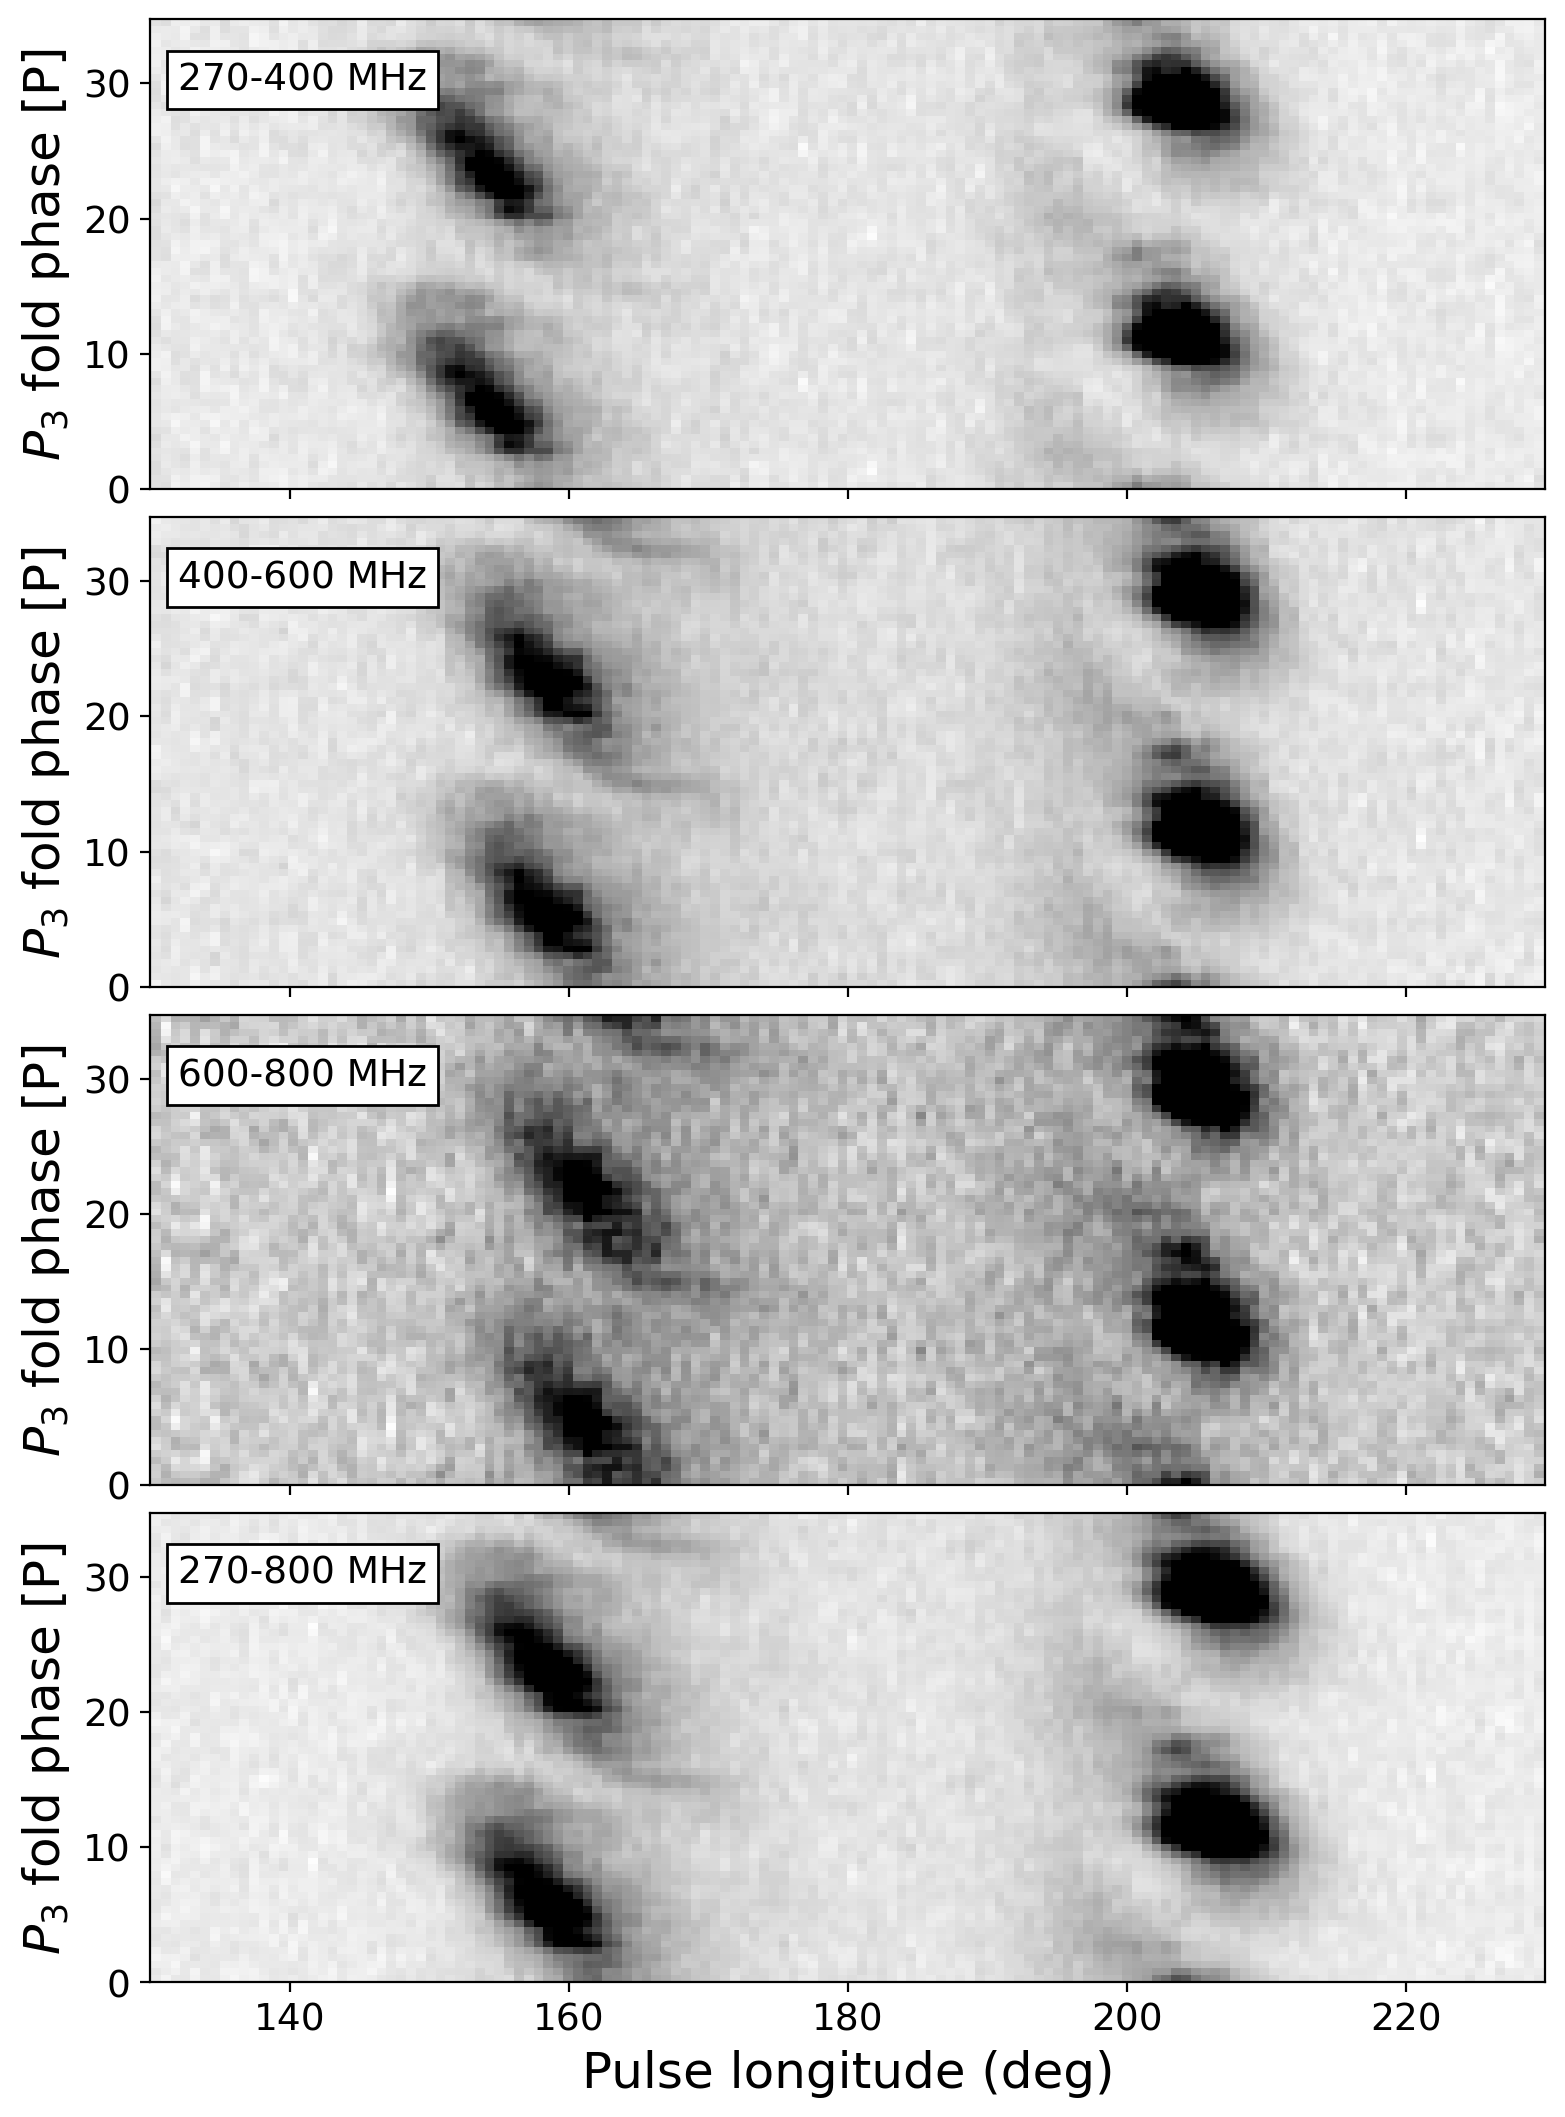
\includegraphics[width=0.8\textwidth]{Figures/J1926/p3_folds3}
        \caption[The average drift bands of PSR~J1926$-$0652 at different frequencies.]{A comparison of the average drift band obtained by $P_3$-folding the data of burst 3 at three different frequency bands. The top panel spans 270--400~MHz, the second panel spans 400--600~MHz, and the third panel spans 600--800~MHz. The bottom panel shows the average drift band across the combined frequency range of 270--800~MHz. The intensity has been clipped to 30~per~cent of its peak to highlight the fainter, inner structures.}
        \label{fig: J1926 - p3 folds}
    \end{center}
\end{figure}

The four $P_3$-folds are shown in Figure \ref{fig: J1926 - p3 folds}, with the bottom panel being identical to the $P_3$-fold shown in Fig.~11 of \citet{ZLH+2019}. The sub-bands are plotted vertically beginning with the lowest frequency band at the top. The $P_3$-fold for the full frequency range is shown at the bottom. For clarity, each set of driftbands is plotted twice in order to show the continuity of the emission, and in order to better show the much weaker inner components the intensity has been clipped to 30~per~cent of its peak in each sub-band.  It is clear from the movement of the leading component to later pulse longitudes that the profile width decreases at higher frequencies, which is to be expected due to the narrowing of the emission region as described by radius to frequency mapping \citep[e.g.][]{Cxxx1978}. The two inner components (C2 and C3) are slightly more visible at higher frequencies, albeit still faint compared to the regions associated with profile components C1 and C4. In the leading half of the profile, the extra component appears as a small tail on the driftband at longitudes between $160\degr$ and $170\degr$ around a $P_3$-fold phase of 17, and is most visible in the 600--800~MHz sub-band -- this is component C2. Similarly an extension to the driftband appears in the trailing half, extending the emission to earlier pulse longitudes -- component C3. Here, the emission associated with C3 appears to be brightest between the main drift bands in $P_3$-phase, appearing between phases 17 and 26 at longitudes $195\degr$ and later. This discontinuity in the otherwise linear driftbands suggests that a single carousel is not enough to explain these observations. Subpulse phase tracks will be used next to quantify this discontinuity further. The analysis of the $P_3$-folds show that the profile shape is frequency-dependent in terms of both the location of the components and their spectral indices.


% This apparent phase jump suggests an extra patch of emission may be responsible rather than a continuation of the main patch which forms the bright feature at $205\degr$. The $P_3$-folds provide one way of analysing the average drifting behaviour in PSR~J1926$-$0652, but are still confused by the presence of noise and bright features which dominate the low-intensity emission in the central bridge region. Therefore, an alternative analysis is required.


\subsection{Subpulse phase tracks}
\label{sec: J1926 - analysis - phase tracks}

The shape of the average driftbands can be quantified with the so-called `subpulse phase' as a function of pulse longitude. It is particularly useful for quantifying discontinuities and curvature in driftbands. The subpulse phase track follows from Fourier analysis, similar to that used to compute the LRFS and 2DFS (see Sec.~\ref{sec: J1926 - analysis - single pulse variability}). The pulse stack is divided into blocks of length defined by the length of the discrete Fourier transform (DFT) to be used. DFTs are calculated for each pulse longitude bin independently.

The DFT is calculated over a list of $N$ intensities $a_n$ according to
\begin{equation}
    A_k = \sum^{N-1}_{n=0} a_n e^{-i2\pi \frac{kn}{N}}.
\end{equation}
Here $N$ is the length of the DFT (the length of the block in the pulse stack, and a power of two), $n$ is the index of a given sample starting at $0$, and $k$ is the index of the corresponding sample in the resulting Fourier transform output. The sequence $A_k$ is the DFT of the time series of flux densities $a_n$, where $A_k$ are complex numbers. Their amplitudes quantify how strong the frequency $k$ contributes to the signal, and the complex phase offset is that required to make a sinusoid with frequency $k$ match the time series. 

The modulation frequency $k$ is chosen to correspond to the $P_3$ period of the drifting subpulses as identified from the LRFS. The amplitude and complex phase of $A_k$ are calculated for all pulse longitudes independently. For linear driftbands the phase will change linearly with pulse longitude. We define the subpulse phase to have the opposite sign compared to the complex phase -- this ensures that an increasing subpulse phase with pulse longitude corresponds to positive drifting, i.e. subpulses that appear later at later longitudes. This means that the sight of the gradient of the subpulse phase track is identical to the gradient of the drifting subpulses in the pulse stack. Furthermore, the amplitude of $A_k$ can be considered as a function of pulse longitude, which quantifies how the intensity of the drifting subpulses change across the pulse window.

% discrete Fourier transform of the sequence $a_n$, each being a list of $N$ numbers. Each $A_k$ is a complex number. The amplitude corresponds to the strength of the modulation, and the phase corresponds to the phase of a sinusoid with frequency $k$ which matches the data.

% In practice, the modulation frequency $k$ is chosen by selecting a $P_3$ spectral bin of interest from the LRFS -- a sensible selection would be the peak value. The magnitude and phase of this modulation are calculated for all pulse longitudes independently. For linear driftbands the phase (subpulse phase) will change linearly with pulse longitude. Plotting the magnitude of the modulation as a function of pulse longitude gives an idea of how the driftbands change in intensity across the pulse window.

As well as burst 3 the most stable pattern of drifting occurs in burst 1, as can be seen in Fig.~\ref{fig: J1926 - pulse stack}. Bursts 1 and 3 lie within the pulse number ranges 0--94 and 641--930 respectively in the pulse stack, which means that the maximum DFT length for burst 1 is 64, and for burst 3 is 256. As shown earlier, the average modulation period for PSR~J1926$-$0652 is $P_3 = (17.4 \pm 0.1)P_1$ which corresponds to a frequency of $\sim$0.058~cpp. The closest spectral bin was selected for the two bursts.

\begin{figure}
    \begin{center}
        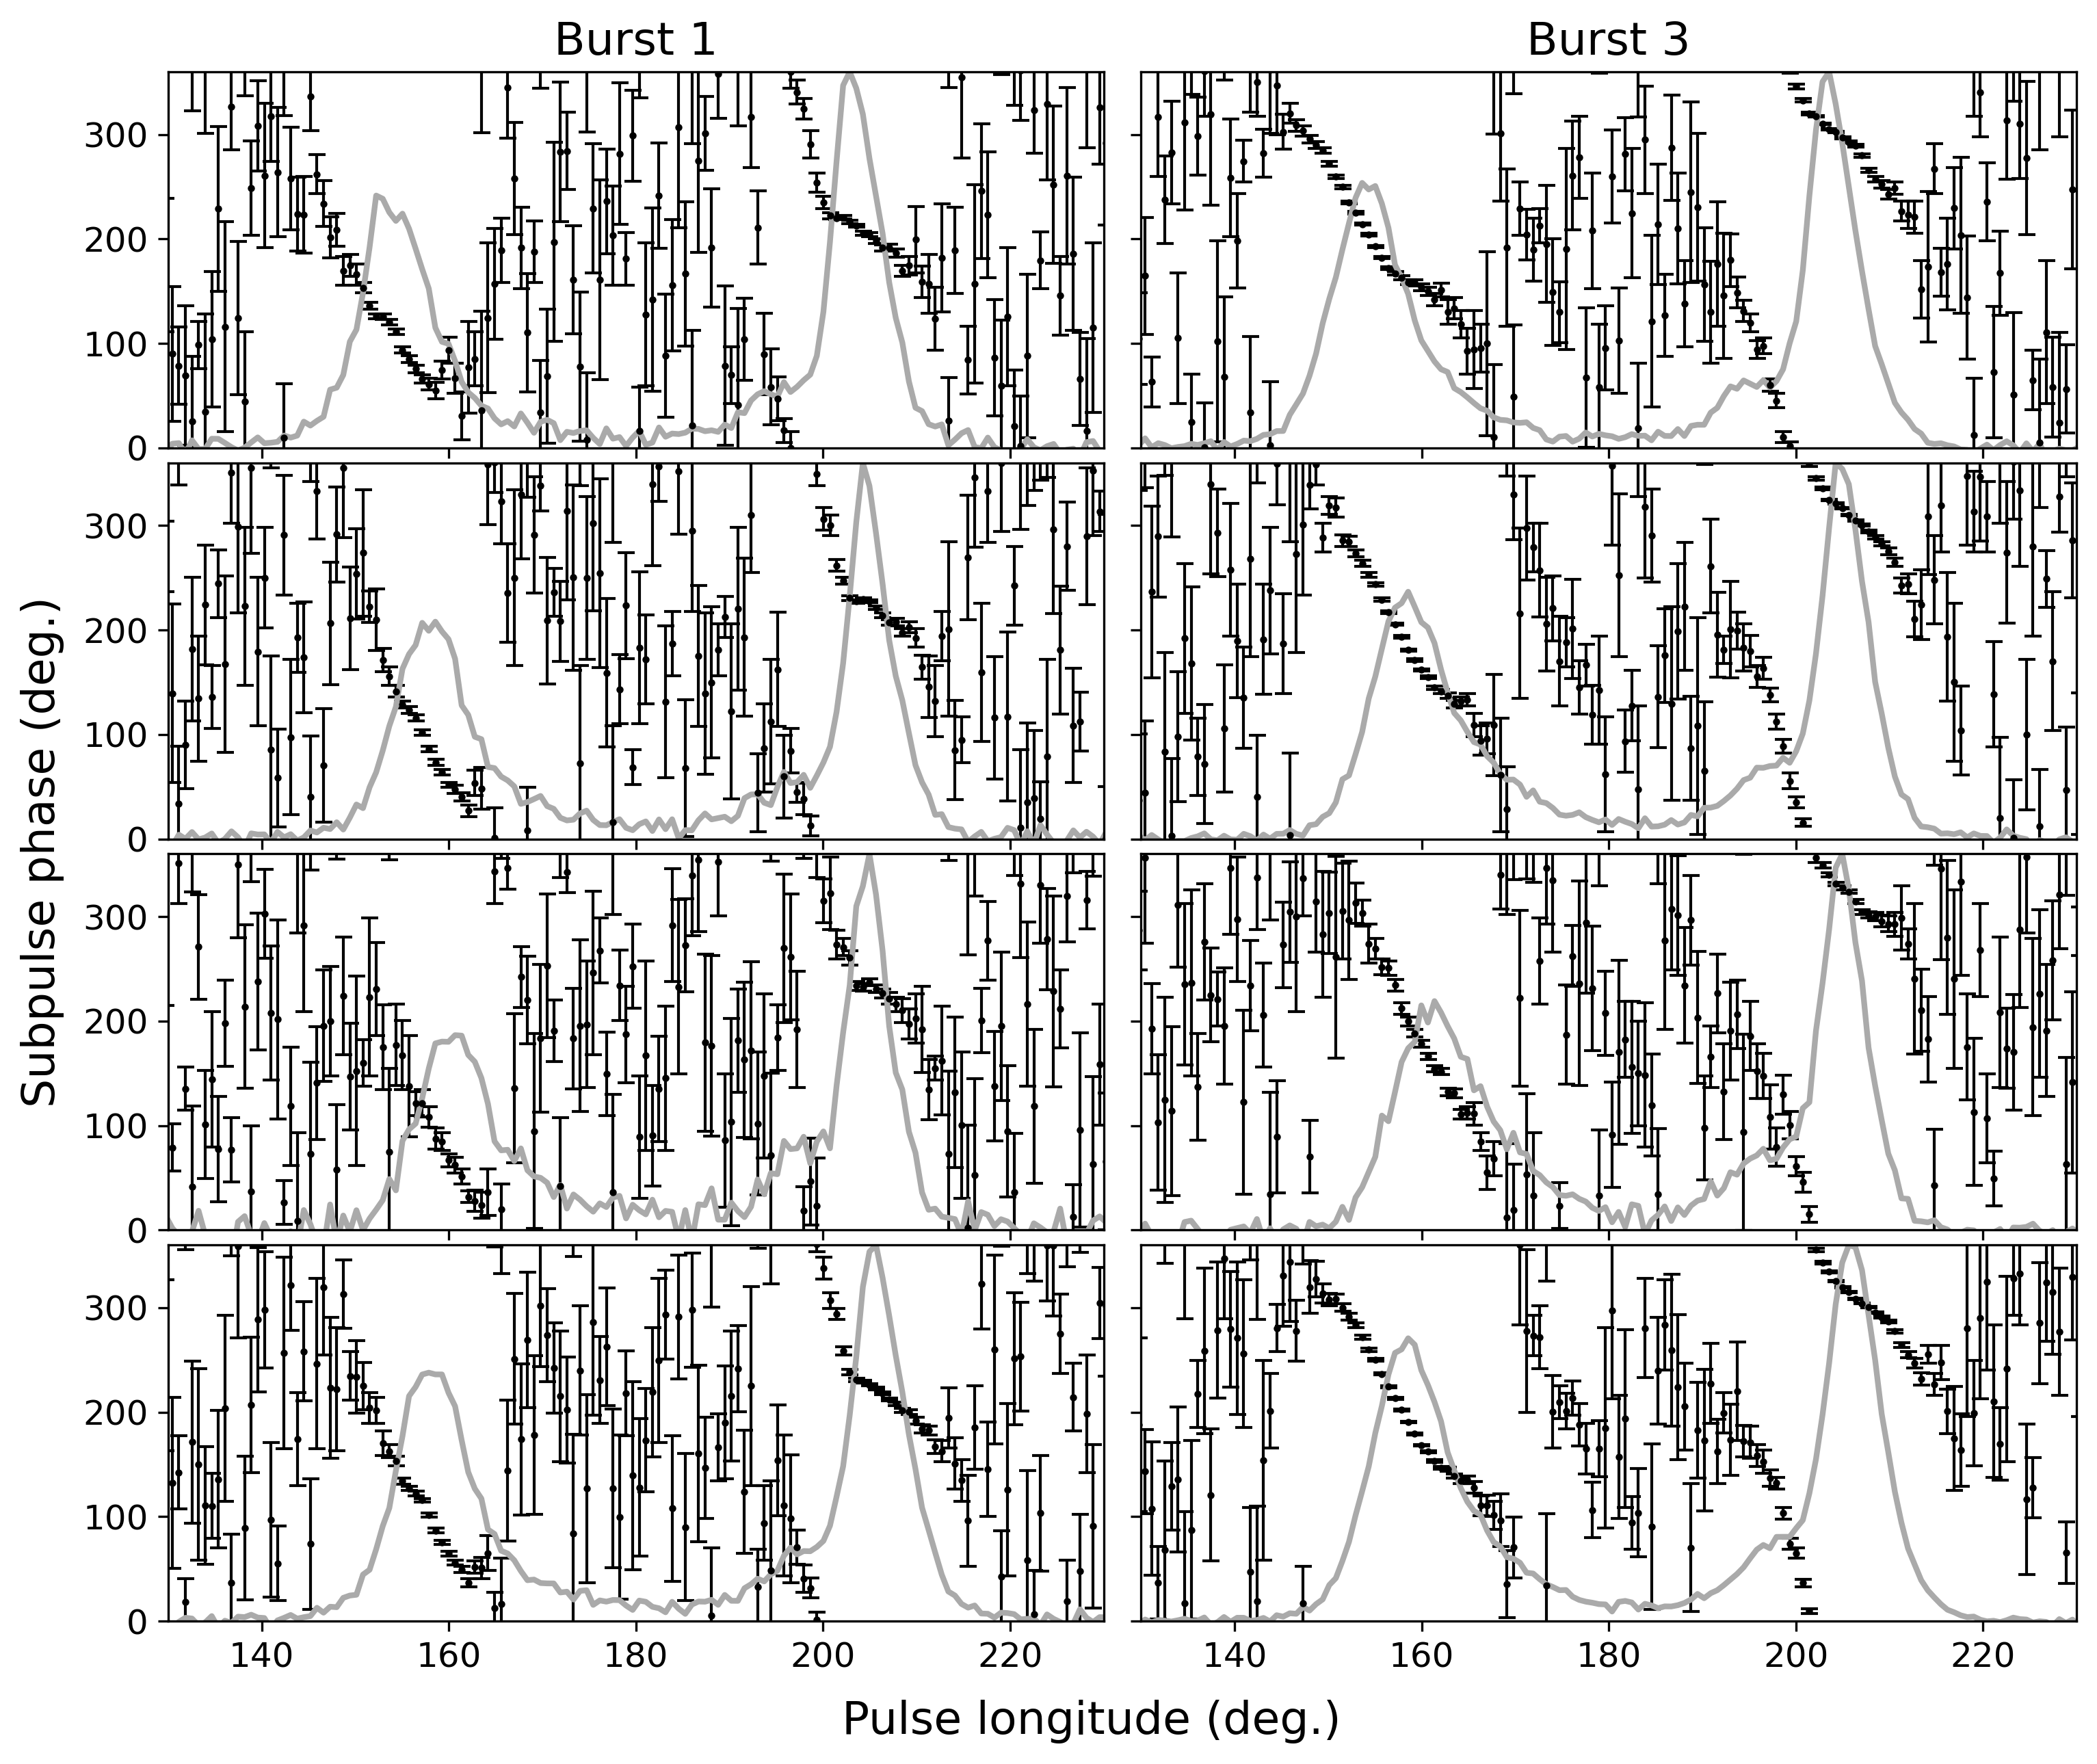
\includegraphics[width=1.0\textwidth]{Figures/J1926/subpulse_phase}
        \caption[Subpulse phase tracks of PSR~J1926$-$0652]{A comparison of the subpulse phase tracks of bursts 1 (left column) and 3 (right column) at three different frequency bands. As for Fig.~\ref{fig: J1926 - p3 folds}, the top panels span 270--400~MHz, the second panels span 400--600~MHz, and the third panels span 600--800~MHz, while the bottom panels correspond to the entire frequency range of 270--800~MHz. The grey line shows the integrated profile for each burst at each frequency, while the black points with error bars show the longitude-resolved subpulse phase.}
        \label{fig: J1926 - phase tracks}
    \end{center}
\end{figure}

The subpulse phase tracks were calculated separately for each sub-band, for both burst 1 and burst 3 as shown in Fig.~\ref{fig: J1926 - phase tracks}. The left hand column shows the results for burst 1, and the right shows the results for burst 3. As in Fig.~\ref{fig: J1926 - p3 folds}, the sub-bands are shown in order of increasing frequency with the 270--400~MHz band at the top. The bottom row shows the results for the full frequency range of 270--800~MHz. Within each panel the integrated profile for the burst is shown by the pale grey line. The subpulse phase track is shown by the black points with error bars. These error bars were calculated using bootstrapping, where white noise was added to the data with a standard deviation determined from the off-pulse region for each dataset. The phase track was recalculated for one thousand iterations. For each pulse longitude there is then a distribution of subpulse phases: the standard deviation of these was taken as the uncertainty on the measurement.

For both bursts broadly similar results are obtained, although burst 3 has an overall higher S/N because of its greater length. In the leading half of the profile the phase track is continuous and reasonably straight, with an almost constant negative gradient. Towards lower frequencies a slight kink becomes visible at $\sim$150$\degr$, coinciding with the peak of the C1 profile component. The kink appears to occur earlier than the boundary between the C1 and C2 components. In contrast, the phase track in the trailing half of the profile shows a distinct discontinuity in its gradient at the boundary between the C3 and C4 profile components. In the pulse longitude range associated with C4 the phase track has a gradient comparable to that of the leading half, and becoming steeper towards the trailing shoulder of the profile. However, at the earlier longitudes corresponding to the C3 profile component the gradient of the phase track is considerably steeper still. The track wraps fully around the phase boundary at $360\degr$, which implies that for some pulses two subpulses corresponding to successive driftbands are observable. This can indeed be seen in Fig.~\ref{fig: J1926 - p3 folds}. Some structure is faintly visible in the bridge region, although the uncertainties on these points are much higher. Kinks and other unusual features in phase tracks have previously been seen in other pulsars -- their interpretation is discussed in Sec.~\ref{sec: J1926 - discuss - phase track}.

A form of Fourier analysis analogous to subpulse phase tracks was conducted by \citet{ZLH+2019}, which gave very similar results to those discussed here. In addition, to explore the variability in $P_3$, the subpulses were tracked on an individual pulse basis. This was achieved by fitting a single Gaussian to the intensity in the leading half (profile components C1 and C2), and another to the trailing half (profile components C3 and C4). The centroids of the Gaussians were measured, and then a weighted straight-line fit was performed for each driftband to determine the drift rate $P_2/P_3$. The driftband slopes found using this method are systematically different to those found by the Fourier analysis, giving somewhat steeper driftbands. The benefit of this method is that each driftband is treated independently, meaning that it is better equipped to deal with variability in $P_3$, whereas the Fourier analysis effectively assumes it is constant over the course of the observation. This method can also be applied to the shorter bursts where the Fourier analysis would have insufficient frequency resolution (a longer FFT could be used, but risks becoming contaminated by the nulls or other neighbouring bursts). However, the downside to the Gaussian fitting method is that it is somewhat subjective as to which subpulse structures are used, especially when there are multiple subpulses present in a given component (e.g. both C1 and C2 driftbands can be seen around pulse numbers 704 and 738). The driftbands are also assumed to be fitted by straight lines, which is not necessarily accurate. Overall, both methods have their strengths, but unless the drifting is regular they can lead to different results.











\subsection{Polarisation properties}
\label{sec: J1926 - analysis - polarisation}

The follow-up data from the Parkes telescope in Australia, which was used for long term timing of PSR~J1926$-$0652, could be used to perform reliable polarimetric analysis. The calibrated data of the different observations were summed to create a polarised integrated profile using the \textsc{psrchive} software \citep{HSMx2004} and this was then further analysed using \textsc{psrsalsa}. The program \texttt{ppol} was used to calculate the polarised profile shown in Figure \ref{fig: J1926 - parkes profile}.
\begin{figure}
    \begin{center}
        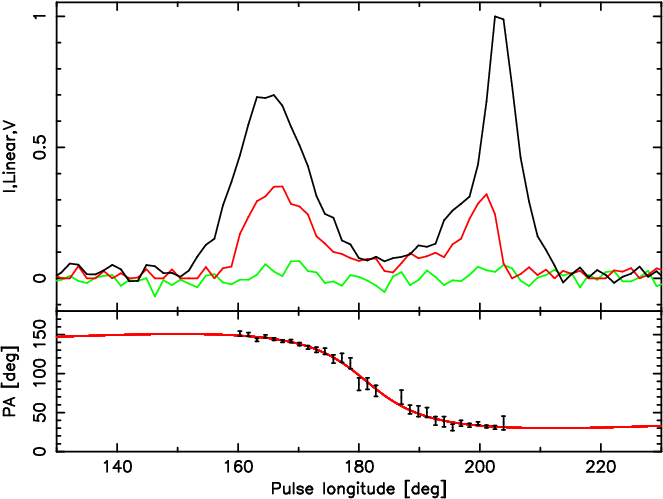
\includegraphics[width=0.6\textwidth]{Figures/J1926/parkes_profile}
        \caption[The polarised profile as observed with Parkes]{The polarised profile of PSR~J1926$-$0652 as it was observed with the Parkes telescope. In the upper panel the black, red, and green lines show the total intensity, linear polarisation, and circular polarisation respectively. In the lower panel the points show the PA as a function of pulse longitude, fitted by the RVM (red curve).}
        \label{fig: J1926 - parkes profile}
    \end{center}
\end{figure}
In the upper panel the normalised total intensity $I$ profile is shown by the solid black curve, and the linearly polarised intensity $L$ is shown by the red curve. There is a negligible amount of circularly polarised emission $V$, as indicated by the green line. The fractional linear polarisation is moderate at $(38\pm1)$~per~cent and was de-biased according to \citet{WKxx1974}, and there is little evidence for significant circular polarisation. The lower panel shows the position angle of linear polarisation (PA) as a function of pulse longitude (black points). The uncertainty on the PA arises from the measurement errors on the Stokes parameters, which are Gaussian-distributed with equal standard deviations such that $\sigma_I = \sigma_Q = \sigma_U = \sigma_V$. The PA is given by $\psi = 0.5\arctan(U/Q)$ (see Sec.~\ref{sec: intro - emission models - polarisation}), so from standard error propagation its uncertainty is
\begin{equation}
    \label{eq: J1926 - PA uncertainty}
    \sigma_\psi = \frac{1}{2L^2}\sqrt{U^2\sigma_Q^2 + Q^2\sigma_U^2} \simeq \frac{\sigma_I}{2L},
\end{equation}
where $L^2 = Q^2 + U^2$. In reality the errors on $\psi$ are non-Gaussian due to its cyclic nature, and so normal error propagation is not strictly valid -- this was explored in detail by \citet{NCxx1993}. Equation~\eqref{eq: J1926 - PA uncertainty} is a good approximation if $L$ is highly significant; in Fig.~\ref{fig: J1926 - parkes profile} the displayed PA points are limited to those in which $L$ is at least twice the off-pulse root mean square of $I$, and so the calculated uncertainties are reliable.

As explained in Sec.~\ref{sec: intro - emission models - polarisation - RVM}, according to the RVM the PA in radio pulsars is indicative of the orientation of the magnetic field lines where the emission was produced \citep{RCxx1969}. The RVM predicts the PA to have a characteristic S-shaped curve as a function of pulse longitude. The RVM is parametrised by the magnetic inclination angle, $\alpha$, and line-of-sight impact parameter $\beta$ with respect to the magnetic axis, and has an inflection point at ($\phi_0$, $\psi_0$). In full,
\begin{equation}
    \tan(\psi - \psi_0) = \frac{\sin(\phi-\phi_0)\sin\alpha}{\sin(\alpha+\beta)\cos\alpha-\cos(\alpha+\beta)\sin\alpha\cos(\phi-\phi_0)}.
    \label{eq: J1926 - RVM}
\end{equation}

Fitting Eq.~\eqref{eq: J1926 - RVM} to the observed PA was achieved by performing a grid search over $\alpha$ and $\beta$, and then optimising the free parameters $\psi_0$ and $\phi_0$ by minimising the $\chi^2$ fit of the observed PA. A second program from {\sc psrsalsa}, \texttt{ppolFit} was used to achieve this. The parameters $\phi_0$ and $\psi_0$ were initially estimated by eye from the shape of the PA curve, and then optimised using the downhill simplex method \citep{NumericalRecipes}. This minimisation process was then repeated across the grid of $\alpha$ and $\beta$ values. The optimum fit is shown as the red curve in the bottom panel of Fig.~\ref{fig: J1926 - parkes profile} which is a good fit to the data, confirmed by the reduced-$\chi^2$ of 0.8.
\begin{figure}
    \begin{center}
        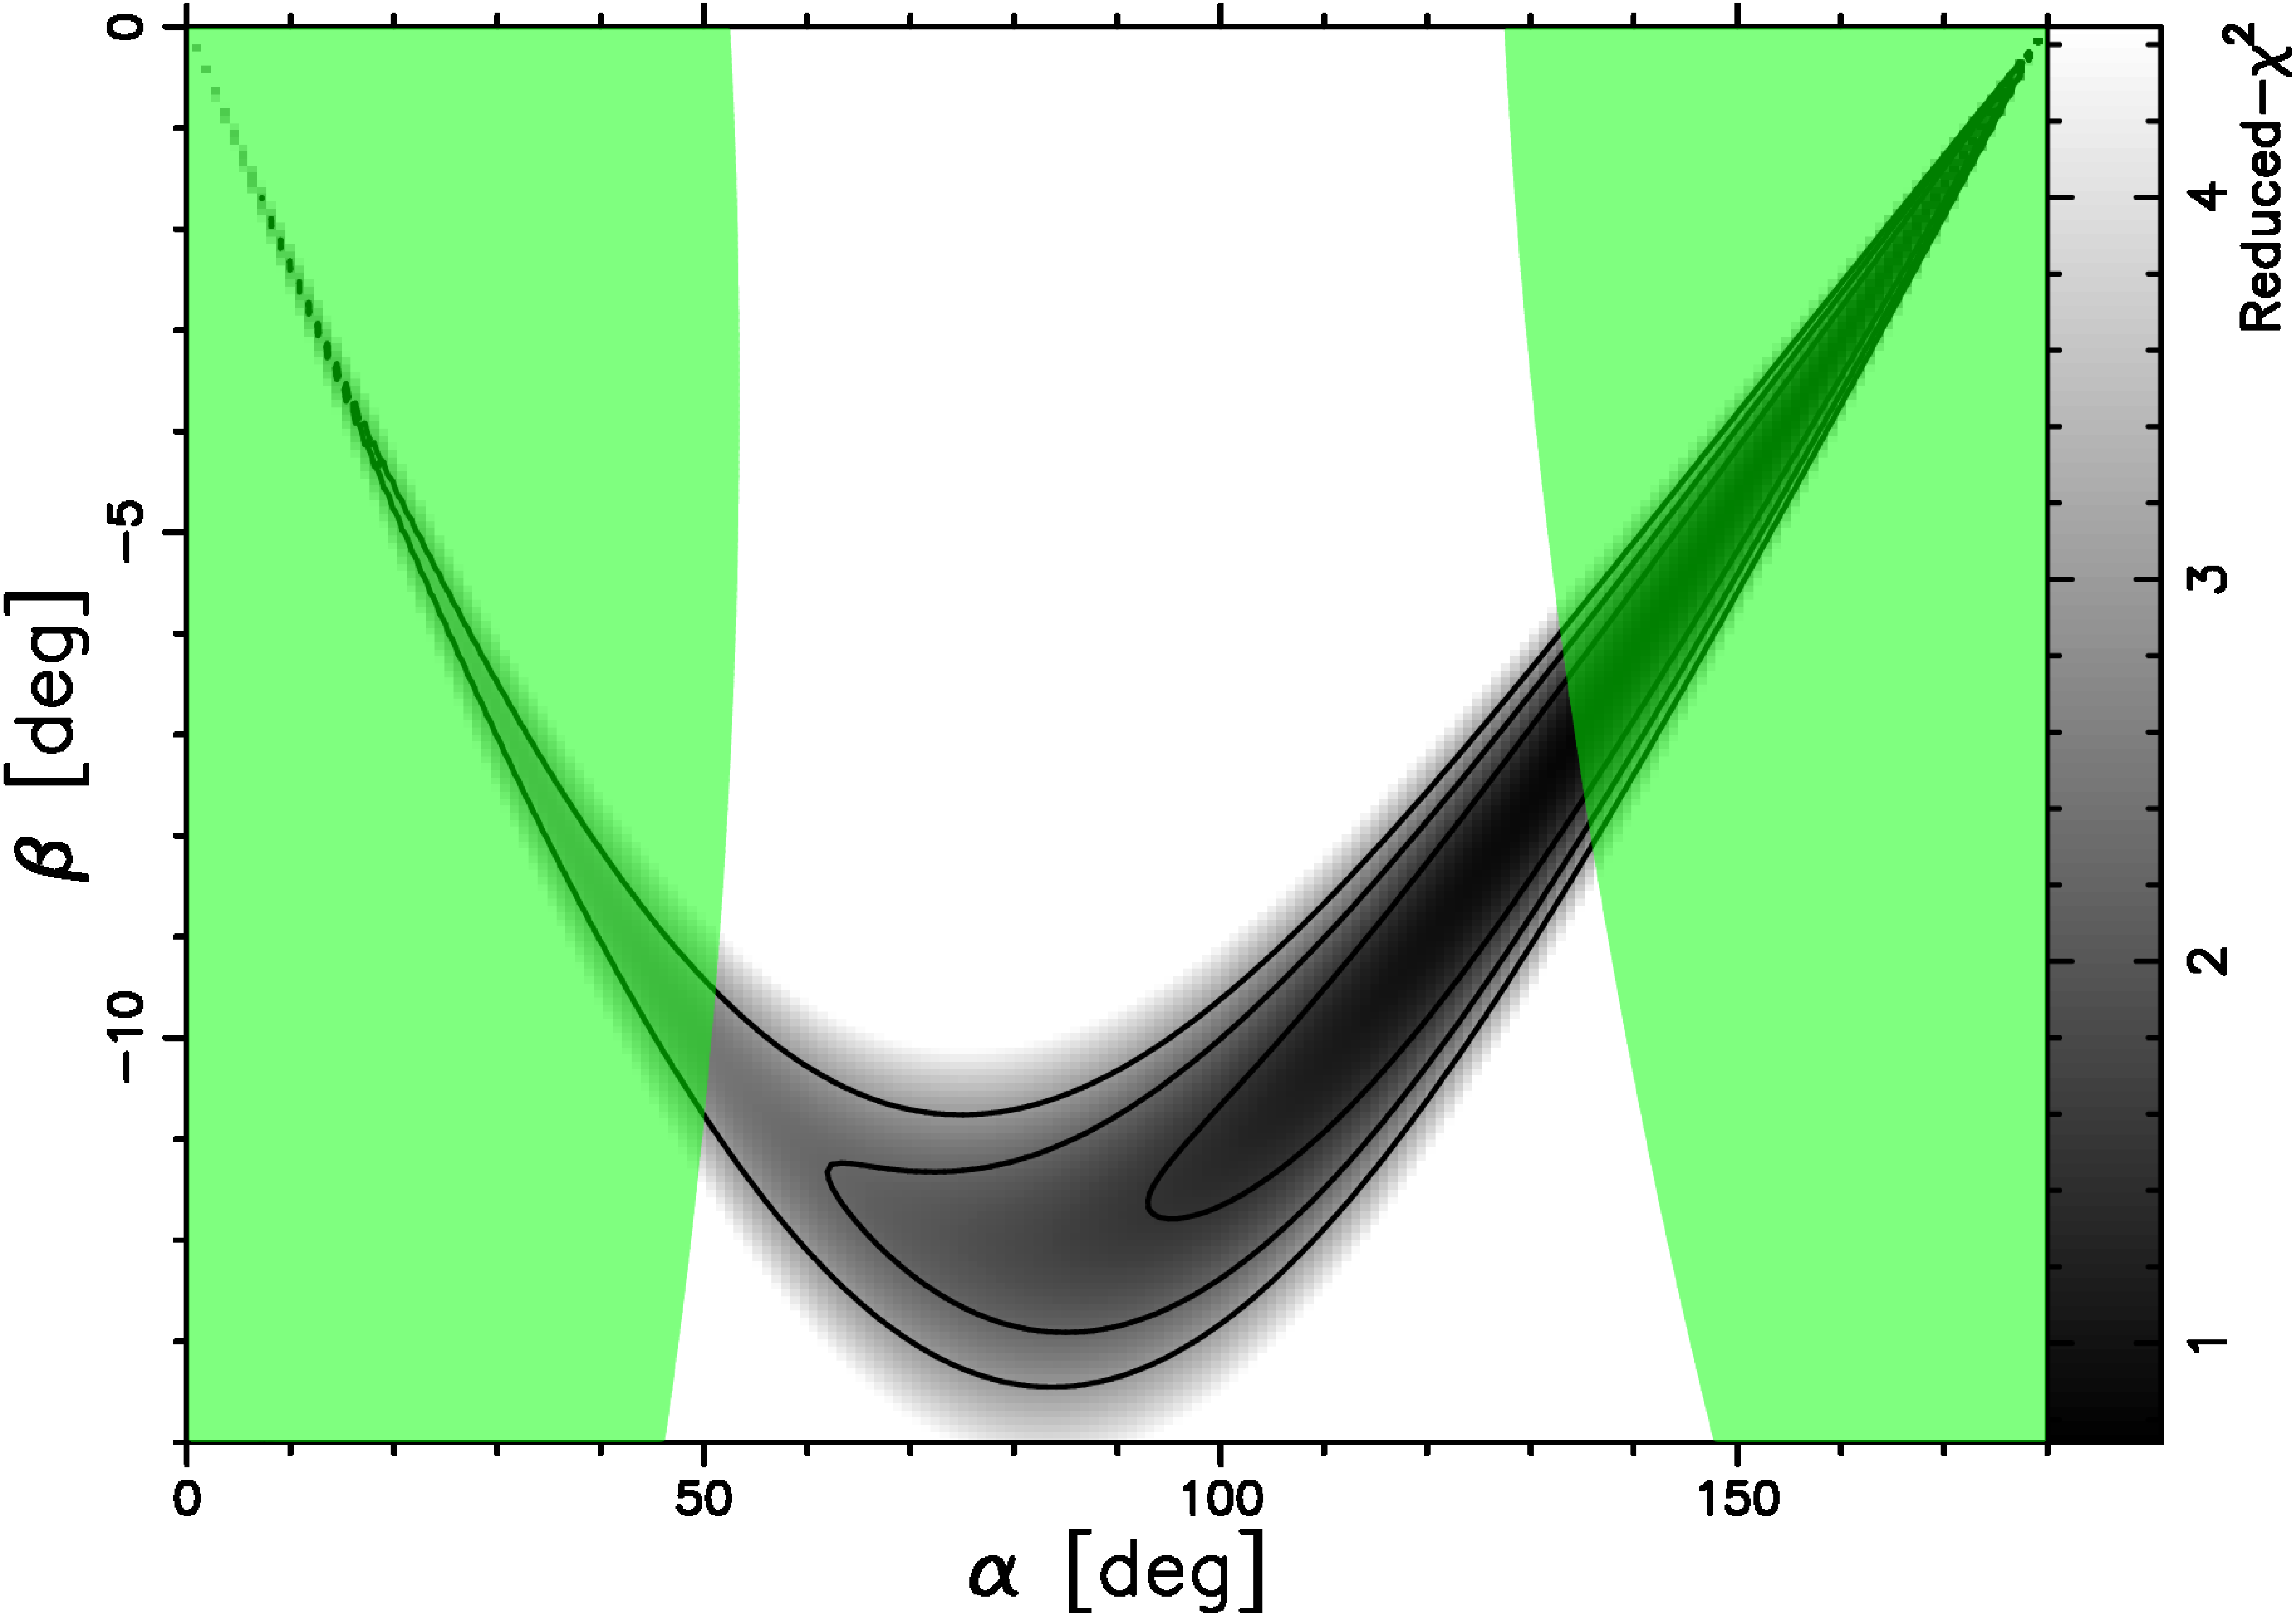
\includegraphics[width=0.7\textwidth]{Figures/J1926/banana_plot}
        \caption[The goodness-of-fit of the RVM to the PA curve]{The results of fitting the RVM across a grid of $\alpha$ and $\beta$ values. The greyscale indicates the reduced-$\chi^2$. The contour lines represent $1\sigma$, $2\sigma$, and $3\sigma$ confidence intervals corresponding to two, three, and four times the lowest reduced-$\chi^2$. The green regions indicate `allowed geometries' based on the observed profile width.}
        \label{fig: J1926 - banana plot}
    \end{center}
\end{figure}

There is no single solution of the RVM that fits the data satisfactorily, as shown by the distribution of reduced-$\chi^2$ across ($\alpha$, $\beta$) space (Fig.~\ref{fig: J1926 - banana plot}). This shows that despite the fit being very good, $\alpha$ is practically unconstrained by the RVM. The impact parameter is constrained to $|\beta| \lesssim 14^\circ$.

Further constraints can be placed upon the viewing geometry by taking into account the observed profile width, using the method of \citet{RWJx2015a}. The width of the pulse profile is governed by how the observer's line of sight (LOS) intersects the emission beam, which is determined by $\alpha$ and $\beta$. \citet{GGRx1984} showed that the pulse longitude range $W$ (the pulse width) for which the LOS intersects the open-field-line region is given by 
\begin{equation}
    \label{eq: J1926 - allowed geometry}
    \cos\rho = \cos\alpha\cos(\alpha+\beta)+\sin\alpha\sin(\alpha+\beta)\cos\bigg(\frac{W}{2}\bigg),
\end{equation}
where $\rho$ is the half opening angle of the cone of radio emission. The opening angle of the emission cone is delimited by tangents to the last open field lines at the height at which emission is produced, $h_\mathrm{em}$. However, it should be noted that the open-field-line region does not necessarily produce emission over its full area \citep[e.g][]{LMxx1988}, and so the measured profile width may not necessarily correspond to the full extent of the open-field-line region. At low emission altitudes $h_\mathrm{em} \ll R_\mathrm{LC}$, the small angle limit applies \citep[e.g.][]{Gxxx1981,KDxx1983,Rxxx1990} and the half opening angle of this cone defined by the open-field-line region is given by
\begin{equation}
    \label{eq: J1926 - emission cone angle}
    \rho \approx \sqrt{\frac{9\pi h_\mathrm{em}}{2cP}}.
\end{equation} 
The combination of Eqs.~\eqref{eq: J1926 - allowed geometry} and \eqref{eq: J1926 - emission cone angle} implies that for a given $\alpha$ and $\beta$, pulsars with a greater emission height will produce wider profiles because of the diverging dipole field. The emission height also has an effect on the polarisation properties of the pulse profile, through relativistic aberration and retardation (A/R) effects which cause the inflection point of the RVM curve (Eq.~\eqref{eq: J1926 - RVM}) to move to later pulse longitudes, whilst the total intensity profile appears to shift earlier. \citet{BCWx1991} showed that the expected delay in pulse longitude between the fiducial plane and the RVM inflection point is $\Delta\phi = 4h_\mathrm{em}/R_\mathrm{LC}$, where $R_\mathrm{LC}$ is the size of the light cylinder (see Sec.~\ref{sec: intro - general intro}). By measuring this delay, the emission height can be estimated.

As seen in Fig.~\ref{fig: J1926 - parkes profile}, the inflection point of the RVM curve fitted to the PA data lies close to the centre of the profile of PSR~J1926$-$0652, which has a `conal-double' morphology \citep[][]{Rxxx1983a}. The shift due to A/R effects is believed to be no more than $\sim$14$\degr$, implying an emission height of less than 5000~km. This is presented as an upper limit due to the uncertainty on the location of the fiducial plane of the total intensity profile, which is somewhat asymmetric with the leading half being much broader than the trailing half. Furthermore, the location of the inflection point of the fitted RVM curve was found to vary by $8\degr$ in pulse longitude within the $3\sigma$ confidence region indicated in Fig.~\ref{fig: J1926 - banana plot}. The combination of these two effects is the reason for the large apparent uncertainty in the A/R shift. From Eq.~\eqref{eq: J1926 - emission cone angle}, $\rho \lesssim 22.4\degr$. The relatively large observed width of the profile at 10~per~cent of the peak intensity was taken to be $W_{10} = 61\degr\pm 4\degr$. The green areas in Fig.~\ref{fig: J1926 - banana plot} indicate which values of $\alpha$ and $\beta$ are able to produce a profile of the measured width according to Eq.~\eqref{eq: J1926 - allowed geometry}, given the upper limit on emission height. These `allowed geometries' moderately constrain $\alpha \lesssim 55\degr$.

A different approach is to assume the emission height is known. \citet{JKxx2019} argue that emission around 1.4~GHz is produced between 200 to 400~km for non-recycled pulsars, regardless of their period. Taking this range for PSR~J1926$-$0652, the emission cone would have a half-opening angle of $4.4\degr < \rho < 6.2\degr$ (and the expected A/R shift would be no more than $1.2\degr$). Applying Eq.~\eqref{eq: J1926 - allowed geometry} in this case gives `allowed geometries' with $8\degr \lesssim \alpha \lesssim 13\degr$ (or $168\degr \lesssim \alpha \lesssim 173\degr$ for the opposite pole), making it a much more aligned rotator. 


Compared to \citet{ZLH+2019}, the polarised profile shown in Fig.~\ref{fig: J1926 - parkes profile} has more PA points -- this is because for the analysis presented here the tolerance on the uncertainty of the PA points shown was reduced to $2\sigma$, compared to $3\sigma$ for the publication. This only has the effect of including more points near the centre of the profile, and does not change the conclusions on the geometry of PSR~J1926$-$0652.





\subsection{Nulling in \texorpdfstring{PSR~J1926$-$0652}{PSR~J1926--0652}}
\label{sec: J1926 - analysis - nulling}
Even in this short observation PSR~J1926$-$0652 exhibits frequent nulls of different lengths as seen with FAST, with a nulling fraction of approximately 75~per~cent. Although the nulls are generally obvious in the pulse stack (Fig.~\ref{fig: J1926 - pulse stack}) and take place over tens to hundreds of periods, a short null of four pulses may also have occurred in the middle of burst 5, between pulse numbers 1341 and 1344 (inclusive). Figure~\ref{fig: J1926 - burst five null} highlights the pulses in question.
\begin{figure}
    \begin{center}
        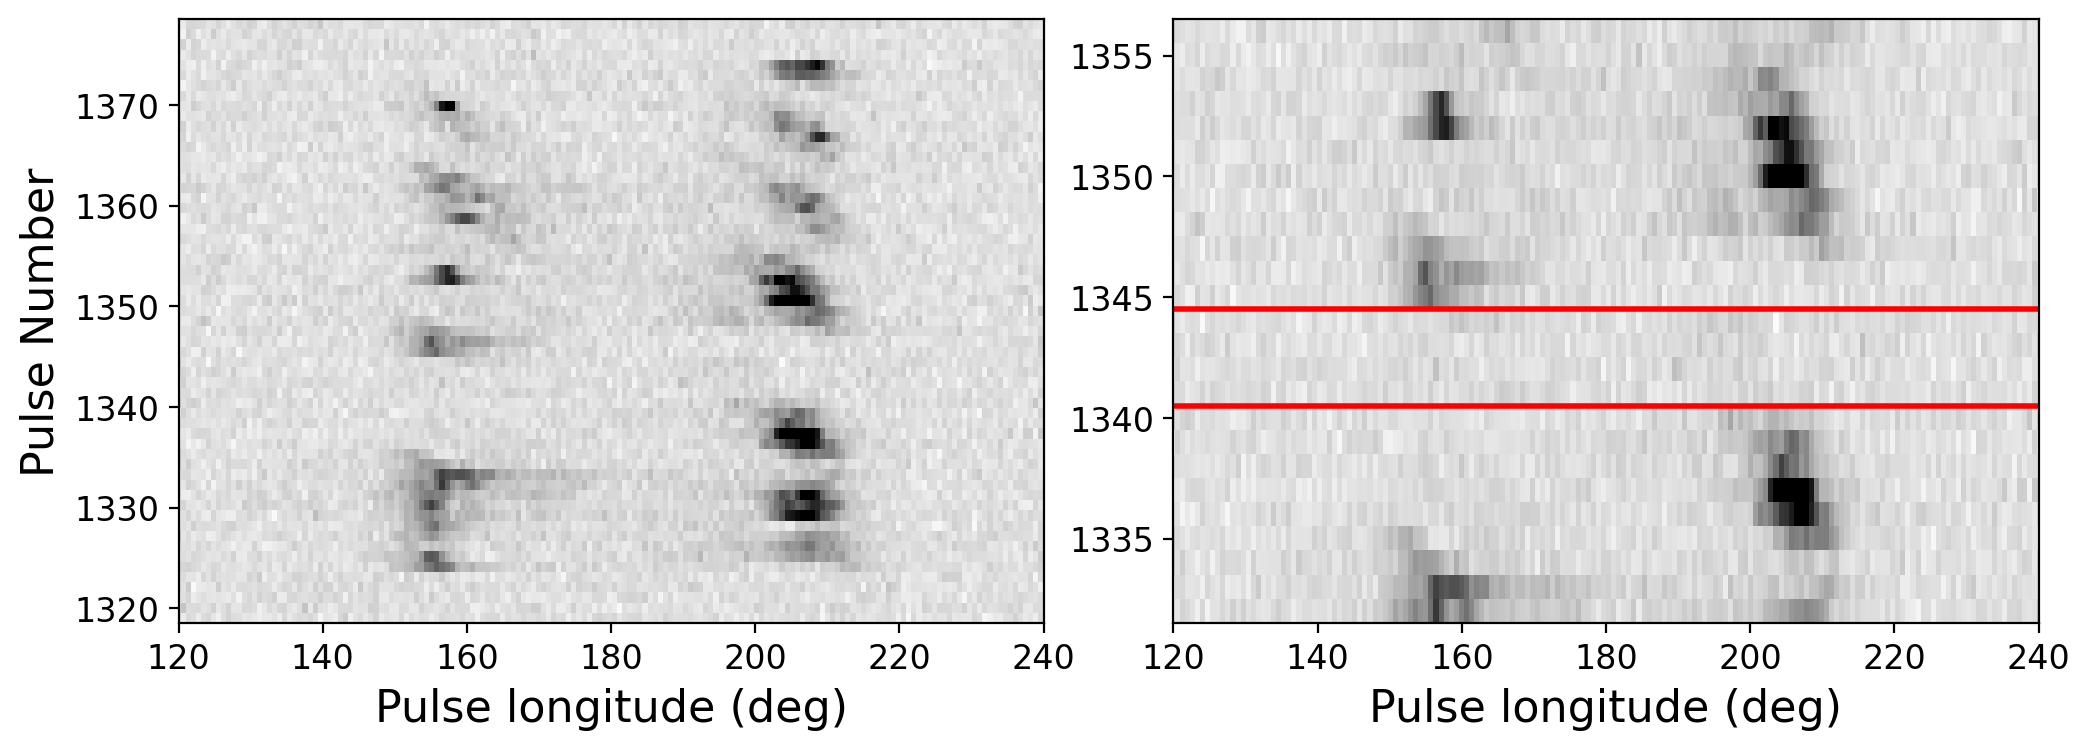
\includegraphics[width=1.0\textwidth]{Figures/J1926/burst_5}
        \caption[Burst 5 of PSR~J1926$-$0652 showing the possible null]{The single pulses observed with FAST, showing burst five. The red lines in the right-hand panel enclose those pulses for which no emission was detected in either component. It is unclear whether this is an example of a short null, or if this feature is due to the erratic drifting behaviour observed in this and the other short bursts.}
        \label{fig: J1926 - burst five null}
    \end{center}
\end{figure}
For these four rotations no emission integrated over the nominal pulse width is detected (following the method of \citet{BGGx2010} to identify single pulses), nor is the emission detected when the four are summed.
However, given the separation between the driftbands $P_3 \simeq 13P_1$, which moreover is clearly variable, it is  difficult to say for sure whether this is a true null or is simply part of the erratic drifting subpulse pattern as seen in the shorter bursts (see bursts 2, 4, 5, and 6 in Fig~\ref{fig: J1926 - pulse stack}).

As is the case for the potential null shown in Fig.~\ref{fig: J1926 - burst five null} and most of the clearer nulls, the leading half of the profile appears to disappear first. The `last active pulses' (LAPs) in the pulse stack before a null are shown in Fig~\ref{fig: J1926 - LAP and FAP profiles}. The `first active pulses' (FAPs) after a null are also shown. 
\begin{figure}
    \begin{center}
        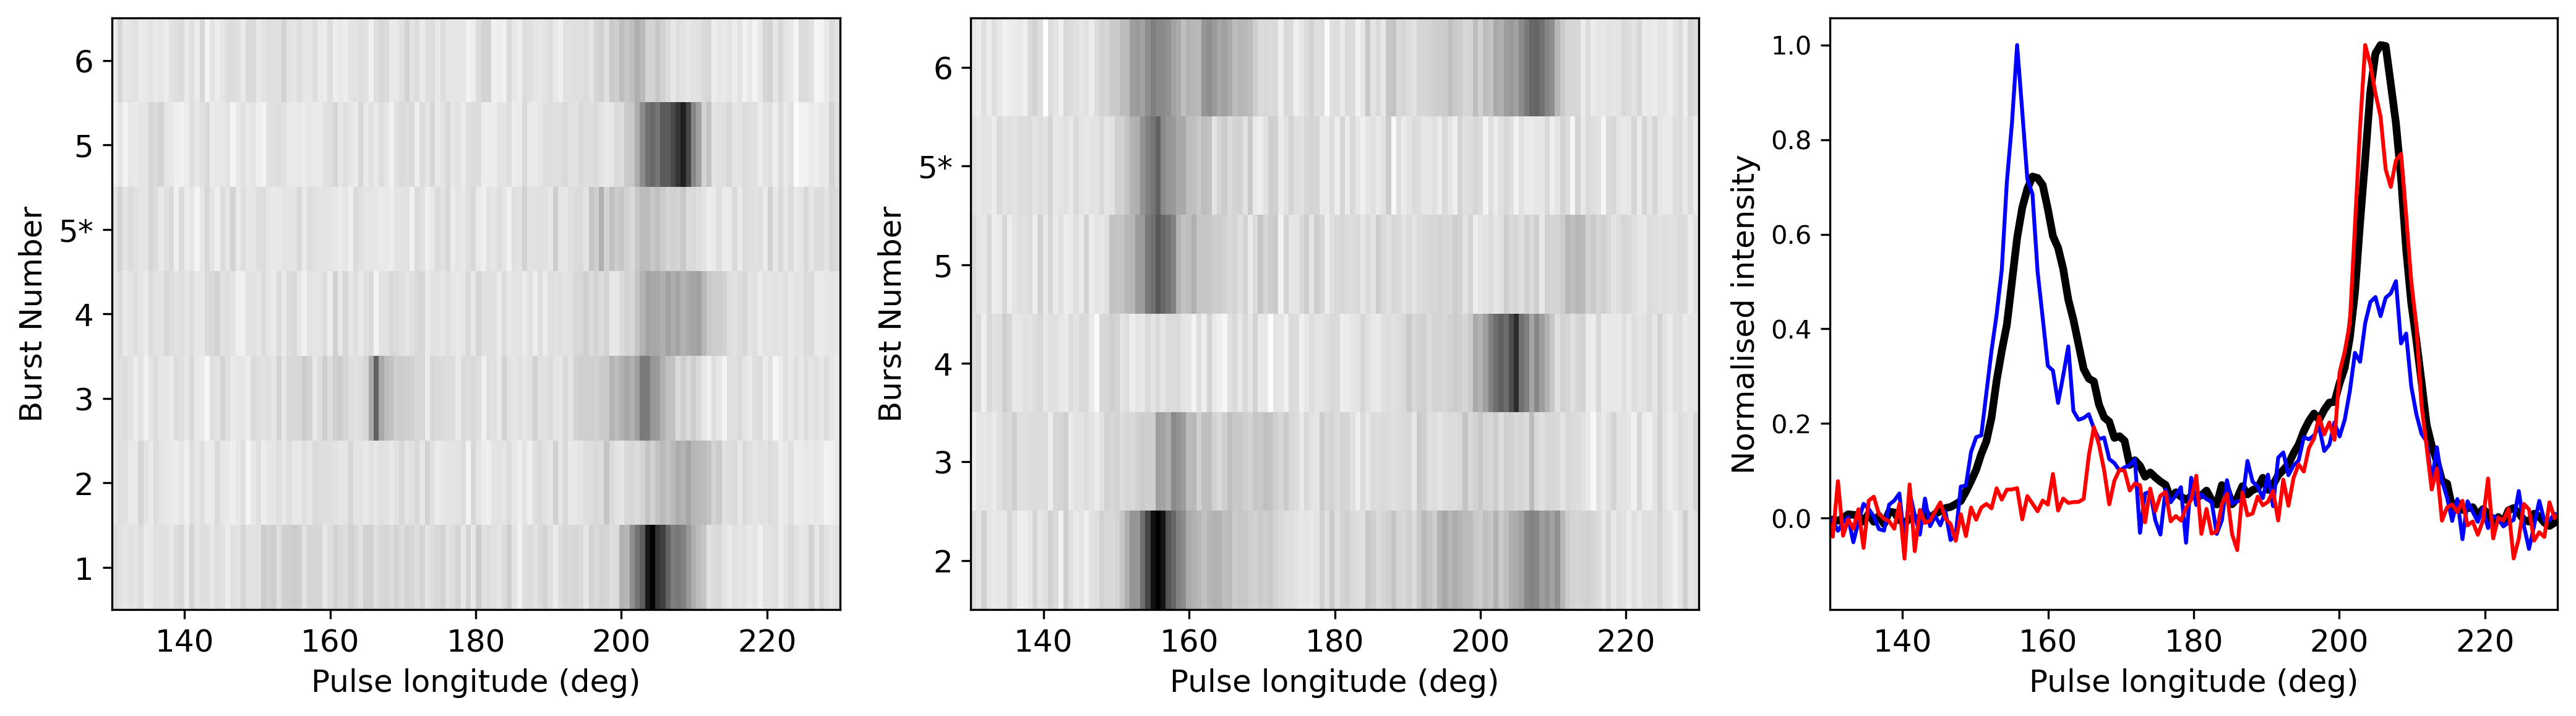
\includegraphics[width=1.0\textwidth]{Figures/J1926/LAPFAP_profiles}
        \caption[Comparison of LAP and FAP profiles to integrated profile]{The intensities of the individual LAPs (left panel) and FAPs (centre panel). The pulses for the bursts labelled `5*' correspond to the potential null in burst 5. The right-hand panel shows a comparison of the integrated profile of the full pulse stack (black line) to the integrated profiles of the LAPs (red) and the FAPs (blue). The profiles have been normalised to their respective peak intensities. }
        \label{fig: J1926 - LAP and FAP profiles}
    \end{center}
\end{figure}
There are seven LAPs shown in the left-hand panel, corresponding to the last pulses of bursts 1--6, and also including the potential short null in burst 5 which is labelled as burst 5*. There are only six FAPs however -- this is because at the start of the FAST observation PSR~J1926$-$0652 was already in its `on' state, so the FAP of burst 1 was not recorded. The LAPs and FAPs were summed to create an integrated profile for each set. These are shown in the right-hand panel of Fig.~\ref{fig: J1926 - LAP and FAP profiles} alongside the integrated profile for the entire pulse stack for comparison (thick black line). The LAP and FAP profiles are shown by the thinner red line and blue curves respectively.

The individual LAP pulses and their profile show very clearly that the leading components of the profile are distinctly weaker just before the pulsar enters the null state. The ratio between the leading and trailing profile components is extreme, far greater than in the overall average profile. A difference is also seen in the FAP profile, although the difference compared to the overall pulse profile is less extreme. The disappearance of the leading components immediately prior to a null suggests a link between the phenomenon of nulling and drifting subpulses. If the drifting subpulses are produced by sub-beams arranged in a circulating carousel pattern (see Chapter~\ref{chapt: B0031}), that would require the sub-beams to extinguish in a very specific sequence related to their circulation. This is discussed further in Sec.~\ref{sec: J1926 - discuss - LAP}.

Very few bursts of emission were observed by FAST, and the pulse shapes are highly variable, meaning that the difference between the LAP, FAP, and overall pulse profile might not be significant. The question we considered is `if the pulsar enters and leaves a null state at a random time (i.e. a random phase in the $P_3$ cycle), how likely is it to observe a LAP/FAP profile constructed from a few pulses which is as extreme as what is observed?'.
To quantify this, seven and six pulses (which corresponds to the number of LAP and FAP pulses respectively) were selected at random from all `on' state pulses (excluding the actual LAP and FAP pulses), and summed to create an integrated profile. From this profile the strengths of the leading and trailing profile components were calculated by integrating the flux density in their respective peaks, and their ratio $R$ was computed. This process was repeated 500,000 times. The results are shown in Fig.~\ref{fig: J1926 - LAP and FAP histograms}.


This ratio as determined from the observed LAP and FAP profiles (red and blue curves respectively in the right-hand panel of Fig.~\ref{fig: J1926 - LAP and FAP profiles}) is $R=0.154$ and $1.302$ respectively.  For comparison, the ratio in the integrated profile for the full pulse stack is $R = 0.896$.
\begin{figure}
    \begin{center}
        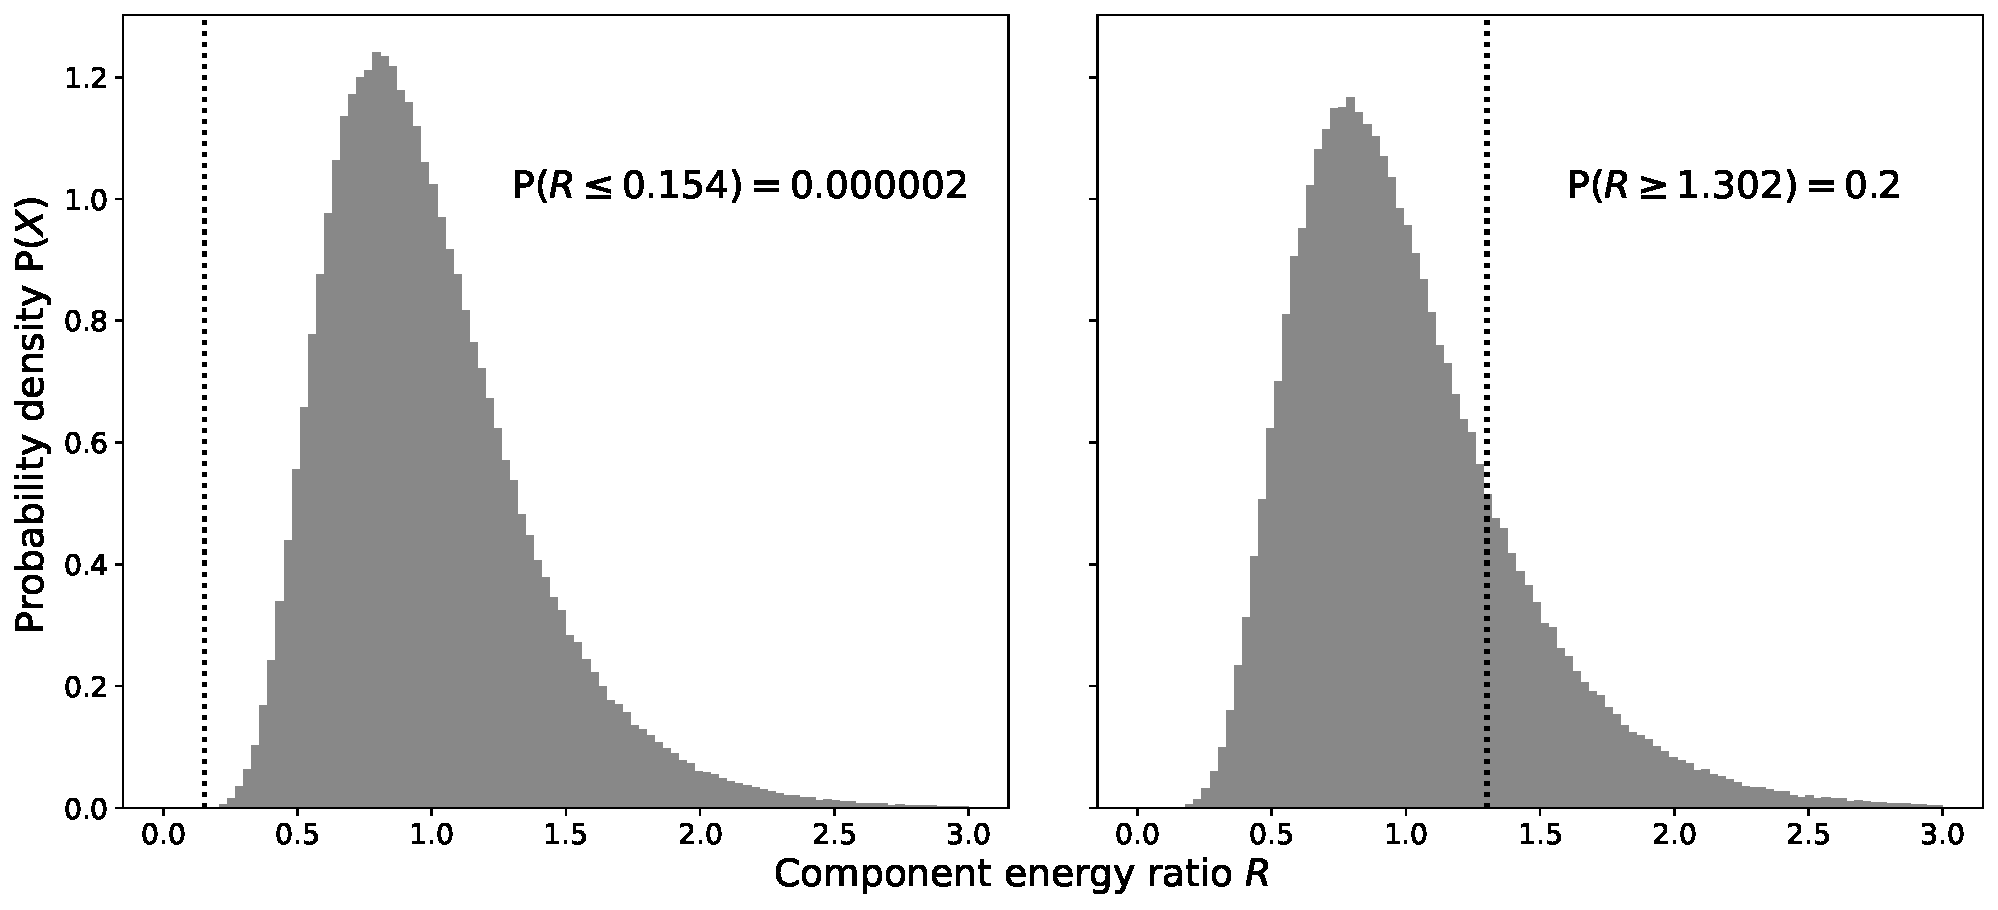
\includegraphics[width=1.0\textwidth]{Figures/J1926/LAPFAP_histograms}
        \caption[Calculating the significance of the LAP and FAP profiles]{Histograms showing the distribution of the peak power ratio of 500,000 randomly created integrated profiles corresponding to the LAPs (left panel) and FAPs (right panel). The vertical dashed lines indicate the measured ratio of the real integrated LAP (left) and FAP (right) profiles.}
        \label{fig: J1926 - LAP and FAP histograms}
    \end{center}
\end{figure}
Of the 500,000 trials, only one resulted in $R$ more extreme than that measured for the actual LAP profile. Therefore this difference between the LAP profiles and the overall profile is highly significant. In contrast, 99,980 randomised FAP profiles (20~per~cent) had a ratio $R$ greater than the observed FAP profile, so this is not significant given the low number of nulls recorded.

The analysis presented in this section is identical to that published in \citet{ZLH+2019}. In both cases, it was assumed that the four off-state pulses in burst 5 (Fig.~\ref{fig: J1926 - burst five null}) should be considered to be a null. If this is \textit{not} the case, $R$ would be 0.176 for the LAP profiles and the probability for this to occur at random would be $P(R\geq 0.176) = 0.003$, making the LAP profile still a $3\sigma$ outlier. We have therefore shown that there is a connection between the drifting subpulses and the time at which PSR~J1926$-$0652 enters a null, which will be discussed further in Sec.~\ref{sec: J1926 - discuss - LAP}.



















\section{Discussion}
\label{sec: J1926 - discussion}

PSR~J1926$-$0652 was one of the first new pulsars discovered by FAST, initially referred to fondly as `C12' (pulsar candidate 12). To date, FAST has found over 300 new pulsars, including 125 found during the Commensal Radio Astronomy FAST Survey\footnote{\url{https://crafts.bao.ac.cn/pulsar/}} \citep[CRAFTS;][]{LWQ+2018}, and a further 200 in the Galactic Plane Pulsar Snapshot (GPPS) survey \citep{HWW+2021}. Coming shortly after the publication of the first discovered pulsar \citep{QPL+2019}, the work on PSR~J1926$-$0652 by \citet{ZLH+2019} represents the first detailed investigation of the single pulse properties and polarisation of a pulsar found by FAST. This work therefore paves the way for future studies with this powerful telescope.

\subsection{Profile and geometry}
\label{sec: J1926 - discuss - geometry}

The integrated pulse profile of PSR~J1926$-$0652 has four components: two bright, primary components (C1 and C4); and two somewhat dimmer, inner components (C2 and C3). There is also a bridge of weak emission connecting the leading and trailing halves. The overall structure is a twin-peaked profile. Various models of the emission region have been put forward to explain the variety of profile shapes found across the population (see \citealt{KJxx2007} for a full review and empirical model) -- these include the core-cone model \citep[e.g.][]{Rxxx1983a, Rxxx1986}, and the `patchy beam' of \citet{LMxx1988}. This work does not explicitly rule out any beam model; however, the fact that drifting subpulses are observed in the leading and trailing components means that it is likely that this profile shape arises from the line of sight intercepting a ring of circulating sub-beams arranged in a carousel structure. This is further discussed in Sec.~\ref{sec: J1926 - discuss - phase track}.

The profile becomes narrower with increasing frequency, as demonstrated by Fig.~\ref{fig: J1926 - p3 folds}. This is a commonly observed phenomenon \citep[e.g.][]{CWxx2014,PHS+2016}, and is the expected behaviour if the higher frequencies are produced at lower altitudes in the magnetosphere, where the open-field-line region is narrower \citep[e.g.][]{RSxx1975,KGxx2003}. In Fig.~\ref{fig: J1926 - p3 folds} it appears as though the narrowing of the profile is caused by the movement of the leading profile components to later pulse longitudes while the trailing component remains at a constant phase. However, this behaviour depends on the choice one makes for the dispersion measure (DM; see Sec.~\ref{sec: intro - observation processing - ISM effects - dispersion}). The measured DM for PSR~J1926$-$0652 is $84.7 \pm 0.9\ \mathrm{cm}^{-3}\mathrm{pc}$ \citep{ZLH+2019}. This choice of DM follows from optimising the overall S/N of the integrated pulse profile. This optimisation will attempt to align the pulse profile as a function of frequency after removal of the frequency-dependent dispersive delay. However, if the profile itself is frequency-dependent, it is difficult to disentangle the two contributions. This is illustrated in Fig.~\ref{fig: J1926 - dedispersion}.
% \begin{figure}
%     \begin{center}
%         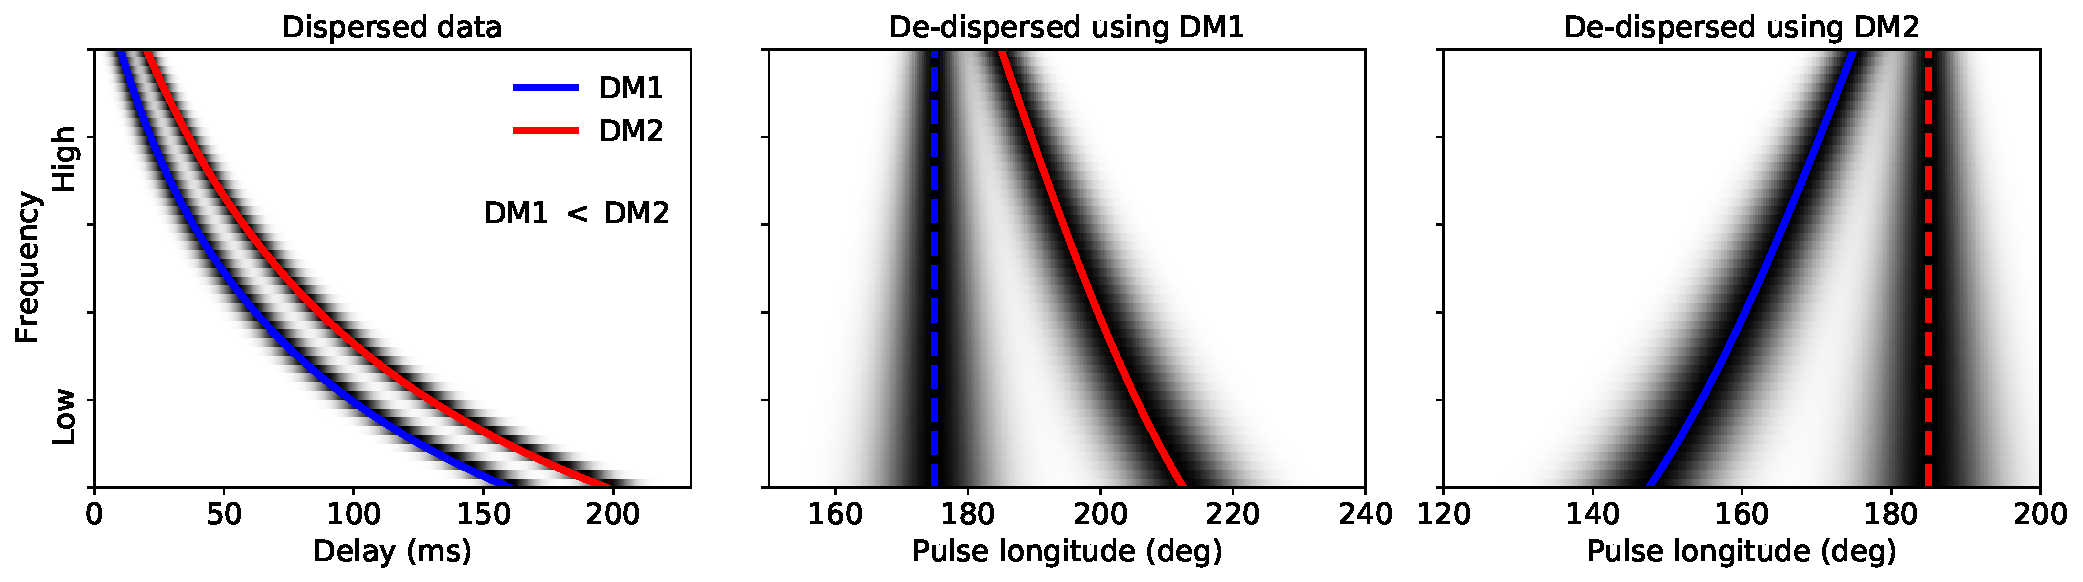
\includegraphics[width=1.0\textwidth]{Figures/J1926/dedispersion_demo}
%         \caption[Ambiguity in de-dispersion of a multi-component pulse profile]{An illustration of the ambiguity encountered when de-dispersing data for a pulsar with a twin-peaked profile. The components of the profile move closer together at higher frequencies, meaning that two slightly different DMs may be measured in the frequency-resolved dispersed data (left panel). The blue and red lines correspond to the peak of each component as a function of frequency. Due to the changing position of the components a DM optimising the S/N of the earlier component (DM1) will be slightly smaller than the DM optimising the S/N of the trailing component (DM2). De-dispersing using DM1 will lead to the leading component remaining stationary in pulse phase while the trailing component appears to shift to earlier longitudes at higher frequencies (centre panel), while de-dispersion using DM2 will lead to the opposite (right panel).}
%         \label{fig: J1926 - dedispersion}
%     \end{center}
% \end{figure}
\begin{figure}
    \begin{center}
        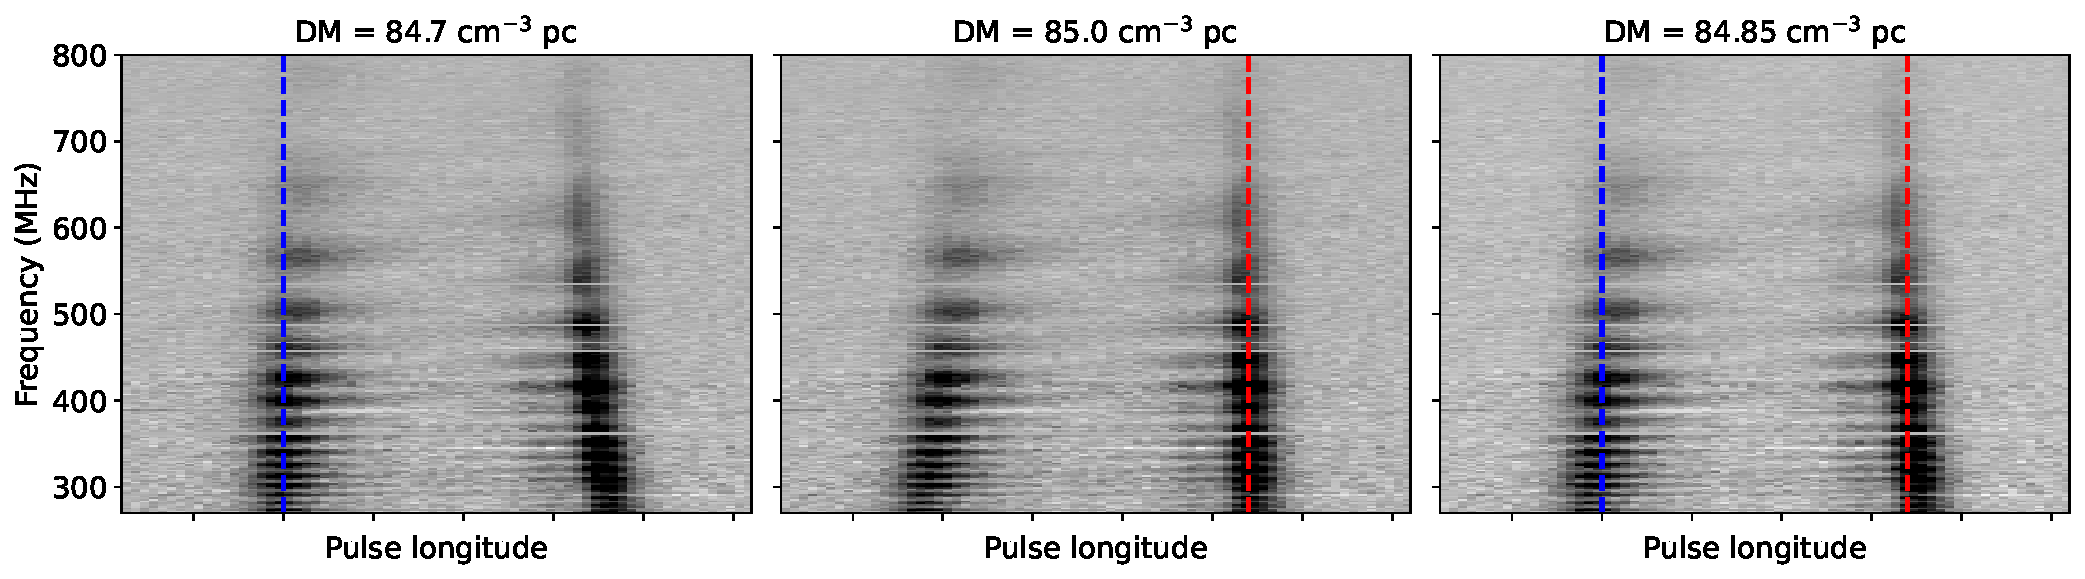
\includegraphics[width=1.0\textwidth]{Figures/J1926/dedispersion_real_data}
        \caption[Ambiguity in de-dispersion of a multi-component pulse profile]{An illustration of the ambiguity encountered when de-dispersing the twin-peaked profile of PSR~J1926$-$0652, where the profile components move closer together at higher frequencies. The left-hand panel shows the data de-dispersed using DM$=84.7$~cm$^{-3}$~pc, which maximises the S/N of the leading component and causes the trailing component to move to earlier pulse longitudes at higher frequencies. The centre panel shows the result of using  DM$=85.0$~cm$^{-3}$~pc, which maximises the S/N of the trailing component and the leading component now moves. De-dispersing using an intermediate value of DM$=84.85$~cm$^{-3}$~pc will lead to both components moving together simultaneously as frequency increases (right-hand panel). All three of these values lie within the uncertainty of the measured DM of $84.7 \pm 0.9$~cm$^{-3}$~pc, which was fitted by maximising the S/N of the profile as a whole \citep{ZLH+2019}. Note: the apparent periodicity in intensity as a function of frequency in both profile components is due to Faraday rotation (see Sec.~\ref{sec: intro - observation processing - ISM effects - faraday rotation}) since only one linear polarisation path of FAST was used.}
        \label{fig: J1926 - dedispersion}
    \end{center}
\end{figure}
De-dispersing with different DMs may either align one or the other component across the frequency band, whilst the other appears to change pulse longitude. It is likely that the profile of PSR~J1926$-$0652 narrows uniformly with increasing frequency, which would mean both components move inwards rather than one component being stationary.

The Parkes telescope data of PSR~J1926$-$0652 shows that its PA curve is fitted very well by the RVM (see Fig.~\ref{fig: J1926 - parkes profile}). Despite the excellent fit, the magnetic inclination angle $\alpha$ remained unconstrained. Further constraints were applied based on the observed profile width, which is reasonably broad spanning $\sim$60$\degr$ pulse longitude, suggesting that $\alpha \lesssim 55\degr$. A broad profile can occur in two ways: if the emission is produced at high altitudes, in which case the emission cone formed by the tangents to the last open field lines will be very wide; or if $\alpha$ is small in which case the observer's line of sight can spend longer within the emission beam as the pulsar rotates. An upper limit was placed on the emission height by measuring the delay between the fiducial plane of the total intensity profile and the inflection point of the PA curve due to relativistic aberration and retardation effects \citep{BCWx1991}. The upper limit was estimated to be $14\degr$, which is large in order to account for the uncertainty in the location of the fiducial plane. Given the double-peaked nature and drifting subpulses with the same periodicity detected in both, the beam is likely to be conal \citep{Rxxx1983a} with the fiducial plane being somewhere between the two peaks. This corresponds to an upper limit on the emission height of $\sim$5000~km. The emission height of most radio pulsars is believed to be less than 1000~km \citep[e.g.][]{KJxx2007,JKxx2019,JSKx2020} so somewhat lower than the estimated upper limit for PSR~J1926$-$0652: taking this to be the emission altitude would shrink the constraints on the magnetic inclination angle, giving $\alpha \lesssim 21\degr$. The conclusion that remains is that this pulsar is moderately aligned.






\subsection{Drifting properties and subpulse phase track}
\label{sec: J1926 - discuss - phase track}


PSR~J1926$-$0652 exhibits well-defined drifting subpulses, with an average periodicity of $P_3 = (17.4 \pm 0.1) P_1$. The drifting subpulses are stable in the longest bursts, but in the shorter bursts the driftband shapes and their separation are much more erratic, with large variations in $P_3$. For example, the average separation of successive bands in burst 5 is approximately seven periods, less than half the average for the full pulse stack -- in the framework of the carousel model this could point towards a shorter circulation period ($P_4$), but coupled with the instability in the subpulse shape could equally be due to fragmentation of the sub-beams.

The drifting subpulses are seen in both profile peaks, but not in the central bridge region. This indicates that the line of sight probes a region in the middle of the carousel of rotating sub-beams which contains much weaker emission. Some faint periodic emission was observed for the inner components C2 and C3. The longest burst, burst 3, was $P_3$-folded to detect this weak emission more clearly (Fig.~\ref{fig: J1926 - p3 folds}), and frequency-resolved subpulse phase tracks (Fig.~\ref{fig: J1926 - phase tracks}) were also calculated for this burst and burst 1 to further highlight the structure of the drifting subpulse pattern. In the framework of the carousel model the four profile components can be interpreted as originating from two nested, phase-locked (i.e. sharing a common circulation period) carousels, each containing the same number of sparks (in order to exhibit the same $P_3$). Such a model has previously been used to explain the drifting subpulses of PSR~B0808$-$41 \citep{BBGx2009}.  

The subpulse phase tracks reveal a kink in the trailing half of the profile, between components C3 and C4. This kink is present in both burst 1 and burst 3, shown in the left- and right-hand panels of Fig.~\ref{fig: J1926 - phase tracks} respectively. The kink shows no significant variation with frequency in either burst, however at low frequencies a kink begins to appear in the leading half as well, being more pronounced in burst 3. Inspecting the fluctuation spectra of PSR~J1926$-$0652, a notch can be seen in the longitude-resolved modulation index, shown in the upper left panel of Fig.~\ref{fig: J1926 - fluctuation spectra}. This notch aligns with the kink in the trailing half of the subpulse phase track. It was argued by \citet{ESLx2003} that interference between superposed, out-of-phase drifting subpulse signals would result in a localised decrease in the modulation index, accompanied by a rapid swing in the subpulse phase angle. Again, this is consistent with the idea of nested carousels.  

The asymmetry of the subpulse phase tracks and $P_3$-fold would be problematic for a naive application of the carousel model; however, as demonstrated in Chapter~\ref{chapt: B0031} this can be resolved if longitude-dependent polarisation effects are allowed to occur. The single pulses of PSR~J1926$-$0652 recorded with FAST only consist of one linear polarisation path, which means that their polarisation properties are unknown -- orthogonal polarisation mode (OPM) transitions such as those seen in PSR~B0031$-$07 could account for the kinks in the subpulse phase track. On the other hand, a single OPM is likely to dominate at all pulse longitudes at 1.4~GHz, since the polarisation as observed by Parkes is shown to be fitted well by the RVM.

The instability of $P_3$ in the shorter bursts and the variable driftband shapes does not fit naturally with the carousel model, however. Other models for drifting subpulses do exist -- for example, \citet{GMML2005} proposed a purely magnetospheric model (not related to processes in the polar cap) based on long wavelength drift waves. The electric fields of standing waves are directed along the magnetic field lines, modulating the plasma distribution and hence the radio emission mechanism. The predicted observations of this are similar to the model of non-radial oscillations of the neutron star \citep[e.g.][]{DCxx1968, CRxx2004}, which can account for discontinuous features such as subpulse phase steps. These have been observed in a number of pulsars, including PSRs~B0320+39 and B0809+74 \citep{ESLx2003,ESxx2003b}, and PSR~B1919+21 \citep{PWxx1986,WSEx2007}. The frequency evolution of the kink in the leading half of the subpulse phase track of PSR~J1926$-$0652 may tentatively point to such a feature, similar to that seen in PSR~B0809+74 \citep{HSW+2013}.

Overall, PSR~J1926$-$0652 exhibits complex drifting behaviour across four profile components, which is not inconsistent with emission from two nested, phase-locked carousels.  However, the value of $P_3$ is stable in the longer bursts but more erratic in shorter ones, which casts some doubt on this. This could be indicative of a more turbulent, unstable magnetosphere at these times, leading to rapid changes between emission states that may be linked to this pulsar's high nulling fraction.



\subsection{Nulling and the last active pulse phenomenon}
\label{sec: J1926 - discuss - LAP}

The nulling behaviour in PSR~J1926$-$0652 is more than simply the disappearance of its radio emission. The leading half of the profile is significantly weaker than the trailing half in the last active pulse before a null, with the observed flux density ratio between the two components being extremely unlikely to have occurred at random. 
There are two alternative scenarios to consider. First of all, the leading half of the profile could fade slowly over several periods during which the periodic modulation continues as normal, entering the null state before the trailing components. Alternatively, the timing of the nulls are organised in such a way that they occur when at a minimum in the modulation cycle of the leading half of the profile.

As a requirement for the second scenario to be possible, it should be the case that the leading components become sufficiently weak in between driftbands in the normal, `on' state. This was tested by calculating the profile power ratio for all individual pulses, using a similar method to that used to test the significance of the different shape of the LAPs. In about 4~per~cent of the individual `on' state pulses the ratio is at least as extreme compared to what is observed for the integrated LAP profile, and in a further 4~percent the leading component is detected with a significance of $3\sigma$ or less. So a scenario in which the nulls are coordinated with the drifting subpulses such that they happen at the weakest part of the modulation cycle in the leading components is at least a mechanism that should be considered.

There is an observational precedence for such an effect. \citet{GYY+2017} studied PSRs~J1741$-$0840 and J1840$-$0840, both nulling pulsars with a nulling fraction between 30 to 50~per~cent, and both have drifting subpulses. Like PSR~J1926$-$0652, both these pulsars display distinct twin-component profiles. 
Following the suggestions of \citet{JVxx2000}, \citet{GYY+2017} measured the pulse longitudes at which the profile components switch off and switch on, as a proxy for subpulse phase. 
It was found that both components transition simultaneously, but in such a way that PSR~J1840$-$0840 showed a very strong preference for the nulls to start after completion of a full driftband, and have a high probability of finishing at the start of a new driftband in either component. This also implies that the typical length of a burst in this pulsar are integer multiples of $P_3/P_1$ pulses.

To test if the nulls of PSR~J1926$-$0652 tend to start at a minimum in the modulation cycle, the phase in the modulation cycle was estimated by eye for each null. A Kolmogorov-Smirnov (KS) test showed that the resulting phase distribution is indistinguishable from a uniform distribution. However with only seven LAPs observed (compared to the 21 nulls observed by \citealt{GYY+2017} in PSR~J1840$-$0840) the absence of a significant correlation is not too surprising, especially given that the variable $P_3$ and narrow shape of the driftbands meant that the phase estimates have a large margin of error. So there is no evidence that nulls tend to happen during the weakest part of the modulation cycle in the leading profile components of PSR~J1926$-$0652, but neither can it be completely ruled out. Longer observations to produce a larger sample of null state transitions would be able to answer if nulls and drifting subpulses are related phenomena in this way. 

The `missing line of sight' model can only explain some aspects of the link between nulling and drifting subpulses. If a sub-beam within a carousel is extinguished, no emission would be observable when the line of sight passes over it. This would lead to null states with an underlying periodicity \citep{HRxx2007, HRxx2009}, and nulls occurring at a minimum in the $P_3$ cycle. This model can also explain a number of pulsars which exhibit partial nulling, i.e. nulls occurring in only one profile component \citep{LAxx1983, Vxxx1995,LKR+2002,JLxx2004}. However the profile components in both PSRs~J1840$-$0840 and J1926$-$0652 transition to and from a null state simultaneously, whereas the missing line of sight model would predict that for clear double-peaked profiles the null state happens at different times in the two components. Note that although the apparent null in burst 5 (Fig.~\ref{fig: J1926 - burst five null}) could be an example of a null state beginning and ending at different times in the two profile components, it would not be possible to explain this by a missing sub-beam. Since the subpulses drift towards the leading edge of the profile, the null should start and end in the trailing half of the profile first. This is the opposite to what is observed.

The alternative to nulls being linked to the modulation cycle is a scenario in which the leading component starts fading earlier, and fades away slower than the trailing component. This resembles PSR~B1944+17, for which \citet{DCHR1986} found that nulls are preceded by a decay in intensity of approximately 50~per~cent over the course of about three pulse periods. In addition, they found that the last active pulses were quantitatively different in shape and more variable compared to other pulses. \citet{DCHR1986} argue that the slow decay observed in PSR~B1944+17 may be explained by the model of \citet{FRxx1982}. In this framework a transition to the null state is due to a change from a state of rapid spark discharges (producing bunches of charged particles that emit coherently) to a steady discharge, which no longer produces coherent emission. The potential drop slowly decreases during the transition to the steady discharge state, and this might explain the intensity decay seen before a null in PSR~B1944+17.

A second example of a pulsar with a decay in intensity before the start of a null is PSR~J1727$-$2739 \citep{WWY+2016}, where transitions occur both rapidly and more gradually. In addition, an abrupt rise in intensity after a null lasting around six pulse periods is observed. Like PSR~J1926$-$0652, J1727$-$2739 has a twin-peaked profile and the leading component in the LAPs is dimmer (although this effect is far more pronounced in PSR~J1926$-$0652). In addition (and in contrast to PSR~J1926$-$0652) it shows a different profile shape for the first active pulses (FAPs) after a null, this time with the trailing component being dimmer \citep{WWY+2016}. The slow decay and recovery of the emission implies larger, global magnetospheric transition are taking place \citep{LHK+2010,MYxx2014} with the gradual decay to a null indicative of a steady relaxation. \citet{WMJx2007} suggested that emission can turn on or off rapidly if the magnetic or charge configuration reaches a critical state, although the trigger for such a state change is yet to be determined.

The curious behaviour observed in PSR~J1926$-$0652 adds to the miscellany of interesting findings surrounding drifting and nulling, and strengthens the arguments that the two are intimately related. It is clear that further observations of this and other similar pulsars are needed, as there is currently no model which can satisfactorily explain these phenomena.




\section{Summary and conclusions}
\label{sec: J1926 - conclusions}


PSR~J1926$-$0652 is a newly discovered pulsar that displays a variety of interesting phenomena, predominantly in its single pulses as observed between 270 to 800~MHz with FAST during commissioning. These phenomena include drifting subpulses and nulling, with six bursts of emission observed by FAST. Polarisation information was provided by a long-term timing programme performed using Parkes at 1400~MHz.

The pulsar has a twin-peaked profile with two weaker components nested on the inner edge of the stronger main components, falling into the `conal-double' morphology classification \citep{Rxxx1983a}. 
The overall profile shape shows little frequency evolution, and is comparable in the FAST and Parkes observations. It becomes slightly broader at lower frequencies, which is consistent with the expectations from radius-to-frequency mapping \citep[e.g.][]{Cxxx1978}. When the `optimum' dispersion measure (DM) is used, it appears that in the FAST data the leading component moves to later pulse longitudes at lower frequencies whilst the trailing component appears stationary. However, it was demonstrated that this could equally well be an overall broadening of the profile within the uncertainty arising from the degeneracy in the measurement of the DM for a profile with intrinsic frequency evolution.

Polarisation data recorded with Parkes show that (at least at 1400~MHz) the PA as a function of pulse longitude follows the canonical S-shaped RVM remarkably well. Fitting the RVM to these data shows that the impact parameter of the observer's line of sight $|\beta| < 14\degr$, however the magnetic inclination angle $\alpha$ is unconstrained by the polarisation properties alone. The observed profile width of $\sim$60$\degr$ was used to further constrain $\alpha \lesssim 55\degr$ by measuring aberration and retardation effects, or $\alpha \lesssim 13\degr$ assuming a low emission height consistent with the rest of the non-recycled population \citep{JKxx2019}, making it a moderately aligned rotator.

Drifting subpulses are present in all six bursts in the single pulse data, with an average $P_3 = (17.4\pm 0.1) P_1$. The driftbands are most clear under the main profile peaks (components C1 and C4), with fainter driftbands appearing under components C2 and C3. No significant single pulse modulation was observed in the faint bridge of emission between the peaks. This is consistent with the pattern that would be observed from a pair of nested, phase-locked carousels. The drifting is most stable in the longer busts (bursts 1 and 3), becoming much more variable in the shorter bursts, and changes in the shape of the driftbands were also observed. 
The driftbands at the end of burst 3 appear to move to slightly later longitudes (see Fig.~\ref{fig: J1926 - pulse stack}) and start to become less stable, which may be connected to the more erratic, shorter successive bursts.
It was revealed by $P_3$-folding that the drifting subpulses in component C3 appear to be out of phase with the modulated emission of component C4. Subpulse phase tracks were created for this burst and burst 1, and show that in both there is a distinct kink in the phase as a function of pulse longitude at the intersection between C3 and C4. A similar, albeit less extreme kink, between components C1 and C2 is visible at lower frequencies. These features are consistent with nested carousels if their sub-beams are out of phase. The asymmetry of the driftband shapes could potentially be explained if the magnetospheric mixing model of Chapter~\ref{chapt: B0031} can be applied, but this would require single pulse observations with full polarisation information to be confirmed.

Before a null starts the leading half of the profile becomes significantly dimmer. A similar effect has been observed in a few other pulsars, but is absent for most that show nulling. It was calculated that such an extreme flux density ratio between the two halves of the profile before the nulls start has a one in 500,000 chance of occurring at random. This high significance is despite the low number of transitions observed for PSR~J1926$-$0652, and reflects how strong the observed effect is for this pulsar. No evidence was found for the emission after a null being different compared to typical pulses observed during the active phase of the pulsar. The full null state occurs simultaneously in both profile halves: this rules out a model for the nulls being caused by one or more sparks extinguishing in a circulating carousel \citep[e.g.][]{RWxx2008}. Instead a global magnetospheric change appears responsible, which is something mode changes and nulling have in common.

In conclusion, PSR~J1926$-$0652 is a fascinating pulsar whose single pulse properties cannot be adequately explained by existing models. Further observations with the now fully operational FAST and other large radio telescopes are required to examine its behaviour in more detail, which will help to build a coherent picture of the connection between the drifting subpulse and nulling mechanisms. 
\chapter[FAST observations of an MSP]{Curious single-pulse modulation in the millisecond pulsar J1518+4904}
\label{chapt: J1518}

This chapter details observations of PSR~J1518+4904, a millisecond pulsar in a binary system which, along with PSRs J1012+5307 and J1713+0747, is one of three MSPs with known drifting subpulses. The observations were performed with FAST during its commissioning phase. These observations are part of a programme to exploit the sensitivity of the telescope to produce `technical test and science demonstration data' to allow the study of timing noise in pulsars. The observations revealed two previously unknown profile components that greatly extend the overall pulse width, and multiple distinct periodicities in the single pulse data which seem to happen simultaneously. It therefore cannot be attributed to mode-switching behaviour. In addition to the distinct periodicities, there also appears to be a smooth pulse longitude dependence of the fluctuation frequency across different pulse profile components, which cannot be explained with existing models of the production of radio emission in pulsars.

\section{Introduction}
\label{sec: J1518 - intro}

PSR~J1518+4904 is a millisecond binary pulsar with a period of 40.9~ms discovered in the Green Bank Northern Sky Survey \citep{NSTx1996,SNTx1997}. Its companion is a neutron star, making it one of at least 15 known double neutron star (DNS) systems \citep{TKF+2017}. PSR~J1518+4904 has a mean flux density of $2.5\pm2$~mJy at 1.4~GHz \citep{LKG+2016} and is a recycled pulsar. Recycled pulsars are older objects which accrete matter from their binary companions, transferring angular momentum to the pulsar and causing it to spin-up to a typical rotational speed of hundreds of rotations per second \citep[e.g.][]{PulsarAstronomy}. An overview of the pulsar population is given in Sec.~\ref{sec: intro - general intro - pulsar population}.% Recycled pulsars are objects which have at some point in the past undergone mass accretion from their binary companion; this causes them to spin-up to a typical rotational speed of hundreds of rotations per second \citep[e.g.][]{PulsarAstronomy}. Before spin-up these were older, normal pulsars, decaying in luminosity as they lose energy -- the increase in rotational energy through accretion rejuvenates them causing them to once again emit radio waves. An overview of the pulsar population is given in Sec.~\ref{sec: intro - general intro - pulsar population}.

Previous studies have found that PSR~J1518+4904 has a relatively narrow pulse profile compared to many other millisecond pulsars (MSPs), with a duty cycle $W_{10} = 5.4\pm0.2$~per~cent compared to an mean of $\langle W_{10} \rangle= 21$~per~cent across the MSP population  at 1.4~GHz \citep{KXL+1998}. The integrated profiles of MSPs are generally much wider than those of ordinary pulsars, and are often more complex with more components \citep[e.g.][]{YMS+2011}, although their spectral properties are similar \citep{TBMS1998, KXL+1998, KLL+1999}. By investigating and comparing the radio properties and $\gamma$-ray beaming of MSPs and normal pulsars, \citet{Mxxx2005} and \citet{RMHx2010} suggest that the radio emission of MSPs is produced at high altitudes within the magnetosphere (as a fraction of the light cylinder radius) -- possibly the `outer gap' which is usually associated with high-energy emission \citep[e.g.][]{CZxx1998} -- resulting in very wide beams. \citet{NSTx1996} studied PSR~J1518+4904 between 320 and 1400~MHz, and their data show a double-peaked profile with a stronger leading component, and a broad tail at the lower frequencies. This pulsar was part of a study of the properties of MSPs by \citet{KXL+1998} who discovered that the profile shows a postcursor at 1.4~GHz. The postcursor is separated from the centre of the main profile by approximately $25\degr$, but is connected to it by low-intensity emission. A subsequent multi-frequency study of the pulsar \citep{KLL+1999} showed that this postcursor disappears at higher frequencies, and also at lower frequencies because it becomes swamped by the tail of the main component \citep{NSTx1996,STCx1999}.


PSR~J1518+4904 was initially selected for observation by the Five-hundred-metre Aperture Spherical radio Telescope (FAST) during commissioning to test the telescope performance and capabilities, but also because it is a promising source to study `jitter noise'. Jitter noise is related to the fact that the individual pulses of pulsars are variable in shape (for example due to effects described in Sec.~\ref{sec: intro - emission models - single pulse phenomena}). This affects the precision with which arrival times can be measured, hence resulting in uncertainties in the timing precision of pulsars. This stochastic uncertainty comes on top of potentially correlated `red' timing noise which represents unmodeled variations in the spin-down of pulsars. The rapid rotation of MSPs means that typically large numbers of pulses are collected in a single observation, thereby averaging out much (but not all) of the jitter noise. The high precision in timing for a small selection of the MSP population makes them ideal probes to try to detect gravitational waves \citep[e.g.][]{FBxx1990,MHB+2013}, which affect pulse arrival times by very small amounts. A better understanding of timing noise can be crucial in order to achieve the highest possible timing precision, thus maximising the sensitivity for detecting gravitational waves. A large telescope such as FAST can provide the most sensitive arrival time measurements, and is ideal to study the pulse-to-pulse variations in the pulse shape of MSPs as their individual pulses can be detected with enough significance.


Quasi-periodic modulation was detected throughout the main profile component of PSR~J1518+4904 by \citet{ESxx2003} using 1650 single pulses from archival data at 1.4~GHz recorded using the Westerbork Synthesis Radio Telescope (WSRT). Using a two-dimensional fluctuation spectrum (2DFS, as described in Sec.~\ref{sec: J1926 - analysis - single pulse variability}), they detected modulation with frequency $P_3\sim0.38$~cpp and $P_2\sim 10$~cpp (see Sec.~\ref{sec: intro - emission models - single pulse phenomena} for the definition of $P_2$ and $P_3$). 
A motivation for developing the 2DFS by \citet{ESxx2002} was to be able to detect periodic pulse shape variations even when the pulsar signal is not strong enough to detect the individual pulses with high significance, making the results of \citet{ESxx2003} especially satisfying. The positive value of $P_2$ demonstrates that PSR~J1518+4904 has drifting subpulses that move rapidly from earlier longitudes to later longitudes across the pulse profile\footnote{In the original paper $P_2$ was quoted as negative -- this is due to a different convention in the sign. In this thesis, a positive $P_2$ corresponds to drift towards later longitudes.}. This finding, along with similar behaviour in PSR~J1012+5307, was the first ever detection of drifting subpulses in recycled pulsars \citep{ESxx2003}, suggesting that the magnetospheric physics might be very similar in MSPs and slower pulsars, despite their vastly different light-cylinder radii (see Sec.~\ref{sec: intro - general intro - pulsar population}). This knowledge led us to propose additional observations of PSR~J1518+4904 to be performed with FAST after the existing observation aimed at studying the jitter noise, in order to study this modulation behaviour in unprecedented detail.

Drifting subpulses were later discovered in another MSP, PSR~J1713+0747 \citep{LBJ+2016}. This finding increases the known number of MSP drifters to three -- however, given that high-sensitivity searches for drifting subpulses have been performed for only approximately ten MSPs, the phenomenon does not appear to be unusual, and is comparable to what is found for the non-recycled pulsar population \citep[more than 55~per~cent;][]{WESx2007}. All three MSPs are classified as `diffuse' drifters by the definition of \citet{WESx2006}. These are pulsars which have a vertically broad $P_3$ feature in their spectra, in contrast with `coherent' drifters which have well-defined, narrow $P_3$ features that indicate that the periodicity of the pulse-to-pulse modulation is stable throughout the observation. In a sample of 192 (mostly non-recycled) pulsars \citep[Table 2]{WESx2006} 21 were identified as coherent drifters and 51 as diffuse drifters, meaning that unstable $P_3$ appears to be commonplace. 

This chapter is structured as follows. In Sec.~\ref{sec: J1518 - observations} the observations are summarised, along with the properties of the processed data that were available for analysis. In Sec.~\ref{sec: J1518 - analysis - new profile component} we present the discovery of two new profile components. In Sec.~\ref{sec: J1518 - analysis - LRFS} and Sec.~\ref{sec: J1518 - analysis - 2DFS} we investigate the single-pulse modulation and drifting behaviour, and show that there are at least two distinct periodicities present. In Sec.~\ref{sec: J1518 - analysis - drifting P3} we highlight that in the main part of the profile the periodicity appears to be pulse longitude-dependent. We show in Sec.~\ref{sec: J1518 - analysis - disjoint modes} that there is no evidence that these are the result of distinct switches such that only one periodicity is present at a given time. We also explore the longitude-resolved auto- and cross-correlation functions to highlight this longitude-dependent periodicity further in Sec.~\ref{sec: J1518 - analysis - correlation}. We discuss the implications of the extra profile components and highlight the complications in explaining the observed drifting subpulses with current theory in Sec.~\ref{sec: J1518 - discussion}.


\section{Summary of observations}
\label{sec: J1518 - observations}

PSR~J1518+4904 was initially observed on 13 July 2018 in a trial observation to establish whether its single pulses could be detected by FAST. This observation consisted of 44,000 single pulses, and was unfortunately dominated by radio-frequency interference (RFI). Therefore, a second attempt to observe the pulsar was made on 22 July 2018, and this resulted in a far better detection of the pulsar. This observation consists of 46,000 single pulses at a resolution of 512 pulse longitude bins per period. Two more observations were made on 4 August and 4 November 2018. Both of these were divided into eight frequency sub-bands in post-processing after the observation to investigate the spectral properties of the single pulses. The August observation consists of 43,900 single pulses, whilst the November observation contains 88,400 single pulses and consequently its integrated profile has the highest signal-to-noise ratio (S/N). A summary of the available data is shown in Table~\ref{tab: J1518 - observation summary}.

\begin{table}
    \centering
    \caption[PSR~J1518+4904 available data summary]{A summary of the available data for the four observations that were made of PSR~J1518+4904. The first observation (marked with a *) was strongly affected by RFI, so is not considered further in the analysis. All observations were recorded with a centre frequency of 1250~MHz and a bandwidth of 500~MHz. }
    \label{tab: J1518 - observation summary}
    \begin{tabular}{lccccccc}
        \hline
        Date & Nr. single & Duration & Nr. bins & Freq. & S/N & Pol.\\
         & pulses & (mins) & & channels & & channels\\
        
        \hline
        2018-07-13 * & 44000 & 30 & 512 & 4096 & --& 2\\ 
        2018-07-22 & 46000 & 30 & 512 & 4096 & $2.19\times10^5$ & 2\\
        2018-08-04 & 43900 & 30 & 512 & 4096 & $0.71\times10^5$ & 2\\
        2018-11-04 & 88400 & 60 & 512 & 4096 & $3.00\times10^5$ & 4
    \end{tabular}
\end{table}

The length of the first three observations was 30 minutes, and these were performed in `search mode' (i.e. recorded as a time-series rather than performing on-line folding during the observation), and using the ROACH2 backend and (at the time) newly installed 19-beam receiver \citep[e.g][]{JYG+2019}. The ROACH2 backend processed a bandwidth of 500~MHz centred at 1250~MHz, divided into 4096 frequency channels. The sampling time was 49.152~$\upmu$s. For the final discussed observation, recorded on 2018-11-04, the observation was extended to one hour. 

The number of polarisation channels for the first three observations was two -- this means that only the power (auto-correlations) of the $x$- and $y$-elements of the crossed dipole antennas in the receiver were recorded. These can be combined to effectively give the total power received. For the 2018-11-04 observation four channels were recorded, with the extra channels corresponding to the cross correlation between the two elements (which includes phase information). In theory, this means full polarisation information was captured. A pulsed noise diode signal was observed both before and after this observation which is done with the aim to perform polarisation calibration. However, because of the lack of a receiver solution at the time during commissioning, and because there were slight gain differences unaccounted for between the polarisation channels which remained uncorrected, this meant that accurate calibration was not possible. As a consequence, the polarisation information is unreliable. Given that the profile of PSR~J1518+4904 is known to be largely unpolarised \citep{XKJ+1998, STCx1999,HDSL2009}, even observing this pulsar with only two polarisation channels ought to produce data that resembles Stokes $I$. Nevertheless, this limitation on the described data makes it possible that some apparent variability in the data in fact relates to variability in the polarisation state of the pulsar. The conclusions in this chapter are not affected by this ambiguity.

The observations were folded using \textsc{dspsr} \citep{SBxx2011} and incoherently de-dispersed using a DM of $11.611$~pc~cm$^{-3}$ \citep{NSTx1996}. The observations on 2018-08-04 and 2018-11-04 were split into eight frequency bands of equal width, and these are summarised in Table~\ref{tab: J1518 - frequency sub-bands}.
\begin{table}
    \centering
    \caption[Frequency sub-bands of the final two observations]{The eight frequency sub-bands for the 2018-08-04 and 2018-11-04 observations and their corresponding frequency ranges.}
    \label{tab: J1518 - frequency sub-bands}
    \begin{tabular}{ccc|ccc}
        \hline
        Sub-band & Channels & Freq. (MHz) & Sub-band & Channels & Freq. (MHz)\\
        \hline
        Band 1 &     0--511 & 1000--1060 & Band 5 & 2048--2559 & 1250--1310\\
        Band 2 &  512--1023 & 1060--1130 & Band 6 & 2560--3071 & 1310--1380\\
        Band 3 & 1024--1535 & 1130--1190 & Band 7 & 3072--3583 & 1380--1440\\
        Band 4 & 1536--2047 & 1190--1250 & Band 8 & 3584--4096 & 1440--1500\\
        
    \end{tabular}
\end{table}
The data were initially processed with \textsc{psrchive} \citep{HSMx2004}, where frequency channels which were badly affected by RFI were `zapped' (given zero weight). All observations, including those of the individual sub-bands, were reduced to a single frequency and polarisation channel (which resembles Stokes $I$ as best as possible) for further analysis. The \texttt{pmod} tool in \textsc{psrsalsa} \citep{Wxxx2016} was used to subtract a baseline from the single pulses in order to set the average off-pulse noise to zero. This was done for each individual pulse by fitting a gradient and offset to the off-pulse regions, removing both long-term baseline variations and potential slopes within each pulse.


\section{Analysis}
\label{sec: J1518 - analysis}

To show that the incorrect polarisation calibration at the time of our observations does not significantly affect our analysis, Fig.~\ref{fig: J1518 - profile comparison} shows a comparison of the integrated profile of PSR~J1518+4904 obtained with FAST at 1250~MHz with a total intensity profile at 1410~MHz obtained by \citet{KXL+1998} using the Effelsberg radio telescope, which is publicly available on the European Pulsar Network database\footnote{\url{http://www.epta.eu.org/epndb/}}.
\begin{figure}
    \begin{center}
        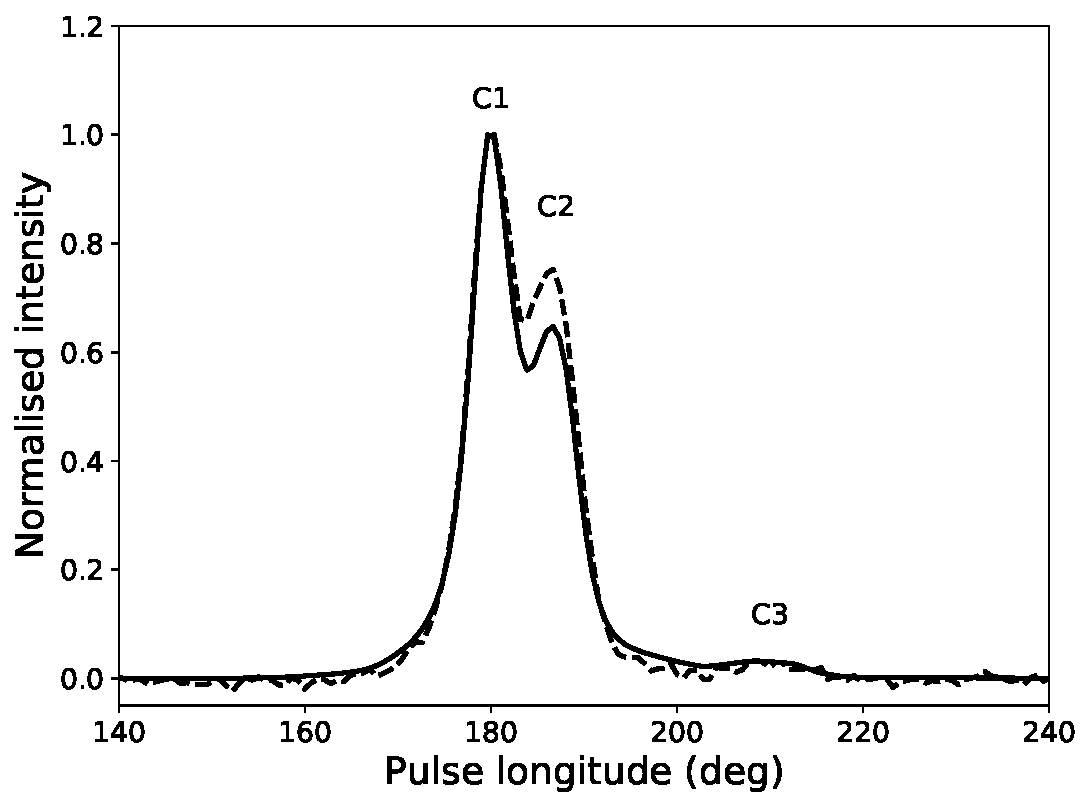
\includegraphics[width=0.6\textwidth]{Figures/J1518/profile_comparison}
        \caption[Profile comparison]{A comparison of the profile of PSR~J1518+4904 at 1250~MHz (solid line) with an archival profile at 1410~MHz \citep[dashed line,][]{KXL+1998}. Three main profile components are visible, labelled C1, C2, and C3 respectively. The small differences between the FAST data and the archival data are likely mostly spectral evolution (see the middle panel of Fig.~\ref{fig: J1518 - profile frequency evolution}).}
        \label{fig: J1518 - profile comparison}
    \end{center}
\end{figure}
The FAST profile is shown by the solid line while the archival observation is shown by the dashed line. Both profiles are normalised to their peak intensities, and are aligned by performing a cross-correlation using the \texttt{pmod} tool in \textsc{psrsalsa}. The pulse longitude range is cropped to show the detail of the main profile and its three components, C1, C2, and C3, which are labelled accordingly. There is little difference in the shape of the profiles, which indicates that we are safe to treat the FAST observation as though it is Stokes $I$. The slight difference in the relative intensity of component C2 could be entirely because of the difference in frequency of the two observations, as the profile does evolve with frequency as shown later in this section (the middle panel of Fig.~\ref{fig: J1518 - profile frequency evolution}).

\subsection{The pulse profile}
\label{sec: J1518 - analysis - new profile component}

The full-width integrated pulse profile of PSR~J1518+4904 is shown in the left-hand panel of Fig.~\ref{fig: J1518 - integrated profile}. The three observations which are unaffected by RFI are plotted together, with 2018-07-22 represented by the black line, 2018-08-04 the blue line, and 2018-11-04 the red line. The 2018-11-04 profile was aligned such that its peak lies at a longitude of $180\degr$. As it has the highest S/N, this profile was then used as a template to align the other two profiles by cross-correlation. All three profiles were normalised to a peak intensity of unity to aid visual comparison. No absolute flux calibration was possible for these commissioning data.
\begin{figure}
    \begin{center}
        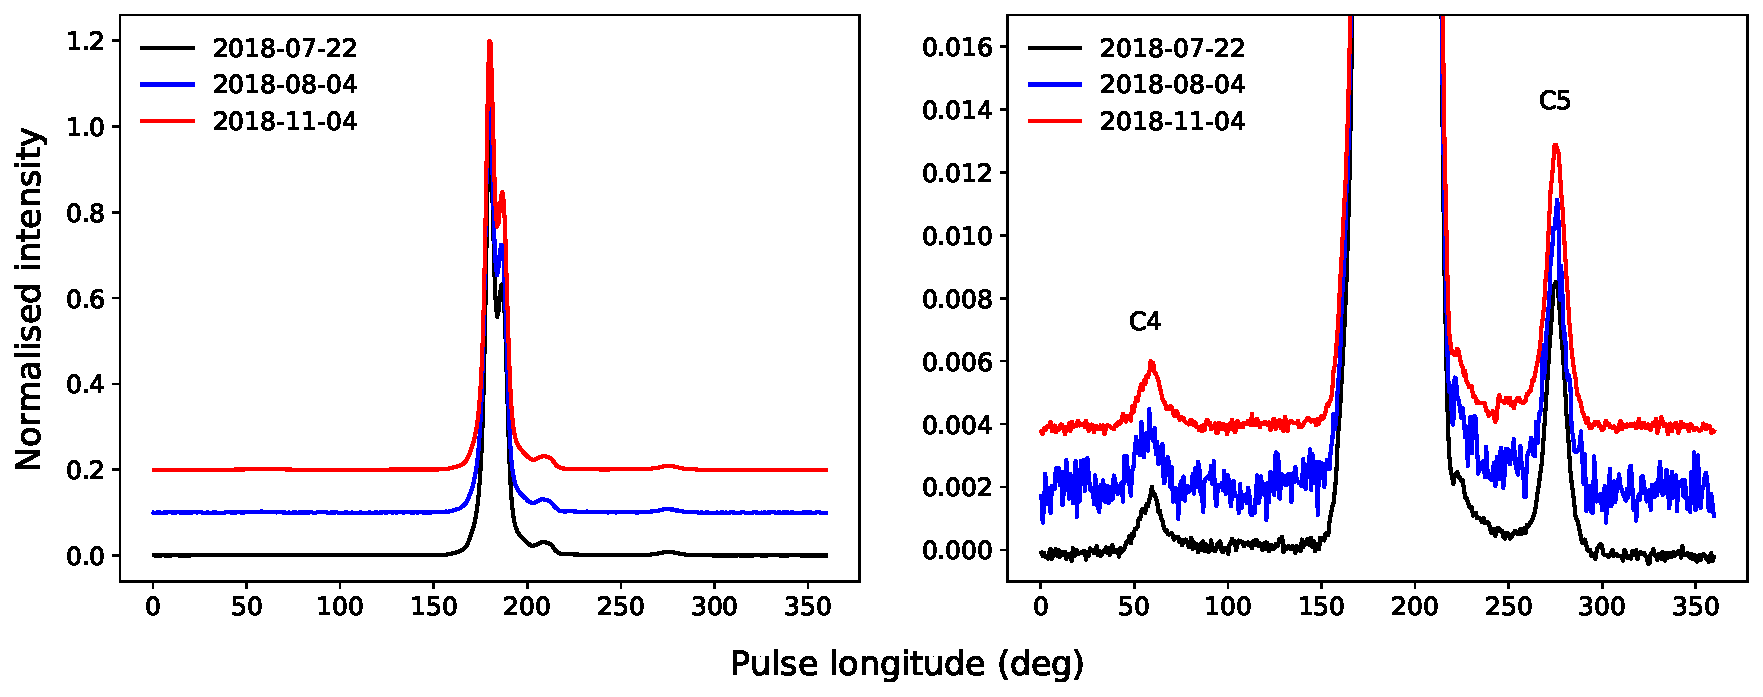
\includegraphics[width=1.0\textwidth]{Figures/J1518/profile_components}
        \caption[New profile components in PSR~J1518+4904]{(LEFT) The normalised profile of PSR~J1518+4904 (integrated over time and frequency) as observed at three different epochs, as indicated by the line colour. (RIGHT) The same profiles, but cropped to low intensities in order to highlight the weak profile components around $55\degr$ and $275\degr$ in pulse longitude, labelled C4 and C5 respectively. To aid comparison the different observations have been plotted with small vertical offsets.}
        \label{fig: J1518 - integrated profile}
    \end{center}
\end{figure}

The excellent sensitivity of FAST means that two new profile components could be identified. They are significantly weaker than the main component, around 0.9 and 0.2~per~cent respectively of the peak amplitude. The right-hand panel of Fig.~\ref{fig: J1518 - integrated profile} shows the same set of profiles as the left-hand panel, but cropped to one~per~cent of the peak intensity to highlight the newly identified components. The weaker of the new components is centred on $\sim$59$\degr$ pulse longitude, whilst the stronger lies at $275\degr$. This second new component is clearly connected to the main profile via a weak bridge of emission, while this is less clear for the weakest component. Both new components appear in all three observations with the same relative amplitude to the main peak, so they are confirmed to be stable profile features across a period of at least four months. The new leading component is too weak for it to be identified in the single-pulse data, but the new trailing component is faintly detectable.

\begin{figure}
    \begin{center}
        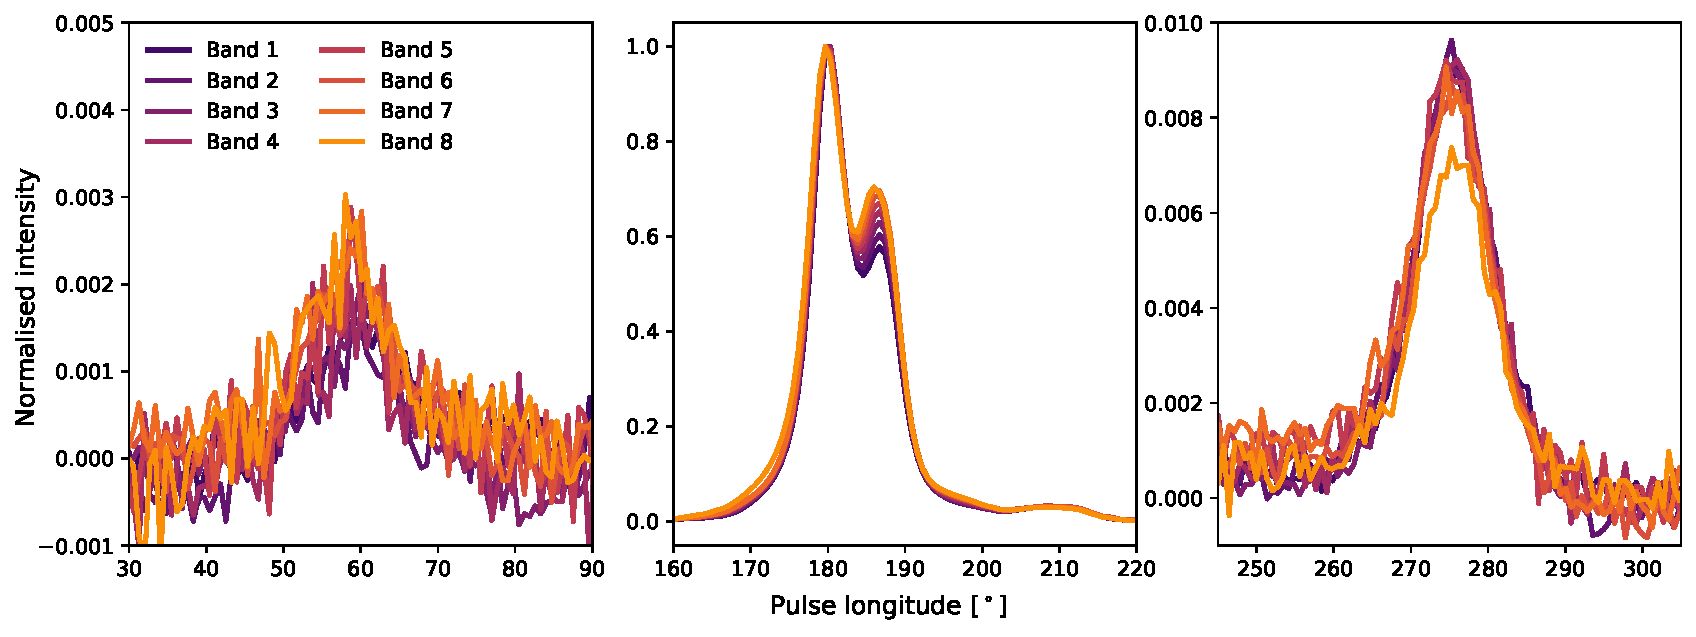
\includegraphics[width=1.0\textwidth]{Figures/J1518/profile_freq_evolution}
        \caption[Frequency evolution of profile components]{The frequency evolution of the three profile components across the eight sub-bands of the 2018-11-04 observation, shown here because it has the highest S/N profile due to its increased length -- the 2018-07-22 and 2018-08-04 observations are consistent. The weaker new component is shown in the left-hand panel (cropped to 0.5~per~cent of the main peak intensity to show the component more clearly). The main profile components are shown in the middle panel -- all eight sub-bands were normalised with respect to the amplitude of the main peak. The stronger new component at later pulse longitudes is shown in the right-hand panel. Neither of the new components appear to significantly change with frequency, but the intensity of the secondary peak of the main component gradually increases with frequency compared to the main peak.}
        \label{fig: J1518 - profile frequency evolution}
    \end{center}
\end{figure}

As illustrated by Fig.~\ref{fig: J1518 - profile frequency evolution}, the shape and relative amplitude of the new components are also stable across the 500~MHz frequency range covered by these observations. This figure shows a close-up view of the weak new component (left-hand panel), the main profile (centre panel), and the stronger new component (right-hand panel) across all eight frequency sub-bands in the 2018-11-04 observation. These are plotted in order of increasing frequency, in the colour gradient from deep purple to light orange. The weak new component appears relatively stable, and shows a possible slight increase in intensity with increasing frequency, but this is not significant. Similarly, the stronger new component (right-hand panel) appears unchanged across the frequency range, with the exception of band 8 (lightest orange) which appears attenuated. This suggests a rapid profile evolution starting to take place at the top end of the frequency range covered.

In the main profile (middle panel of Fig.~\ref{fig: J1518 - profile frequency evolution}), at least three distinct components are visible. The profiles are normalised to the leading, brightest, component ($180\degr$) so its frequency evolution is by definition removed. The weakest, trailing, component ($\sim$210$\degr$) does not appear to evolve with frequency. However, the middle component ($\sim$187$\degr$) appears to increase in intensity with increasing frequency relative to the main peak by a factor of approximately 1.3. The wings of the main peak (around $170\degr$ and $195\degr$) also show a slight trend of broadening with frequency. In all three panels, there is no indication that the peaks shift relative to one another in longitude with frequency, so the overall width and structure of the profile remains constant across the bandwidth. 

It should be stressed that because the profiles are normalised to the peak of the profile, only \textit{relative} changes can be detected. Also, because the data is not polarisation-calibrated, the shape of the profile could be somewhat distorted. It can not be ruled out that some of the frequency dependence in the profile shape is related to Faraday rotation. The linear and circular polarisation fractions are approximately 20~per~cent at 1410~MHz \citep{XKJ+1998}, with the (left-handed) circularly polarised emission associated with profile component C1, and the linearly polarised emission with profile component C2. The rotation measure of PSR~J1518+4904 is RM $= -15.6 \pm 3.7$~rad~m$^{-2}$ \citep{NPN+2020}, which means that the expected change in position angle $\Delta\psi \approx 45\degr$ across the observed bandwidth (see Sec.~\ref{sec: intro - observation processing - ISM effects - faraday rotation}), so Faraday rotation will be important to correct when studying the polarisation properties of this pulsar with FAST.

However, given the consistency of the different observations, in combination with the fact that this source is known to have only a modest degree of polarisation, this suggests that the main effect is profile evolution in Stokes $I$. The stronger new profile component extends the main profile width of PSR~J1518+4904 by a factor of $\sim$4, whilst the weaker one is sufficiently separated to be consistent with an interpulse. This new profile structure and its implications are discussed in Sec.~\ref{sec: J1518 - discussion}.








\subsection{Longitude-resolved fluctuation spectrum, LRFS}
\label{sec: J1518 - analysis - LRFS}

% \begin{wrapfigure}[20]{o}{0.4\textwidth}
\begin{figure}
    \begin{center}
        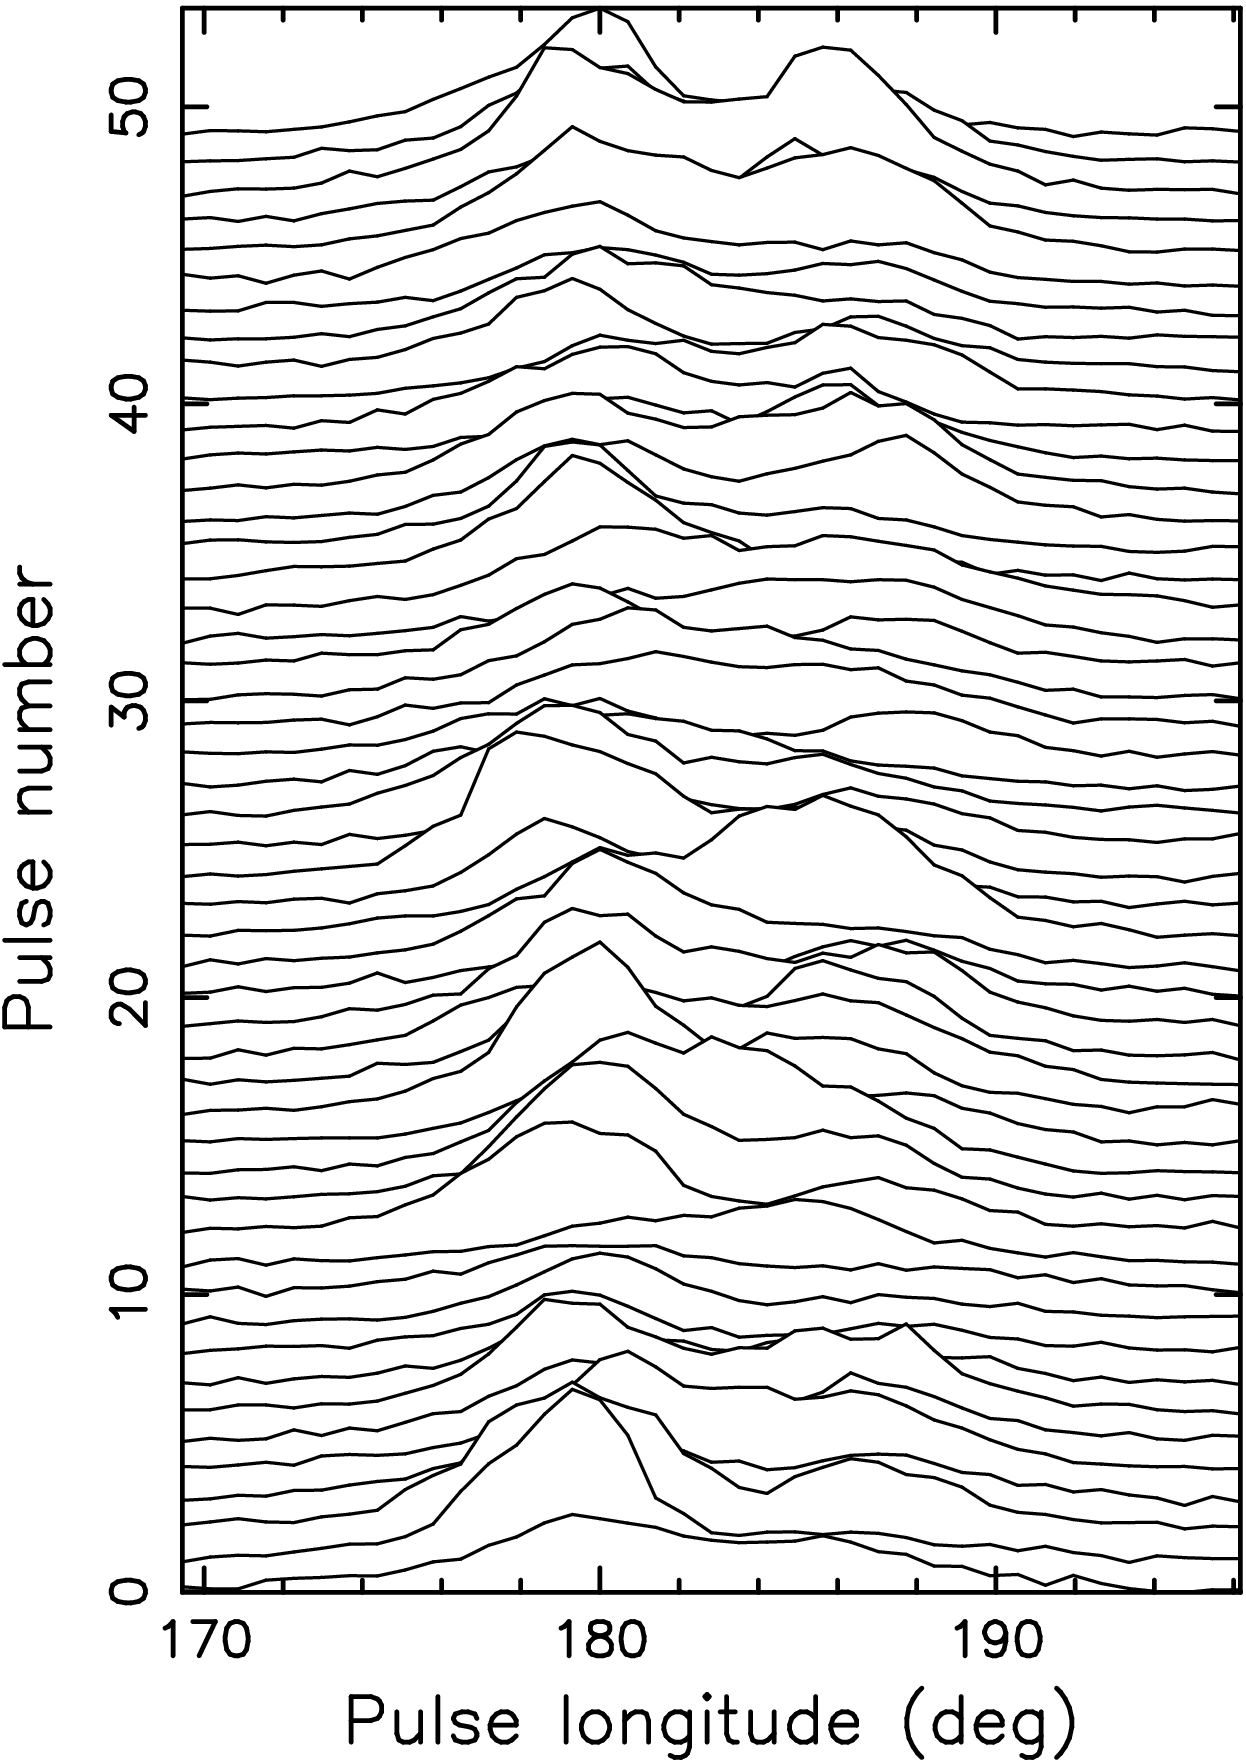
\includegraphics[width=0.4\textwidth]{Figures/J1518/stack_joy.png}
        \caption[Single pulses of PSR~J1518+4904]{A short stack of 50 pulses of PSR~J1518+4904 as observed with FAST on 2018-11-04 to illustrate how well the single pulses can be seen. Subpulse drift is occurring, but too rapidly for distinct driftbands to be resolved.}
        \label{fig: J1518 - short stack}
    \end{center}
\end{figure}
% \end{wrapfigure}
In contrast to previous studies of PSR~J1518+4904, our observations with FAST with its exceptional gain are sensitive enough to clearly detect single pulses, which means that fluctuation analysis of this MSP is possible in unprecedented detail. The quality of our data is illustrated in Fig.~\ref{fig: J1518 - short stack} which shows a short sequence of individual pulses cropped to focus on the main peak.

A longitude-resolved fluctuation spectrum (LRFS) was produced for each of the three analysed observations according to the method detailed in Sec.~\ref{sec: J1926 - analysis - single pulse variability}. The length of the Fourier transform used to calculate the LRFS was 1024 pulses, and all pulses were used for each epoch. Figure~\ref{fig: J1518 - lrfs time evolution} shows a magnified view of two pulse longitude regions of the LRFS for each observation.
The left-hand panels show the LRFS between longitudes $176\degr$ and $190\degr$ (covering profile components C1 and C2) whilst the right-hand panels show the region between $192\degr$ and $212\degr$ (between profile components C2 and C3). No significant periodic modulation was detected in the regions occupied by the new profile components. Although the two columns in the figure form a continuous longitude range, they are separated to allow the weaker spectral features at later longitudes to stand out better by having different dynamic ranges in the two sets of plots. The 2018-07-22 observation is shown in the top two panels, 2018-08-04 in the middle row, and 2018-11-04 in the bottom row. Each of the six plots is accompanied by a side panel (line plot) which shows the integrated power spectrum over the displayed longitude range.

\begin{figure}
    \begin{center}
        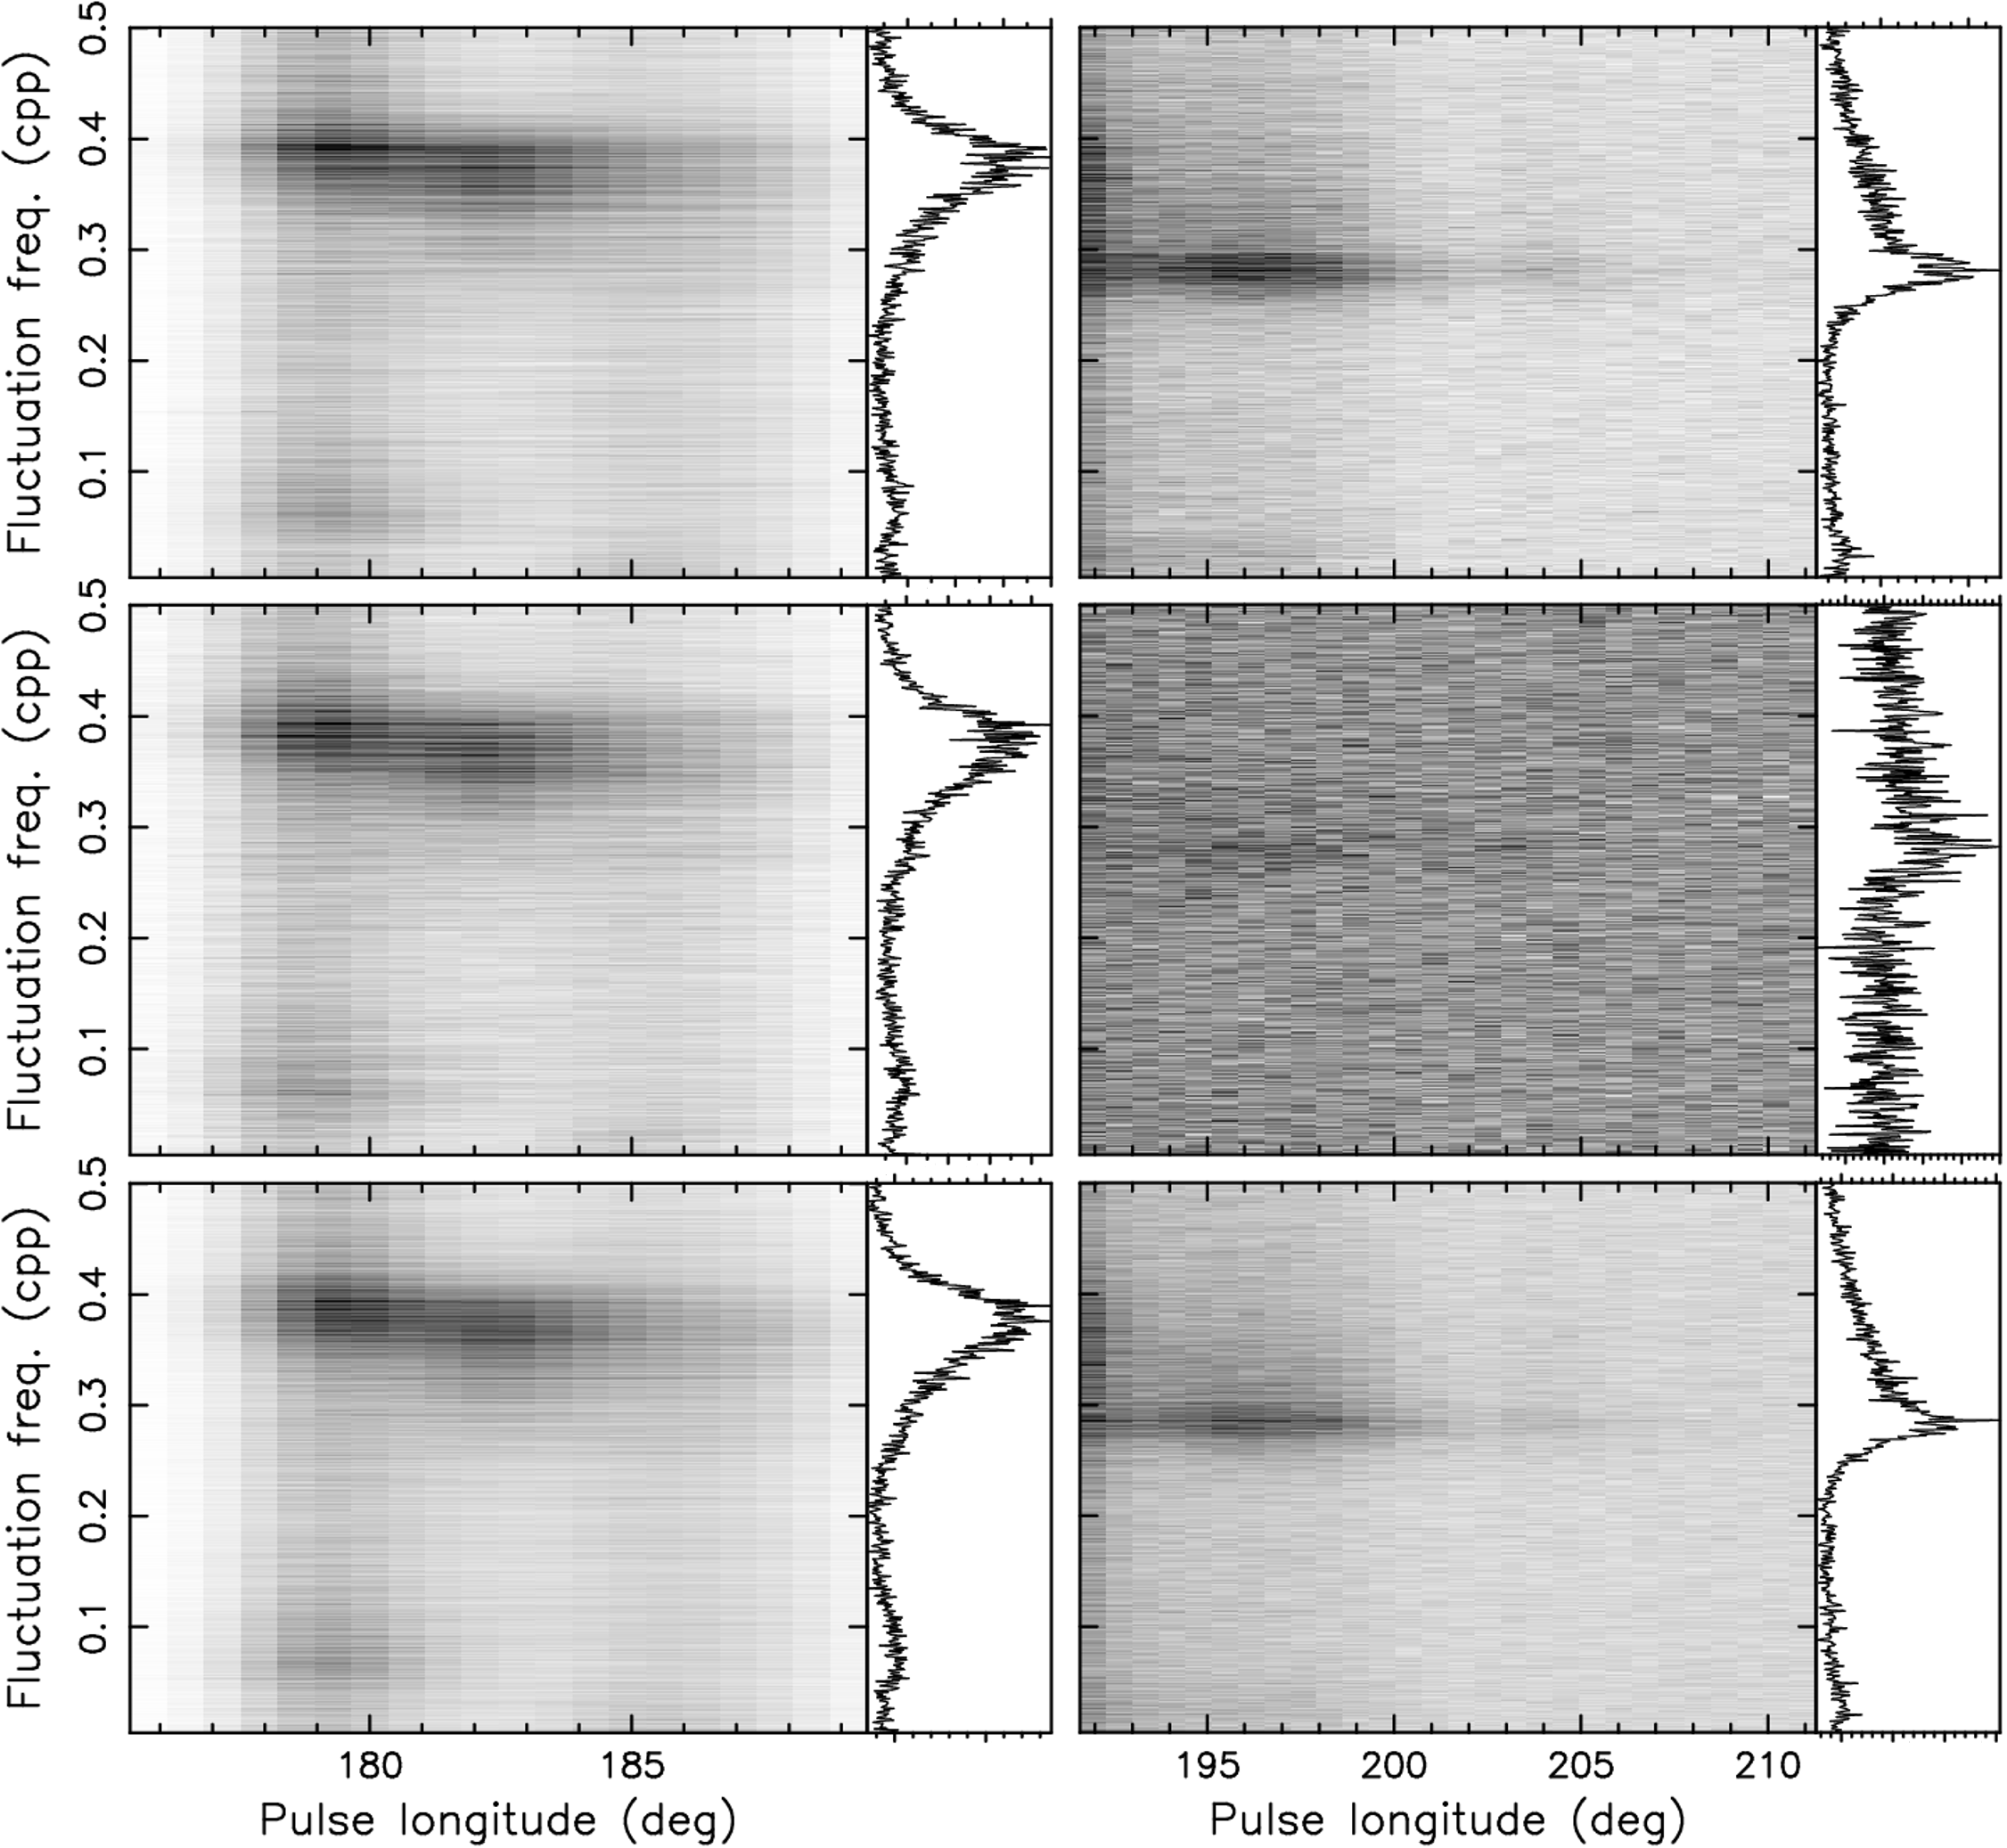
\includegraphics[width=1.0\textwidth]{Figures/J1518/lrfs_time_evolution_2}
        \caption[Longitude-resolved fluctuation spectra of PSR~J1518+4904]{The LRFS of PSR~J1518+4904 at three different epochs: 2018-07-22 (top row), 2018-08-04 (middle row), and 2018-11-04 (bottom row). The left-hand panels show the power spectrum between pulse longitudes $176\degr$ and $190\degr$, whilst the right-hand panels show the spectrum between longitudes $192\degr$ and $212\degr$. The fluctuation power in the earlier pulse longitudes strongly dominates that of the later longitudes, so they are shown separately. Two $P_3$ features are seen in the left-hand panels, the strongest peaking around 0.38~cpp and a fainter peak at around 0.07~cpp which is constrained to profile component C1. The spectrum of the later longitudes exhibits a single distinct $P_3$ peak at $\sim$0.29~cpp which appears in all three epochs (albeit only faintly in 2018-08-04).}
        \label{fig: J1518 - lrfs time evolution}
    \end{center}
\end{figure}

The left-hand panels show a very strong, broad spectral feature peaking at around 0.38 cycles per period (cpp) which extends across the displayed pulse longitude range. It covers the two brightest profile components, seen most clearly in the central panel of Fig.~\ref{fig: J1518 - profile frequency evolution}. There is a second, fainter spectral feature which is strongest between $178\degr$ and $180\degr$ pulse longitude and peaks at approximately $0.07$~cpp. This longer-period modulation appears to be localised within the brightest component C1 of the main peak of the profile. The features in the left-hand panels of Fig.~\ref{fig: J1518 - lrfs time evolution} are both quite broad in $P_3$, which indicates that although the pulse-to-pulse variability is periodic, the periodicity is somewhat irregular.

The right-hand panels of Fig.~\ref{fig: J1518 - lrfs time evolution} show the section of the LRFS that covers the longitude range occupied by the trailing shoulder of the main profile. The 2018-07-22 and 2018-11-04 observations (top and bottom panels) both show a somewhat more well-defined peak at around 0.28~cpp. The peak is quite asymmetric, with a long tail towards 0.5~cpp. This is best seen at the early side of the longitude range. The peak is also faintly visible in the 2018-08-04 observation (middle panel). This observation has a significantly lower signal-to-noise ratio than the other two (see the right hand panel of Fig.~\ref{fig: J1518 - lrfs time evolution}). Nevertheless, compared to the periodic modulation at earlier longitudes (left-hand panel), it seems that the 0.28~cpp modulation is significantly weaker during this epoch without the overall relative intensity of the profile at this pulse longitude range being affected (see Fig.~\ref{fig: J1518 - integrated profile}).

Although they are connected in pulse longitude, the periodicities in the pulse-to-pulse modulation are distinctly different in the two regions. In addition, the periodicity seems to shift with pulse longitude in the left-hand panels as well. This will be described and discussed further in Sec.~\ref{sec: J1518 - discussion - funky P3}.
Figure~\ref{fig: J1518 - lrfs time evolution} shows that the main features in the LRFS of PSR~J1518+4904 are stable over the period over which the different observations took place. In order to investigate the stability of the features as a function of frequency, the LRFS was explored for the eight sub-bands of the 2018-11-04 observation. These results are shown in Fig.~\ref{fig: J1518 - lrfs freq evolution}, which are similar to Fig.~\ref{fig: J1518 - lrfs time evolution}, except that two panels are shown per frequency sub-band (the sub-band label is shown in the top-left of each panel in the first and third columns). It is evident that the main features of the LRFS are independent of frequency. This is a general property of drifting subpulses, where the periodicity $P_3$ is observed to be independent of frequency \citep{WSEx2007}. It also rules out that these spectral features are because of incidental narrowband RFI (although the fact that the features are not found in the off-pulse region also rules that out).




\begin{landscape}
    \begin{figure}
        \begin{center}
            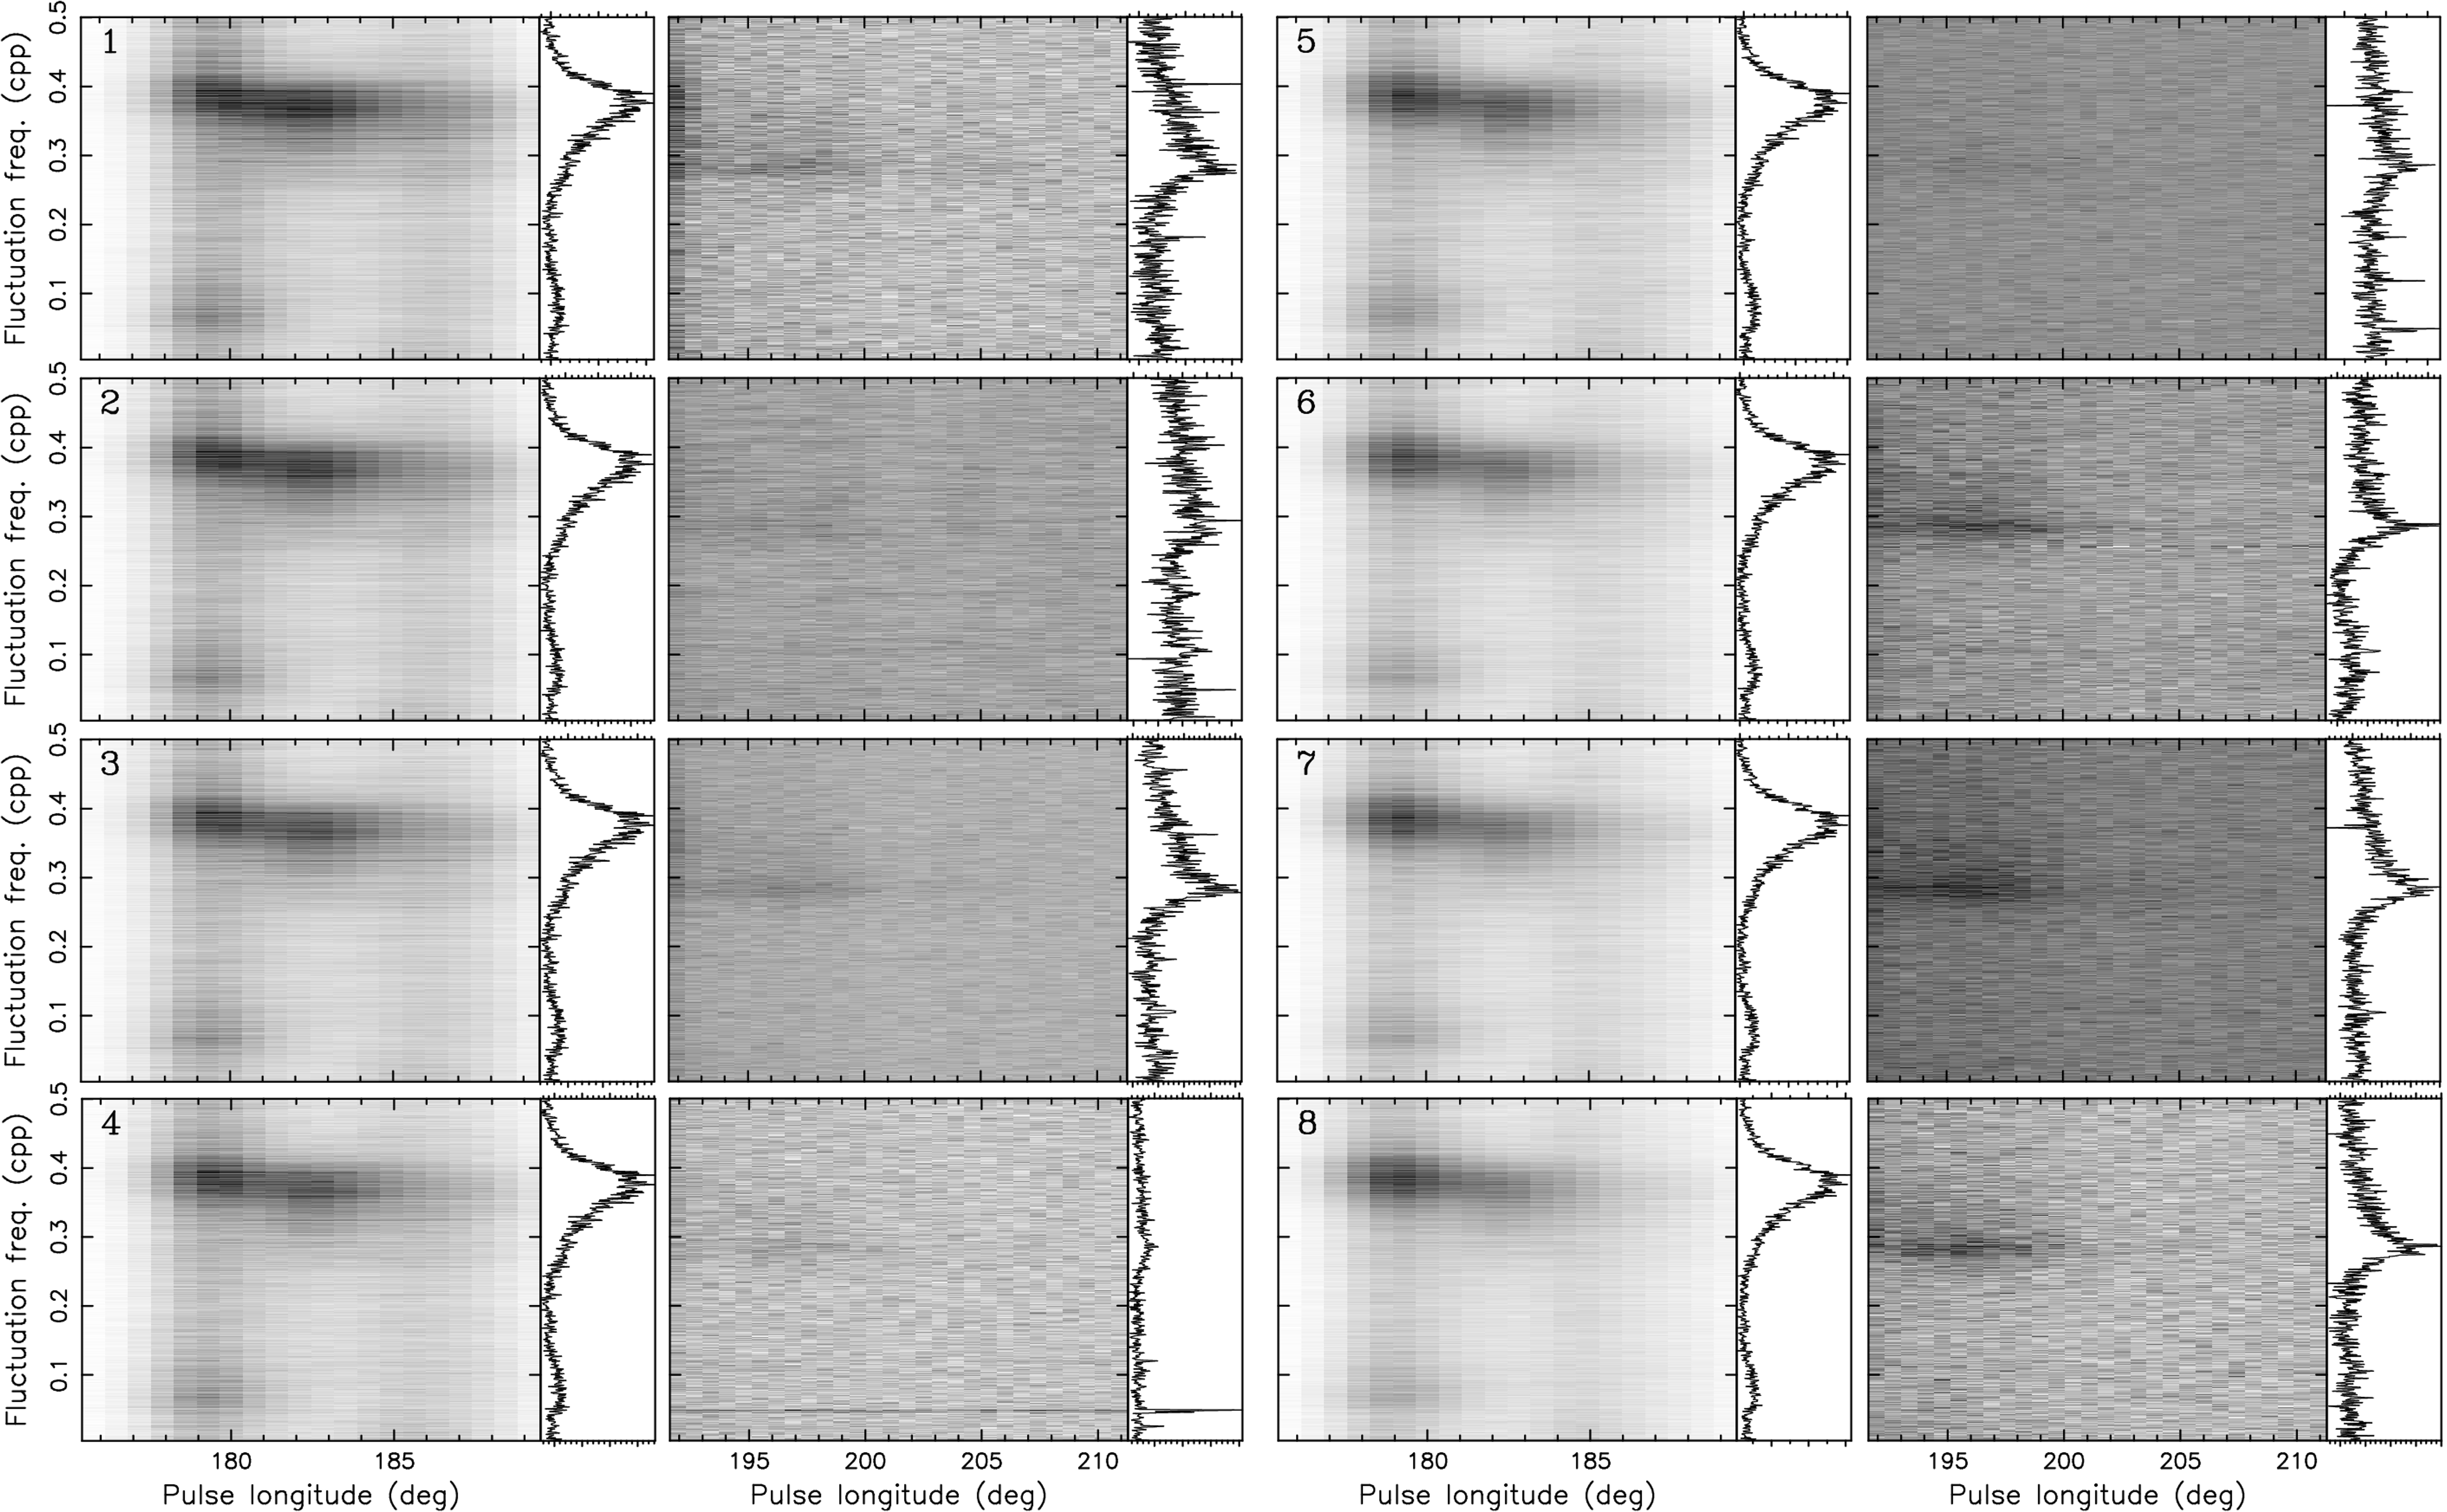
\includegraphics[width=0.82\textheight]{Figures/J1518/lrfs_freq_evolution_2}
            \caption[Frequency evolution of the LRFS]{The frequency evolution of the two components of the LRFS across the 2018-11-04 observation, where the two panels per frequency band are as described in Fig.~\ref{fig: J1518 - lrfs time evolution}. The frequency band number is shown in the top-left corner of panels corresponding to the spectrum of the main component. The frequencies covered by the sub-bands are defined in Table~\ref{tab: J1518 - frequency sub-bands}. Frequency increases with sub-band number. The main features of the LRFS are visible across the full frequency range.}
            \label{fig: J1518 - lrfs freq evolution}
        \end{center}
    \end{figure}
\end{landscape}




\subsection{Two-dimensional fluctuation spectrum, 2DFS}
\label{sec: J1518 - analysis - 2DFS}
\begin{figure}
    \begin{center}
        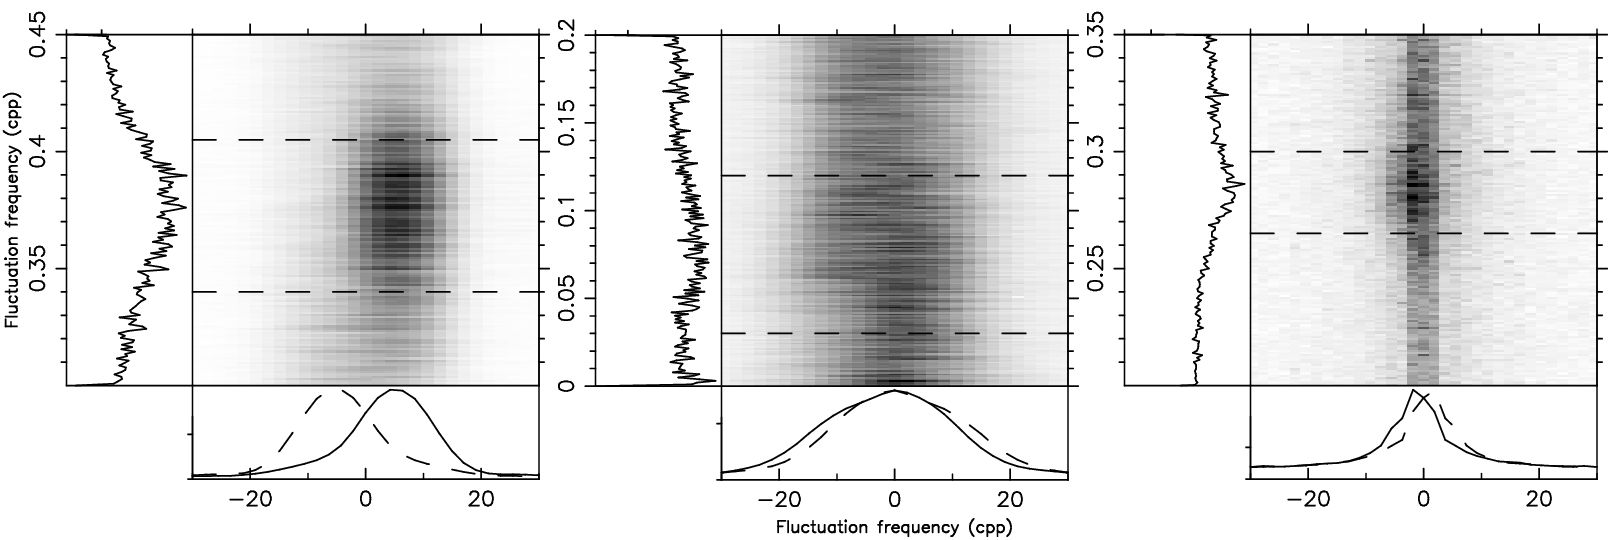
\includegraphics[width=\textwidth]{Figures/J1518/2DFS_all}
        \caption[2DFS of PSR~J1518+4904]{The 2DFS of PSR~J1518+4904, calculated from the 2018-11-04 observation. The left-hand and middle panels were calculated using a pulse longitude range of $102\degr$ to $191\degr$ (enclosing profile components C1 and C2), and the right-hand panel used longitudes from $194\degr$ to $1283\degr$ (C3). The shading shows the power at a given $P_1/P_2$ ($x$-axis) and $P_1/P_3$ ($y$-axis) fluctuation frequency, with more power shown as darker grey. The line plot to the side of each panel shows the $P_1/P_3$ distribution integrated horizontally across the window, and the solid lines in the line plots below show the $P_1/P_2$ distribution integrated vertically between the horizontal dashed lines. The dashed line in the lower line plots shows the $P_1/P_2$ distribution reflected about $P_1/P_2 = 0$ to highlight any asymmetry.}
        \label{fig: J1518 - 2DFS}
    \end{center}
\end{figure}

A 2DFS as described in Sec.~\ref{sec: J1926 - analysis - single pulse variability} was created for PSR~J1518+4904, using the 2018-11-04 observation. Unlike the LRFS, which is only sensitive to fluctuation periodicities from pulse to pulse ($P_3$), the 2DFS is also sensitive to longitudinal drift associated with these periodicities ($P_2$). Figure~\ref{fig: J1518 - 2DFS} shows the 2DFS calculated for the three features seen in the LRFS, at 0.38~cpp (left panel), 0.07~cpp (centre panel) and 0.28~cpp (right panel) respectively. The three panels have been cropped to show the $P_3$ range of interest for each feature: the line plots in the panels to the left of each plot show the integrated $P_3$ power spectrum, and the solid line plots beneath each plot show the $P_2$ power spectrum integrated between the horizontal dashed lines which delimit the location of the features in $P_3$. The dashed lines in the same panels show the integrated $P_2$ peak reflected about $P_1/P_2 = 0$~cpp in order to highlight any asymmetry.

Using the \texttt{pspecDetect} tool in \textsc{psrsalsa}, the position of the features in the 2DFS were quantified. For the 0.38~cpp feature, the centroid is located at $P_2 = 69\degr \pm 1 \degr$, and $P_3 = 2.660 \pm 0.005\ P_1$. The centroid of the 0.28~cpp feature is at $P_2 = -250\degr \pm 40 \degr$, and $P_3 = 3.51 \pm0.02\ P_1$. The 0.07~cpp feature in the middle panel is weak, without it standing out from the non-periodic modulation power in the 2DFS, but the asymmetry of its $P_2$ spectrum implies a slightly negative $P_2$, indicating drifting. The sign of $P_2$ indicates the direction of drift: a positive $P_2$ shows that subpulses are moving towards later longitudes, or from left to right across the profile. The drift rate is given by $D=P_2 / P_3$, so for the 0.38~cpp component $D=+25.9\pm0.4$~$\degr/P_1$, and for the 0.28~cpp component $D = -70 \pm 10$~$\degr/P_1$. Both of these are exceptionally rapid drift rates, implying the modulation is almost `longitude stationary', i.e. modulation where the driftbands are practically horizontal. The values of $P_1/P_2 = 10$~cpp and $P_1/P_3 = 0.38$~cpp were previously determined by \citet{ESxx2003} (see Sec.~\ref{sec: J1518 - intro}) -- their value of $P_2$ differs from our own, possibly because they use the full pulse profile in their calculation (whereas we separate the components with different periodicities) which could effectively average $P_2$ of the different components and reduce the apparent drift rate. 

The periodic modulation is relatively imprecise, and because of the additional non-periodic modulation, the drifting subpulses are difficult to recognise in a pulse stack (see Fig.~\ref{fig: J1518 - short stack}). However, they are clearly detected in the statistical analysis such as with the 2DFS. It is exceptional that the  drift features are moving in opposite directions (they have different signs of $P_2$), especially in the same component. This will be further discussed in Sec.~\ref{sec: J1518 - discussion - funky P3}.















\subsection{Longitude-dependence of \texorpdfstring{$P_3$}{P3}}
\label{sec: J1518 - analysis - drifting P3}
\begin{figure}
    \begin{center}
        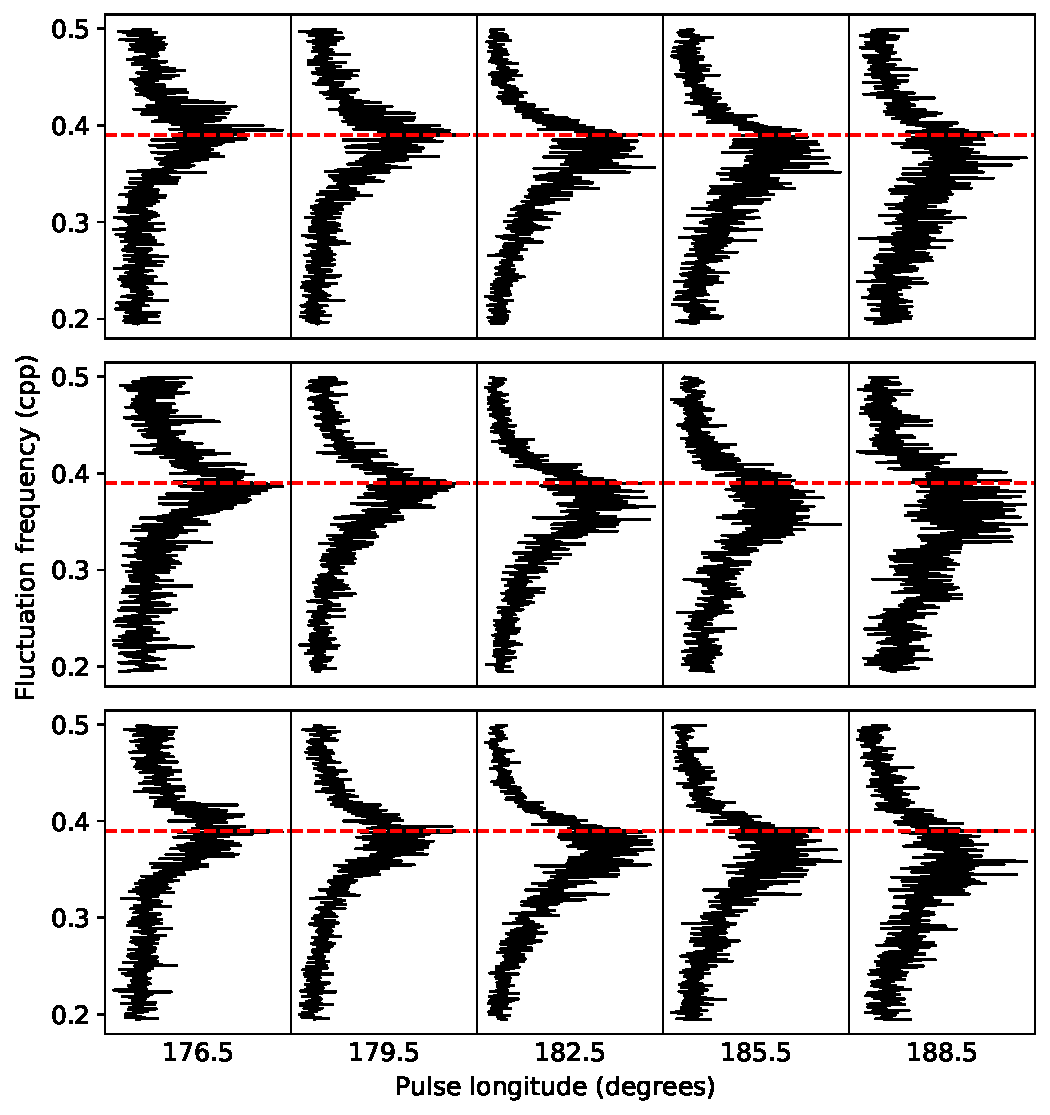
\includegraphics[width=0.55\textwidth]{Figures/J1518/drifting_P3}
        \caption[Drifting $P_3$ values in the main profile components]{The shift in the modulation frequency corresponding to $P_3$ across profile components C1 and C2, which is present in all epochs (top row -- 2018-07-22; middle row -- 2018-08-04; bottom row -- 2018-11-04). A range of pulse longitude of $15\degr$ between $175\degr$ and $190\degr$ was divided into $3\degr$ blocks, and the longitude-integrated LRFS (between 0.2 and 0.5~cpp) for each is shown from left to right (their central pulse longitude is shown on the $x$-axis). The red line indicates the peak of the earliest spectrum.}
        \label{fig: J1518 - drifting P3 components}
    \end{center}
\end{figure}

The dominant LRFS peak at $0.38$~cpp associated with profile components C1 and C2 appears to show a slight, but clear, evolution with pulse longitude, moving towards lower modulation frequencies as longitude increases while the spectral feature itself also becomes broader. This was investigated for all three epochs by dividing the LRFS into five blocks covering $3\degr$ in pulse longitude, between $175\degr$ and $190\degr$. These plots are shown in Fig.~\ref{fig: J1518 - drifting P3 components} -- as before, the top row shows the 2018-07-22 observation, the middle row is 2018-08-04, and the bottom row is 2018-11-04. All longitude bins across each $3\degr$-wide LRFS block were summed to produce the integrated spectra shown; their central pulse longitude is indicated on the $x$-axis. The displayed fluctuation frequencies have been limited to between 0.2 to 0.5~cpp in order to show the shift of the peak more clearly. This plot clearly demonstrates that the peak of the LRFS decreases in fluctuation frequency with increasing longitude by approximately $0.02$~cpp over the span, and this is the case for all three epochs. The red dashed line corresponds to a fluctuation frequency of 0.38~cpp, aligning with the peak of the spectrum at $176.5\degr$ (left-hand panels). The peak also becomes slightly broader with increasing longitude, and more noisy as a result of the decrease in spectral power with longitude. Overall, this seems to be part of a trend across the profile which ultimately leads to the modulation between profiles components C2 and C3 with a very different modulation period (0.28~cpp).  This is discussed further in Sec.~\ref{sec: J1518 - discussion - funky P3}.















\subsection{Evidence for disjoint drift modes}
\label{sec: J1518 - analysis - disjoint modes}

The existence of multiple discrete peaks in the LRFS as observed in other pulsars implies mode-switching, where the pulsar changes between different discrete drift states such that only one periodicity is visible at a given time in the pulse sequence. For example PSR~B0031$-$07 as described in Chapter~\ref{chapt: B0031} has three modes of drifting subpulses with modulation periods of $P_3 \approx 13P_1$, $P_3\approx 7P_1$ and $P_3 \approx 4P_1$ respectively. The pulsar abruptly switches between these modes. The modes have durations which have a characteristic timescale, but the distribution of durations is often broad. In addition, different profile components of pulsars are generally observed to share strictly identical periodicities. In PSR~J1518+4904 there are two discrete modulation periods in the leading component of the main peak (corresponding to 0.38 and 0.07~cpp). In addition, in the emission between components C2 and C3 a frequency corresponding to 0.28~cpp is present which is distinctly different from what is seen in the main pulse. Mode changes are known to occur with a wide range of timescales, typically on the order of minutes to hours, with the pulsar spending most of its time in the \textit{normal} mode and less frequently enters the \textit{abnormal} mode, with a distinctly different profile shape (e.g. \citealt{Sxxx2018} and references therein). Mode changing most commonly occurs in pulsars whose profiles comprise multiple components \citep{Rxxx1986}. The 2018-11-04 observation contains 88,400 single pulses, so there is certainly scope for two different drift modes occurring at different times to be present. The overarching question is if the different modulation periodicities occur simultaneously or if they are the result of mode changes. Since the LRFS is the average spectrum of the full observation, it cannot be used to distinguish between these two scenarios. 

Introduced by \citet{SSW+2009}, the sliding two-dimensional fluctuation spectrum (S2DFS) provides a way to study the time dependence of the fluctuation spectrum across the span of an observation. In this method fluctuation spectra are calculated as before, but with a slight difference. Instead of dividing the pulse stack up into equal-length blocks for which the power spectra are summed, the 2DFS is instead applied to a single window of $n$ pulses. The resulting spectrum is then collapsed in either the $P_2$ or $P_3$ direction, to create a one-dimensional spectrum for that block. The window of $n$ pulses is then shifted by one pulse and the process repeated. If the initial pulse stack consisted of $m$ pulses, then the result of the S2DFS is a `map' of $m-n+1$ collapsed spectra. This process allows any changes in the modulation to be resolved over timescales longer than $n$ pulses, the length of the discrete Fourier transform (DFT). A longer window can allow finer structures in the fluctuation spectra to be resolved, with the tradeoff of a reduced temporal resolution.

In this project, the individual fluctuation spectra were collapsed along the $P_2$ direction in order to attempt to resolve any evolution of $P_3$ during the observation. If PSR~J1518+4904 switches between drift modes with different periodicities on a timescale larger than the DFT size, then we can expect to observe spectral power alternating between distinct frequencies in the S2DFS. A DFT size of 256 pulses was chosen as a compromise between a sufficient spectral resolution without reducing the temporal resolution unnecessarily. Figure~\ref{fig: J1518 - S2DFS} shows a section of the S2DFS for the 2018-11-04 observation, over a span of 10,000 single pulses towards the end of the observation. This region was chosen because the pulsar was closer to the horizon at the start of the observation and its signal was weaker as a consequence, hence the modulation is less pronounced in earlier pulses. Nevertheless, this region is representative of what is observed over the full observation. The three panels show magnified regions of the S2DFS, which was computed for the three periodicities visible in the LRFS. The periodicity around 0.38~cpp is shown in the top panel, 0.28~cpp in the middle, and 0.07~cpp in the lower panel. The broadness (in frequency) of the spectral features in the in the LRFS can be understood as stochastic variability in the fluctuation frequency. The broad peaks in the right-hand side panels are the result of the addition of many narrow frequency features seen on short timescales. This variability seems erratic, with no resolved gradual systematic changes in the frequency as a function of time. Comparing the three panels, there is no evidence for switching such that only one of the main spectral features seen in the LRFS is visible at a given pulse-number interval. Therefore, the different modulation frequencies appear to be present at all times during the observation. The effect of the FFT length limiting the time resolution is evident -- one can see that the individual spectral features are smeared out slightly along the pulse number direction. If mode-switching happens on shorter timescales than the FFT length, it will not be resolved. So very rapid mode changes cannot be ruled out with this analysis.

\begin{figure}
    \begin{center}
        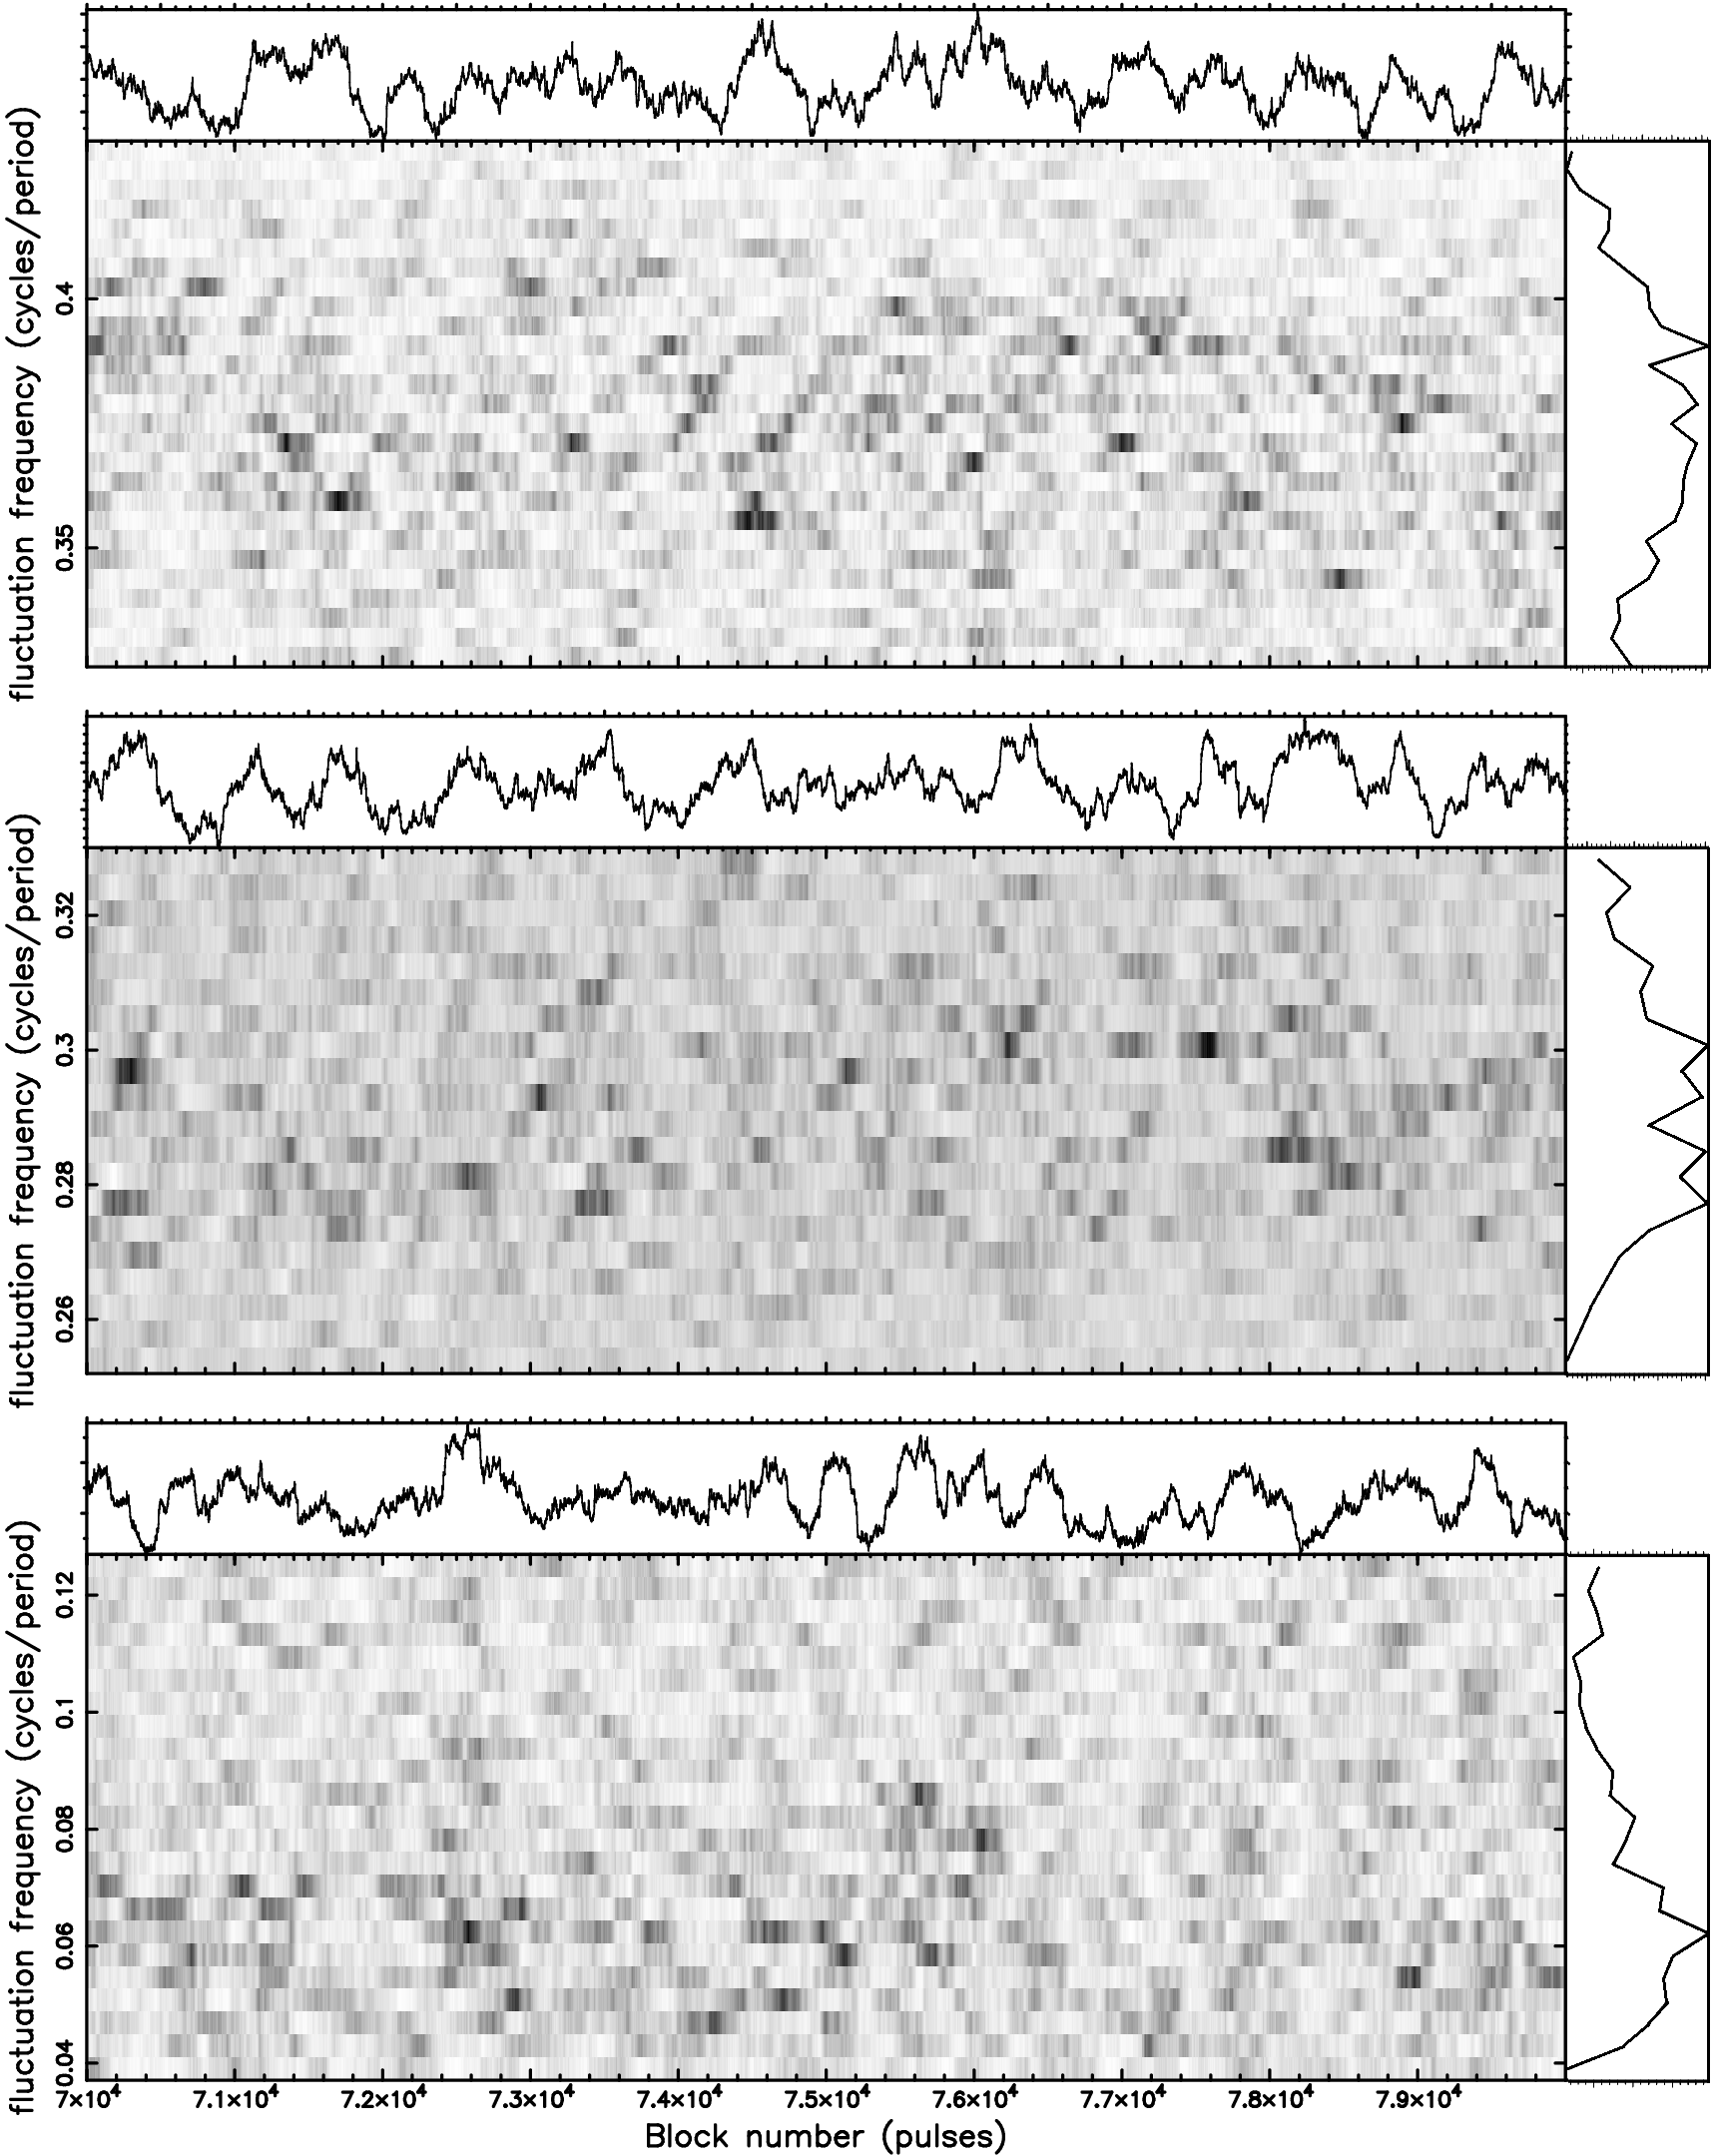
\includegraphics[width=1.0\textwidth]{Figures/J1518/S2DFS_256_2.png}
        \caption[The sliding 2DFS]{A section of the S2DFS for the 2018-11-04 observation, between pulse numbers 70,000 and 80,000. The three plots show different frequency ranges of the $P_3$ spectrum, cropped to show the feature at 0.38~cpp in the upper plot, 0.28~cpp in the middle, and 0.07~cpp in the lower panel. Alongside each greyscale plot, the top panel shows the total modulation power as a function of time, showing that $P_3$ varies stochastically within the envelope shown in the right-hand side panel. No mode switching is observed whereby only one of the three periodicities is seen at a given time.}
        \label{fig: J1518 - S2DFS}
    \end{center}
\end{figure}



As the S2DFS analysis proved inconclusive in showing the existence of distinct drift modes, an alternative method was explored. As shown by the LRFS (e.g. Fig.~\ref{fig: J1518 - lrfs time evolution}) the two $P_3$ features at 0.38~cpp and 0.28~cpp are associated with different pulse longitude ranges. In general drift mode changes are associated with changes in the shape of the average pulse profile. If this is the case in PSR~J1518+4904, then we might expect relative (correlated or anti-correlated) changes in intensity at the two distinct pulse longitude ranges. By calculating the flux density of the emission by integrating over the two ranges, we can look for a bimodality in a scatter plot of these two quantities.

\begin{figure}
    \begin{center}
        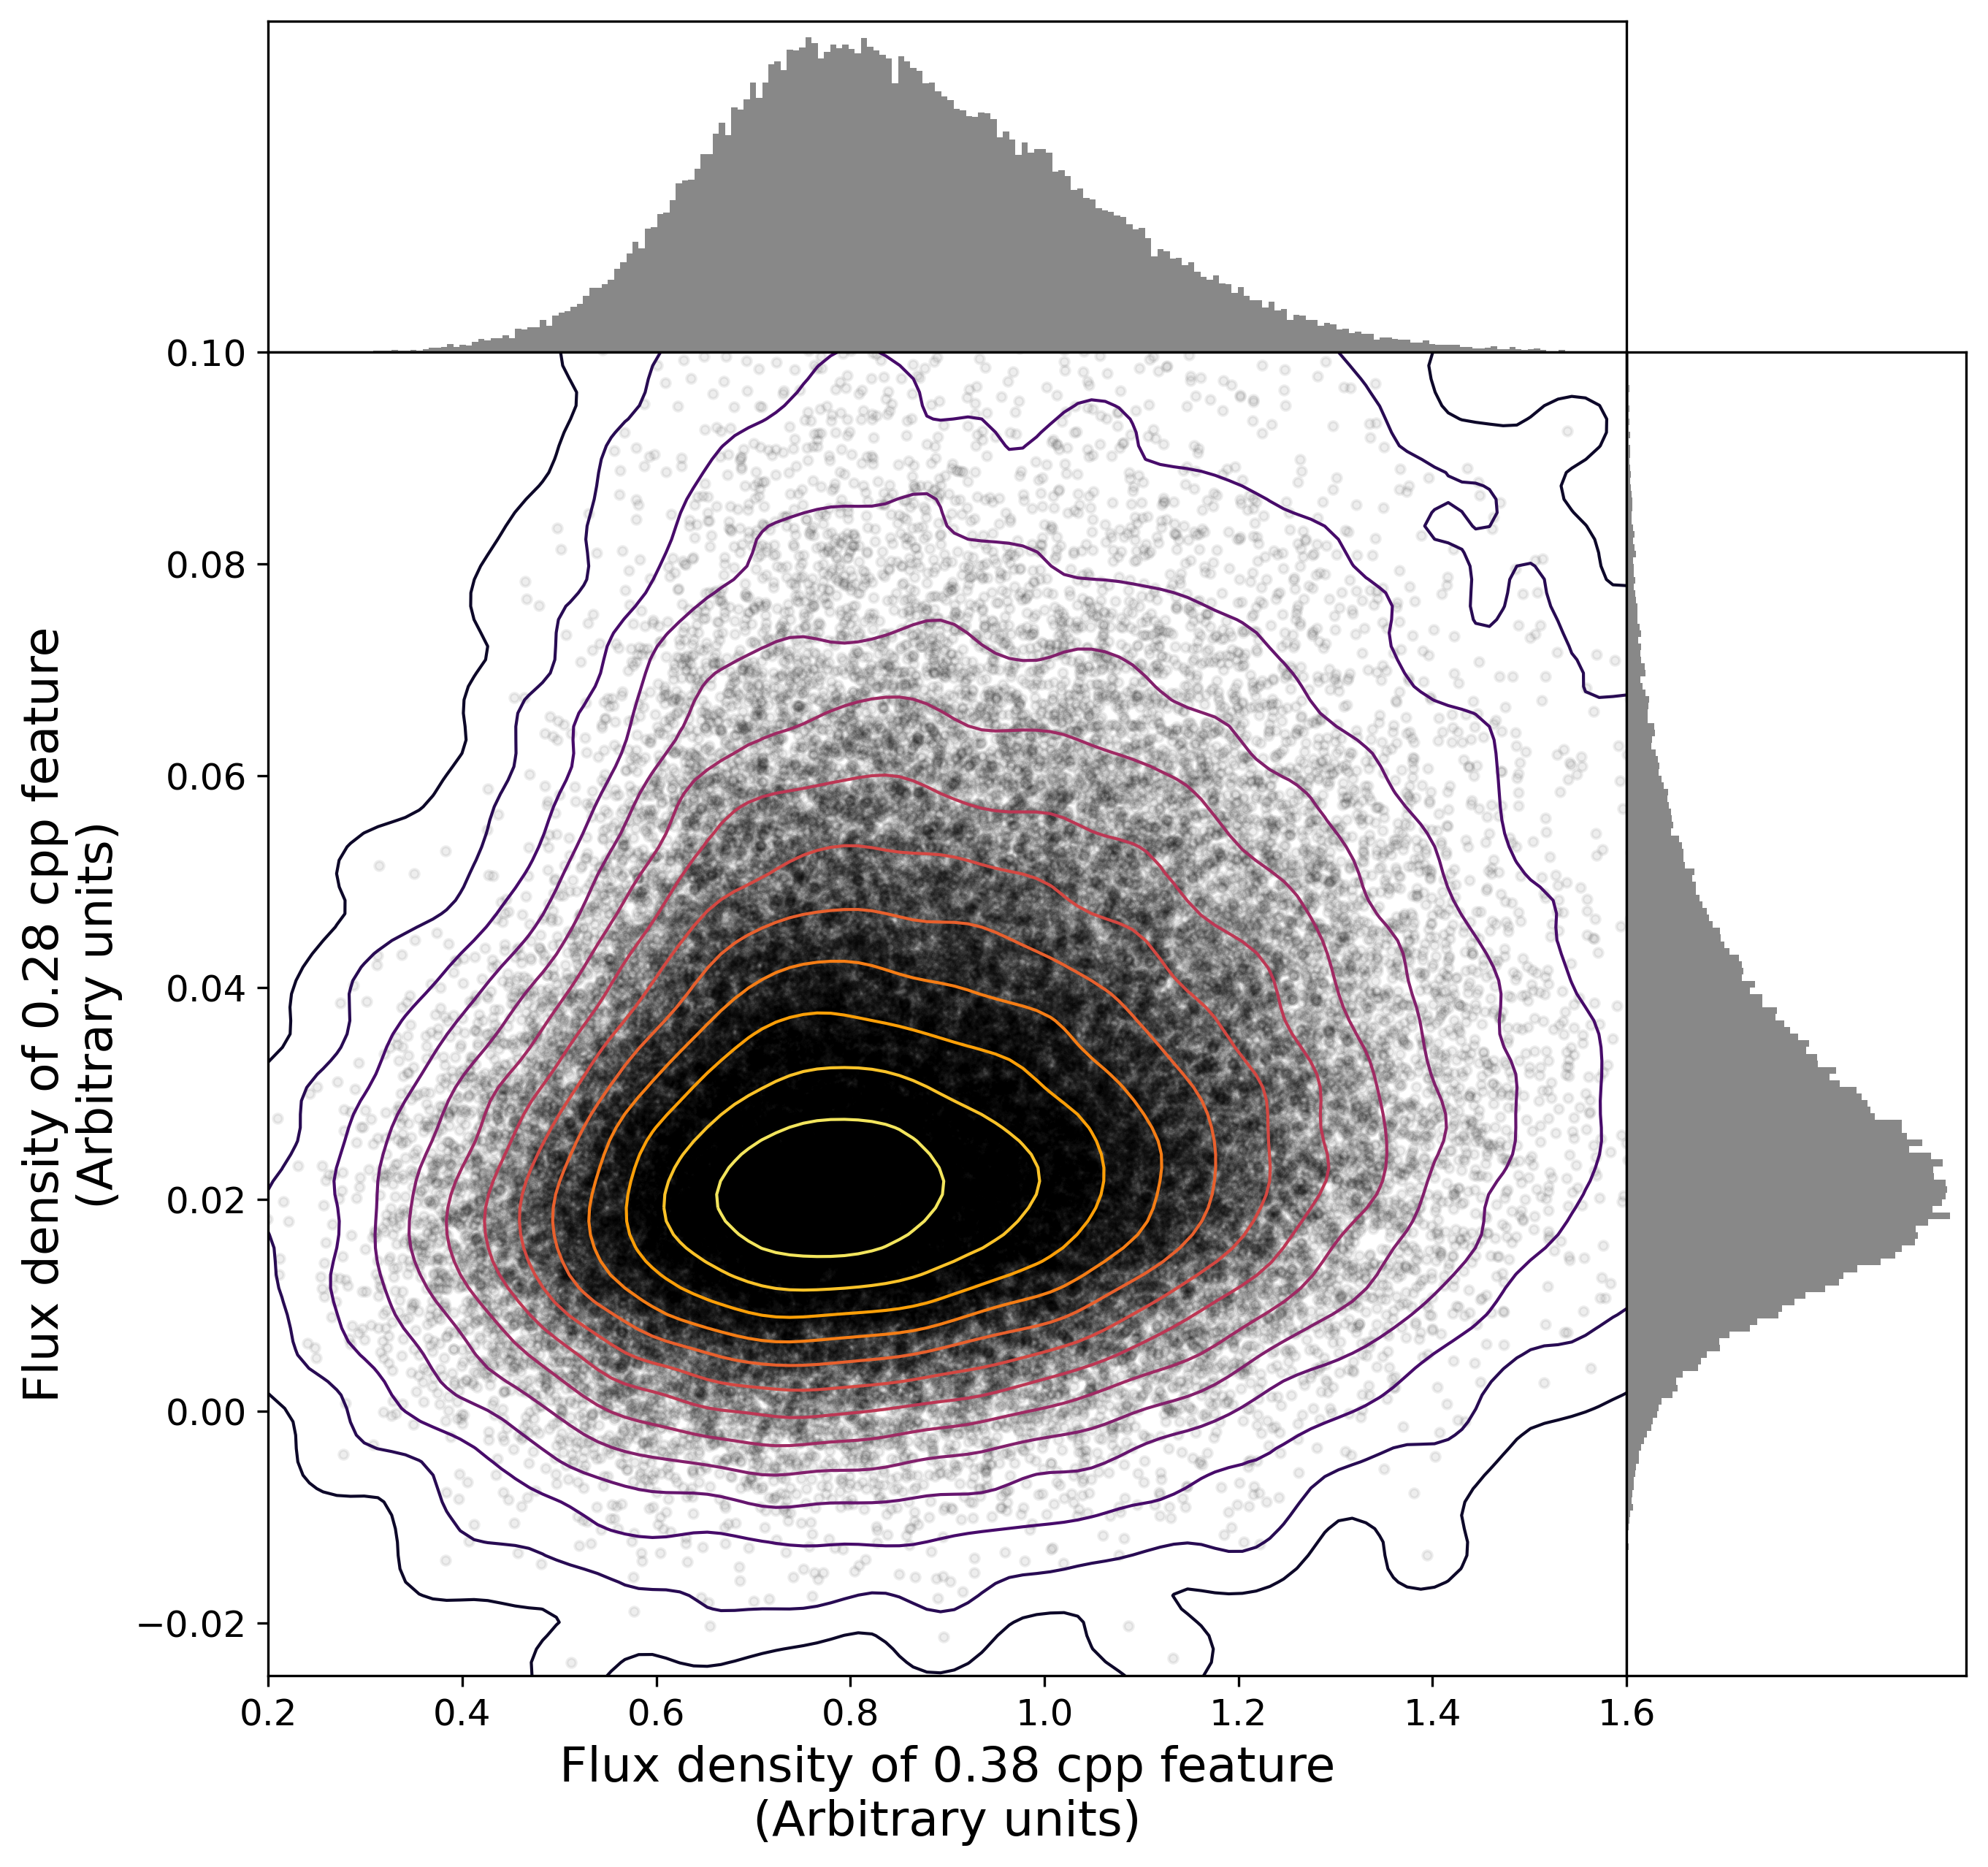
\includegraphics[width=0.7\textwidth]{Figures/J1518/energy_scatter.png}
        \caption[Profile component flux density comparison]{A scatter plot of the flux densities (in arbitrary units) integrated over the pulse longitude ranges corresponding to the modulation features at 0.38~cpp ($x$-axis) and 0.28~cpp ($y$-axis). The two quantities are shown in a scatter plot to highlight any correlation between them, after accounting for long-term variations in both components caused by the changing brightness of the pulsar over the course of the observation. The histograms in the side panels show the overall distribution for each pulse longitude range.}
        \label{fig: J1518 - energy scatter plots}
    \end{center}
\end{figure}

The flux densities integrated over the two pulse longitude ranges were measured using \texttt{penergy} in \textsc{psrsalsa} for all individual pulses, and these were then plotted against each other in a scatter plot. Long-term intensity variations caused by the changing elevation of the pulsar during the observation (and therefore its brightness) were removed by dividing the individual flux density measurements by the integrated flux density for the full profile using a running mean of 101 pulses. Figure~\ref{fig: J1518 - energy scatter plots} shows these results. The main panel shows the distribution in the relationship between the flux densities of the two regions, with the integrated flux density of the profile between $175.6\degr$ and $190.7\degr$ on the $x$-axis, and that of the region between $194.0\degr$ and $199.7\degr$ on the $y$-axis. Since the data is not flux-calibrated, these quantities are in non-physical units. The side panels show the overall integrated flux density distributions for the two regions. If mode-switching -- and hence an associated profile change where the relative intensity at the two pulse longitude regions is changing -- were occurring, we would expect bimodal structure with two distinct `islands' of points. No such feature can be seen in Figure~\ref{fig: J1518 - energy scatter plots}. If there is any bimodality in the flux density distribution, it is completely swamped by the pulse-to-pulse variability -- an attempt was made to account for this by summing every five pulses to smooth out short-term pulse shape changes associated with the periodic modulation. This had the effect that the distribution of points becomes a more symmetric and unimodal distribution. 















\subsection{Longitude-resolved auto- and cross-correlation functions}
\label{sec: J1518 - analysis - correlation} 

To further investigate the single-pulse modulation of PSR~J1518+4904, we also explore the longitude-resolved autocorrelation function (LRAC; \citealt{ESxx2003} -- an extension of the earlier integrated single-pulse autocorrelation function of \citealt{JAPx2001}) and the longitude-resolved cross-correlation function \citep[LRCC;][]{Pxxx1986}.


The LRAC, as implemented in \textsc{psrsalsa}, is computed by multiplying the Fourier transform for the flux densities of the pulse sequence at a given pulse longitude with its complex conjugate. The sequences of flux densities were `zero padded', i.e. extended by adding zeros, to at least double the length of the sequence to avoid effects related to the cyclic nature of Fourier transforms. In addition, extra zeros were added to make the length of the sequence a power of two for computational reasons. The zero padding has the result that there is a decrease of power with lag number, which is because of the finite average flux density of the pulsar. By assuming that the flux density is constant in the measured sequence of flux densities, this effect has been removed from the LRAC as shown in Fig.~\ref{fig: J1518 - LRAC}.

Although closely related to the LRAC, the LRCC as implemented in \textsc{psrsalsa} is computed somewhat differently. First of all, the mean pulse profile is subtracted from the individual pulses such that positive/negative correlations correspond to excess/reduced flux density. The cross correlation at lag $l$ is computed via
\begin{equation}
    \label{eq: J1518 - LRCC}
    \mathrm{LRCC}_{i,j}^l = \pm\sqrt{|\sum_nF_{i,n}F_{j,n+l}|},
\end{equation}
where $i$ and $j$ are the two pulse longitude bins which are compared (the flux densities of bin $j$ are lagged compared to those of bin $i$). The flux density at pulse number $n$ and bin number $i$ (or $j$) is $F_{i/j,n}$. Care is taken in the summation such that only pulse numbers for which both terms of the product $F_{i,n}F_{j,n+l}$ are within the observed sequence of pulses are used. The sign corresponds to the sign of the value obtained after summation.

The LRAC for the 2018-11-04 observation is shown in Fig.~\ref{fig: J1518 - LRAC}. As with the LRFS plots (Figs.~\ref{fig: J1518 - lrfs time evolution} and \ref{fig: J1518 - lrfs freq evolution}), two pulse longitudes are shown with different dynamic ranges. The left-hand panel shows the LRAC between $176\degr$ and $190\degr$ pulse longitude, whilst the right-hand panel extends from $192\degr$ to $212\degr$, and the vertical axis shows lags ranging from 1 to 20 (as expected, there is a large spike at zero lag which is not shown). The colour scale represents the correlation coefficients, where positive values are red and negative values are blue. The line plot in the side panels show the results of integration across the pulse longitude range. 
\begin{figure}
    \begin{center}
        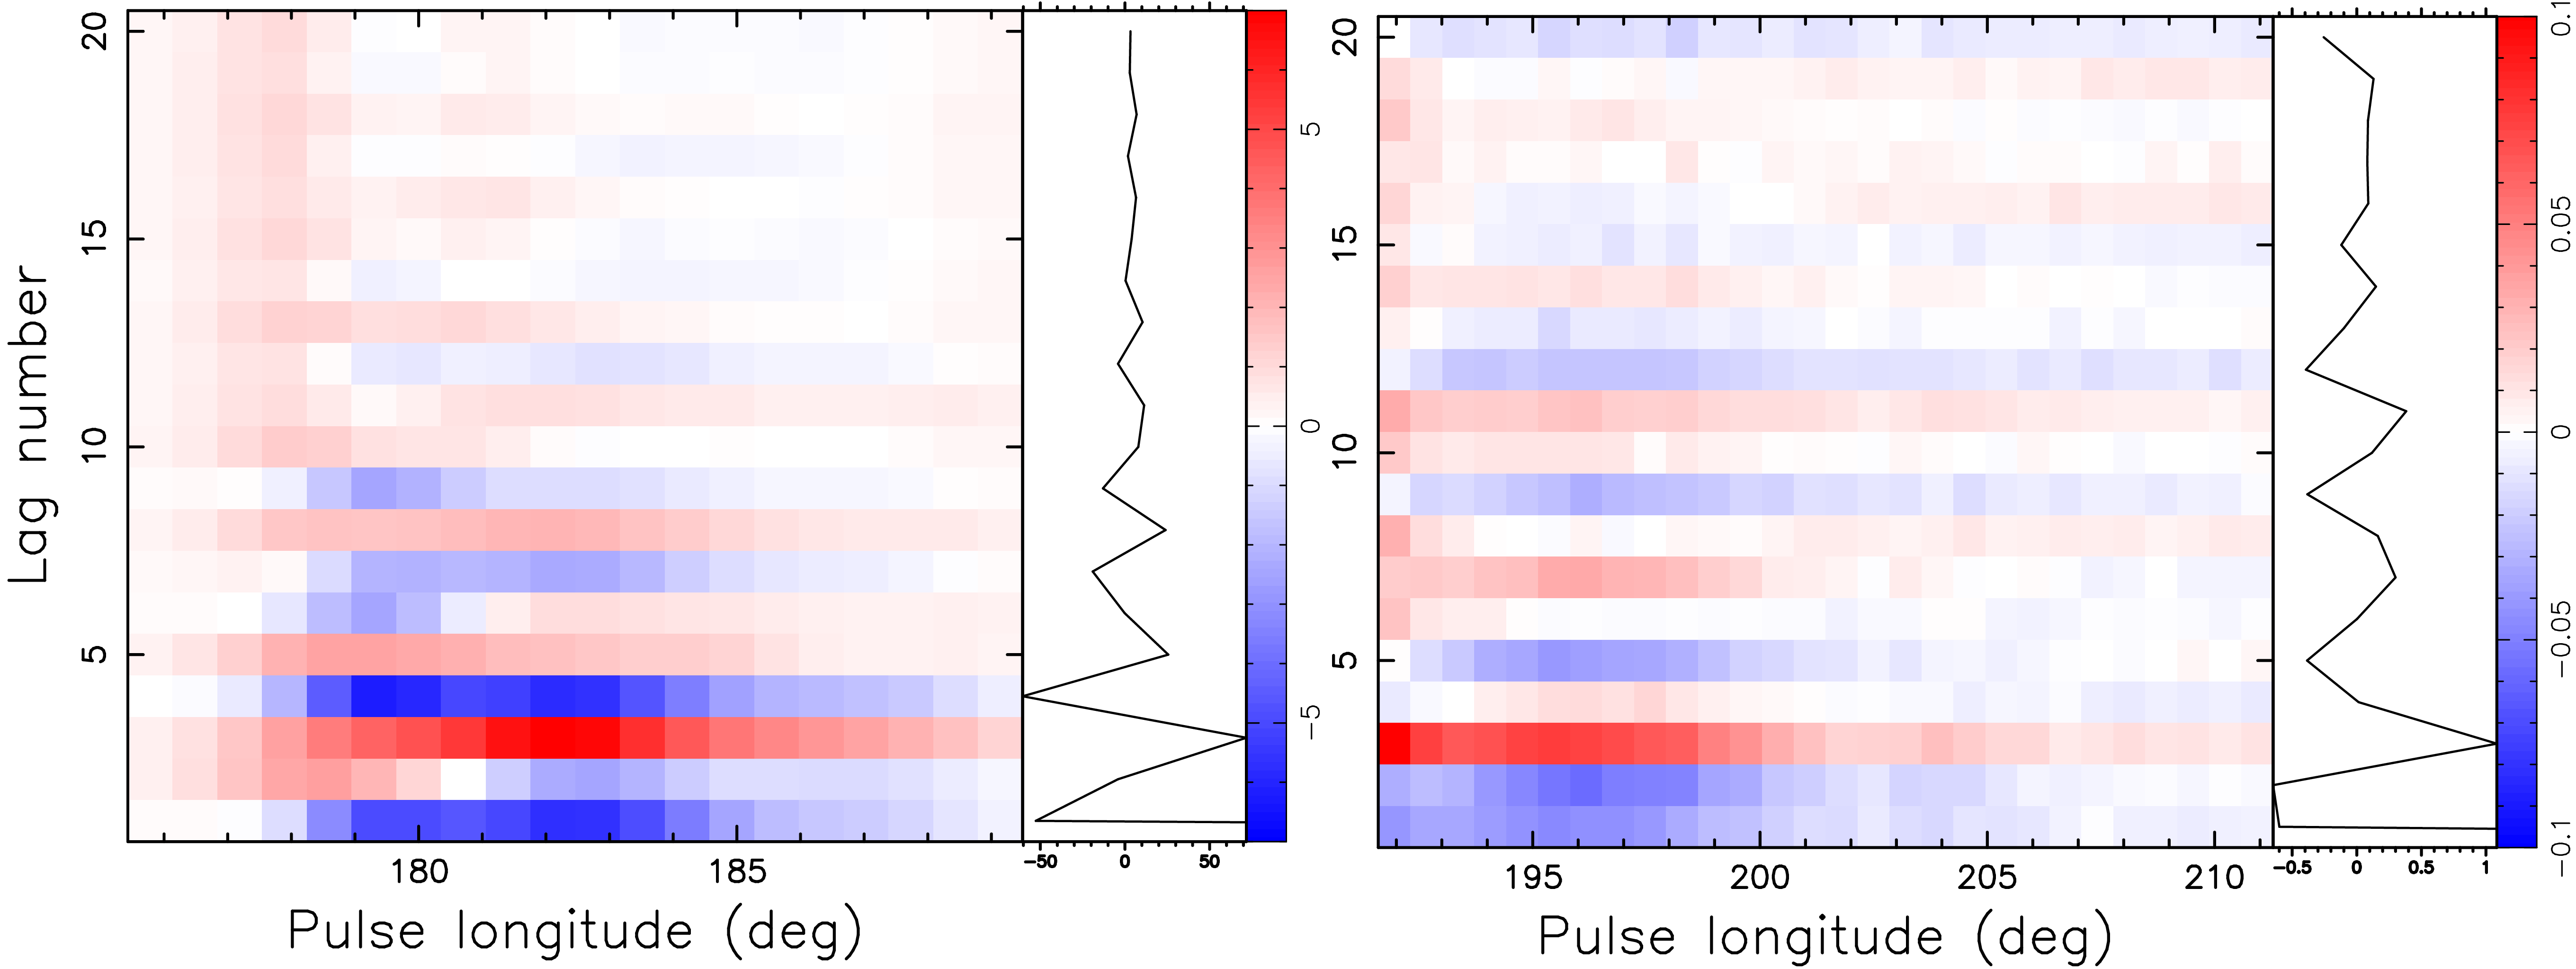
\includegraphics[width=\textwidth]{Figures/J1518/LRAC}
        \caption[The longitude-resolved autocorrelation spectrum]{The LRAC for lags 1--20, plotted between pulse longitudes $176\degr$ and $190\degr$ (left panel) and $192\degr$ and $212\degr$ (right panel). Positive values are shown in red, and negative values are blue. The side panels show the integrated spectrum across the window.}
        \label{fig: J1518 - LRAC}
    \end{center}
\end{figure}
The LRAC peaks at lag 3 for both longitude ranges, however the changing periodicity across the profile is evident. The gradual decrease in $P_3$ between profile components C1 and C2 is evident in the left-hand panel, revealed by the way the peak in the autocorrelation (with lag) changes. In the left-hand side panel the first maximum in the LRAC occurs between a lag of 2 and 3 pulses at the earlier longitudes, shifting to a lag of 3 pulses for most of the pulse longitude range. The minimum occurs at a lag of 4 pulses. In the second panel the first maximum again occurs at a lag of 3 pulses, with the following minimum at a lag of five pulses. This is consistent with the steady decrease in the modulation frequency observed with pulse longitude in the LRFS. In profile component C1 ($180\degr$), periodicities at both 0.07~cpp and 0.38~cpp are observed. Unfortunately the 0.07~cpp modulation is relatively weak, and its effect on the LRAC is too small to be recognised.

\begin{figure}
    \begin{center}
        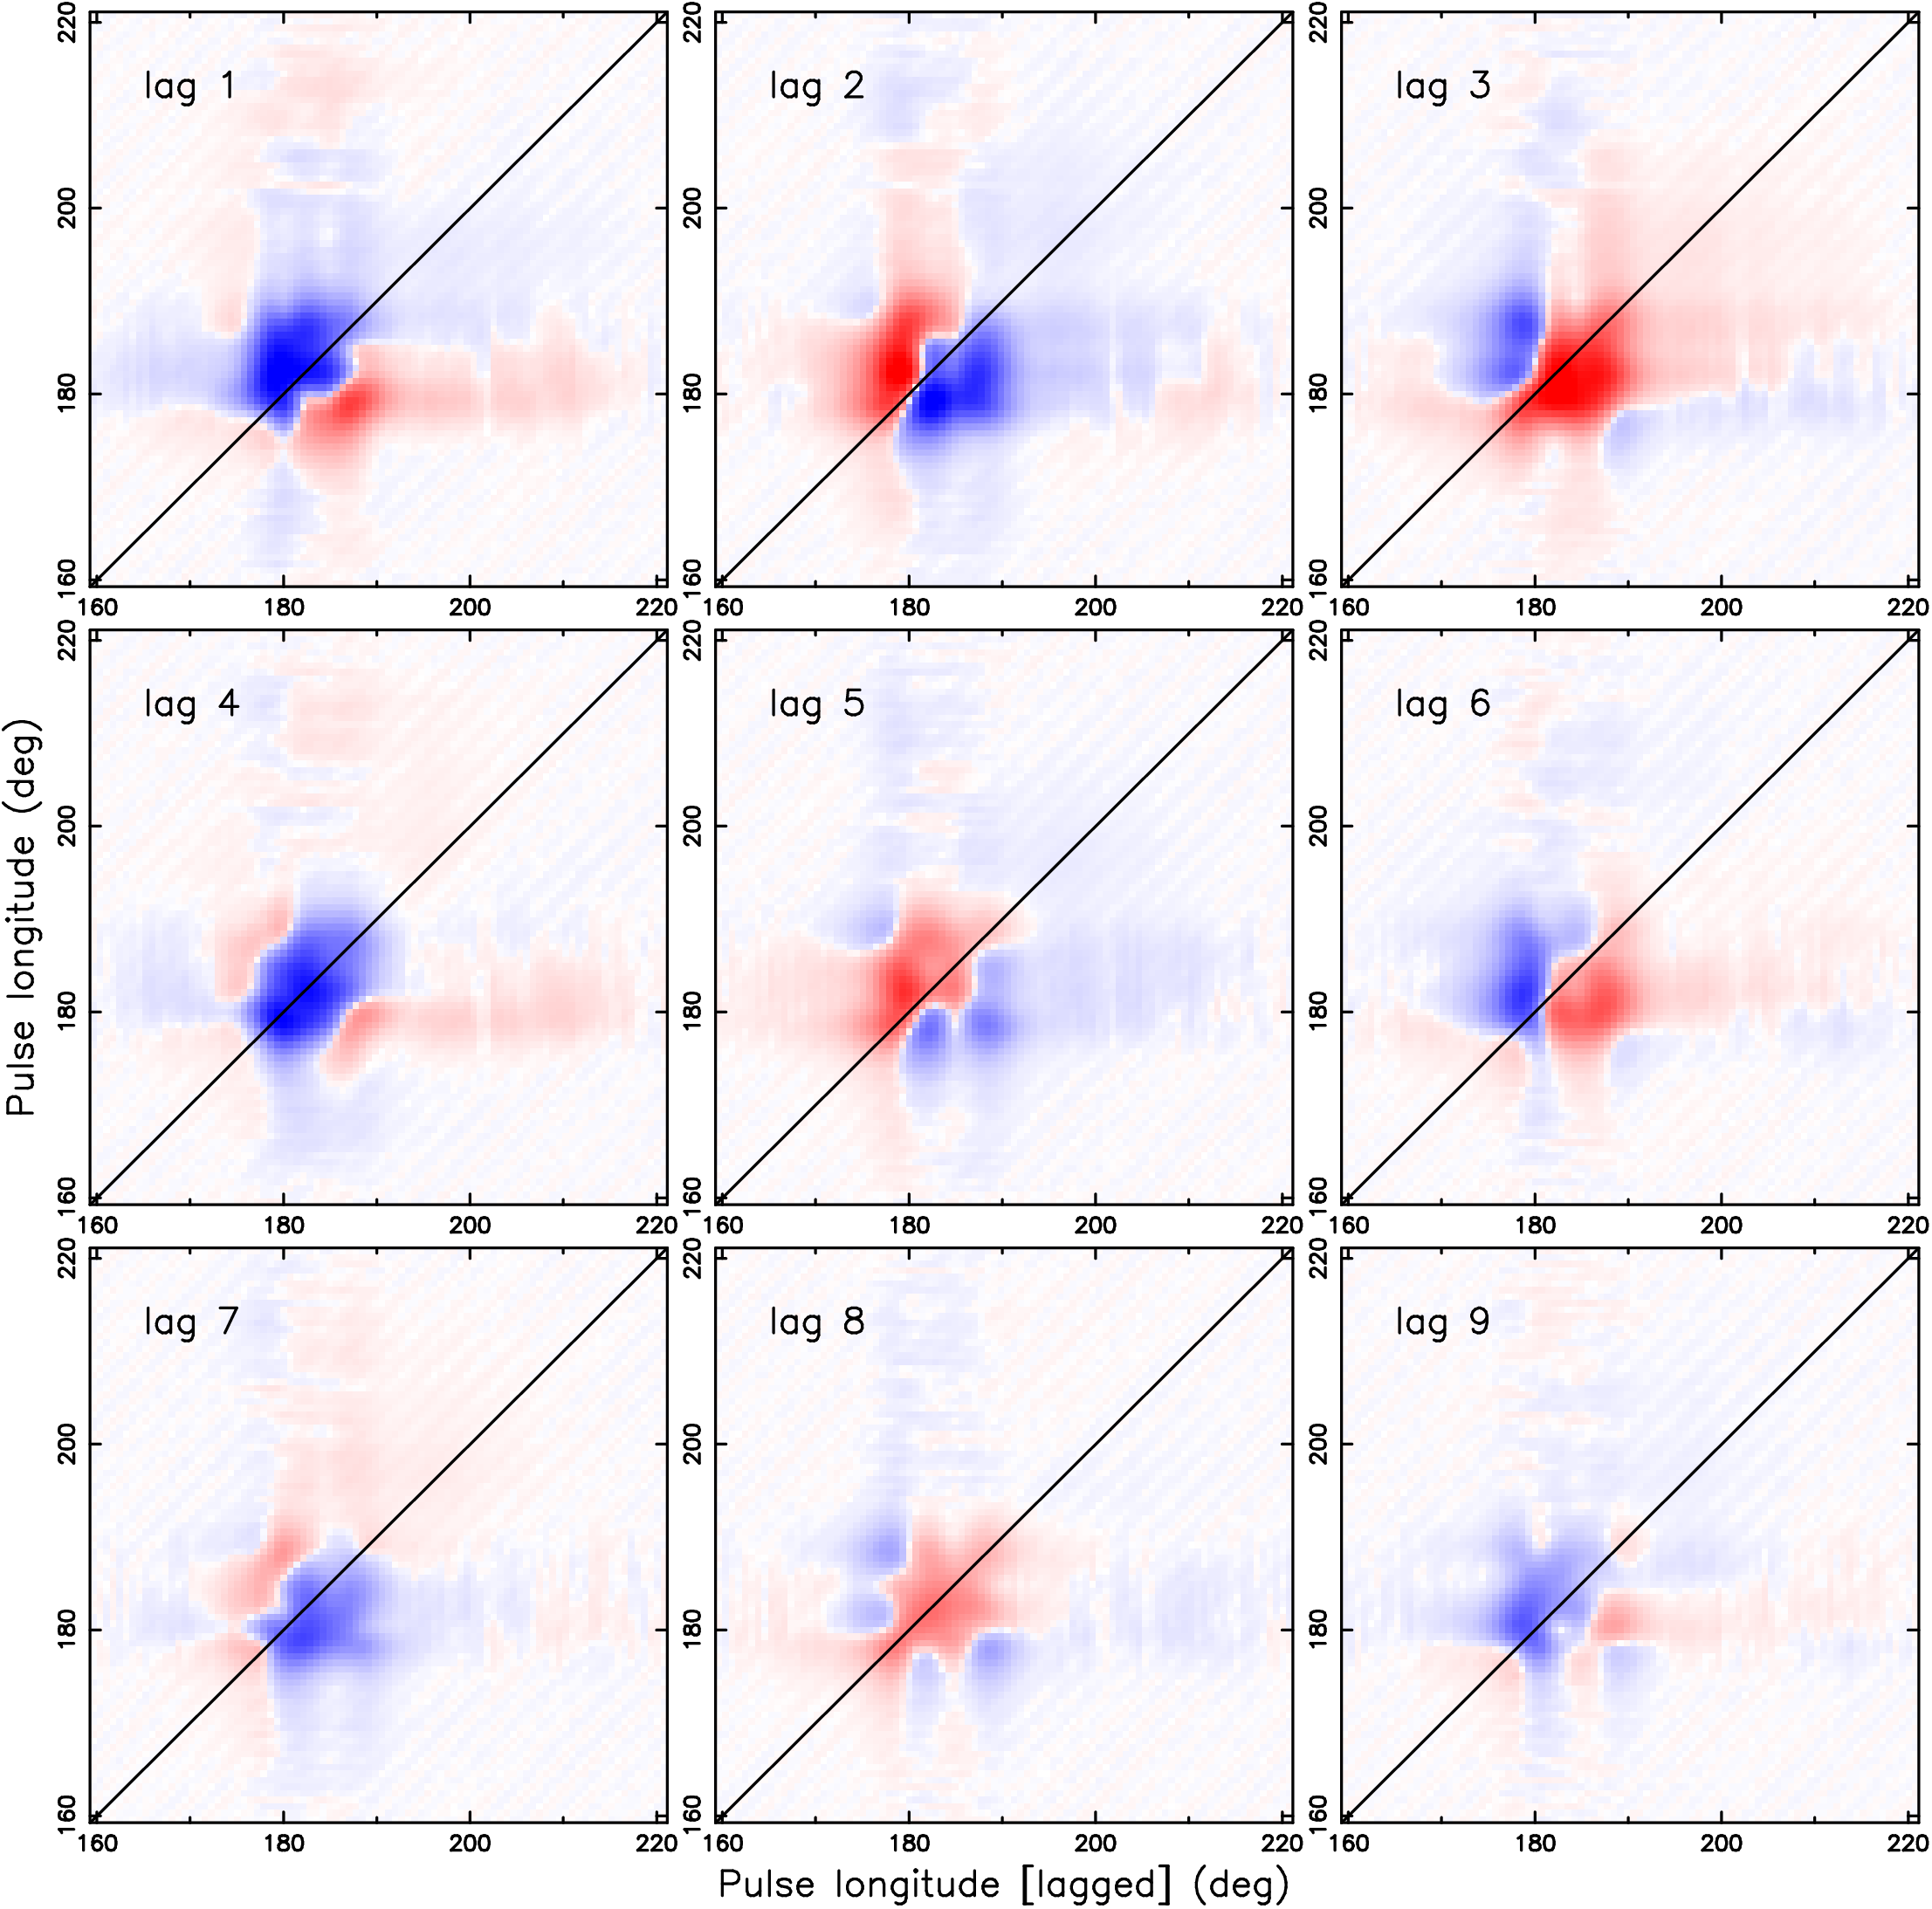
\includegraphics[width=1.0\textwidth]{Figures/J1518/LRCC}
        \caption[The longitude-resolved cross-correlation spectrum]{The LRCC is shown for lags 1--9 for the main profile between pulse longitudes $160\degr$ and $220\degr$. As with the LRAC, positive values are shown in red, and negative values are blue.  The diagonal black lines connect matching pulse longitude bins, so represent autocorrelations.}
        \label{fig: J1518 - LRCC}
    \end{center}
\end{figure}
The shift in modulation frequency with pulse longitude also manifests itself in the LRCC which is shown in Fig.~\ref{fig: J1518 - LRCC}, for lags ranging from 1 to 9. The diagonal black line in each panel connects bins with the same pulse longitude in the lagged and non-lagged pulse sequence, so represent the autocorrelation as seen in Fig.~\ref{fig: J1518 - LRAC}. As with the LRAC, the colour scale represents the correlation coefficients, with positive values denoted by red shading and negative values by blue. Correlations become anti-correlations and vice-versa as the lag number increases, corresponding to the rapid $0.38$~cpp modulation. The shifting position of the division between positive and negative correlations with pulse longitude implies drifting across the profile. As not all profile components fluctuate at the same frequency, this manifests itself as the emergence of more complex patterns in the later lags. These are fainter overall as the periodicities do not remain coherent over long timescales and so smear out any structure. Non-zero correlation coefficients are also faintly visible in a `$+$' structure in each panel, centred on the main profile components. It is unclear what the interpretation of this is, although it may be due to baseline variations on length scales slightly shorter than the pulse period (long-term variations were removed as described in Sec.~\ref{sec: J1518 - analysis - disjoint modes}).

There is some faint diagonal striping visible in the background of each panel which is the result of low-level, extremely rapid artificial baseline variations. These must be present throughout the observation as it is seen at all pulse longitudes. These are too weak to be a problem in any of the analysis presented in this work.




















\section{Discussion and conclusions}
\label{sec: J1518 - discussion}

\subsection{New profile components}
\label{sec: J1518 - discussion - new profile components}

The newly identified components in the integrated profile (C4 and C5, see Fig.~\ref{fig: J1518 - integrated profile}) greatly increase the fraction of the rotation period over which emission is detected (its `duty cycle'). The stronger of the two, C5 (at $\sim$275$\degr$), appears to be connected to the main component by a faint bridge of emission, which suggests that this is all part of the same emission region. If this is the case then the `main' profile width is extended to span at least $\sim$150$\degr$, or 0.42 pulse phase (estimated by measuring the region between components C1 and C5 where the pulsar emission is clearly visible over the background noise). The much weaker leading component C4 is consistent with being completely separate from the main profile, and could potentially be associated with emission from the opposite magnetic pole (i.e. an interpulse) as it is separated from the centre of the main profile by 165$\degr$, so roughly half a stellar rotation. If this is true, then that would suggest that PSR~J1518+4904 has a high magnetic inclination angle $\alpha$ that allows emission from both poles to be viewed. On the other hand, the main profile spanning C1--C3 and C5 is extremely wide, meaning that the emission beams themselves must be very wide (or the magnetic inclination angle $\alpha$ is extremely small). In the two-pole scenario, the narrow interpulse component C4 suggests the line-of-sight is only grazing the interpulse beam, meaning $\alpha$ may not be too large after all. Simultaneous observations of PSR~J1518+4904 covering a wide range of frequencies -- as performed for PSR~J0250+5854 in Chapter~\ref{chapt: J0250} -- would be very useful in exploring effects such as radius-to-frequency mapping that can be used to constrain the viewing geometry.

The new components do not appear to evolve much with frequency or time -- apart from the distinct change of the relative amplitude of component C2, which becomes brighter towards the top of the band relative to the other components (central panel of Fig.~\ref{fig: J1518 - profile frequency evolution}). This behaviour was seen by \citet{KLL+1999} in data taken with the 100~m Effelsberg telescope, and they noted that this component initially weakens between 370 and 610 MHz before increasing to become dominant at 1.8~GHz. In this work they also observe that the small, tertiary component of the main peak (around $210\degr$ pulse longitude in our figures) is stronger at low frequencies before fading out completely at 1.4~GHz. This is in contrast to their earlier observations using the same telescope \citep{KXL+1998} where this feature was discovered again at 1.4~GHz. The difference between these two data sets is that the later observations (between July 1997 and October 1998) were coherently dedispersed whereas the earlier observations (around April 1994) were not, although it is unclear why this should mean the tertiary profile component should disappear. Regardless, it is clearly present in the incoherently dedispersed FAST data, so this feature may vary in intensity over timescales of years. 










\subsection{Single-pulse modulation properties}
\label{sec: J1518 - discussion - funky P3}

The S2DFS (Fig.~\ref{fig: J1518 - S2DFS}) shows that the broadness of the modulation frequency peaks in the spectra is due to stochastic variation of the modulation frequency over unresolved timescales (i.e. smaller than 256 pulses). Stochastic variability is observed at all pulse longitudes.

The apparent change in $P_3$ as a function of pulse longitude is extremely unusual. The shift in $P_3$ with longitude is stable in time (Fig.~\ref{fig: J1518 - drifting P3 components}) and frequency (e.g. Fig.~\ref{fig: J1518 - lrfs freq evolution}). There is a trend where the 0.38~cpp component decreases slightly in fluctuation frequency and power between profile components C1 and C2 whilst the distribution of frequencies becomes broader. The 0.28~cpp periodicity that exists between C2 and C3 may be a continuation of this trend, although it seems to be a distinct feature. This more narrow feature is significantly offset from the main component at $P_3 = 2.659\pm0.008P_1$. We considered the idea that this is down to the presence of two distinct drift modes in PSR~J1518+4904, as seen for example in PSR~B0031$-$07 (Chapter~\ref{chapt: B0031}). The length of the FFT used in calculating the S2DFS (Fig.~\ref{fig: J1518 - S2DFS}) was 256 pulses, so if mode-switching were occurring on faster timescales it would not be resolved by this analysis.

It is also curious that the modulation feature at 0.28~cpp appears to be significantly weaker in the 2018-08-04 observation, without affecting the overall intensity, whilst the modulation features at 0.38~cpp and 0.07~cpp appear to be just as strong (see Fig.~\ref{fig: J1518 - lrfs time evolution}). It is highly unusual for pulsars to show time-dependent variation in modulation power (with the exception of mode changes). We hypothesised that this modulation feature could be present for only part of the observation, accounting for its overall weakness in the (time-averaged) LRFS; however, a S2DFS revealed that it is present throughout (but very weak). %\todo{Crispin non-thesis comment: I wonder if a this suggests that modulation is not caused by periodic brightening of the emission (such as the sparks of the carousel model) on a constant background, but rather both brightening and dimming about a mean value? Not sure how to test this.}

In the majority of pulsars, if periodic single-pulse fluctuations occur, they do so with the same periodicity across all profile components, although stochastic variation about the mean frequency is common. This has been demonstrated by \citet{Wxxx2007} who studied the LRFS and 2DFS for 187 pulsars. Some pulsars exhibit coherent drifting with very stable values of $P_3$, whereas the diffuse drifters more closely resemble what is seen for PSR~J1518+4904. There are a number of pulsars for which multiple distinct $P_3$ spectral features are seen, however these are attributed to mode changes, as many of them were previously known to do so. The 2DFS of PSR~B1929+10 at a wavelength of 21~cm was found to have two broad features with an opposite drift sense at different $P_3$ values, not unlike PSR~J1518+4904. These features were also observed by \citet{Bxxx1973} in the LRFS. A negative $P_2$ was detected for the short-period modulation feature, but the longer-period feature had a positive drift sense, and both were associated with the same profile components. The conclusion reached was that PSR~B1929+10 switches between drift modes with different $P_3$, and that the two modes have opposite drift directions. Seven pulsars were shown to have opposite drift directions in different components: PSRs B0450+55, B1540$-$06, B0525+21, B1839$-$04, B2020+28, B0329+54, and B1237+25. The $P_3$ values of these were the same however, and so their `bidrifting' may be attributed to non-circular carousels of sub-beams \citep[e.g.][]{QLZ+2004, Wxxx2016, WWxx2017, SLWM2020}.

Mode-changing behaviour is primarily associated with normal, non-recycled pulsars, with periods greater than 100 milliseconds. Nevertheless, total intensity and polarisation profile morphology changes have been observed in four recycled pulsars: PSRs J1022+1001, J1730$-$2304, B1821$-$24, and J2145$-$0750 \citep{KXC+1999}. The cause of the changes was determined to be intrinsic to the pulsars rather than due to propagation or hardware effects, and the authors stress that they are \textit{not} consistent with the mode-changing behaviour of normal pulsars -- for PSR J1022+1001, the profile changes occurred smoothly over hundreds of thousands of pulses. In normal pulsars, even those that exhibit mode changes, integration over $\sim$10,000 pulses are typically sufficient to produce a stable profile \citep{HMTx1975, RRxx1995}. Two of the four (PSRs J1022+1001 and J2145$-$0750) have an orbiting companion whereas the other two do not, implying that their profile changes are not necessarily due to them being in a binary system. Overall, the cause of the phenomenon could not be determined. 

Mode changing was robustly identified by \citet{MKMP2018} in PSR~B1957+20, a MSP with a period $P_1=1.6$~ms. This pulsar switches between two distinct modes on an average timescale of 1.7 seconds, the shortest mode-switching time observed to date. In units of pulse periods this timescale of $\sim 1000 P_1$ is not dissimilar to mode switching in normal pulsars though. PSR~B1957+20 has a narrow, single-component main pulse and a broad interpulse with two components. The main pulse is largely unaffected by the mode change, but the interpulse decreases in intensity, and its two components change in relative intensity. This change in relative intensity was the signature of mode switching we searched for in PSR~J1518+4904 by analysing the correlated changes in the flux density of the two regions of the profile that have different $P_3$ values in the LRFS (Fig.~\ref{fig: J1518 - energy scatter plots}). No bimodality could be seen in the distribution of either component separately, nor when combined in a scatter plot of both quantities.

As discussed extensively in Chapt.~\ref{chapt: B0031}, the carousel model is the most well-known and developed model of for sub-pulse drift. It can explain many of the commonly observed features of subpulse drifting, by modelling the subpulses as a pattern of sub-beams that circulates around the magnetic axis \citep[e.g.][]{RSxx1975, DRxx1999, GSxx2000, GMGx2003}. The circulation of the carousel is the result of an $\mathbf{E} \times \mathbf{B}$ drift \citep{RSxx1975}. If drifting occurs at varying altitudes in the magnetosphere where the fields are different, this could potentially explain slight shifts in $P_3$ over time. However, this is distinctly different from the standard picture where the drift arises because of $\mathbf{E} \times \mathbf{B}$ in the polar gap near the surface, which causes the sites (`sparks') of particle injection into the magnetosphere to drift, resulting in a corresponding drift of the radio emission generated at higher altitudes. %\todo{MELROSE PAPER ABOUT MAGNETOSPHERE-WIDE DRIFT - DIFFERENTIAL ROTATION?}

Even without invoking differences in the circulation period of the carousel $P_4$, discrete changes in $P_3$ could arise if the number of sub-beams can change. The alias effect which occurs for fast circulation (see for example Appendix~\ref{app: geometry derivations}) can explain subsequent reversals in the drift direction \citep[e.g.][]{Wxxx2007}. Simultaneous drifting at two different $P_3$ values in different profile components could hypothetically occur when nested carousels are considered, as is the case in the core-cone model \citep[e.g.][]{Rxxx1983a, Kxxx1994, GGxx2003}. If the nested carousels either circulate with different periods or have a different number of sub-beams, different $P_3$ values are predicted to be observed simultaneously. However, the question is why this should be the case for PSR~J1518+4904 and not frequently observed in the broader population? Furthermore, in such a model we might expect some degree of symmetry about the fiducial plane (see Chapter~\ref{chapt: B0031}) in terms of the emission properties (a symmetric pattern of $P_3$ values as a function of pulse longitude is implied for example). Such symmetry is entirely absent in PSR~J1518+4904. 

An alternative mode for single-pulse modulation is non-radial oscillations of neutron stars. Originally proposed as the source of radio emission in pulsars \citep{Rxxx1968}, these were later suggested as the possible origin of drifting subpulses \citep{DCxx1968}, revised by \citet{CRxx2004}. Although they provide a natural explanation for phenomena such as discontinuities in subpulse phase (similar to the feature observed in PSR~J1926$-$0652; Chapter~\ref{chapt: J1926}), nulling, and mode changing, fine tuning is required to explain the longitude-dependence of $P_2$ commonly seen in driftbands.  Although a drift direction reversal can in principle be explained as a change in the beat frequency between oscillation and stellar rotation, the model struggles to explain pulsars that exhibit modulation with opposite drift directions in different components simultaneously.

Whilst discrete changes in $P_3$ as a function of longitude can hypothetically be attributed to unresolved mode changes (although we have found no evidence for any), the apparent smooth change between profile components C1 and C2 (Fig.~\ref{fig: J1518 - drifting P3 components}) cannot be explained. It cannot occur under the carousel model as it would require a smooth variation of circulation rate at different locations. If differential rotation is possible in pulsar magnetospheres it is unclear how any sub-beam-like structure can be maintained as a function of magnetic azimuth. Any distinct pattern would rapidly be smeared out, so a mechanism should exist to regenerate the pattern in order for circulation to be observable as drifting subpulses. If that is the case, it is unclear why the same number of beamlets are being regenerated each time, and hence why the same periodicities are being observed over extended periods.


In conclusion, we have discovered curious modulation properties for PSR~J1518+4904. In particular, the longitude-dependent modulation observed in part of the profile is unique in the pulsar population. This finding presents some serious challenges for existing models of pulsar emission and how they can explain the observed pulse-to-pulse variability in radio pulsars. The work in this chapter has shown that this pulsar merits further observations with FAST, which is currently fully commissioned and operational with good polarisation capabilities (see Chapter~\ref{chapt: J0250}), and a proposal to do so has been submitted. These observations could establish with certainty whether the observed modulation effects are indeed fully associated with changes in Stokes $I$, or if some of the variability arises because of periodic changes in polarisation. This could add an additional layer of complexity to an already problematic-to-interpret dataset.



\chapter[A broadband radio study of PSR~J0250+5854]{A broadband radio study of PSR~J0250+5854: the slowest-spinning radio pulsar known}
\label{chapt: J0250}

Here I present simultaneous observations of the most slowly rotating known radio pulsar, PSR~J0250+5854, (period $P_1 = 23.5$~s) with FAST, two LOFAR international stations (UK608 at Chilbolton and DE601 at Effelsberg), and NenuFAR. The detections of this pulsar at 1250~MHz (FAST) and 57~MHz (NenuFAR) are the highest- and lowest-frequency published detections respectively to date, increasing the spectral coverage of this object by a factor of five. While PSR~J0250+5854 is slow, its continued radio emission beyond the canonical death line can be explained by, for example, the partially screened gap model. A flux density of $4\pm2$~$\upmu$Jy was measured at 1250~MHz giving an exceptionally steep spectral index of $-3.5^{+0.2}_{-1.5}$, with a turnover below $\sim95$~MHz. In conjunction with previous observations of this pulsar with the GBT and LOFAR Core, I show that the intrinsic profile width increases towards higher frequencies, contrary to the predictions of conventional radius-to-frequency mapping. This implies that the beam filling fraction is lower at low frequency. I use polarimetric data from FAST and LOFAR Core to constrain the emission geometry of PSR~J0250+5854, leading to the conclusion that its polar cap radio emission is produced at an absolute height of several hundreds of kilometres, similar to the other rotation-powered non-recycled pulsars, supporting the argument that emission height is relatively constant across the population. Finally, I draw a comparison between PSR~J0250+5854 and the other slow rotation-powered pulsars,  and contrast these with the radio-detected magnetars. I conclude that although they have similar spin periods, the magnetars have intrinsically wider radio beams than the slow rotation-powered pulsars. Consequently, the lower beaming fraction of the latter is what makes objects such as PSR~J0250+5854 so scarce. This work is under review for publication \citep{AWB+2021}.
% We present simultaneous observations of the most slowly-rotating known radio pulsar PSR~J0250+5854 (period $P=23.5$~s) with FAST, two LOFAR international stations (UK608 at Chilbolton and DE601 at Effelsberg), and NenuFAR. The detections with FAST at 1250~MHz and NenuFAR at 57~MHz are the highest- and lowest-frequency published detections respectively to date, and represent a five-fold increase in the spectral coverage of this object. We measure a flux density of $4\pm2$~$\upmu$Jy at 1250~MHz and an exceptionally steep spectral index of $-3.5^{+0.2}_{-1.5}$, with a turnover below $\sim$95~MHz. In conjunction with observations of this pulsar with the GBT and the LOFAR Core, I have shown that the intrinsic profile width increases towards higher frequencies, contrary to the predictions of conventional radius-to-frequency mapping. We used polarimetric data from FAST and the LOFAR Core to constrain the emission geometry of PSR~J0250+5854. This leads to the conclusion that its polar cap radio emission is produced at an absolute height of several hundreds of kilometres, similar to other rotation-powered pulsars and suggesting that it is relatively constant across the population. Finally, the results for PSR~J0250+5854, and those of other slowly-spinning rotation-powered pulsars are contrasted with those of the radio-detected magnetars. We conclude that magnetars have intrinsically wider radio beams than the slow rotation-powered pulsars, and that consequently the lower beaming fraction of the latter is what makes objects such as PSR~J0250+5854 so scarce.





\section{Introduction}
\label{sec: J0250 - introduction}

Pulsars are rapidly rotating, highly magnetised neutron stars; however, some pulsars rotate significantly less rapidly than others. In this chapter I discuss observations of PSR~J0250+5854, a radio pulsar with a period $P_1=23.5$~s discovered by \citet{TBC+2018} in the Low Frequency Array (LOFAR) Tied-Array All-Sky Survey \citep[LOTAAS;][]{SCB+2019}. It was detected with the LOFAR High Band Antenna array between 110--190~MHz, and with the Green Bank Telescope (GBT) between 300--400~MHz. It is the longest-period radio pulsar discovered to date, more than twice the period of the second slowest-spinning \citep[PSR~J2251$-$3711 at $P_1 = 12.1$~s;][]{MKE+2020} and almost three times slower than the well-studied 8.5~s pulsar PSR~J2144$-$3933 \citep{YMJx1999}. %Finding such a slow pulsar is rare, which may be explained by the fact that slower pulsars lose their ability to create electron-positron pairs and accelerate them sufficiently to produce the detectable coherent radio emission \citep{Sxxx1971}, and by their lower beaming fractions which make it less likely that they are visible to an Earthbound observer. In addition, there are practical issues with detecting slow pulsars due to selection effects making them significantly harder to identify in pulsar survey data if only a small number of pulses are present. The presence of red noise in periodicity searches further hinders their identification \citep[e.g.][]{LBH+2015,HKRx2017}.
Finding such a slow pulsar is rare, which may be explained by the fact that slower pulsars have lower beaming fractions which make it less likely that they are visible to an earthbound observer, and practical issues due to selection effects, making them significantly harder to identify in pulsar survey data (if only a small number of pulses are present). The presence of red noise in periodicity searches further hinders their identification \citep[e.g.][]{LBH+2015,HKRx2017}.


Furthermore, older, slower pulsars lose their ability to create electron-positron pairs and accelerate them sufficiently to produce the detectable coherent radio emission \citep{Sxxx1971}. Therefore, models for radio emission can be constrained by finding the slowest pulsars that are still active. As discussed in \citet{TBC+2018}, PSR~J0250+5854 occupies a relatively empty part of the $P$-$\dot{P}$ diagram, beyond the `death valley' as defined by \citet{CRxx1993} and the vacuum-gap curvature radiation death line proposed by \citet{ZHMx2000}, but it is consistent with the partially screened gap model \citep[e.g.][]{Sxxx2013}. Although PSR~J2144$-$3933 rotates almost three times faster, its much smaller spin-down rate $\dot{P} = 4.96\times10^{-16}$~s~s$^{-1}$ makes it more constraining for radio emission models \citep{MBMA2020}.


The extreme period of PSR~J0250+5854 places it in the company of the magnetars which have periods of 2--12~s \citep{OKxx2014}, but its spin-down rate of $\dot{P}~=~2.72\times10^{-14}$~s~s$^{-1}$ is around a thousand times smaller than those of the magnetars.  It also lies close to the parameter space inhabited by the population of X-ray Dim Isolated Neutron Stars (XDINSs). Of the seven brightest XDINSs, five have high magnetic dipole fields of the order of $10^{13}$--$10^{14}$~G which may mean they are related to magnetars \citep[][see Sec~\ref{sec: intro - general intro - pulsar population}]{Hxxx2007, KKxx2007}. These objects are detected only as soft thermal X-ray sources without radio counterparts. However, to date PSR~J0250+5854 remains undetected in X-rays, despite a dedicated \textit{Swift} X-Ray Telescope observation, which makes it difficult to confirm a connection between it and XDINS (see \citealt{TBC+2018} for details). Similarly, PSR~J0250+5854 has not shown any magnetar-like behaviour such as bursts, or any large radio variability as of yet.


This work details the first detection of PSR~J0250+5854 at frequencies between 1 and 1.5~GHz using the Five-hundred-metre Aperture Spherical radio Telescope (FAST), along with simultaneous observations with the UK608 and DE601 LOFAR international stations, and NenuFAR (New Extension in Nan\c{c}ay Upgrading loFAR). The NenuFAR detection at 57~MHz is the lowest-frequency detection of PSR~J0250+5854 published to date, and the FAST detection the highest, resulting in an extension by a factor of $\sim$5 in spectral coverage of this unique source in the radio domain. Upon its discovery \citet{TBC+2018} were able to detect PSR~J0250+5854 over the frequency range between 120 and 350~MHz, and fitted a spectral index of $-2.6\pm0.5$. However, with no detection of the pulsar at around 1500~MHz using the Lovell and Nan\c{c}ay radio telescopes, nor a detection with the core LOFAR Low Band Antenna stations (at 55~MHz), uncertainty remained over the broadband shape of the radio spectrum. 


A key part of understanding the pulsar emission mechanism lies in studying their radio frequency evolution. This is particularly relevant for pulsars such as PSR~J0250+5854 which are on the cusp of the death line. Multi-wavelength observations can provide information on features including the spectral index (how the flux of the pulsar changes with frequency), and changes in the shape and polarisation properties of the radio beam.

Measurements of pulsar radio spectra from a large population began with \citet{Sxxx1973}, \citet{MMxx1980} and \citet{IKMS1981} using frequencies around and below 100~MHz. Most pulsars were found to have steep spectra which could be modelled with a simple power law $S_\nu \propto \nu^k$, where $S_\nu$ is the mean flux density at some frequency $\nu$ and $k$ is the spectral index. For some pulsars deviations from this relation were identified in the form of a turn-over at low frequencies which can be attributed to absorption mechanisms, whilst others show a cut-off at high frequencies due to a steepening or break in the spectrum \citep{Sxxx1973}. Two recent studies of radio pulsar spectral indices have been performed by \citet{BKK+2016} and \citet{JSK+2018}. \citet{BKK+2016} studied the spectra of 165 non-recycled pulsars in the Northern sky with LOFAR, and found that 124 were best fitted by the simple power-law model, whilst the remaining 41 were fitted with a broken power law. They found a mean spectral index of $k = -1.4$. Similarly, \citet{JSK+2018} studied 441 pulsars and found that 79~per~cent obeyed a simple power-law relation. The spread of spectral indices is described by a shifted log-normal distribution with a weighted mean of $-1.60\pm0.03$ and a standard deviation of 0.54, and this study covered centre frequencies of 728, 1382, and 3100~MHz using the Parkes radio telescope.

With its period of 23.5~s, PSR~J0250+5854 has an extremely large light-cylinder (with a radius $R_\mathrm{LC} = cP_1/2\pi =  1.123\times10^{6}$~km, where $c$ is the speed of light), and hence a tiny polar cap which connects to the open-field-line region (see Sec.~\ref{sec: intro - general intro}). The diameter of the polar cap is $D_\mathrm{PC} \approx 2R\sqrt{R/R_\mathrm{LC}} \approx~60$~m, where $R = 10$~km is the canonical neutron star radius \citep[e.g.][]{Sxxx1971}. By comparison, a pulsar with a period $P_1 = 0.5$~s would have $D_\mathrm{PC} \approx 410$~m. This implies that for typical emission heights of hundreds of kilometres, the radio beam of PSR~J0250+5854, and hence the duty cycle of its radio pulse, can be expected to be very narrow. Indeed \citet{TBC+2018} reported a pulse width of only $\sim$1$\degr$ at 129, 168, and 350~MHz. 

The shapes of pulse profiles after correcting for propagation effects (see Sec.~\ref{sec: intro - observation processing - ISM effects}) are in general observed to be frequency-dependent. Often, the profile width is seen to decrease with increasing frequency, which suggests that higher-frequency emission is produced lower in the magnetosphere. This correlation is known as radius-to-frequency mapping (RFM hereafter), and was first theorised by \citet{RSxx1975} who related the emission height to the local plasma frequency in the magnetosphere. The electron density (and hence plasma frequency) is expected to decrease with increasing altitude ($\rho \propto r^{-3}$), thereby predicting that the radio beam expands with decreasing frequency. However, a number of pulsars have been found to deviate from this relation \citep[e.g.][]{Txxx1991, CWxx2014,PHS+2016} -- this suggests the same set of magnetic field lines are not necessarily active at all frequencies (or emission heights), resulting in the appearance and disappearance of profile components with observing frequency \citep[e.g.][]{Cxxx1978, MRxx2002}. This can obfuscate the geometrical interpretation of measured profile widths, and is discussed further in Sec.~\ref{sec: J0250 - discussion - profile width}. Radio polarisation data can help in disentangling these effects, which is further explored for PSR~J0250+5854 in Sec.~\ref{sec: J0250 - analysis - polarisation and geometry}, although degeneracies often remain \citep[e.g.][]{KJW+2010}.

The structure of this chapter is as follows. In Sec.~\ref{sec: J0250 - observations} the new observations are described, followed by a brief explanation of the radio-frequency interference (RFI) excision techniques used. The analysis of the data described in Sec.~\ref{sec: J0250 - analysis} is divided into three parts: pulse profile evolution with frequency, polarisation properties, and the spectral shape of the pulsar flux density. These results are then discussed in a broader context in Sec.\ref{sec: J0250 - discussion}, and the conclusions are summarised in Sec.~\ref{sec: J0250 - conclusions}.




















\section{Observations}
\label{sec: J0250 - observations}

As part of a shared-risk proposal, PSR~J0250+5854 was observed on 22 May 2019 with FAST, a facility built and operated by the National Astronomical Observatories, Chinese Academy of Sciences \citep{NLJ+2011,LWQ+2018}. The central beam of the 19-beam receiver operating between 1 and 1.5~GHz \citep{JTH+2020} was used. At the time of these observations FAST was commissioned, and full polarisation information is available -- the issues detailed in Chapters~\ref{chapt: J1926} and \ref{chapt: J1518} have now been resolved. Two LOFAR international stations -- UK608 (United Kingdom) and DE601 (Germany) --- and NenuFAR (France) provided overlapping observations. Chilbolton is home to the UK LOFAR station UK608, formally known as the Rawlings Array, and the DE601 station is located at Effelsberg\footnote{DE601 was operated as part of the German Long Wavelength (GLOW) consortium at the time of these observations, in a coherently dedispersed folding mode.}. They each consist of two sub-arrays: the High Band Antenna (HBA; 110--240~MHz) and Low Band Antenna (LBA; 10--90~MHz) \citep{HWG+2013,SHA+2011}, although only the HBA were used in this project and the bandwidth was limited to 110--190~MHz. At the time of these observations, NenuFAR consisted of 52 groups of 19 dual-polarised antennas, operating between 10 and 85~MHz \citep{ZDT+2020}. It is located alongside and extends the capabilities of the Nan\c{c}ay LOFAR station (FR606). Table \ref{tab: J0250 - observations} gives a summary of the overlapping observations conducted. The LOFAR international stations observed PSR~J0250+5854 over the full duration of the FAST observations, and in the case of NenuFAR significantly longer.

Prior to observing PSR~J0250+5854, FAST performed a $\sim$15-minute observation of a well-known, bright pulsar PSR~J0139+5814 to validate the set-up of the observing system. A noise diode signal was injected into the FAST multibeam receiver to facilitate polarisation calibration (see Sec.~\ref{sec: intro - observation processing - polarisation calibration}). PSR~J0250+5854 was observed for two consecutive hours, interspersed with noise diode observations. Finally, the BL Lacertae object J0303+472 \citep{VVxx2006} was observed for purposes of flux calibration (see Sec.~\ref{sec: intro - observation processing - flux calibration}) -- this source was chosen due to its proximity to PSR~J0250+5854.

All data were folded and de-dispersed with \textsc{dspsr} \citep{SBxx2011} using the ephemeris and dispersion measure (DM) reported in \citet{TBC+2018} to form a pulse sequence. De-dispersion was done coherently for the DE601, UK608, and NenuFAR data, and incoherently for the FAST data. Flux and polarisation calibration were done using the \texttt{pac} program in \textsc{psrchive} \citep{SMJR2010}. Further processing made use of \textsc{psrsalsa} \citep{Wxxx2016} and is described later in this chapter.

Although not part of the simultaneous observations, this project also made use of an observation of PSR~J0250+5854 using the LOFAR Core stations \citep{HWG+2013} conducted on 28 October 2017. This was part of a run of observations conducted by \citet{TBC+2018}, but is a different data set to the profiles shown in that paper. This LOFAR Core observation was similarly processed with \textsc{psrchive}.

\begin{landscape} % Maybe not landscape, but needs tweaking!
    \begin{table}
        \centering
        \caption[Summary of the simultaneous observations of PSR~J0250+5854]{Observation properties of the analysed observations. There is a full overlap of the data for the period during which FAST was recording data for PSR~J0250+5854 on 22 May 2019 (these observations are denoted with a *). `Resolution' is the number of samples (pulse longitude `bins') per pulse period. The GBT and LOFAR Core observations were performed earlier, on 2017-10-25 and 2017-10-28 respectively.}
        \label{tab: J0250 - observations}
        \begin{tabular}{crrrrrrrc} % 6 columns, alignment for each
            \hline
            Observation & Centre freq. & Bandwidth & No. freq. & Start time & No. pulses & Length & Resolution & Full Stokes\\
            & (MHz) & (MHz) & channels & (UTC) & & (hh:mm:ss) & (No. Bins)&\\
            \hline
            FAST *        & $1250.00$ & $500.0$   & 4096 & 02:34:07  & 100   & 00:39:13  & 8192 & Y\\
            FAST *	    & $1250.00$ & $500.0$   & 4096 & 03:31:23 & 153   & 01:00:01  & 8192 & Y\\
            DE601 *        & $158.55$  & $71.4$    & 488  & 01:56:19  & 417   & 02:43:34  & 1024  & N \\
            UK608 *  & $149.71$  & $95.2$    & 1952 & 02:02:50  & 382   & 02:29:50  & 8192  & N\\
            NenuFAR *     & $56.54$   & $75.0$    & 384  & 02:03:18  & 1528  & 09:59:21  & 2048  & N \\
            \hline
            GBT & 350.00 & 100.0 & 4096 & 11:54:28 & 242 & 01:34:55 & 8192 & N\\
            LOFAR Core & 148.93 & 78.1 & 400 & 23:57:16 & 152 & 00:59:49 & 16384 & Y\\
            \hline
        \end{tabular}
    \end{table}
    \end{landscape}











\subsection{Data cleaning techniques}
\label{sec: J0250 - observations - cleaning}

PSR~J0250+5854 has a low flux density which, in combination with its extraordinarily long period, makes the analysis highly susceptible to radio-frequency interference (RFI) that affects the baseline level during a rotation period. A somewhat different approach to mitigate the effects of RFI was taken for the different datasets, guided by the nature of the RFI present.

In all datasets the worst-affected frequency channels were identified and excluded from further analysis. The FAST data were affected by stochastic baseline variations that persisted throughout the observation, with a scale somewhat larger than the pulsar's duty cycle. These baseline variations were removed using the \texttt{pmod} program in \textsc{psrsalsa} by subtracting sinusoids plus a constant offset fitted to the off-pulse region for each rotation of the star in each frequency channel and Stokes parameter independently. This ensures that the mean intensity of the emission in the off-pulse region is zero. The sinusoids were harmonics of the pulse period, and were fitted up to the 23\textsuperscript{rd} harmonic. These sinusoids have periods which significantly exceed the duty cycle of the pulsar to ensure that the shapes of the pulses would not be affected by this process.

The character of the RFI in the DE601 and UK608 observations was very different, appearing as short, bright, impulsive spikes orders of magnitude brighter than the pulsar signal. An effective approach to mitigation was to iteratively clip the brightest samples for each rotation of the star and each frequency channel individually. Again, this made use of \textsc{psrsalsa}. The clipping was done conservatively to ensure that the pulsar signal remained unaffected. With the worst RFI suppressed, the remaining RFI and baseline variations were reduced using the same method described for the FAST data.

The NenuFAR data were recorded during the commissioning phase of the instrument with a coherent de-dispersion pipeline \citep[LUPPI;][]{BGT+2020} operating in single-pulse mode. The observations were folded with \textsc{dspsr} and a polynomial of degree two was subtracted from the baseline of each sub-integration to suppress the effect of bandpass variations. The data from two frequency bands were appended after correcting for the appropriate delay\footnote{The observation was recorded in two sub-bands which have a slight phase offset when de-dispersed, and so had be aligned manually. This is only necessary for older NenuFAR observations conducted before the `early science' phase.}. The frequency-resolved observation was cleaned using a modified version of \textsc{coastguard} \citep{LKG+2016} and final processing was done with \textsc{psrsalsa} in the same way as with the FAST data.



\section{Analysis and results}
\label{sec: J0250 - analysis}

\subsection{Profile morphology and width evolution}
\label{sec: J0250 - analysis - profile widths}

Figure \ref{fig: J0250 - profiles} shows the integrated pulse profile of PSR~J0250+5854 as observed simultaneously by the four telescopes, in order of descending frequency. The profile observed by the GBT at 350~MHz from \citet{TBC+2018} is also included, as is a LOFAR Core detection at 149~MHz (an observation from 28 October 2017). The profiles for the LOFAR international stations and NenuFAR are obtained from the full-length observation rather than only the overlap period with the FAST observation to increase the signal-to-noise ratio. This is motivated by the fact that there is no evidence that the profile shapes were changing during these observations. This also implies that although a relatively low number of pulses ($<1000$) were observed, meaning that the average pulse profiles cannot be expected to be fully stable because of pulse-to-pulse variability \citep[e.g.][]{HMTx1975,RRxx1995,LKL+2012}, this is not a significant issue for this data analysis.

\begin{figure}
    \begin{center}
    \includegraphics[width=0.75\textwidth]{Figures/J0250/profiles.pdf}
    \caption[Multi-frequency profiles of PSR~J0250+5854]{ The pulse profiles of PSR~J0250+5854 at different radio frequencies. The top profile is from FAST (1250~MHz), followed by GBT (350~MHz), then DE601 (154~MHz), UK608 (150~MHz), LOFAR Core (149~MHz), and finally NenuFAR (57~MHz). The FAST, DE601, and UK608 observations are overlapping in time, and are aligned using the known DM and after accounting for geometric delays. The FAST profile is derived from the combination of the two observations. The profiles from the non-simultaneous observations and NenuFAR were visually aligned. The simultaneous observations are denoted with an asterisk (*).}
    \label{fig: J0250 - profiles}
    \end{center}
\end{figure}

The profiles of the simultaneous observations in Fig.~\ref{fig: J0250 - profiles} were aligned by correcting for geometric delays associated with the difference in location of the telescopes (taking the right ascension of PSR~J0250+5854 to be $02^\mathrm{h}50^\mathrm{m}17\fs78$ and the declination to be $+58\degr54'01\farcs3$, as measured by \citealt{TBC+2018}). In addition, the dispersive delay associated with the propagation of the signal through the interstellar medium (ISM) was accounted for by using a DM of $45.281\pm0.003\ \mathrm{cm}^{-3}\ \mathrm{pc}$ \citep{TBC+2018}. There is no evidence for a change in the DM as the value derived from this NenuFAR data is $45\pm1\ \mathrm{cm}^{-3}\ \mathrm{pc}$, hence consistent with the DM used. The long period of PSR~J0250+5854 means the uncertainty on the DM translates to an uncertainty on the dispersion delay between the highest frequency (FAST; 1250 MHz) and lowest frequency (NenuFAR; 57 MHz) observations of 3.9~ms, or around one pulse longitude bin at the highest resolution shown in Fig.~\ref{fig: J0250 - profiles} (for the FAST and UK608 data) so is of little concern for this long-period pulsar. The NenuFAR data were obtained during commissioning phase of that telescope and so could not be aligned in this way; the peak of this profile was therefore aligned visually with the UK608 profile peak.

Only the GBT profile has a clear double-peaked profile morphology. Although single-peaked, the LOFAR Core profile, with a flat profile peak, and the somewhat asymmetric FAST profile can be taken as evidence for a more complicated profile structure. Inspecting the profiles in Fig.~\ref{fig: J0250 - profiles}, it is evident that the profile width at frequencies below that of the FAST observation are significantly narrower, opposite to the expected behaviour by RFM. 

The NenuFAR profile, corresponding to the lowest frequency, is broader still and distinctly skewed. Given the steep rise followed by an exponentially decreasing tail, this can be attributed to scattering of the emission in the ISM (see Sec.~\ref{sec: intro - observation processing - ISM effects - scattering}). This is a strongly frequency-dependent effect with a power-law relationship between the scattering timescale and frequency, with a power law index of around $-4$ \citep{SDOx1980,PulsarAstronomy, GKK+2017}. This indicates that the scattering timescale for the NenuFAR data is around 50 times greater than at the UK608 centre frequency, which explains why only the NenuFAR profile is significantly affected. The NenuFAR profile is consistent with an intrinsic profile width which is equal to that observed at $\sim$150~MHz, albeit broadened by scattering. This is demonstrated in Fig.~\ref{fig: J0250 - nenufar scattering} where the NenuFAR profile is compared with a von Mises function with a width equal to that of the UK608 profile, and convolved with an exponential scattering tail with an e-fold timescale of 0.1~s. This timescale is consistent with the observed relationship between the DM and scattering timescale \citep[e.g.][]{BCC+2004,IJWx2019}. Therefore, scattering can fully explain the observed frequency evolution of the profile between 60 and 150~MHz, although given that its low signal-to-noise ratio (S/N) makes it nearly impossible to resolve the profile reliably across the frequency band, the possibility of intrinsic profile evolution can not be fully excluded. On the other hand, the LOFAR Core profile with a high S/N also shows a somewhat elongated tail. No evolution of this tail is observed across the bandwidth of the observation, excluding scatter broadening being the main cause for the tail observed in that frequency range -- this instead appears to be an intrinsic feature of the profile. Whilst the observation covers a very similar frequency range, the S/N is too low in the UK608 profile to expect this tail to stand out. So the conclusion is that only the NenuFAR profile shows clear evidence for being scatter-broadened.
\begin{figure}
    \begin{center}
        \includegraphics[width=0.7\textwidth]{Figures/J0250/nenufar_scattering.pdf}
        \caption[Evidence for scattering in the NenuFAR profile of PSR~J0250+5854]{The NenuFAR profile (top) compared to a smoothed UK608 profile that has been convolved with a scattering tail (red dashed curve). No significant signal remains in the residuals (bottom).}
        \label{fig: J0250 - nenufar scattering}
    \end{center}
\end{figure}

To confirm and quantify the pulse broadening at higher frequencies, the profile widths as shown in Fig.~\ref{fig: J0250 - profiles} were measured by fitting von Mises functions to each profile using \textsc{psrsalsa}. This smooth mathematical description of the profile allows the width to be measured objectively, without being strongly affected by (white) noise. Two components were used to model the higher S/N profiles (LOFAR Core, GBT) but including more than one component for weaker profiles would result in over-fitting. The uncertainty on each measurement was calculated using bootstrapping, where for each iteration a pulse phase-rotated version of the baseline was added to the profile. This ensures that both the statistical error arising from the presence of white noise as well as residual baseline variations are accounted for. The estimated full width at half maximum ($W_{50}$) of the profiles in Fig.~\ref{fig: J0250 - profiles} are presented in Tab.~\ref{tab: J0250 - W50}.
\begin{table}
    \centering
    \caption[The measured profile widths of PSR~J0250+5854 across the observed frequency range]{The profile width at half maximum ($W_{50}$) of PSR~J0250+5854 as a function of frequency, measured by fitting von Mises functions to each profile shown in Fig.~\ref{fig: J0250 - profiles}. These measurements are taken from the profiles as observed, and so includes the effect of scatter broadening in the case of the NenuFAR profile.}
    \label{tab: J0250 - W50}
    \begin{tabular}{lcc}
        \hline
        Telescope & Centre freq. (MHz) & $W_{50}~(\degr)$ \\
        \hline
        FAST & 1250 & $2.4\pm0.1$ \\
        GBT & 350 & $1.08\pm0.07$ \\
        DE601 & 154 & $0.9\pm0.1$ \\
        UK608 & 150 & $0.9\pm0.1$ \\
        LOFAR Core & 149 & $1.21\pm0.03$ \\
        NenuFAR & 57 & $2.8\pm0.4$ \\ 
    \end{tabular}
\end{table}
To further investigate the frequency evolution of the profile width, the widths were also determined after dividing the FAST data into four frequency sub-bands. Figure~\ref{fig: J0250 - width evolution} shows the profile width against frequency for the profiles shown in Fig.~\ref{fig: J0250 - profiles} (black) and the FAST sub-bands (blue).

\begin{figure}
    \begin{center}
        \includegraphics[width=0.75\textwidth]{Figures/J0250/thorsett_relation.pdf}
        \caption[Broadening of the profile with increasing frequency]{Evolution of the profile width of PSR~J0250+5854 with observing frequency. Points in black correspond to the profiles shown in Fig.~\ref{fig: J0250 - profiles} and blue points are the profile widths of the four FAST sub-bands. The red and white dashed line represents the model of frequency evolution in Eq.~\eqref{eq: J0250 - thorsett relation} which was fitted to the FAST sub-bands, GBT, UK608, and LOFAR Core data (NenuFAR was excluded because it is affected by scattering). A distribution of fits was calculated using bootstrapping techniques, and is represented by the red colour gradient. The black dotted lines indicate the 68~per~cent confidence interval of this distribution. The horizontal error bars indicate the bandwidth of a given observation.}
        \label{fig: J0250 - width evolution}
    \end{center}
\end{figure}

The evolution of profile width with frequency $\nu$ was modelled using the relation
\begin{equation}
\label{eq: J0250 - thorsett relation}
    W_{50} = A\nu^B + C,
\end{equation}
where $A$, $B$, and $C$ are constants \citep{Txxx1991, CWxx2014}. The function in Eq.~\eqref{eq: J0250 - thorsett relation} was fitted to the profile widths measured from the LOFAR Core, UK608, GBT, and FAST sub-band data. The NenuFAR profile was omitted to avoid scattering by the ISM affecting the results, and the DE601 and UK608 data were omitted because of their low S/N compared to the LOFAR Core data at a similar frequency. The horizontal error bars represent the bandwidth of a given observation. During fitting of Eq.~\eqref{eq: J0250 - thorsett relation} the frequency of each observation was allowed to vary uniformly within these limits to account for the frequency-dependence of the profile width within the observed band. The distribution of fitted trend lines is shown in the red gradient plot in Fig.~\ref{fig: J0250 - width evolution}. The black dotted lines bound the 68~per~cent confidence interval of the distribution, as a function of frequency. The red and white dashed line represents the optimal fit to the data, and the power-law exponent of Eq.~\eqref{eq: J0250 - thorsett relation} is $B = 1.9 \pm 0.4$. These findings are discussed further in Sec.~\ref{sec: J0250 - discussion}.







\subsection{Polarisation and geometry}
\label{sec: J0250 - analysis - polarisation and geometry}

Polarisation calibration was performed on the FAST data using \textsc{psrchive}, making use of a pulsed noise diode signal injected into the 19-beam receiver. The multibeam receiver maintains a fixed orientation with respect to the sky during the observation by rotating within the focus cabin, so no parallactic angle corrections are required. After calibration, the polarised pulse profile of PSR~J0139+5814 (not shown, see also Sec.~\ref{sec: J0250 - observations}) is in excellent agreement with the results of \citet[publicly available on the European Pulsar Network (EPN) database\footnote{\url{http://www.epta.eu.org/epndb/}}]{GLxx1998}, confirming that the polarisation data from FAST is now reliable. The LOFAR Core data were not polarisation-calibrated using the LOFAR station beam model, but rather tied-array addition which incorporates data from different tiles and stations using the station calibration tables to account for the delays between them \citep[more detail can be found in ][]{SBG+2019}. The signs of Stokes $V$ and the position angle curve had to be flipped in order to agree with convention \citep[e.g.][see also Sec.~\ref{sec: intro - emission models - polarisation - conventions}]{EWxx2001}, a correction that was also applied to the FAST data. The Faraday rotation measure towards PSR~J0250+5854, $\mathrm{RM}=-54.65\pm0.02$~rad~m$^{-2}$, was measured by applying RM synthesis \citep{BBxx2005} to the LOFAR Core polarisation data. This is consistent with the RM measured using the FAST data, although this has a larger uncertainty due to the higher observing frequency. Therefore, the linear polarisation data for both observations were de-Faraday-rotated using the LOFAR value.

\begin{figure}
    \begin{center}
        \includegraphics[width=0.75\textwidth]{Figures/J0250/polarised_profiles.pdf}
        \caption[The polarised FAST and LOFAR Core profiles of PSR~J0250+5854]{The polarised profile of PSR~J0250+5854, observed with FAST (upper plot) and LOFAR Core (lower plot). Total intensity is shown as the solid line, and linear and circular polarisation as dashed and dotted respectively. The lower panel of each plot shows the variation of position angle of linear polarisation with pulse longitude. The RVM (red curve in the online version) was fitted to the LOFAR Core data, and the same curve (with appropriate horizontal and vertical offset applied; see text) is shown for the FAST data. The darker PA points were those used in the fitting.}
        \label{fig: J0250 - polarised profiles}
    \end{center}
\end{figure}
   
In Figure~\ref{fig: J0250 - polarised profiles} the polarised profile of PSR~J0250+5854 is shown as observed with FAST (first panel), and the LOFAR Core data (third panel). In both, the solid line is total intensity. The pulse profile has a moderate degree of linear polarisation (dashed), which was de-biased according to \citet{WKxx1974}. There is negative circular polarisation (dotted line) in the LOFAR observation, and a hint of the same in the FAST data. The position angle (PA, $\psi$) as a function of pulse longitude is shown in the second and fourth panels of Fig.~\ref{fig: J0250 - polarised profiles}, which relates to the Stokes $Q,\ U$ parameters via $\psi = 0.5 \arctan(U/Q)$. Its functional shape can be explained by the Rotating Vector Model \citep[RVM;][]{RCxx1969}, a geometric model which links the observed changes in PA with pulse longitude $(\phi)$ to the orientation of the magnetic field lines with respect to the observer (see Sec.~\ref{sec: intro - emission models - polarisation - RVM}).

To fit the RVM (Eq.~\eqref{eq: intro - RVM}), a grid search was conducted over the inclination angle of the magnetic axis, $\alpha$, and the impact parameter of the observer's line of sight with respect to the magnetic axis, $\beta$, as was done for PSR~J1926$-$0652 in Chapter~\ref{chapt: J1926}. This was performed for the LOFAR Core observation and the best fit to the observed PA points is shown in Fig.~\ref{fig: J0250 - polarised profiles} (only the darker PA points were fitted). The same curve is used for both the LOFAR and FAST data after applying an offset in PA to account for the fact that no absolute PA calibration has been performed, and allowing for a shift of the inflection point in longitude. As will be discussed in Sec.~\ref{sec: J0250 - discussion}, the offset of $1.2\pm0.2\degr$ in the PA inflection point between the FAST and LOFAR Core data is suggestive of emission at different radio frequencies originating at different heights in the magnetosphere. However, the functional shapes of the LOFAR and FAST PA data are identical within the errors, as expected when a dipolar field line configuration determines the shape -- the reduced-$\chi^2$ of the RVM fit to the LOFAR Core data is 1.74 (52 degrees of freedom), and the reduced-$\chi^2$ of the same curve fitted to the FAST data was 1.45 (31 degrees of freedom). We therefore will only consider the RVM fit to the higher S/N LOFAR Core data. 

The goodness-of-fit of the RVM to the observed $\psi$ as a function of $\phi$ is parametrised by the reduced-$\chi^2$ and its variation is shown in Fig.~\ref{fig: J0250 - banana} for the LOFAR Core data (see \citealt{RWJx2015a} for details of the methodology used). The darker shading corresponds to lower reduced-$\chi^2$ values and so a better fit. The black contours indicate $1\sigma$, $2\sigma$ and $3\sigma$ confidence intervals. As can be expected for a pulsar with a very small duty-cycle, $\alpha$ and $\beta$ are highly correlated. The fit confirms that $\beta$ must be small ($<1.8\degr$), however the magnetic inclination $\alpha$ is unconstrained from RVM fitting alone.
\begin{figure}
    \begin{center}
        \includegraphics[width=0.6\textwidth]{Figures/J0250/banana.pdf}
        \caption[The goodness-of-fit of the RVM to the PSR~J0250+5854 PA curve]{The goodness-of-fit (reduced-$\chi^2$) of the RVM to the PA curve as a function of ($\alpha$, $\beta$) space obtained for the LOFAR Core data is shown in grey-scale. The black contours correspond to a reduced-$\chi^2$ of two-, three-, and four-times the minimum value. The green shaded regions are the `allowed' viewing geometries, which are constraints arising from the estimated emission height and observed profile width.}
        \label{fig: J0250 - banana}
    \end{center}
\end{figure}

Given the very small duty-cycle, limited information is available about how the PA varies with pulse longitude, and as a consequence $\alpha$ and $\beta$ are highly correlated when the RVM is fitted. The change of PA with pulse longitude is most rapid at the inflection point, $\sim$55~deg~deg$^{-1}$, which is predicted by the RVM to be equal to $\sin\alpha / \sin \beta$ \citep{Kxxx1970}. This implies that $\beta$ must be small ($\lesssim1.8\degr$) as expected for a detection of a slowly rotating pulsar with a narrow beam directed along the direction of the magnetic axis. The magnetic inclination angle $\alpha$ is unconstrained from RVM fitting alone.


The measured profile width provides additional information about the opening angle of the radio beam, how the line of sight cuts it, and the emission height. This can be used to further constrain $\alpha$ and $\beta$ in the same way as was done in Chapter~\ref{chapt: J1926} for PSR~J1926$-$0652 \citep[see also][]{RWJx2015a}. It is assumed that all radiation of a given frequency is produced at some height $h_\mathrm{em}$ in the magnetosphere in a circular region surrounding the magnetic axis. The emission beam is delimited by tangents to the last open field lines, forming a conal beam. At low emission altitudes, $h_\mathrm{em} \ll R_\mathrm{LC}$ (where $R_\mathrm{LC}$ is the light cylinder radius), the small angle limit applies, and the half opening angle of the emission cone is given by 
\begin{equation}
\label{eq: J0250 - cone angle}
    \rho \approx \sqrt{\frac{9\pi h_\mathrm{em}}{2cP_1}}.
\end{equation}
This relationship implies that the radio beam should widen with increasing emission height, and longer period pulsars can be expected to have narrower beams. The emission height at FAST frequencies (1250~MHz) is assumed to lie within the range of 200 to 400~km, which is the range expected for non-recycled pulsars at 1.4~GHz \citep[e.g.][]{MRxx2002, JKxx2019} -- this then corresponds to a half-opening angle of the beam $\rho \simeq 1 - 2\degr$ from Eq.~\eqref{eq: J0250 - cone angle}. 

The observed width of the pulse profile depends on how the line of sight cuts through the emission beam. \citet{GGRx1984} showed that the rotational phase range for which the line of sight samples the open-field-line region, $W$, can be expressed as
\begin{equation}
\label{eq: J0250 - allowed geometry}
    \cos\rho = \cos\alpha\cos(\alpha+\beta)+\sin\alpha\sin(\alpha+\beta)\cos\bigg(\frac{W}{2}\bigg).
\end{equation}
This means that a measurement of $W$ can help to constrain the parameters $\alpha$ and $\beta$, as well as $h_\mathrm{em}$ via $\rho$. Here it is important to note that the open-field-line region does not necessarily emit over its full extent, and hence the measured profile width may not necessarily correspond to $W$ as defined in Eq.~\eqref{eq: J0250 - allowed geometry}.

For the FAST profile $W_{10}=4.3\pm0.2\degr$, the width of the profile as defined at 10~per~cent of the peak flux density. This is believed is likely to correspond to a more fully illuminated beam than the LOFAR Core profile (see Sec.~\ref{sec: J0250 - discussion - profile width}). Moreover, $W$ as defined in Eq.~\eqref{eq: J0250 - allowed geometry} is assumed to be between the measured $W_{10}$ and twice the distance between the PA curve inflection point and the furthest edge of the FAST pulse profile, in order to account for potential underfilling of the radio beam (see Sec.~\ref{sec: J0250 - discussion - geometry} for the motivation). Here the PA inflection point is taken to coincide with the total intensity fiducial plane position, because the emission height at FAST frequencies is argued to be low enough to make any A/R effects small (see Sec.~\ref{sec: J0250 - discussion - geometry}). Taking into account the uncertainties on $W_{10}$ and the inflection point, this results in $4.1\degr \leq W \leq 6.9\degr$ assuming that at least one edge of the profile corresponds to the boundary with the last-open-field-line region.

This allowed range of $W$ and emission height results in a collection of contours in ($\alpha$, $\beta$) space defined by Eqs.~\eqref{eq: J0250 - cone angle}~and~\eqref{eq: J0250 - allowed geometry}. These contours (green shaded regions Fig.~\ref{fig: J0250 - banana}) show that $\beta$ is likely $\leq1.1\degr$, and suggests that the pulsar is relatively aligned: $20 \lesssim \alpha \lesssim 50\degr$, or $130 \lesssim \alpha \lesssim 170\degr$ for the opposite pole. Further to these considerations, it cannot be ruled out that neither edge of the FAST profile reaches the edge of the open-field-line region. This would correspond to a lower filling fraction and allow the magnetic and rotation axes to be modestly more aligned compared to what has been derived here. 

Given the emission height is unlikely to be higher at FAST frequencies, the narrower LOFAR Core profile at a lower frequency is therefore indicative of a smaller fraction of the open-field-line region being active. This is discussed further in Sec.~\ref{sec: J0250 - discussion}.
























\subsection{Flux density spectrum}
\label{sec: J0250 - analysis - flux}

With a factor of $\sim$5 increase in spectral coverage with respect to \citet{TBC+2018}, the radio spectrum of PSR~J0250+5854 could be further quantified. Flux calibration of the FAST data was possible by utilising the observation of the nearby BL Lacertae object J0303+472, which was used as a reference source (see Sec.~\ref{sec: J0250 - observations}). This source, also known by the identifier 4C~47.08 \citep{VVxx2006}, has a known flux density of 1.8~Jy at a wavelength of 20~cm (approximately 1500~MHz, suitably close to the centre frequency of the FAST data at 1250~MHz) as listed in the VLA Calibrator List\footnote{\url{https://science.nrao.edu/facilities/vla/observing/callist}}. The NASA/IPAC Extragalactic Database (NED)\footnote{\url{https://ned.ipac.caltech.edu/}} entry for this object contains a list of flux densities of this source at different frequencies from the literature, revealing a significant scatter in flux density measurements of observations at similar frequencies. To accommodate this scatter, as well as the uncertainty in the intrinsic flux because of interstellar scintillation, an uncertainty of 50~per~cent was assigned to the flux density. This is consistent practice with other work on pulsar flux density measurements \citep[e.g.][]{Sxxx1973}. The flux density calibration was performed using the \textsc{pac} routine in \textsc{psrchive}, and a flux density of $4\pm2$~$\upmu$Jy was measured for PSR~J0250+5854 at 1250~MHz. The S/N of the profile is also consistent with what is predicted for this flux density by the radiometer equation (see Sec.~\ref{sec: intro - observation processing - flux calibration}) with known (zenith angle-dependent) values for the gain $G = 14$~K~Jy$^{-1}$ and system temperature $T_\mathrm{sys} = 25$~K of FAST\footnote{see also Appendix 2 of \url{http://english.nao.cas.cn/focus2015/201901/t20190130_205104.html}} \citep{LWQ+2018}. This flux density is below the upper limits at a similar frequency based on non-detections with the Lovell and Nan\c{c}ay telescopes \citep[0.009~mJy and 0.015~mJy resepectively, ][]{TBC+2018}.

Figure~\ref{fig: J0250 - spectrum} shows the flux density of PSR~J0250+5854 as a function of observing frequency, and includes the flux densities previously measured by \citet{TBC+2018}. These previous measurements include detections with the GBT, the LOFAR HBAs, and a flux density measurement obtained from the LOFAR Two-meter Sky Survey \citep[LoTSS;][]{SRB+2017}.
\begin{figure}
    \begin{center}
        \includegraphics[width=0.6\textwidth]{Figures/J0250/spectral_index_turnover.pdf}
        \caption[The radio frequency flux density spectrum of PSR~J0250+5854]{The flux density spectrum of PSR~J0250+5854, including upper limits (inverted triangles) from previous non-detections \citep{TBC+2018}. As in Fig.~\ref{fig: J0250 - width evolution}, the horizontal error bars indicate the bandwidth of a given observation. This plot includes the previous flux density measurements from Tan et al., with the new addition of the NenuFAR and FAST measurements. A power-law relationship with a low-frequency turnover was fitted to the data, and the best fit is indicated by the red and white dashed line. The distribution of acceptable fits is shown, similar to Fig.~\ref{fig: J0250 - width evolution}. The NenuFAR bandwidth extends down to 19~MHz, beyond what is shown in the figure. The fitted parameters from Eq.~\eqref{eq: J0250 - spectrum} are the scaling factor $b = 0.1^{+0.3}_{-0.0}$, turnover parameter $m = 2.1^{+0.0}_{-1.2}$, critical frequency $\nu_c = 94\pm24$~MHz, and spectral index $k = -3.5^{+0.2}_{-1.4}$.}
        \label{fig: J0250 - spectrum}
    \end{center}
\end{figure}
The detection of PSR~J0250+5854 at 57~MHz using NenuFAR marks the lowest frequency detection that is published. The flux density of the pulsar at this frequency was estimated using the radiometer equation (Eq.~\eqref{eq: intro - pulsar radiometer equation}), and was found to be $1.7\pm0.9$~mJy, where a 50~per~cent uncertainty is again assigned. In calibrating these data the elevation of the source and number of antennas in the array were taken into account as these parameters affect the gain, as does the bandpass of the array. The sky background temperature was estimated to be 9050~K at the position of PSR~J0250+5854 (which dominates over the receiver temperature of 776~K), found by extrapolating the sky temperature measured at 408~MHz \citep{HSSW1982} with a spectral index of $-2.55$ \citep{LMOP1987, RRxx1988} to the centre frequency of 56.54~MHz. Full details of the NenuFAR flux calibration procedure are to be published in the instrumentation paper (Zarka et al., in prep.). This measurement shows that the spectrum of PSR~J0250+5854 rolls over at low frequencies, and this explains the lack of a detection at a similar frequency reported by \citet{TBC+2018} based on LOFAR Low Band Antenna array observations (the upper limit for these was calculated to be $<46$~mJy). The spectral shape of PSR~J0250+5854 is further discussed in Sec.~\eqref{sec: J0250 - discussion - flux density}.








\section{Discussion}
\label{sec: J0250 - discussion}

\subsection{Flux density and spectral index}
\label{sec: J0250 - discussion - flux density}

The emission of PSR~J0250+5854 is weak at a centre frequency of 57~MHz as observed with the NenuFAR telescope (compared to its flux density at 150~MHz), which is the result of a spectral turnover (see Sec.~\ref{sec: J0250 - analysis - flux}). This is not unusual in the pulsar population: for example, \citet{BKK+2016} noted that 25~per~cent of their low-frequency sample were fitted by a broken power law with a turnover typically around 100~MHz. Furthermore, \citet{JSK+2018} noted that 21~per~cent of their sample deviates from a simple power law, exhibiting mainly broken power laws or low-frequency turnovers. The physical reasons for this are uncertain, but their analysis suggests that the deviations are partially intrinsic to the pulsar emission or because of magnetospheric absorption processes, and partially due to the environment around the pulsar or effects of the ISM.

To quantify the spectral turnover of PSR~J0250+5854, a power law with a low-frequency turnover was fitted to the data using the same model used by \citet{JSK+2018}. This takes the form
\begin{equation}
\label{eq: J0250 - spectrum}
    S_\nu = b \bigg(\frac{\nu}{\nu_0}\bigg)^k \exp\bigg( \frac{k}{m} \bigg(\frac{\nu}{\nu_c}\bigg)^{-m}\bigg),
\end{equation}
where $\nu_0 = 500$~MHz is a constant (and arbitrary) reference frequency. The fitted parameters are $b$, a constant scaling factor; $k$, the spectral index; $\nu_c$, the turnover frequency; and $m$ which determines the smoothness of the transition. The value of $m$ is expected to be positive, and $\leq2.1$.

With only one flux density measurement below the turnover frequency, the parameters are somewhat ill-defined. The optimal fit\footnote{The resulting probability density function of $m$ is highly clustered at the maximum allowed value of $2.1$ which was implemented as a prior. Therefore, no meaningful uncertainty on $m$ could be assigned.} (Fig.~\ref{fig: J0250 - spectrum}, red and white dashed line) is for an exponent $m=2.1$. This corresponds to the sharpest turnover allowed within the free-free absorption model (see \citet{JSK+2018} and references therein). The fitted spectral index of $k = -3.5^{+0.2}_{-1.4}$ is steep compared to the mean found for the pulsar population, but not excessively so: \citet{BLVx2013} found a mean spectral index of $-1.4$ with unit standard deviation, whilst \citet{JSK+2018} found a mean of $-1.60$ with a standard deviation of 0.54. Other examples of such steep spectral indices exist, including PSR~J1234$-$6423 which has a broken power-law spectrum with a spectral index of $-3.8\pm0.5$ below $\sim$1700~MHz \citep{JSK+2018}.

\citet{TBC+2018} noted that there are occasional bright pulses at 350~MHz (GBT data) in the leading component of the profile of PSR~J0250+5854. This behaviour was not seen in the LOFAR observations at around 150~MHz. If equally bright single pulses exist in the FAST frequency band, then they should be comfortably detectable above the level of the thermal noise. However, the residual baseline variations in the single pulse data are such that these bright pulses cannot be confidently detected. It therefore remains to be seen how the erratic nature of the single pulses evolves above frequencies of 350~MHz.











\subsection{Profile width evolution}
\label{sec: J0250 - discussion - profile width} 
As can be seen in Fig.~\ref{fig: J0250 - width evolution}, the profile width of PSR~J0250+5854 increases with observing frequency, from around $1\degr$ at 150~MHz to $2\degr$ at 1250~MHz. Equation~\eqref{eq: J0250 - thorsett relation} was fitted to the measured profile widths as a function of frequency, resulting in a power-law index $B = 1.9\pm0.4$ (see Sec.~\ref{sec: J0250 - analysis - profile widths}). Although it is unusual for pulsars to have a positive index, meaning that their profiles broaden with increasing frequency, a number of other examples are known. \citet{CWxx2014} identified 29 pulsars out of 150 with such a positive index based on profiles from the EPN database. Given the relatively large uncertainty on both this measured value of $B$ and those measured by \citet{CWxx2014}, the index for PSR~J0250+5854 is consistent with 24 out of the 29 pulsars with a reported positive index. None of these 29 pulsars have a significantly larger $B$ than that of PSR~J0250+5854. This increase in profile width with frequency is contrary to the expectation from RFM, and possible reasons are discussed here and in Sec.~\ref{sec: J0250 - discussion - geometry}.

Higher frequency radiation can be expected to be produced closer to the neutron star. This follows from models based on curvature radiation from relativistic bunches of particles travelling along the magnetic field lines \citep[e.g.][and references therein]{GLMx2004,DRxx2015}, as well as those based on plasma instabilities since both the plasma density and the plasma frequency decrease with increasing altitude (e.g. \citealt{HAxx2001} and references therein; also \citealt{GGMx2002}). As a consequence, the opening angle of the radio beam can be expected to be narrower at higher frequencies, unless a larger fraction of the open-field-line region becomes active. \citet{PHS+2016} studied 100 pulsars and measured their profile widths at frequencies ranging from tens of megahertz up to 1400~MHz. Only in a few cases (for example PSRs~B1541+09, B1821+05, B1822$-$09, and B2224+65) was the profile width seen to increase significantly with frequency. In these examples, profile broadening was indeed caused by the emergence of new profile components as frequency increased pointing to more field lines becoming active.

% A clear example of profile evolution with frequency due to multiple components is seen in PSR~B1919+21 as studied between 48 and 1700~MHz by \citet{HSH+2012}. The profile of this pulsar consists of two components which appear to move apart as frequencies increases. As this happens, one component becomes narrower, whilst the other broadens. Similarly, PSR~B0809+74 has a profile which was also modelled with two Gaussian components \citep{HSH+2012}. As frequency increases from 15 to 7850~MHz, the trailing component drifts to earlier phases, passing the fiducial component to end up on the leading side of the profile. Both these examples are difficult to explain by RFM alone.

Observations at a frequency around 800~MHz could help reveal the reasons for the abnormal frequency evolution of the profile of PSR~J0250+5854. The profile morphology is indeed complex, with a skewed profile shape in both the LOFAR Core and FAST observations. The GBT profile shows a distinct double-peaked structure, with distinct behaviours: \citet{TBC+2018} noted that the stronger first component was caused by occasional strong individual pulses. At other frequencies no well separated profile components are observed. However, the flattened peak in the LOFAR Core profile is suggestive of two blended components of similar intensity. This flattening was not visible for the profiles published in \citet{TBC+2018}, which is because of the lower S/N. By inspecting all available data, no significant profile shape variability has been detected in LOFAR Core observations of PSR~J0250+5854.
















\subsection{Emission height and viewing geometry}
\label{sec: J0250 - discussion - geometry}

Constraining the viewing geometry is particularly interesting for slowly rotating pulsars, as it can highlight differences with magnetars (see Sec.~\ref{sec: J0250 - discussion - magnetar comparison}). As seen in Fig.~\ref{fig: J0250 - polarised profiles}, the inflection point of the PA swing occurs very close to the centre of the FAST profile, and is within the observable pulse at LOFAR frequencies. This implies that the emission height at both frequencies must be considerably smaller than the light cylinder radius, which itself is large ($1.123\times10^{6}$~km) due to the star's slow rotation. If the emission heights were not low, relativistic aberration and retardation (A/R) effects would shift the inflection point outside the span of the pulse profile. \citet{BCWx1991} showed that the expected delay in pulse longitude between the inflection point and the longitude in the profile corresponding to the fiducial plane (the plane containing the magnetic and rotation axes) is $\Delta\phi = 4 h_\mathrm{em} / R_\mathrm{LC}$.

The lack of a significant A/R shift for either frequency affirms that radio pulsars produce emission at an absolute emission altitude, rather than being at a constant fraction of $R_\mathrm{LC}$. Given the emission height is not at a constant fraction of $R_\mathrm{LC}$ there should be a period dependence of the pulse width \citep[e.g.][]{Rxxx1993}. Based on this relationship \citet{KJxx2007} proposed that the maximum emission height of radio pulsars at 1.4~GHz is around 1000~km, refined to an absolute height range of 200 to 400~km irrespective of pulse period \citep{JKxx2019, JSKx2020}. This is the range assumed for the FAST profile at 1250~MHz.

There is a significant difference in the longitude of the inflection point of the PA curve between the LOFAR and FAST frequencies. This was found by fitting a RVM curve with the same $\alpha$ and $\beta$ to the FAST and LOFAR PA curves independently. The uncertainty on the locations of the inflection point ($\phi_0$) for each dataset was found using bootstrapping. The PA points were allowed to vary within their uncertainties (which were scaled to make the best fit have a reduced-$\chi^2$ of 1), and the PA offset and $\phi_0$ were optimised. This was repeated 1000 times, and the standard deviation of the distribution of $\phi_0$ was taken as the uncertainty on the best fit for each dataset. The offset between the inflection points was found to be $\Delta \phi_0 = 1.2\pm 0.2\degr$.

If this is interpreted as purely due to a difference in emission height between the FAST and LOFAR Core profiles, then the emission height at LOFAR frequencies would be about 6000~km higher than at FAST frequencies. This is on the large side -- for example, extending the empirical model of RFM for non-recycled pulsars by \citet{KGxx2003} to PSR~J0250+5854 suggests emission heights from $(1.2\pm0.3)\times 10^3$~km at FAST frequencies to $(3\pm1)\times10^3$~km at the much lower NenuFAR frequencies. So other effects may affect the measured $\Delta\phi_0$. It should be noted that alignment of the profiles depends on the DM assumed -- a change in the DM of $\sim$0.4~cm$^{-3}$~pc would produce the same results, although such a large difference is inconsistent with the frequency-resolved LOFAR Core data. 

Nevertheless, the evidence suggests that the LOFAR Core emission is produced at greater heights than the FAST profile, where the emission cone is wider. This makes the narrowness of the lower-frequency profiles even more striking, and emphasises that fewer open field lines are active at lower frequencies.















\subsection{Beam shape evolution and polar cap configuration}
\label{sec: J0250 - discussion - beam shape}

The narrowness of the LOFAR Core profile of PSR~J0250+5854 suggests that, at least at those frequencies, the beam is underfilled compared to the open-field-line region. In the framework of the core-cone model \citep[e.g.][]{Rxxx1983a,Rxxx1983b, RRxx1990, Rxxx1993} this can be explained by so-called conal outriders. Here, the more narrow central core component dominates at low frequencies. However, as the core emission has a steeper spectrum than the wider conal components, the latter can become more prominent at higher frequencies. Therefore, the broader FAST profile could be due to the rise in relative intensity of the conal components, giving the appearance of a broader beam if blended with the core component. 

This picture is also broadly consistent with the geometry obtained from the polarisation data. In this scenario, the LOFAR Core profile is associated with core beam emission, while the FAST profile is broader due to the presence of emission from the inner cone. The core beam does not change significantly with emission height, and is believed to reflect the size of the polar cap at the pulsar's surface \citep{Rxxx1983a}. \citet{Rxxx1990} found that the core beam width follows an empirical relation dependent on $\alpha$,
\begin{equation}
    \label{eq: J0250 - core beam W50}
    W_{50} =\frac{2.45\degr P_1^{-0.5}}{\sin\alpha}.
\end{equation}
The 23.5~s period of PSR~J0250+5854 and the measured width of the LOFAR Core profile $W_{50} \approx 1\degr$ would then give $\alpha \approx 30\degr$. The gradient of the PA curve at the inflection point $\sin\alpha/\sin\beta \approx 55$~deg~deg$^{-1}$, which then means $\beta \approx 0.5\degr$. These values of $\alpha$ and $\beta$ lie within the `allowed geometries' in Fig.~\ref{fig: J0250 - banana}, which were derived without a specific beam model in mind. Going further, \citet{Rxxx1993} argues that the half opening angle of the inner cone follows the relation
\begin{equation}
    \label{eq: J0250 - inner cone rho}
    \rho_\mathrm{inner} = 4.3\degr P_1^{-0.52},
\end{equation}
which for this pulsar gives $\rho_\mathrm{inner} = 0.83\degr$. Substituting these derived values for $\alpha$, $\beta$, and $\rho_\mathrm{inner}$ into Eq.~\eqref{eq: J0250 - allowed geometry} gives the expected width of the inner cone of $W \approx 2.5\degr$. This is consistent with $W_{50} = 2.4\pm 0.1\degr$ measured for the FAST profile, and so reinforces the conal outrider hypothesis. It is expected that the profile would evolve into a wide, double-peaked profile at even higher radio frequencies. The bifurcated GBT profile in Fig.~\ref{fig: J0250 - profiles} would therefore correspond not to conal emission, but should instead be associated with a magnetospheric absorption feature of a core-single profile, which are known to occur between 200 to 800~MHz \citep[e.g.][]{Rxxx1983b, Rxxx1986}. 

As pointed out in Sec.~\ref{sec: J0250 - discussion - profile width}, the doubling of the profile width over the frequency range covered is unusual in the population, and there are no clear signs of the emergence of extra profile components. The physical reasons for the profile widening could therefore differ from the core-cone model explanation, and alternative models should also be explored.

As highlighted in the introduction, the slow rotation of PSR~J0250+5854 implies a tiny polar cap connected to the open-field-line region. One can wonder if there is enough space to fully develop the type of beam complexity encountered in more typical pulsars. In the model of \citet{MBMA2020} it is predicted that the polar cap of PSR~J2144$-$3933 is only large enough to support a single pair-production site -- known as a `spark' -- hence its profile would be a single component. For PSR~J0250+5854 (which although slower has a much larger spin-down rate $\dot{P}$) their model predicts that the footprint of a spark is one fifth of the area of the polar cap, meaning that up to three sparks could be supported if they are packed tightly. Moreover, sparks are also required to be separated from one another due to screening effects, and this separation is believed to be of the order of the spark size itself \citep[e.g.][]{GSxx2000} meaning that the polar cap may only be able to support a single spark. In the framework of cores and cones it may explain why the profile appears core dominated whilst lying in a part of the $P$-$\dot{P}$ diagram inhabited by older, less energetic pulsars. These are thought to be cone-dominated due to their lower rate of energy loss as argued by \citet[based on the plasma generation model of \citealt{THxx2015}]{ROWx2020}. But it could suggest that the profile widening at higher frequencies is not because of the emergence of conal emission.

\citet{CWxx2014} conclude that in a number of cases the widening of the profile at higher frequencies could not be ascribed to structures consistent with the core-cone model. This also appears to be the case in a small sub-group of pulsars studied by \citet{PHS+2016}. Like PSR~J0250+5854, these pulsars do not show well-separated profile peaks at the highest frequencies. The expectation from conventional RFM is based on emission being produced over a wide range of altitudes, and each height producing a distinct frequency. On the other hand, if a narrow range of emission heights generates broadband emission the observed spectrum will be different. This led \citet{CWxx2014} to suggest that fan beams could accommodate anti-RFM-like behaviour. Broadband emission is incorporated into the fan beam model \citep{Mxxx1987, DRDx2010, DRxx2012, DRxx2013, WPZ+2014} where emission is produced along magnetic flux tubes that extend out from the pole in a fan-like structure. A single fan, hence spark, would be required to explain the beam structure of PSR~J0250+5854. Support for this beam structure is found in observations of the precessing pulsars J1141$-$6545 and J1906+0746 \citep{MKS+2010, DKC+2013}. Following the suggestion of \citet{Mxxx1987} that each flux tube may have its own spectrum, \citet{CWC+2007} argued that the emission spectrum may not be homogeneous across a flux tube. In particular, they argue that pulsars which show pulse broadening with increasing frequency may have a flattening emission spectrum away from the magnetic axis, as supported by their simulations. Broadband emission in flux tubes with a location-varying spectral index follows naturally from particle-in-cell simulations of vacuum-gap pair-production \citep{Txxx2010} which predict that the momentum spectrum of the secondary plasma is not necessarily monotonic as a function of height within the magnetosphere, and so a given observed frequency cannot be assigned to a unique altitude.


















\subsection{Comparison to other slow pulsars and magnetars}
\label{sec: J0250 - discussion - magnetar comparison}

The extremely long period of PSR~J0250+5854 places it on the far right-hand side of the $P$-$\dot{P}$ diagram, in an area largely inhabited by magnetars and XDINSs. Since it is believed that the pulse period is a key factor controlling the width of radio pulse profiles, it is worth comparing PSR~J0250+5854 with the radio-emitting magnetars and other slowly spinning rotation-powered radio pulsars. This comparison can highlight what other parameters play a role in the radio beam geometry of these slowly rotating objects.  Despite the fact that magnetars form a distinct class of objects with much greater spin-down rates, and hence much higher rates of loss of rotational energy $\dot{E}$, they may evolve with time towards the parameter space occupied by the slow pulsars \citep[e.g.][]{VRP+2013}. However, the non-detection of PSR~J0250+5854 in X-rays makes such a connection uncertain \citep{TBC+2018}. Moreover, PSR~J0250+5854 is located squarely in the Galactic plane (at Galactic coordinates $l=137.7\degr$, $b=-0.5\degr$) which argues that it is still relatively young.

Aside from PSR~J0250+5854, the two other slowest-spinning known radio pulsars are PSRs~J2251$-$3711 ($P_1=12.1$~s), and J2144$-$3933 ($P_1=8.5$~s). There are five known magnetars for which pulsed radio emission has been detected: 1E~1547.0$-$5408 \citep{CRHR2007a}, PSR~J1622$-$4950 \citep{LBB+2010}, PSR~J1745$-$2900 \citep{EFK+2013}, XTE~J1810$-$197 \citep{CRH+2006}, and Swift~J1818.0$-$1607 \citep{ERB+2020, LSJB2020}. A summary of their properties is shown in Table~\ref{tab: J0250 - magnetar comparison}.
\begin{table}
	\centering
	\caption[Properties of the slow rotation-powered pulsars and radio magnetars]{Parameters (period $P_1$, spin-down rate $\dot{P}$) of the three slowest-spinning radio pulsars (top three sources) and the five magnetars (lower five sources) known to produce pulsed radio emission. The profile width of the radio pulsars are measured values of $W_{50}$ taken from this work and the referenced literature. The widths of the magnetar profiles are estimated based on the full extent over which significant emission was visible in the published profiles (at the reference frequency) in order to capture the complexity of the magnetar profiles. \newline \textbf{References:} (1) \citet{YMJx1999}; (2) \citet{MBMA2020}; (3) \citet{MKE+2020}; (4) \citet{CRHR2007a}; (5) \citet{CRJ+2008}; (6) \citet{LBB+2010}; (7) \citet{LBB+2012}; (8) \citet{EFK+2013}; (9) \citet{CRH+2006}; (10) \citet{CRJ+2007b}; (11) \citet{KSJ+2007}; (12) \citet{LLD+2019}; (13) \citet{ERB+2020}; (14) \citet{LSJB2020}; (15) \citet{CCC+2020}.}
	\label{tab: J0250 - magnetar comparison}
	\begin{tabular}{lrrrrr} % 6 columns, alignment for each
		\hline
	    Object & $P_1$  & $\dot{P}$   & Profile Width & Ref. Freq.  & References\\
	           &  (s) & (s s$^{-1}$) & ($\degr$)     &       (MHz) &           \\        
		\hline
		PSR~J0250+5854          & 23.5 & $2.72\times10^{-14}$ &  $2.0$ & 1250 & This work\\
		PSR~J2144$-$3933        & 8.5  & $4.96\times10^{-16}$ &  $0.8$ & 1400 & 1, 2\\
		PSR~J2251$-$3711        & 12.1 & $1.31\times10^{-14}$ & $1.2$  & 1382 & 3\\
		\hline
		1E~1547.0$-$5408        & 2.1  & $2.32\times10^{-11}$ & $90$   & 6600 & 4, 5\\
        PSR~J1622$-$4950        & 4.3  & $1.70\times10^{-11}$ & $190$  & 1400 & 6, 7\\
        PSR~J1745$-$2900        & 3.8  & $6.80\times10^{-12}$ & $15$   & 2400 & 8\\
        XTE~J1810$-$197          & 5.5  & $1.02\times10^{-11}$ & $35$   & 1400 & 9, 10, 11, 12\\
        Swift~J1818.0$-$1607    & 1.4  & $9\times10^{-11}$    & $20$   & 1548 & 13, 14, 15\\
		\hline
	\end{tabular}
\end{table}

Although the focus here is the differences in profile widths, it should be noted that there are other differences between the two classes of object, such as the spectra of magnetars being radically different and their radio emission being much more transient with periods of activity and strongly changing profile shapes, as studied by \citet{SSW+2009, DJW+2018, LLD+2019, DLB+2019,LJS+2021}.
Compared to the slow pulsars, the magnetars can have exceptionally shallow radio spectra. PSR~J1622$-$4950 has a flat spectrum between 1.4 and 24~GHz \citep{KJLB2011} similar to the spectra of 1547.0$-$5408 and XTE~J1810$-$197 \citep{CRJ+2007b, CRHR2007a, KSJ+2007}. In contrast, the spectral index of the slow pulsar PSR~J0250+5854 is exceptionally steep ($-3.5^{+0.2}_{-1.4}$ compared to the mean of $-1.6$ for the non-recycled pulsar population \citealt{JSK+2018}). However, the spectral index of the magnetar Swift J1818.0$-$1607 is relatively steep as well at $-2.26^{+0.02}_{-0.03}$ \citep{LSJB2020}, which led them to believe there may be a link with the rotationally powered PSR~J1119$-$6127 \citep[e.g][]{MPD+2017,DJW+2018}. Recently, \citet{CCC+2020} have shown that the spectral index of this object varies with time. 

The three slowest-spinning radio pulsars have long periods and narrow, fairly simple pulse profiles. Measurements of $W_{50}$ are published for these profiles and are representative of the overall profile width. Despite being the slowest-spinning of the three, PSR~J0250+5854 has the widest profile by around a factor of two. If only the period determines the width, the inverse would be expected. This suggests that besides PSR~J0250+5854 (see Sec.~\ref{sec: J0250 - discussion - geometry}) underfilling of the beam also plays a role in the other slow pulsars. In contrast, the magnetars have fairly complex profiles with multiple components of differing intensity, which means that $W_{50}$ is not always a representative number for the overall width of the profile. Therefore, for the magnetars the profile width as quoted in Table~\ref{tab: J0250 - magnetar comparison} spans the region where the emission in the published profiles is clearly distinguishable from the noise (rounded to the nearest five degrees).

Looking at Table~\ref{tab: J0250 - magnetar comparison} it is clear there is a stark contrast between the profile widths of the magnetars compared to the slow pulsars, much more than can be expected from just the differences in $P$ (and hence $R_\mathrm{LC}$). There are four potential geometric explanations for why magnetars have much wider profiles compared to the slow pulsars: 1) the three slowly rotating pulsars are observed with an extremely grazing line of sight with respect to the radio beam; 2) for the slowly rotating pulsars only a tiny fraction of the open-field-line region is active; 3) all magnetars have a magnetic axis almost aligned with the rotation axis; 4) all magnetars have atypically wide beams due to large emission heights or otherwise. In the following, I argue that only options 3) and 4) are viable, and that option 4) plays a more significant role. Option 1) relies on a very unlikely coincidence, and will not be considered further. 

It was argued in Sec.~\ref{sec: J0250 - discussion - profile width} that only part of the open-field-line region is active for PSR~J0250+5854. However, this fraction needs to be very small for this and the other slow pulsars if it is to be the main reason why the slow pulsars have such narrow beams compared to the magnetars. This seems unlikely to be the case, as it would not explain why there are no slow pulsars with multiple narrow profile components spread over a similar fraction of the rotation period for which magnetars show emission. Instead, the structure of the profiles of the slow pulsars blend together in a single narrow profile, whereas the magnetar profiles have much more complex, multi-component structure. The magnetars often exhibit individual components which are much wider than the full profiles of the slow pulsars.




% Paragraph(s) on magnetic alignment

If magnetars have very aligned radio beams with respect to their rotation axis (small $\alpha$), the observer's line of sight would spend a larger fraction of the time within the beam -- this can be seen by rearranging Eq.~\eqref{eq: J0250 - allowed geometry} for a fixed cone angle $\rho$ and impact parameter $\beta$. The process of Sec.~\ref{sec: J0250 - analysis - polarisation and geometry} can be used to estimate how extreme the alignment of the magnetars should be in order to explain their wide pulse profiles. Taking the mean magnetar period and median magnetar profile width from Tab.~\ref{tab: J0250 - magnetar comparison} with an emission height of 400~km (to be the same as the slow, non-recycled pulsars), such an object requires $\alpha\lesssim 11\degr$ to produce profiles of the observed width. If true, this would require that these young objects have beams which become aligned much faster compared to what is believed to happen for normal pulsars \citep{TMxx1998,WJxx2008} if they are born with a random $\alpha$ distribution.


However, there is little evidence to suggest that magnetars have a systematically smaller $\alpha$ compared to the slow pulsars. Alignment of the magnetic and rotation axes was suggested by \citet{CCR+2007} for XTE~J1810$-$197, although with orthogonal polarisation mode jumps it could be closer to orthogonality as well. \citet{KSJ+2007} preferred to interpret the polarisation of this magnetar with a non-aligned, offset dipole or a non-dipolar magnetic field configuration. An aligned magnetic field was suggested for 1E~1547.0$-$5408 \citep{CRJ+2008}, but RVM fitting for PSR~J1622$-$4950 by \citet{LBB+2012} suggested a configuration that is not particularly aligned. Furthermore, the slow pulsar PSR~J2144$-$3933 is thought to be a nearly orthogonal rotator \citep{MBMA2020}, as is the magnetar Swift~J1818.0$-$1607 \citep{LJS+2021}. An issue with attributing small $\alpha$ to magnetars is that it makes it difficult to reconcile with the large modulation of the thermal X-rays, as was highlighted for XTE~J1810$-$197 \citep{GHxx2007,PGxx2008} and 1E~1547.0$-$5408 \citep{IER+2010}.

Overall, the evidence from RVM fitting for magnetars having particularly small $\alpha$ values is mixed and X-ray data seem to preclude very small $\alpha$. Furthermore, if magnetars evolve into slowly spinning rotation-powered pulsars as they spin down, the latter objects should have small $\alpha$ values and correspondingly wide profiles as well. For PSR~J0250+5854, for example, the analysis shows that it is unlikely that $\alpha$ is very small. Therefore, it is concluded that the intrinsic emission cone properties must play a significant role in explaining the magnetar radio profile widths.



% Case 4) could the magnetars have intrinsically wider beams?

If the emission heights are the dominant reason for the magnetars having wider radio profiles, they need to be $\sim$20 times larger (around 10,000~km) compared to the slowly spinning rotation-powered pulsars. These large emission heights for the magnetars imply wide radio beams (Eq.~\ref{eq: J0250 - cone angle}). However, alternatively, if their radio beams are confined by last open field lines which close within the light cylinder (as suggested by detailed simulations by \citealt{Sxxx2006}; see also the discussion of `Y-points' by \citealt{Cxxx2014}), or if magnetic field sweepback plays a large role \citep[e.g.][]{CRxx2012} then their polar beams will be wider as well. Therefore, one cannot distinguish between large emission heights and extended open-field-line regions \citep[e.g.][]{RWJx2015b, RWJx2015a}. In such a scenario, the open-field-line regions of magnetars would need to be $\sim$5 times larger than predicted for a static dipole field. In either case, it would imply that slowly spinning rotation-powered pulsars have dramatically reduced beaming fractions compared to magnetars -- this could explain the deficit of observed slow pulsars near the death valley.

The large implied difference in the beaming fraction between the two classes of objects is unexpected given the weak $\dot{P}$ dependence of the pulse widths observed for the non-recycled pulsars \citep[e.g.][]{KGxx2003, JKxx2019}. This implies that for these slowly rotating objects the role of $\dot{P}$ in governing the beaming fraction is much larger than for the normal pulsar population. This could potentially be facilitated by the incredible strengths of the magnetar magnetic fields.

















\section{Conclusions}
\label{sec: J0250 - conclusions}

We have obtained the highest- and lowest-frequency radio detections of PSR~J0250+5854, the most slowly rotating radio-emitting pulsar known, using simultaneous observations from 57~MHz to 1250~MHz. While PSR~J0250+5854 is slow, its continued radio emission can be explained by, for example, the partially screened gap model. The highest frequency detection with FAST (1250~MHz) shows that the spectrum is exceptionally steep with a spectral index of $-3.5^{+0.2}_{-1.4}$ and the lowest frequency detection with NenuFAR (57~MHz) reveals a spectral turn-over below 95~MHz. The pulse profile shows a broadening at higher frequencies contrary to the expectations of radius-to-frequency mapping, which implies that the beam is underfilled at lower frequencies. The polarisation information of LOFAR Core data at 150~MHz and FAST data at 1250~MHz was used to constrain the viewing geometry. This shows that the line of sight impact parameter $\beta$ is very small, passing within $1.8\degr$ of the magnetic axis, and confirms that the radio beam is very narrow as expected for such a slow pulsar. Furthermore, the lack of a delay between the profile peak and position angle curve inflection point implies that the emission height of PSR~J0250+5854 at 1250~MHz is low, consistent with the 200 to 400~km range found for other non-recycled pulsars. Finally, comparisons are drawn between other slow pulsars, PSR~J0250+5854, and the five known magnetars with pulsed radio emission which have the most similar pulse periods in the known pulsar population. The profile widths of the magnetars are significantly broader than the normal slow pulsars -- it was argued that whilst magnetic alignment in magnetars may play a role in explaining this, the main reason is likely to be either considerably expanded open-field-line regions or substantially larger emission heights for magnetars.




\chapter[Conclusions]{Conclusions}
\label{chapt: conclusions}

In this thesis I have presented investigations into four pulsars, including two recently discovered objects, giving particular focus to their single pulse modulation properties and polarisation. In this final chapter I present a summary of the work completed and overall concluding remarks, as well as detailing the remaining questions and possible avenues of further research.

The aim of Chapter~\ref{chapt: B0031} was to investigate the asymmetry of the single-pulse polarisation properties of PSR~B0031$-$07, using archival data recorded with Parkes \citep{IWJ+2020}. This pulsar exhibits drifting subpulses with three distinct periodicities; $P_3 \approx 13P_1$ (mode A), $P_3 \approx 7P_1$ (mode B), $P_3 \approx 4P_1$ (mode C). Drift modes A and B were present in this data. This pulsar exhibits intensity-modulated orthogonal polarisation mode (OPM) transitions, something that has also been observed for a number of other pulsars \citep{RRS+2002,RRxx2003, Exxx2004,Ixxx2019}. The goal was to present a framework for how the asymmetry of the two linear OPMs and the total intensity emission can be explained if the drifting subpulses are produced by a circulating carousel of sub-beams \citep[][]{RSxx1975}, which predicts an intrinsic symmetry.

I present a model in which the emission from OPMs is coupled as they propagate through the magnetosphere, allowing power to be transferred between them. This takes place high in the magnetosphere where refraction is no longer a significant effect due to the decrease in plasma density. This scenario is supported by \citet{Pxxx2001}.  The position angle of the dominant OPM is that which is observed at a given longitude in the averaged emission, and only a small change in their relative intensity is required to cause an observed OPM transition. The strength of the mixing (and attenuation) of the two OPMs is assumed to be pulse longitude-dependent, which then allows asymmetries to arise in the observations. These effects are parametrised by a four-element `mixing matrix' which describes how the `intrinsic' emission changes as it propagates through the magnetosphere. This intrinsic emission could still have been affected by refraction at lower altitudes; for example the `ordinary' (O-) mode of wave propagation in a plasma is refracted, whereas the `extraordinary' (X-) mode is not \citep{ABxx1986}. This leads to a picture of a carousel which shows beamlets with distinct OPMs, but is still intrinsically axisymmetric \citep[e.g.][]{PLxx2000, ESLx2003, RRL+2006}. This pattern becomes baked-in as the refraction becomes the less dominant effect.


The linearly polarised emission was separated into the two OPMs under the assumption of incoherent mode addition \citep{MSxx2000} to produce the driftbands of the two observed OPMs. By exploiting the predicted symmetry of the underlying carousel, I was able to quantify the observed asymmetry by fitting the mixing matrix, and reveal the `intrinsic' OPM driftbands and carousel structures. The geometry of the carousel in PSR~B0031$-$07 was not known \textit{a priori}, so a `canonical model' was used that was motivated by literature values \citep{SMS+2007,MBW+2019}. In addition, an `atlas' of geometry parameters was explored to test the robustness of the model. Although degeneracies remain in the procedure and the results, matrices with a consistent structure were found across the canonical model and the atlas, showing that the qualitative features of the magnetospheric mixing are independent of the assumed carousel geometry and is different for the two drift modes. Furthermore, common features were found in the shapes of the intrinsic OPM driftbands and carousel sub-beams. For example, the sub-beams belonging to one of the OPMs in drift mode A are consistently more swept-out than the other OPM -- this suggests that this emission is more susceptible to distortion by refraction before mixing, potentially associating it with the O-mode \citep{ABxx1986}. 

The asymmetries could successfully be reproduced in emission from a symmetric carousel. This shows that applying this method leads to the expected qualitative results, although because of simplifications made in the model it is only expected to work quantitatively to first order. A key stage in the process is the method in which the OPMs are separated. There is evidence from the circular polarisation that coherent mode addition is occurring at a relatively low level, which is not accounted for. Incorporating this into the modelling requires many more degrees of freedom \citep[e.g.][]{Dxxx2017}, which would lead to additional degeneracies.

The conclusions of Chapter~\ref{chapt: B0031} are that magnetospheric mixing can explain the observed asymmetries in polarisation and total intensity in PSR~B0031$-$07, meaning that the carousel model is still a viable explanation for its drifting subpulses, which at first glance appear inconsistent with it. The mixing matrix is shown to be different for the two drift modes and appears independent of the geometry assumed for the carousel. This validates the assumption that mixing takes place at high altitudes, whereas the carousel structure is produced by `sparks' occurring low down in the polar cap. Further work could focus on trying to predict the magnetospheric mixing by linking it to plasma properties -- studies of the broader population of pulsars which exhibit drifting subpulses could then be performed to search for a correlation between their observed single pulse behaviour and theoretical magnetospheric properties.







Chapter~\ref{chapt: J1926} presents a study of PSR~J1926$-$0652, a pulsar with period $P_1 = 1.6$~s discovered with the new Five-hundred-metre Aperture Spherical radio Telescope (FAST) in China during its commissioning in 2017. Its single pulse data was recorded using the ultra-wide bandwidth (UWB) receiver on FAST between 270 and 800~MHz, and long-term monitoring and polarisation data was provided by Parkes. PSR~J1926$-$0652 has a wide, twin-peaked profile with two strong outer components and two weaker components nested within, connected by a bridge of emission. The single pulse data shows that it exhibits a number of interesting behaviours including nulling and drifting subpulses. It has a position angle curve that closely follows the rotating vector model \citep{RCxx1969, Kxxx1970}, and this in combination with its profile width of approximately $60\degr$ shows that its magnetic and rotation axes are somewhat aligned.

PSR~J1926$-$0652 produces bursts of emission of variable length, with a nulling fraction of around 40~per~cent \citep{ZLH+2019}. It shows drifting subpulses in both leading and trailing components with an average periodicity of $P_3 = 17.4\pm0.1P_1$. The drifting is stable in the longer bursts, but much more erratic in the shorter ones with a large variability in the shape and spacing of the driftbands. Fourier analysis was used to produce the subpulse phase tracks, revealing a large `kink' between the two components that make up the trailing half of the profile, and a similar, yet weaker, kink at lower frequencies between the profile components in the leading half. The driftband structure is consistent with emission from two nested, phase-locked carousels, with sub-beams that are azimuthally offset. The observed kink could also be explained in the alternative framework of non-radial oscillations of the neutron star \citep[e.g.][]{CRxx2004}. As shown in Chapter~\ref{chapt: B0031} the asymmetry of the driftbands is no longer considered to be inherently problematic for the carousel model. However, the lack of single pulse polarisation information makes it difficult to determine whether the mixing model could be applicable to PSR~J1926$-$0652.

A distinct difference in the single pulse emission properties was observed in the last active pulse before a null, where the leading profile component is significantly weaker than the trailing component. Although only seven transitions into a null were observed by FAST, Monte Carlo methods show that the extreme ratio between the power of the leading and trailing components has a 1 in 500,000 chance of occurring at random, based on the normal on-state behaviour. A similar feature was searched for in the first active pulses after a null, but was not found.  

Two possibilities for the difference of the last active pulse exist: either nulling is occurring at the end of a driftband \citep[as was observed for PSR~J1840$-$0840 by][]{GYY+2017}, which would point towards periodic nulling due to extinguishing sub-beams in the underlying carousel \citep[e.g.][]{HRxx2007, HRxx2009}; or the leading profile component begins to fade slightly earlier than the trailing component. It is not clear which is the correct scenario in PSR~J1926$-$0652 due to the erratic drifting in the short bursts and small sample of nulls, although the null does appear to occur simultaneously in both profile components which points to the latter. A slow transition into a null \citep[and slow recovery, as seen in PSR~B1944+17 by][]{DCHR1986} indicates that larger, global magnetospheric changes are taking place \citep{LHK+2010,MYxx2014}, which are responsible for the mode switching phenomenon. Overall, there is strong evidence that the drifting subpulse mechanism and nulling are connected in this pulsar, lending weight to the hypothesis that nulls are a form of extreme mode change \citep[e.g.][]{LKR+2002,WMJx2007, Txxx2010}.











In Chapter~\ref{chapt: J1518} I utilised the power of FAST to study the single pulses of the recycled millisecond pulsar (MSP) PSR~J1518+4904 ($P_1 = 41$~ms). The observations were performed in mid-to-late 2018 using the newly fitted 19-beam receiver during the commissioning of FAST. As for PSR~J1926$-$0652 there is no single pulse polarisation information. The profile of PSR~J1518+4904 from this observation was compared to archival data from the European Pulsar Network database, and shown to be consistent with Stokes $I$. The sensitivity of FAST revealed the existence of two previously unknown profile components in PSR~J1518+4904 which greatly extend the longitude range over which radio emission is detected. The weaker of these new components could potentially be emission from the opposite magnetic pole (implying a high magnetic inclination angle), but the other components form a single profile which is extremely wide ($\gtrsim$150$\degr$) which suggests a low inclination angle (or intrinsically extremely wide emission beam). In the two-pole scenario, this implies that the observer's line of sight only grazes the interpulse, so $\alpha$ may not be too large after all. 

PSR~J1518+4904 is one of only three MSPs known to exhibit drifting subpulses \citep{ESxx2003, LBJ+2016}. The individual pulses were detected with a good signal-to-noise ratio, allowing their modulation properties to be studied in unprecedented detail. Fourier analysis reveals the existence of three distinct periodicities in the main profile components, associated with different (but neighbouring) pulse longitude ranges in the longitude-resolved fluctuation spectrum. The two stronger features have frequencies of $P_1/P_3 = 0.38$ cycles per pulse period (cpp) and 0.28~cpp, whilst the third, weaker component is at 0.07~cpp. The three features were shown to be present in all eight sub-bands across the 1 to 1.5~GHz frequency range, and in three separate observations in July, August, and November 2018. The features at 0.28~cpp and 0.38~cpp were shown to have opposite drift directions. Furthermore, the feature at 0.38~cpp appears to change smoothly across the profile, decreasing slightly in peak fluctuation frequency over a pulse longitude range of $15\degr$ while the distribution of frequencies grows broader.

I considered the idea that different periodicities and drift directions are observed due to rapid drift mode changes that were unresolved by the Fourier analysis, which used blocks of 256 pulses. Mode switching is normally associated with slower, non-recycled pulsars, however profile morphology and polarisation changes have been observed in several MSPs \citep{KXC+1999}. Two distinct profile shapes due to mode changes were recently robustly identified in PSR~B1957+20 \citep{MKMP2018}. A change in the relative intensity of the different profile components where different modulation features occur was searched for in PSR~J1518+4904, however no difference was identified.

As no evidence for mode changing was found, the distinct single pulse periodicities therefore appear to be occurring simultaneously in PSR~J1518+4904. This, and in particular the longitude-dependence of $P_3$, present serious challenges for existing models of pulsar emission and how they can explain the observed pulse-to-pulse variability. To investigate this further, a proposal has been submitted to observe PSR~J1518+4904 again with FAST, since it is now fully commissioned, together with a sample of ten other recycled pulsars in order to determine whether other MSPs exhibit similar properties. This time we will record polarisation information as well to see if the curious single pulse modulation is not limited to Stokes $I$.












Chapter~\ref{chapt: J0250} is a report on observations of the slowest known pulsar, PSR~J0250$+$5854 ($P_1 = 23.5$~s), using FAST, two LOFAR international stations in the UK and Germany, and NenuFAR in France. This work has been submitted for publication in Monthly Notices of the Royal Astronomical Society \citep{AWB+2021}. The observations were performed simultaneously in order to investigate whether the pulsar produces emission above 1~GHz where it was so far undetected by \citet{TBC+2018}. Although PSR~J0250+5854 is an extremely slow rotator and lies beyond the pulsar `death line' according to several radio emission models \citep{CRxx1993,ZHMx2000}, its continuing emission can still be explained by the partially screened gap model \citep{Sxxx2013,MBMA2020}.

The pulsar was successfully detected by FAST at 1250~MHz and NenuFAR at 57~MHz, which extend the frequency coverage of this pulsar by a factor of around five. They reveal that it has a steep power-law spectrum with a turnover at low frequencies, which is not uncommon in the non-recycled population \citep{Sxxx1973}. Polarimetry data recorded with FAST (now fully commissioned) and archival LOFAR Core data shows that the observer's line of sight passes close to the magnetic axis and that the angle between the magnetic and rotation axes is less than $50\degr$. The data also show only very minor relativistic aberration and retardation effects, implying a low emission height. I argue that this is consistent with the range of less than 1000~km predicted for the normal, non-recycled population \citep{KJxx2007, JKxx2019}.

Measurements of the profile width of PSR~J0250+5854 show that it broadens significantly with increasing frequency, contrary to the expectations of radius-to-frequency mapping in a dipolar magnetic field geometry \citet{RSxx1975}. The implication is that the emission beam is severely underfilled (i.e. does not reach the edge of the open-field-line region) at low frequencies. This behaviour is consistent with the emergence of `conal outriders' in the core-cone model \citep{Rxxx1983a, Rxxx1983b, Rxxx1993}, where the central core beam has a steeper spectrum than the surrounding conal emission. The latter is therefore more prominent at higher frequencies, causing the profile to appear wider. This is not the only explanation for the profile frequency evolution -- \citet{MBMA2020} argue that the polar cap of PSR~J0250+5854 could support several sparks, but not necessarily enough to form a distinct core-cone structure. The widening profile could also be explained if broadband emission is produced across a range of emission heights, such as in the fan beam model \citep[e.g.][]{WPZ+2014}.

PSR~J0250+5854 lies close to the part of the $P$-$\dot{P}$ diagram inhabited by the magnetars, which also have long periods. Five magnetars are known to produce pulsed radio emission, and their profiles are drastically wider and more complex than the three slowest `normal' pulsars, which include PSR~J2251$-$3711 \citep[$P_1 = 12.1$~s][]{MKE+2020} and PSR~J2144$-$3933 \citep[$P_1 = 8.5$~s][]{YMJx1999}. Comparing different scenarios, I conclude that the beams of the magnetars are likely intrinsically wider than for the rotation-powered slow pulsars, either due to an increased emission height or because the last closed field lines close within the canonical light cylinder radius \citep{Sxxx2006, Cxxx2014}. This could be facilitated by their strong, non-dipolar magnetic fields.  The consequence is that the slow rotation-powered pulsars have much lower beaming fractions, which may explain their scarcity even after accounting for practical limitations on detection.

















The main conclusions of this thesis are the following. First, I conclude that there is a strong argument in favour of large scale magnetospheric effects being responsible for the observed emission properties of radio pulsars at the single pulse level. I have shown that longitude-dependent mixing and attenuation of orthogonal polarisation modes occurring at higher altitudes in the magnetosphere can explain the observed asymmetries in polarisation and total intensity in the drifting subpulses of PSR~B0031$-$07. This finding ensures that the carousel model remains a viable picture of the structure in the (low altitude) polar cap. Secondly, the work on PSR~J1926$-$0652 strengthens the argument for a connection between the drifting subpulse and nulling mechanisms, and is again in favour of global magnetospheric changes being responsible for mode switching. This pulsar should be revisited to obtain single pulse polarisation data. Thirdly, there is evidence of single pulse modulation in MSPs which could undermine the existing models that can explain non-recycled pulsars. A proposal has been submitted to perform further observations, with the aim to confirm this curious behaviour in PSR~J1518+4904 and establish to what extent it occurs in other recycled pulsars. Finally, the sensitivity of large telescopes such as FAST has shown to be crucial to observing the emission from older, slow pulsars such as PSR~J0250+5854. It is expected that future studies will greatly benefit from the sensitivity of such large instruments in recording detailed single pulse polarisation information, which will lead to the discovery of a wealth of new phenomena. 


%----------------------------------------------------------------------------------------
%	THESIS CONTENT - APPENDICES
%----------------------------------------------------------------------------------------

\appendix % Cue to tell LaTeX that the following "chapters" are Appendices

% Include the appendices of the thesis as separate files from the Appendices folder
% Uncomment the lines as you write the Appendices
\chapter[Pulsar geometry and carousel geometry]{The geometric model}
\label{app: geometry derivations}

\citet{DRxx2001} published a set of equations that map observed emission as a function of time to an image of the beam pattern which circulates around the magnetic axis. Here, time is quantified by a pulse number $k$ and pulse longitude $\phi$, and these are related to polar coordinates co-rotating with the carousel centred on the magnetic axis, thereby producing an image of the pulsar beam with a stationary carousel. One can apply the cartographic transform to a $P_3$-fold by relating the integer $k$ cyclically to the phase in the modulation cycle (i.e. the $y$-axis of the plots in Fig.~\ref{fig: B0031 - observed P3folds}). At a given time radiation is observed which is emitted in a direction which makes an angle $R$ with respect to the magnetic axis (polar angle), and azimuthal angle $\Theta$ in the beam map (in a frame co-rotating with the carousel).

If the circulation period $P_4$ is set to the rotation period of the carousel, then the frame is co-rotating with the beamlets such that their associated azimuthal angles remain constant. For a circular carousel, the transforms can be written as
\begin{equation}
    \label{eq: cartographic transform - R}
    \sin^2\bigg(\frac{R}{2}\bigg) = \sin^2\bigg(  \frac{\Delta\phi}{2} \bigg)\sin(\alpha)\sin(\zeta) + \sin^2\bigg(\frac{\beta}{2} \bigg),
\end{equation}
\begin{equation}
    \label{eq: cartographic transform - Theta}
    \Theta = \theta_\mathrm{trans} + \theta_\mathrm{rot},
\end{equation}
    where
\begin{equation}
    \label{eq: cartographic transform - sin theta_trans}
    \sin(\theta_\mathrm{trans}) = \frac{\sin(\zeta)\sin(\Delta\phi)}{\sin(R)},
\end{equation}
\begin{equation}
    \label{eq: cartographic transform - cos theta_trans}
    \cos(\theta_\mathrm{trans}) = \frac{\cos(\alpha)\cos(R) - \cos(\zeta)}{\sin(\alpha)\sin(R)},
\end{equation}
    and
\begin{equation}
    \label{eq: cartographic transform - theta_rot}
    \theta_\mathrm{rot} =  \mp \bigg(2\pi k + \Delta\phi\bigg)\frac{P_1}{P_4}.
\end{equation}
In these equations, $\Delta\phi = \phi - \phi_\mathrm{fid}$, where $\phi_\mathrm{fid}$ is the pulse longitude corresponding to the fiducial plane, the plane which contains the magnetic and rotation axes. The inclination of the magnetic axis with respect to the rotation axis is $\alpha$, $\beta$ is the impact parameter of the observer's line of sight (LOS) with respect to the magnetic axis, and $\zeta = \alpha + \beta$. The changing orientation of the LOS with respect to the magnetic axis is quantified with $\theta_\mathrm{trans}$ and the rotation of the carousel is quantified with $\theta_\mathrm{rot}$. The period of rotation of the carousel is $P_4$ and $P_1$ is the rotation period of the star. In Eq.~\eqref{eq: cartographic transform - theta_rot}, the $(-)$ applies if $\alpha<90\degr$, whilst the $(+)$ applies if $\alpha>90\degr$\footnote{Wherever a $\pm$ or $\mp$ sign appears in this appendix, care has been taken in its use such that the upper sign will correspond to the $\alpha < 90\degr$ case, and the lower sign to the $\alpha > 90\degr$ case.}.

I extend these equations to deal with the case where the carousel is aliased, and also modified to describe the transformation to and from a $P_3$-fold as well as a simple pulse stack. In order to help the reader understand these extensions, this appendix first gives a full derivation of the transform to reach the form above, before working through the additions required for Chapter.~\ref{chapt: B0031}.









\section{Derivation of the cartographic transform}
\label{app: geometry derivations - cartographic transform}

The geometry of the emission region of a pulsar is shown in Fig.~\ref{fig: geometry derivations - full emission region geometry}. All quantities referred to in the cartographic transforms are labelled. The emission region (yellow circle) surrounds the magnetic axis $\mathbf{B}$ which sits at an inclination angle $\alpha$ to the rotation axis $\mathbf{\Omega}$. The observer's line of sight passes across the emission region with the impact parameter $\beta$, crossing the fiducial plane at a longitude $\phi_\mathrm{fid}$. As the star rotates, the footprint of the LOS moves around $\mathbf{\Omega}$ with respect to the emission beam such that at an arbitrary phase $\phi$ it is at angular distance $R$ from the magnetic axis. These angles are measured with respect to the centre of the star. The angle $\theta_\mathrm{trans}$ shows the azimuthal angle the footprint of the LOS makes with the fiducial plane (so not defined in the carousel frame, unlike $\Theta$) and is defined clockwise about the magnetic axis when viewed from above. In Fig~\ref{fig: geometry derivations - full emission region geometry} the star rotates anticlockwise when viewed from above, such that the emission regions move from left to right as depicted.
\begin{figure}
    \begin{center}
        \includegraphics[width=0.8\textwidth]{Figures/geometry_appendix/full_geom}
        \caption[Emission region geometry]{A schematic representation of a circular emission region centred on the magnetic axis $\mathbf{B}$, which is inclined at an angle $\alpha$ to the rotation axis. The observer's line of sight (LOS) passes by the magnetic axis with an impact angle $\beta$. The footprint of the LOS crosses the midpoint of the emission region (the fiducial plane) at a phase $\phi_\mathrm{fid}$, and at a subsequent phase $\phi$ is at an angular distance $R$ from $\mathbf{B}$. The (rotational) latitude of the LOS is $\lambda = (90-\alpha-\beta)\degr$, and the magnetic axis lies at latitude $\lambda = (90-\alpha)\degr$. }
        \label{fig: geometry derivations - full emission region geometry}
    \end{center}
\end{figure}
The rotational equator of the star defines latitude $\lambda = 0\degr$, and the rotational north pole is at $\lambda = +90\degr$. This means that the latitude of the magnetic axis is $\lambda_\mathbf{B} = (90 - \alpha)\degr$, and the LOS delineates a plane (shown in blue in Fig.~\ref{fig: geometry derivations - full emission region geometry}) at a latitude $\lambda_\mathrm{LOS} = (90 - \alpha - \beta)\degr$.


\begin{figure}
    \begin{center}
        \includegraphics[width=0.75\textwidth]{Figures/geometry_appendix/spherical_geometry}
        \caption[Spherical trigonometry]{(LEFT) The angular distance between two points on a sphere is $\Delta$, and (RIGHT) the angles defining a spherical triangle.}
        \label{fig: geometry derivations - spherical trigonometry}
    \end{center}
\end{figure}
In Fig.~\ref{fig: geometry derivations - spherical trigonometry} a triangle on the surface of a sphere is defined, which is used in the derivation of the cartographic transforms. The left-hand image illustrates the great circle distance $\Delta$ between two points on the surface of a sphere. The two points have coordinates in latitude and longitude of $(\lambda_1, \phi_1)$ and $(\lambda_2, \phi_2)$ respectively. The right-hand side of Fig.~\ref{fig: geometry derivations - spherical trigonometry} shows a spherical triangle formed between three points by great circle arcs. the angles $A$, $B$, and $C$ are the angles between the sides of the triangle, whilst $a$, $b$, and $c$ are the angles subtended by the great circle arcs at the centre of the sphere.

The first relevant relation gives the great circle distance between two points on the sphere. The quantity $\sin^2(\Delta/2)$ is known as the \textit{haversine} of $\Delta$, and the \textit{haversine formula} for the angular distance between two points $(\lambda_1, \phi_1)$ and $(\lambda_2, \phi_2)$ is
\begin{equation}
    \label{eq: geometry derivations - haversine}
	\sin^2\bigg(\frac{\Delta}{2}\bigg) = \sin^2\bigg(\frac{\phi_2 - \phi_1}{2}\bigg) \cos(\lambda_1)\cos(\lambda_2) + \sin^2\bigg(\frac{\lambda_2 - \lambda_1}{2}\bigg),
\end{equation}
where latitude is denoted by $\lambda$, and longitude is $\phi$ (in radians). The second and third relations required for derivation of the cartographic transforms are the spherical sine and cosine rules (with reference to the right-hand panel of Fig.~\ref{fig: geometry derivations - spherical trigonometry}),
\begin{equation}
    \label{eq: geometry derivations - spherical sine}
    \frac{\sin A}{\sin a} = \frac{\sin B}{\sin b} = \frac{\sin C}{\sin c},
\end{equation}
\begin{equation}
    \label{eq: geometry derivations - spherical cosine}
    \cos a = \cos b \cos c + \sin b \sin c \cos A. 
\end{equation}



















\subsection{Derivation of the radial distance, \texorpdfstring{$R$}{\textit{R}}}
\label{app: geometry derivations - cartographic transforms - derivation of R}

Figure \ref{fig: geometry derivations - theta trans triangle} shows a closer view of the pulsar geometry shown in Fig.~\ref{fig: geometry derivations - full emission region geometry}, focusing on the spherical triangle defined between the magnetic axis $\mathbf{B}$, the rotation axis $\mathbf{\Omega}$, and the `visible point' on the observer's line of sight (LOS). The angular distance between a given point on the LOS and the magnetic axis is $R$. The magnetic axis is located at latitude $\lambda_\mathbf{B} = (90-\alpha)\degr$ and its longitude is the origin, $\phi_\mathrm{fid}$. An arbitrary point on the LOS has corresponding coordinates $\lambda_\mathrm{LOS} = (90 - \alpha - \beta)$ and longitude $\phi$. Substituting these values into the haversine formula (Eq.~\eqref{eq: geometry derivations - haversine}),
\begin{equation}
    \sin^2\bigg(\frac{R}{2}\bigg) = \sin^2\bigg(\frac{\phi - \phi_\mathrm{fid}}{2}\bigg) \sin(\alpha)\sin(\alpha + \beta) + \sin^2\bigg(\frac{\beta}{2}\bigg) \label{eq: geometry derivations - derived R}.
\end{equation}
With the substitutions $\zeta = \alpha + \beta$ and $\Delta\phi = \phi - \phi_\mathrm{fid}$, this is the first of the transform equations (Eq.~\eqref{eq: cartographic transform - R}).













\subsection{Derivation of the azimuthal angle, \texorpdfstring{$\Theta$}{Theta}}
\label{app: geometry derivations - cartographic transforms - derivation of Theta}

\subsubsection{Angle due to the rotation of the star}
\label{app: geometry derivations - cartographic transforms - derivation of Theta - theta trans}

The azimuthal offset $\Theta$ of a point on the polar map in the co-rotating frame of the carousel from an arbitrary meridian has two components, $\theta_\mathrm{trans}$ and $\theta_\mathrm{rot}$. $\theta_\mathrm{trans}$ is the component due to the movement of the footprint of the LOS past the magnetic axis, and $\theta_\mathrm{rot}$ is due to the circulation of the carousel itself. The first of these, $\theta_\mathrm{trans}$, can be derived by considering a spherical triangle formed between the rotation axis $\mathbf{\Omega}$, the magnetic axis $\mathbf{B}$, and a point on the LOS at an angular distance $R$ from the magnetic axis in accordance with Eq.~\eqref{eq: geometry derivations - derived R}, as illustrated in Fig.~\ref{fig: geometry derivations - theta trans triangle}.
\begin{figure}
    \begin{center}
        \includegraphics[width=0.5\textwidth]{Figures/geometry_appendix/theta_trans}
        \caption[The spherical triangle that describes pulsar geometry]{The spherical triangle formed between the magnetic ($\mathbf{B}$) and rotation ($\mathbf{\Omega}$) axes and a point on the line of sight (LOS). The point on the line of sight is offset from the magnetic axis by an angular distance $R$, and is offset in longitude by $\phi - \phi_\mathrm{fid}$. The azimuthal offset between $R$ and the fiducial plane at $\phi_\mathrm{fid}$ is $\theta_\mathrm{trans}$.}
        \label{fig: geometry derivations - theta trans triangle}
    \end{center}
\end{figure}

From Fig.~\ref{fig: geometry derivations - theta trans triangle} and the spherical sine rule (Eq.~\eqref{eq: geometry derivations - spherical sine}),
\begin{equation}
    \label{eq: sthetatrans1}
	\frac{\sin(\phi-\phi_\mathrm{fid})}{\sin R} = \frac{\sin (180\degr - \theta_\mathrm{trans})}{\sin (\alpha + \beta)}.
\end{equation}
Or,
\begin{equation}
    \label{eq: sthetatrans2}
	\sin\theta_\mathrm{trans} = \frac{\sin(\alpha + \beta) \sin(\phi-\phi_\mathrm{fid})}{\sin R};
\end{equation}
which is the sine component of $\theta_\mathrm{trans}$ as given in Eq.~\eqref{eq: cartographic transform - sin theta_trans}. The cosine component arises from the spherical cosine rule (Eq.~\eqref{eq: geometry derivations - spherical cosine}):
\begin{equation}
    \label{eq: cthetatrans1}
    \cos (\alpha + \beta) = \cos \alpha \cos R + \sin \alpha \sin R \cos (180\degr - \theta_\mathrm{trans}),
\end{equation}
which can be rearranged as
\begin{equation}
    \label{eq: cthetatrans2}
    \cos(\theta_\mathrm{trans}) = \frac{\cos(\alpha)\cos(R) - \cos(\zeta)}{\sin(\alpha)\sin(R)},
\end{equation}
and reproduces Eq.~\eqref{eq: cartographic transform - cos theta_trans}. Both the sine and cosine components of $\theta_\mathrm{trans}$ are needed to find a solution for $\theta_\mathrm{trans}$ that lies in the right quadrant.







\subsubsection{Angle due to the circulation of the carousel}
\label{app: geometry derivations - cartographic transforms - derivation of Theta - theta rot}

The second angle $\theta_\mathrm{rot}$ is simply a phase shift in $\theta_\mathrm{trans}$ in order to go to a frame co-rotating with the carousel. It depends on the carousel rotation period, $P_4$, and time. Time is quantified the pulse number $k$ and the rotational phase $\phi$. Thus,
\begin{equation}
    \label{eq: thetarot}
	\theta_\mathrm{rot} = \mp \frac{2\pi P_1}{P4}\bigg( k + \frac{\phi - \phi_\mathrm{fid}}{2\pi}\bigg).
\end{equation}

The sign in Eq.~\eqref{eq: thetarot} defines the direction of rotation of the carousel. For a carousel which circulates in the same direction as the pulsar rotates (but lagging co-rotation as predicted by \citealt{RSxx1975}), the $(-)$ sign applies for a carousel in the northern rotational hemisphere (i.e. if $\alpha < 90\degr$) while the $(+)$ sign applies for a carousel in the southern hemisphere ($\alpha > 90\degr$). This is illustrated in Fig.~\ref{fig: geometry derivations - carousel direction}.
\begin{figure}
    \begin{center}
        \includegraphics[width=0.75\textwidth]{Figures/geometry_appendix/carousel_direction}
        \caption[Circulation direction of the carousel]{A carousel-like structure in the polar emission region circulates in the same direction as the pulsar rotates, but slower \citep{RSxx1975}. The left-hand panel illustrates this for an aligned rotator ($\alpha = 0$). The result is that to an observer corotating with the star the carousel rotates clockwise about the magnetic axis in the northern hemisphere ($\alpha < 90\degr$), and anticlockwise in the southern hemisphere ($\alpha > 90\degr$) as illustrated in the right-hand panel.}
        \label{fig: geometry derivations - carousel direction}
    \end{center}
\end{figure}
When creating a beam map, it is necessary to do some form of interpolation to map the observed emission which is only visible once per rotation to a rectangular grid of points in the beam map -- the method used in this work is bilinear interpolation.

Care needs to be taken to avoid confusion with signs. Both $P_4$ and $P_3$ I define as positive quantities, as they are time periods. $\Theta$ is defined such that it is increasing in a clockwise direction as seen by the observer if $\alpha$ is defined with respect to the angular momentum vector $\mathbf{\Omega}$. This implies that if $\alpha$ is derived from the RVM, care must be taken in defining the direction of the PA consistently \citep[see][]{EWxx2001}. At $\phi = \phi_\mathrm{fid}$ for $k = 0$, emission directed at an angle of $\Theta = 0$ is observed.

The total azimuthal offset $\Theta$ is simply the sum of $\theta_\mathrm{trans}$ and $\theta_\mathrm{rot}$,
\begin{equation}
	\Theta = \theta_\mathrm{trans}+\theta_\mathrm{rot}.
    \label{eq: geometry derivations - derived Theta}
\end{equation}






\subsubsection{The reverse transformation and contours of constant \texorpdfstring{$\Theta$}{Theta}}
\label{app: geometry derivations - cartographic transforms - reverse transformation}

Equations \eqref{eq: cartographic transform - R}$-$\eqref{eq: cartographic transform - theta_rot} define the transform to go from the pulse stack ($\phi$, $k$) to the carousel frame ($R$, $\Theta$). It is useful to explicitly state the reverse transform. The pulse longitude $\phi$ can be found directly by inverting Eq.~\eqref{eq: cartographic transform - R} -- note that a given $R$ corresponds to two points on opposite sides of and equidistant to $\phi_\mathrm{fid}$. Equation~\eqref{eq: thetarot} can be substituted into Eq~\eqref{eq: geometry derivations - derived Theta} which can then be simply rearranged to calculate the pulse number $k$ as a function of pulse longitude $\phi$,
\begin{equation}
    \label{eq: geometry derivations - raw k as function of phi}
    k(\phi) = -\frac{\phi - \phi_\mathrm{fid}}{2\pi} \mp \frac{P_4}{2\pi P_1}\big(\Theta - \theta_\mathrm{trans}(\phi) \big),
\end{equation}
where $\theta_\mathrm{trans}$ is explicitly expressed as a function of $\phi$. This can be considered to be a `contour of constant $\Theta$', and closely represents what the expected driftband shape should be if the sub-beams are compact.


















\section{Extension of the cartographic transform to aliasing}
\label{app: geometry derivations - aliasing}

For slowly rotating carousels, the observed modulation period $P_3$ is equivalent to the time it takes for a sub-beam in the carousel to drift round to the position of its neighbour. As discussed in detail by for example \citet{GGKS2004}, in the case of fast drift the measured repetition period of the subpulse pattern $P_3$ can be larger than the true time $P_3^t \equiv P_4/N$ it takes for the carousel to drift by one sub-beam separation. This is due to aliasing, the consequence of the drift pattern being sampled once per rotation period $P_1$ of the star, which occurs when $P_3^t < 2P_1$. The relation between the observed and actual drift of the carousel depends on the alias order $n$ (here defined as a nonnegative integer) such that for odd $n$ the apparent drift direction is opposite to the true drift direction. The apparent $P_3$ is related to the actual circulation period of the carousel via
\begin{equation}
    \label{eq: geometry derivations - aliasing equation P3}
    \frac{s}{P_1} + \frac{(-1)^n}{P_3} = \frac{1}{P_3^t} = \frac{N}{P_4},
\end{equation}
where $s = \text{int}[(n+1)/2]$ (here `int' is the function which returns the integer part of its argument). I define all variables in Eq.~\eqref{eq: geometry derivations - aliasing equation P3} to be positive since the carousel drift direction is described by the sign modifier discussed in Appendix~\ref{app: geometry derivations - cartographic transforms - derivation of Theta - theta rot}. This sign modifier is defined in terms of the actual drift direction rather than the perceived drift direction. The cartographic transform equations and contour of constant $\Theta$ remain valid in the case of aliasing, except that $P_4$ must now be related to the observed $P_3$, $N$, and $n$ via Eq.~\eqref{eq: geometry derivations - aliasing equation P3}. 





























\section{The cartographic transform applied to folded data}
\label{app: geometry derivations - P3 fold}

% Equation~\eqref{eq: geometry derivations - raw k as function of phi} defines a contour of constant carousel azimuth $\Theta$ in a pulse stack, defined by pulse longitude $\phi$ and pulse number $k$. If the carousel is circulating fast enough such that aliasing effects are present, the circulation period $P_4$ is related to the observed modulation period $P_3$ according to Eq.~\eqref{eq: geometry derivations - aliasing equation P3}. What if the data has now been folded at $P_3$? How then is Eq.~\eqref{eq: geometry derivations - raw k as function of phi} modified to define the driftbands seen in a $P_3$-fold? 

In a $P_3$-fold, the pulse number $k$ is cyclically related to a phase in the modulation cycle, $\Phi = [0, 2\pi]$. The transformation from coordinates ($R$, $\Theta$) in the carousel frame to $k$ and $\phi$ is explained in Sec.~\ref{app: geometry derivations - cartographic transforms - reverse transformation}, and a given pulse number can be expressed as a $P_3$ phase, which will be cyclic over a period of $P_4/N$. This period can be less than $2P_1$ if aliasing is occurring.  Folding effectively averages out any differences in sub-beam morphology, so the beamlets resulting from this mapped cartographic transform will be identical. To map $\Phi$ to a phase in the $P_3$ cycle, a factor of $(-1)^n$ is needed to take into account any apparent drift direction change associated with different alias orders, $n$. In summary, 
\begin{equation}
    \label{eq: geometry derivations - P3 phase definition}
    % \Phi = \frac{N}{P_4} \cdot (-1)^n P_3 \cdot k.
    \Phi = 2\pi(-1)^n\cdot \frac{NP_1}{P_4} \cdot k,
\end{equation}
where $k$ is calculated from Eq.~\eqref{eq: geometry derivations - raw k as function of phi}.
%Strictly speaking Eq.~\eqref{eq: geometry derivations - P3 phase definition} is modulo $P_3$ to map a given carousel coordinate ($R$, $\Theta$) to within the cycle. 






\subsection{Expected driftband shape in folded data}
\label{app: geometry derivations - P3 fold - driftband shape}

Equation~\eqref{eq: geometry derivations - raw k as function of phi} can be used to define a contour of constant carousel azimuth $\Theta$ in a pulse stack, defined by pulse longitude $\phi$ and pulse number $k$. What if the data has now been folded at $P_3$? How then is Eq.~\eqref{eq: geometry derivations - raw k as function of phi} modified to define the driftbands seen in a $P_3$-fold? The theoretical driftband gradient for a given carousel structure can be calculated from Eq.~\eqref{eq: geometry derivations - P3 phase definition} by differentiating with respect to $\phi$. This is
\begin{equation}
    \label{eq: geometry derivations - derivative of P3 phase}
    % \dphi{\Phi} = \frac{(-1)^n N P_3}{P_4}  \cdot \dphi{k},
    \dphi{\Phi} = 2\pi(-1)^n\cdot \frac{NP_1}{P_4} \cdot \dphi{k},
\end{equation}
where (using Eq.~\eqref{eq: geometry derivations - raw k as function of phi} with constant $\Theta$)
\begin{equation}
    \dphi{k} = -\frac{1}{2\pi}\pm\frac{P_4}{2\pi P_1}\dphi{\theta_\mathrm{trans}}.
    \label{eq: geometry derivations - derivative of k}
\end{equation}
The differential of $\theta_\mathrm{trans}$ can be calculated from Eq.~\eqref{eq: cartographic transform - sin theta_trans}. Let $\theta_\mathrm{trans} = \arcsin{x}$, where $x$ is the right-hand side of Eq.~\eqref{eq: cartographic transform - sin theta_trans}. Then, 
\begin{equation}
    \label{eq: geometry derivations - derivative of ttrans full}
    \dphi{\theta_\mathrm{trans}} = \frac{1}{\sqrt{1-x^2}} \bigg[\frac{\sin(\alpha + \beta) \cos(\phi-\phi_\mathrm{fid})}{\sin R} - \frac{\sin(\alpha + \beta) \sin(\phi-\phi_\mathrm{fid})}{\sin^2 R} \dphi{\sin R}\bigg].
\end{equation}
For a driftband which only occupies a narrow longitude range around (what is presumed to be) the fiducial plane, we are interested in the gradient near $\phi = \phi_\mathrm{fid}$. Here, $R=\beta$ and $\theta_\mathrm{trans}= x = 0$, so Eq.~\eqref{eq: geometry derivations - derivative of ttrans full} reduces to
\begin{equation}
    \label{eq: geometry derivations - derivative of ttrans phifid}
    \dphi{\theta_\mathrm{trans}}\bigg|_{\phi_\mathrm{fid}} = \frac{\sin(\alpha + \beta)}{\sin\beta},
\end{equation}
which is incidentally very similar to the gradient of the Rotating Vector Model at its inflection point, $\sin\alpha / \sin\beta$ (Sec.~\ref{sec: intro - emission models - polarisation - RVM}). This can be substituted back into Eqs.~\eqref{eq: geometry derivations - derivative of P3 phase} and \eqref{eq: geometry derivations - derivative of k} to give the expected gradient $m$ of the driftband in the $P_3$-fold,
\begin{equation}
    \label{eq: driftband gradient}
    % m = \dphi{\Phi}\bigg|_{\phi_\mathrm{fid}} = -\frac{(-1)^nNP_3}{2\pi}\bigg(\frac{1}{P_4} \mp \frac{1}{P_1}\frac{\sin(\alpha + \beta)}{\sin\beta}\bigg).
    m = \dphi{\Phi}\bigg|_{\phi_\mathrm{fid}} = N(-1)^{n+1} \bigg(\frac{P_1}{P_4} \mp \frac{\sin(\alpha + \beta)}{\sin\beta}\bigg)
\end{equation}
When a grid search over pulsar geometry parameters is performed as in Chapter~\ref{chapt: B0031}, it can be desirable to define the grid in terms of $m$ in order to avoid the exploration of parameters that produce solutions with driftband gradients that do not resemble the observations. In examining the two drift modes of PSR~B0031$-$07, $m$ was used as a proxy for the line-of-sight impact parameter $\beta$. This can subsequently be found from a given choice of $\alpha$, $N$, $n$, and $m$ by rearranging Eq.~\eqref{eq: driftband gradient} to give
\begin{equation}
    \label{eq: geometry derivations - beta from gradient}
    \beta = \arctan\bigg(\frac{\sin\alpha}{Q - \cos\alpha}\bigg),
\end{equation}
where 
\begin{equation}
    \label{eq: geometry derivations - definition of Q}
    Q = \pm \bigg(\frac{P_1}{P_4} + (-1)^n\frac{m}{N} \bigg).
\end{equation}
The convention of the $\pm$ sign is the same as defined earlier: the upper sign ($+$ in this case) corresponds to geometries with $\alpha < 90\degr$, whilst the lower sign ($-$) corresponds to $\alpha > 90\degr$.

Care needs to be taken to ensure that $m$ as defined in Eq.~\eqref{eq: driftband gradient} is a dimensionless number. When measured in units of pulse numbers per radian (as was done in Chapter~\ref{chapt: B0031}), it first needs to be multiplied by $2\pi P_1/P_3$ to make it dimensionless. Likewise, if measured in units of pulse numbers per degree it should be multiplied first by $360P_1/P_3$ before applying Eq.~\eqref{eq: geometry derivations - definition of Q}.






\subsection{Finding pairs of matching points}
\label{app: geometry derivations - P3 fold - matching points}

Since the cartographic transform is periodic, the emission from a given set of coordinates ($R$, $\Theta$) is observable at different times as parametrised by coordinates in the pulse stack or $P_3$-fold ($\phi$, $k$). Particularly relevant here is that coordinates ($R$, $\Theta$) map to two different pulse longitudes $\phi_1$ and $\phi_2$ which are related such that
\begin{equation}
    \label{eq: geometry derivations - opposite phi}
    \phi_2 = 2\phi_\mathrm{fid} - \phi_1,
\end{equation}
i.e. the fiducial plane lies exactly in between these longitudes. The LOS can intersect the same point in the carousel at longitudes $\phi_1$ and $\phi_2$ at different pulse numbers $k_1$ and $k_2$ such that
\begin{equation}
    \label{eq: geometry derivations - opposite k}
    k_2 = k_1 + \Delta k + n_\mathrm{arb}\frac{P_4}{P_1},
\end{equation}
where
\begin{equation}
    \label{eq: delta k stack}
    \Delta k = \frac{1}{2\pi}\bigg[\phi_1 - \phi_2 \pm \frac{P_4}{P_1}\Big(\theta_\mathrm{trans}(\phi_2) - \theta_\mathrm{trans}(\phi_1)\Big)\bigg].
\end{equation}
and $n_\mathrm{arb}$ is an arbitrary integer. In the sign convention followed, $+$ corresponds to $\alpha<90\degr$ and $-$ for $\alpha > 90\degr$. Note that only if $k_2 - k_1$ is an integer the exact same point $(R,\ \Theta)$ in the carousel is \textit{exactly} observable at two different times. When $P_3$-folds are considered, this becomes
\begin{equation}
    \label{eq: P3 fold phase}
    % \Phi_2 = \bigg(\Phi_1 + (-1)^n\frac{ N P_3}{P4}\Delta k \bigg)\mod{\frac{P_3}{P_1}}
    \Phi_2 = \Phi_1 + 2\pi(-1)^n\frac{ N P_1}{P_4}\Delta k
\end{equation}

Under the assumption that the sub-beam pattern is static apart from its circulation, the corresponding pairs of points in the $P_3$-fold are expected to have identical emission properties, although the position angle could have rotated, possibly following the prediction of the RVM. In Chapter~\ref{chapt: B0031} these effects are however removed from the data in the process of separating the OPMs, as described in Sec.~\ref{sec: B0031 - methods - mode separation}.


\chapter[Matrix mathematics]{Mathematics pertaining to the mixing matrix of Chapter~\ref{chapt: B0031}}
\label{app: matrix maths}

This appendix contains a more detailed description of mathematics related to the mixing matrix of Chapter~\ref{chapt: B0031}. Here it is explained why the mean intensity can be subtracted from each pulse longitude in the $P_3$-fold in order to account for unmodulated emission. Physical constraints on the mixing matrices $\mathbf{M}$ are discussed, and it is shown how these can translate to constraints on the fitted asymmetry matrix $\mathbf{A}$.








\section{Accounting for unmodulated emission}
\label{app: matrix maths - accounting for unmodulated emission}


There is power in the $P_3$-folds which is associated with unmodulated (or stochastically varying) emission rather than drifting subpulses. This additional power can be incorporated in Eqs.~\eqref{eq: definition of the mixing matrix} and \eqref{eq: definition of the asymmetry matrix} by including a background term which is constant with respect to modulation phase, but varying in pulse longitude such that
\begin{align}
    \label{eq: mixing matrix with background term}
    \mathbf{O}^l &= \mathbf{M}^l\mathbf{I}+\langle\mathbf{O}^l\rangle,\\
    \mathbf{O}^t &= \mathbf{M}^t\mathbf{I}+\langle\mathbf{O}^t\rangle,
\end{align}
where the superscripts $l$ and $t$ denote the leading and trailing halves respectively. Here $\mathbf{I}$ is the intrinsic intensity associated with the symmetric circulating pattern. Under the action of the magnetosphere the observed intensities $\mathbf{O}^l$ and $\mathbf{O}^t$ are modified as described by the mixing matrix. The circulation of the sub-beams results in a periodically varying observed intensity. Since the unmodulated emission is not circulating, it is not assumed that it is identical at opposite sides of $\phi_\mathrm{fid}$. The last terms in the equations above are the average observed intensities, which are a function of pulse longitude. These equations imply that $\mathbf{I}$ describes the circulating pattern in terms of a deviation from an average background.

Demanding that the intrinsic intensities are identical when the two corresponding points in the leading and trailing halves of the $P_3$-fold are considered leads to a modification of Eq.~\eqref{eq: matching leading and trailing observed OPMs} such that
\begin{equation}
    \label{eq: matching leading and trailing observed OPMs with background term}
    \mathbf{O}^l-\langle\mathbf{O}^l\rangle = \mathbf{A}(\mathbf{O}^t - \langle\mathbf{O}^t\rangle),
\end{equation}
where $\mathbf{A} = \mathbf{M}^l(\mathbf{M}^t)^{-1}$, as defined in Eq.~\eqref{eq: definition of the asymmetry matrix}. This shows that the unmodulated emission can simply be subtracted from the $P_3$-fold before performing a fit for $\mathbf{A}$, as this results in an equation which has the same form as Eq.~\eqref{eq: matching leading and trailing observed OPMs}. By subtracting the mean intensity at each pulse longitude from the data successfully removes the effect of an unmodulated component to the emission, such that the matrix $\mathbf{A}$ obtained from fitting describes how the circulating power is affected by the magnetosphere.














\section{Applying physical constraints on the asymmetry matrix}
\label{app: matrix maths - physical constraints}

For the mixing matrix to be considered physical its four elements should be nonnegative, a requirement which stems from the fact that the intensities themselves cannot be negative. Previously, separate matrices for the corresponding longitudes at both sides of $\phi_\mathrm{fid}$ have been discussed -- these may be written in full as
\begin{align}
    \mathbf{M}^t &= \begin{pmatrix} a&b\\c&d\end{pmatrix},\\
    \mathbf{M}^l &= \begin{pmatrix} e&f\\g&h\end{pmatrix}.
\end{align}
Explicitly, these two matrices are constrained by
\begin{equation}
    \label{eq: matrix maths - positive matrix elements}
    a,b,c,d,e,f,g,h \geq 0.
\end{equation}

The fitting process constrains the asymmetry matrix (Eq.~\eqref{eq: definition of the asymmetry matrix}), rather than the mixing matrices, and as discussed degenerate solutions for the mixing matrix exist. It is therefore desirable to test whether for a given matrix $\mathbf{A}$ obtained by fitting if physically acceptable mixing matrices exist, which obey Eq.~\eqref{eq: matrix maths - positive matrix elements}. In other words, we would like to relate the inequalities given by Eq.~\eqref{eq: matrix maths - positive matrix elements} to a set of requirements on the matrix elements of $\mathbf{A}$. According to Eq.~\eqref{eq: definition of the asymmetry matrix},
\begin{equation}
    \label{eq: constraints on the asymmetry matrix}
    \begin{pmatrix} A_{11}&A_{12}\\A_{21}&A_{22}\end{pmatrix}\begin{pmatrix} a&b\\c&d\end{pmatrix} = \begin{pmatrix} e&f\\g&h\end{pmatrix}.
\end{equation}
Recognising that the requirements of each element of $\mathbf{M}^l$ and $\mathbf{M}^t$ is the same, the full requirement as given by Eq.~\eqref{eq: matrix maths - positive matrix elements} will be satisfied if the following simpler relation is satisfied:
\begin{equation}
    \label{eq: simpler constraints on the asymmetry matrix}
    \begin{pmatrix} A_{11}&A_{12}\\A_{21}&A_{22}\end{pmatrix}\begin{pmatrix} a\\c\end{pmatrix} = \begin{pmatrix} e\\g\end{pmatrix}.
\end{equation}

The question to be solved here is that for given values $A_{ij}$, do positive values of $a$ and $c$ exist such that
\begin{align}
    A_{11}a + A_{12}c &\geq 0\\
    A_{21}a + A_{22}c &\geq 0?
\end{align}
Given that $a$ and $c$ must be positive, this can equally well be expressed as the requirements
\begin{align}
    A_{11}x + A_{12} &\geq 0\label{eq: reduced asymmetry constraint 1}\\
    A_{21}x + A_{22} &\geq 0,\label{eq: reduced asymmetry constraint 2}
\end{align}
where $x = a/c$ is constrained to be nonnegative. Two constraints are immediately obvious from these two requirements: no nonnegative values of $x$ exist to satisfy Eqs.~\eqref{eq: reduced asymmetry constraint 1} and \eqref{eq: reduced asymmetry constraint 2} if either
\begin{equation}
    \label{eq: constraint 1}
    A_{11} < 0\text{ and }A_{12} < 0,
\end{equation}
    or
\begin{equation}
    \label{eq: constraint 2}
    A_{21} < 0\text{ and }A_{22} < 0.
\end{equation}
    
Eqs.~\eqref{eq: reduced asymmetry constraint 1} and \eqref{eq: reduced asymmetry constraint 2} need to be simultaneously satisfied, and these requirements can be combined in a single condition. To do the combinations, different signs of the coefficients need to be considered separately. There are four cases to consider:
\begin{enumerate}
    \item $A_{11} \geq 0$ and $A_{21} \geq 0$;
    \item $A_{11} \geq 0$ and $A_{21} < 0$;
    \item $A_{11} < 0$ and $A_{21} \geq 0$;
    \item $A_{11} < 0$ and $A_{21} < 0$.
\end{enumerate}

\subsection*{Case (i): $A_{11} \geq 0$ and $A_{21} \geq 0$}
In this case Eqs.~\eqref{eq: reduced asymmetry constraint 1} and~\eqref{eq: reduced asymmetry constraint 2} can be written as
\begin{align}
    \frac{A_{12}}{A_{11}} \geq -x; \label{eq: case 1-1}\\
    \frac{A_{22}}{A_{21}} \geq -x.\label{eq: case 1-2}
\end{align}
For any value of $x$ which is large enough ($x$ is only constrained to be nonnegative), these inequalities will be satisfied. So all values $A_{ij}$ are potentially physical in this case.

\subsection*{Case (ii): $A_{11} \geq 0$ and $A_{21} < 0$}
Because of constraint \eqref{eq: constraint 2}, $A_{22}$ must be positive. Now, Eqs.~\eqref{eq: reduced asymmetry constraint 1} and~\eqref{eq: reduced asymmetry constraint 2} become
\begin{align}
    x \geq - \frac{A_{12}}{A_{11}}; \label{eq: case 2-1} \\ 
    x \leq - \frac{A_{22}}{A_{21}},\label{eq: case 2-2}
\end{align}
which can be combined to give
\begin{align}
    - \frac{A_{12}}{A_{11}} &\leq x \leq - \frac{A_{22}}{A_{21}},\\
    - \frac{A_{12}}{A_{11}} &\leq - \frac{A_{22}}{A_{21}}.
\end{align} 
Multiplying through by $A_{11}A_{21}$ (which is negative) gives
\begin{equation}
    A_{11}A_{22} -A_{12}A_{21} \geq 0.
\end{equation}

\subsection*{Case (iii): $A_{11} < 0$ and $A_{21} \geq 0$}
In this case, Eqs.~\eqref{eq: reduced asymmetry constraint 1} and~\eqref{eq: reduced asymmetry constraint 2} become
\begin{align}
    x \leq - \frac{A_{12}}{A_{11}}; \label{eq: case 3-1}\\
    x \geq - \frac{A_{22}}{A_{21}},\label{eq: case 3-2}
\end{align}
and physical solutions could exist as long as
\begin{equation}
    A_{12}A_{21} -A_{11}A_{22} \geq 0.
\end{equation}

\subsection*{Case (iv): $A_{11} < 0$ and $A_{21} < 0$}
Finally in this case,
\begin{align}
    \frac{A_{12}}{A_{11}} \ge - x; \label{eq: case 4-1}\\
    \frac{A_{22}}{A_{21}} \geq -x. \label{eq: case 4-2}
\end{align}
By noting that conditions \eqref{eq: constraint 1} and \eqref{eq: constraint 2} imply that $A_{12} \geq 0$ and $A_{22} \geq 0$, and hence the two requirements found for this case can be satisfied by having any (positive) value of $x$ which is sufficiently close to zero.

\subsection*{Summary of requirements}
The constraints resulting from cases (i) and (iv) imply that the mixing matrix without negative elements exist for all cases where $A_{11}$ and $A_{21}$ have the same sign. The cases where they have opposite sign, cases (ii) and (iii), may be combined into one single requirement. In summary, together with Eqs.~\eqref{eq: reduced asymmetry constraint 1} and \eqref{eq: reduced asymmetry constraint 2}, this gives the following three requirements on $\mathbf{A}$ which all have to be met to allow physical solutions to exist:
\begin{enumerate}
    \item $A_{11}$ and $A_{12}$ are not both negative;
    \item $A_{21}$ and $A_{22}$ are not both negative;
    \item $(A_{11}A_{21} \geq 0) \lor (|A_{11}|A_{22} + A_{12}|A_{21}| \geq 0)$.
\end{enumerate}
 

















\section{Method for constraining the mixing matrix \texorpdfstring{$\mathbf{M}$}{\textbf{M}} from the fitted matrix \texorpdfstring{$\mathbf{A}$}{\textbf{A}}}
\label{app: matrix maths - posmatrix explanation}

The fitted asymmetry matrix $\mathbf{A}$ is a degenerate combination of the underlying mixing matrix $\mathbf{M}$ for the two sides of $\phi_\mathrm{fid}$, $\mathbf{M}^l$ and $\mathbf{M}^t$ respectively (see Eq.~\eqref{eq: definition of the asymmetry matrix}). It is the mixing matrix which describes how the magnetosphere affects the intrinsic OPMs at a given pulse longitude, and therefore in order to obtain $\mathbf{I}$, $\mathbf{A}$ needs to be broken down into $\mathbf{M}$ for each pulse longitude.

There are requirements that $\mathbf{M}$ must satisfy in order to be physical: specifically, all its elements must be greater than or equal to zero, as explained in Appendix \ref{app: matrix maths - physical constraints}. Given an asymmetry matrix, the mixing matrices found in the leading and trailing halves are related by $\mathbf{AM}^t=\mathbf{M}^l$. The two columns $j$ of $\mathbf{M}$ are independent, so they can be resolved simultaneously;
\begin{equation}
    \begin{pmatrix} A_{11} & A_{12} \\ A_{21} & A_{22} \end{pmatrix} \begin{pmatrix} M^t_{1j} \\ M^t_{2j} \end{pmatrix} = \begin{pmatrix} M^l_{1j} \\ M^l_{2j} \end{pmatrix},
\end{equation}
where all $M_{ij}\geq 0$. This is the same process as in Appendix \ref{app: matrix maths - physical constraints}: there are two equations to resolve;
\begin{align}
    A_{11}x + A_{12} \geq 0,\label{eq: reduced asymmetry constraint 1.2}\\
    A_{21}x + A_{22} \geq 0,\label{eq: reduced asymmetry constraint 2.2}
\end{align}
where the goal is now to find what range of values $x$ can take, and that in turn describes the range of values that the elements of $\mathbf{M}^t$ can take. Once again we can consider different cases to define the range, between an upper and lower limit $x_\mathrm{min}$ and $x_\mathrm{max}$ respectively. The different cases and their resultant values of $x_\mathrm{min}$ and $x_\mathrm{max}$ are shown in  Tab.~\ref{tab: asymmetry constraint cases}.
\begin{table}
    \renewcommand{\arraystretch}{1.5}
    \centering
    \caption[Constraints on the asymmetry matrix used to determine the mixing matrix]{A summary of the four possible cases for Eqs.~\eqref{eq: reduced asymmetry constraint 1.2} and \eqref{eq: reduced asymmetry constraint 2.2} which depend on the signs of the matrix elements $A_{ij}$, and the limits each of these place on $x$.}
    \label{tab: asymmetry constraint cases}
    \begin{tabular}{cccc}
        \hline
        Case 							& Inequalities 									& $x_\mathrm{min}$ 							& $x_\mathrm{max}$ \\
        \hline
        $A_{11}\geq0$, $A_{21}\geq0$	& $x\geq-\frac{A_{12}}{A_{11}}$; $x\geq-\frac{A_{22}}{A_{21}}$	& max($-\frac{A_{12}}{A_{11}}$, $-\frac{A_{22}}{A_{21}}$)    & No maximum value                			\\
        $A_{11}\geq0$, $A_{21}<0$    	& $x\geq-\frac{A_{12}}{A_{11}}$; $x\leq-\frac{A_{22}}{A_{21}}$	& $-A_{12}/A_{11}$	& $-A_{22}/A_{21}$                          \\
        $A_{11}<0$, $A_{21}\geq0$    	& $x\leq-\frac{A_{12}}{A_{11}}$; $x\geq-\frac{A_{22}}{A_{21}}$ 	& $-A_{22}/A_{21}$	& $-A_{12}/A_{11}$                          \\
        $A_{11}<0$, $A_{21}<0$       	& $x\leq-\frac{A_{12}}{A_{11}}$; $x\leq-\frac{A_{22}}{A_{21}}$  & 0	& min($-\frac{A_{12}}{A_{11}}$, $-\frac{A_{22}}{A_{21}}$)
    \end{tabular}
\end{table}
We are free to scale a given column in $\mathbf{M}$ in any way, as long as the intrinsic OPMs are also scaled accordingly -- this is one of the degeneracies in this process as discussed in Sec.~\ref{sec: B0031 - methods - calculating intrinsic emission}. Therefore the choice is made to scale $x$ such that the quadrature sum of elements in a column is one, as a way of normalising the data. The scaled range between $\Tilde{x}_\mathrm{min}$ and $\Tilde{x}_\mathrm{max}$ becomes
\begin{align}
    \Tilde{x}_\mathrm{min} = \frac{x_\mathrm{min}}{\sqrt{x_\mathrm{min}^2 + 1}}\\
    \Tilde{x}_\mathrm{max} = \frac{x_\mathrm{max}}{\sqrt{x_\mathrm{max}^2 + 1}}. 
\end{align}
The elements of the trailing half mixing matrix $\mathbf{M}^t$ are then set by
\begin{align}
    M_{11}^t &= \Tilde{x}_\mathrm{min} + \frac{l}{2}(\Tilde{x}_\mathrm{max} - \Tilde{x}_\mathrm{min})\label{eq: Mt11 level}\\
    M_{21}^t &= \sqrt{1-(M_{11}^t)^2}\label{eq: Mt12 level}\\
    M_{12}^t &= \Tilde{x}_\mathrm{min} + \bigg(1-\frac{l}{2}\bigg)(\Tilde{x}_\mathrm{max} - \Tilde{x}_\mathrm{min})\label{eq: Mt21 level}\\
    M_{22}^t &= \sqrt{1-(M_{12}^t)^2}\label{eq: Mt22 level},
\end{align}
where $l$ is a `level parameter' between 0 and 1 which picks out a value in the linear range $\Tilde{x}_\mathrm{min} \leq \tilde{x} \leq \Tilde{x}_\mathrm{max}$. The trailing half mixing matrix can then be found from $\mathbf{M}^l=\mathbf{AM}^t$. In Eqs.~\eqref{eq: Mt11 level}--\eqref{eq: Mt22 level} the level parameter $l$ also has the effect of determining the similarity of the two columns of $\mathbf{M}^t$. Setting $l = 0$ means that the columns are as different as it is possible for them to be (given the range of $x$), such that 
\begin{align}
    M_{11}^t &= \Tilde{x}_\mathrm{min}\label{eq: Mt11 level l0}\\
    M_{21}^t &= \sqrt{1-\Tilde{x}_\mathrm{min}^2}\label{eq: Mt12 level l0}\\
    M_{12}^t &= \Tilde{x}_\mathrm{max}\label{eq: Mt21 level l0}\\
    M_{22}^t &= \sqrt{1-\Tilde{x}_\mathrm{max}^2}\label{eq: Mt22 level l0}.
\end{align}
Conversely setting the $l = 1$ makes the two columns identical:  
\begin{align}
    M_{11}^t &\equiv M_{12}^t = \frac{\Tilde{x}_\mathrm{min} + \Tilde{x}_\mathrm{min}}{2}       \label{eq: Mt11 level l1}\\
    M_{21}^t &\equiv M_{22}^t = \sqrt{1-\bigg(\frac{\Tilde{x}_\mathrm{min} + \Tilde{x}_\mathrm{min}}{2}\bigg)^2}.       \label{eq: Mt12 level l1}
\end{align}

In principle, the level parameter can also be extended to $l=2$, and Eqs.~\eqref{eq: Mt11 level}$-$\eqref{eq: Mt22 level} will still return values of $\tilde{x}$ in the correct range. However the results for $1 < l \leq 2$ are identical to the results for $0 \leq l < 1$ with the only difference being that the columns of $\mathbf{M}$ are swapped, which as discussed earlier is a degeneracy. Indeed, the level $l$ itself is a remaining degeneracy -- we make the choice to set $l=0$ universally, as this ensures that the intrinsic OPMs are as distinct as possible. Here it should also be noted that any linear combination of the obtained intrinsic OPMs can be taken as the `true' underlying OPMs (as discussed in Sec.~\ref{sec: B0031 - discuss - atlas - atlas plots evaluation}), but showing the most distinct solutions is useful to highlight the differences between them.

When calculating the intrinsic OPMs it is necessary to invert the mixing matrix, as $\mathbf{I}=(\mathbf{M})^{-1}\mathbf{O}$. Small variations in the determinant of $\mathbf{M}$ from pulse longitude to pulse longitude can therefore lead to large variations in the intensity of $I_1$ and $I_2$ if it is close to zero. To avoid this, we again exploit the degeneracy of an overall scaling and normalise the mixing matrix at each pulse longitude independently, such that the quadrature sum of the determinants of corresponding pairs $\mathbf{M}^l$ and $\mathbf{M}^t$  is one, i.e.
\begin{equation}
    \widetilde{\mathbf{M}} = \frac{\mathbf{M}}{\sqrt{\det(\mathbf{M}^l)^2 + \det(\mathbf{M}^t)^2}}.
\end{equation}
This effective `renormalisation' ensures that the determinant of the mixing matrix is never too close to zero.
% Temporary appendix for the B0031 chapter

\chapter{\texorpdfstring{PSR~B0031$-$07}{PSR~B0031--07} carousel atlas} % Main appendix title
\label{app: atlas results}


This appendix contains a series of plots to show the results of the atlas of geometry parameters explored in Chapter~\ref{chapt: B0031} for PSR~B0031$-$07. The full atlas contains 64 entries for each drift mode, but that is reduced here to 32 in order to save space. The results for the higher alias orders $n=5$ and $n=10$ were excluded as they do not differ significantly from the results for $n=1$ and $n=0$ respectively. An image of the full polar emission region is also left out, but the magnified view of the sub-beams is included as it provides more useful insights. The mixing matrices for all 32 results for each drift mode are combined into the single figure in the main chapter (Fig.~\ref{fig: B0031 - atlas matrices}). Table~\ref{tab: appendix atlas parameters} shows a summary of the geometry parameters which are covered by the figures in this appendix.
\begin{table}[H] %Note - this is the only thing I use the float package for! Make sure there's no conflicts elsewhere
    \centering
    \caption[Parameters of the reduced atlas]{A summary of the geometry parameters that are shown in this reduced atlas of results.}
    \label{tab: appendix atlas parameters}
    \begin{tabular}{lc}
        \hline
        Parameter & Values  \\
        \hline
        $\alpha$ & $5\degr$, $15\degr$, $30\degr$, $60\degr$ \\
        $N$ & 5, 8, 11, 14 \\
        $n$ & 0, 1 \\
        $\phi_\mathrm{fid}$ & $182\degr$ 
    \end{tabular}
\end{table}

%%%%%%%%%%%%%%%%%%%%%%%%%%%%%%%%%%%%%%%%%%%%%%%%%%%%%%%%%%%%%%%%%%%%%%%%%%%%%%%%%%%%%%%%%%%%%%%%%%%%%%

% Input all the images beginning with a new page


\begin{figure}
	\begin{center}
		\includegraphics[width=\atlasHeightFrac\textwidth]{Figures/B0031/atlas/A_517005005000_plots}
		\caption[Atlas results: Mode A -- $\alpha=5.0\degr$, $\beta=-1.3\degr$, $N=5$, $n=0$]{Mode A: $\alpha=5.0\degr$, $\beta=-1.3\degr$, $N=5$, and $n=0$. The left-hand panels show the $P_3$-folds of the intrinsic OPMs $I_1$ (top) and $I_2$ (bottom). The cyan lines are the contours of constant $\Theta$. The middle column shows the ``recovered'' $P_3$-folds which are a recreation of the observed OPMs seen in Fig.~\ref{fig: B0031 - observed OPMs}. The right-hand panels are a magnified view of two sub-beams from the carousel, plotted in Cartesian coordinates (as in Fig.~\ref{fig: B0031 - canonical model sparks and carousels}). }
		\label{fig: atlas - MASTER}
	\end{center}
\end{figure}

\begin{figure}
	\begin{center}
		\includegraphics[width=\atlasHeightFrac\textwidth]{Figures/B0031/atlas/A_517005005001_plots}
		\caption[Atlas results: Mode A -- $\alpha=5.0\degr$, $\beta=2.3\degr$, $N=5$, $n=1$]{Mode A: $\alpha=5.0\degr$, $\beta=2.3\degr$, $N=5$, and $n=1$. For an explanation of the panels, see the caption of Fig.~\ref{fig: atlas - MASTER} }
		\label{fig: atlas - A_517005005001}
	\end{center}
\end{figure}

\begin{figure}
	\begin{center}
		\includegraphics[width=\atlasHeightFrac\textwidth]{Figures/B0031/atlas/A_517005008000_plots}
		\caption[Atlas results: Mode A -- $\alpha=5.0\degr$, $\beta=-1.8\degr$, $N=8$, $n=0$]{Mode A: $\alpha=5.0\degr$, $\beta=-1.8\degr$, $N=8$, and $n=0$. For an explanation of the panels, see the caption of Fig.~\ref{fig: atlas - MASTER} }
		\label{fig: atlas - A_517005008000}
	\end{center}
\end{figure}

\begin{figure}
	\begin{center}
		\includegraphics[width=\atlasHeightFrac\textwidth]{Figures/B0031/atlas/A_517005008001_plots}
		\caption[Atlas results: Mode A -- $\alpha=5.0\degr$, $\beta=3.5\degr$, $N=8$, $n=1$]{Mode A: $\alpha=5.0\degr$, $\beta=3.5\degr$, $N=8$, and $n=1$. For an explanation of the panels, see the caption of Fig.~\ref{fig: atlas - MASTER} }
		\label{fig: atlas - A_517005008001}
	\end{center}
\end{figure}

\begin{figure}
	\begin{center}
		\includegraphics[width=\atlasHeightFrac\textwidth]{Figures/B0031/atlas/A_517005011000_plots}
		\caption[Atlas results: Mode A -- $\alpha=5.0\degr$, $\beta=-2.1\degr$, $N=11$, $n=0$]{Mode A: $\alpha=5.0\degr$, $\beta=-2.1\degr$, $N=11$, and $n=0$. For an explanation of the panels, see the caption of Fig.~\ref{fig: atlas - MASTER} }
		\label{fig: atlas - A_517005011000}
	\end{center}
\end{figure}

\begin{figure}
	\begin{center}
		\includegraphics[width=\atlasHeightFrac\textwidth]{Figures/B0031/atlas/A_517005011001_plots}
		\caption[Atlas results: Mode A -- $\alpha=5.0\degr$, $\beta=5.8\degr$, $N=11$, $n=1$]{Mode A: $\alpha=5.0\degr$, $\beta=5.8\degr$, $N=11$, and $n=1$. For an explanation of the panels, see the caption of Fig.~\ref{fig: atlas - MASTER} }
		\label{fig: atlas - A_517005011001}
	\end{center}
\end{figure}

\begin{figure}
	\begin{center}
		\includegraphics[width=\atlasHeightFrac\textwidth]{Figures/B0031/atlas/A_517005014000_plots}
		\caption[Atlas results: Mode A -- $\alpha=5.0\degr$, $\beta=-2.4\degr$, $N=14$, $n=0$]{Mode A: $\alpha=5.0\degr$, $\beta=-2.4\degr$, $N=14$, and $n=0$. For an explanation of the panels, see the caption of Fig.~\ref{fig: atlas - MASTER} }
		\label{fig: atlas - A_517005014000}
	\end{center}
\end{figure}

\begin{figure}
	\begin{center}
		\includegraphics[width=\atlasHeightFrac\textwidth]{Figures/B0031/atlas/A_517005014001_plots}
		\caption[Atlas results: Mode A -- $\alpha=5.0\degr$, $\beta=11.1\degr$, $N=14$, $n=1$]{Mode A: $\alpha=5.0\degr$, $\beta=11.1\degr$, $N=14$, and $n=1$. For an explanation of the panels, see the caption of Fig.~\ref{fig: atlas - MASTER} }
		\label{fig: atlas - A_517005014001}
	\end{center}
\end{figure}

\begin{figure}
	\begin{center}
		\includegraphics[width=\atlasHeightFrac\textwidth]{Figures/B0031/atlas/A_517015005000_plots}
		\caption[Atlas results: Mode A -- $\alpha=15.0\degr$, $\beta=-3.8\degr$, $N=5$, $n=0$]{Mode A: $\alpha=15.0\degr$, $\beta=-3.8\degr$, $N=5$, and $n=0$. For an explanation of the panels, see the caption of Fig.~\ref{fig: atlas - MASTER} }
		\label{fig: atlas - A_517015005000}
	\end{center}
\end{figure}

\begin{figure}
	\begin{center}
		\includegraphics[width=\atlasHeightFrac\textwidth]{Figures/B0031/atlas/A_517015005001_plots}
		\caption[Atlas results: Mode A -- $\alpha=15.0\degr$, $\beta=6.8\degr$, $N=5$, $n=1$]{Mode A: $\alpha=15.0\degr$, $\beta=6.8\degr$, $N=5$, and $n=1$. For an explanation of the panels, see the caption of Fig.~\ref{fig: atlas - MASTER} }
		\label{fig: atlas - A_517015005001}
	\end{center}
\end{figure}

\begin{figure}
	\begin{center}
		\includegraphics[width=\atlasHeightFrac\textwidth]{Figures/B0031/atlas/A_517015008000_plots}
		\caption[Atlas results: Mode A -- $\alpha=15.0\degr$, $\beta=-5.3\degr$, $N=8$, $n=0$]{Mode A: $\alpha=15.0\degr$, $\beta=-5.3\degr$, $N=8$, and $n=0$. For an explanation of the panels, see the caption of Fig.~\ref{fig: atlas - MASTER} }
		\label{fig: atlas - A_517015008000}
	\end{center}
\end{figure}

\begin{figure}
	\begin{center}
		\includegraphics[width=\atlasHeightFrac\textwidth]{Figures/B0031/atlas/A_517015008001_plots}
		\caption[Atlas results: Mode A -- $\alpha=15.0\degr$, $\beta=9.2\degr$, $N=8$, $n=1$]{Mode A: $\alpha=15.0\degr$, $\beta=9.2\degr$, $N=8$, and $n=1$. For an explanation of the panels, see the caption of Fig.~\ref{fig: atlas - MASTER} }
		\label{fig: atlas - A_517015008001}
	\end{center}
\end{figure}

\begin{figure}
	\begin{center}
		\includegraphics[width=\atlasHeightFrac\textwidth]{Figures/B0031/atlas/A_517015011000_plots}
		\caption[Atlas results: Mode A -- $\alpha=15.0\degr$, $\beta=-6.4\degr$, $N=11$, $n=0$]{Mode A: $\alpha=15.0\degr$, $\beta=-6.4\degr$, $N=11$, and $n=0$. For an explanation of the panels, see the caption of Fig.~\ref{fig: atlas - MASTER} }
		\label{fig: atlas - A_517015011000}
	\end{center}
\end{figure}

\begin{figure}
	\begin{center}
		\includegraphics[width=\atlasHeightFrac\textwidth]{Figures/B0031/atlas/A_517015011001_plots}
		\caption[Atlas results: Mode A -- $\alpha=15.0\degr$, $\beta=16.2\degr$, $N=11$, $n=1$]{Mode A: $\alpha=15.0\degr$, $\beta=16.2\degr$, $N=11$, and $n=1$. For an explanation of the panels, see the caption of Fig.~\ref{fig: atlas - MASTER} }
		\label{fig: atlas - A_517015011001}
	\end{center}
\end{figure}

\begin{figure}
	\begin{center}
		\includegraphics[width=\atlasHeightFrac\textwidth]{Figures/B0031/atlas/A_517015014000_plots}
		\caption[Atlas results: Mode A -- $\alpha=15.0\degr$, $\beta=-7.3\degr$, $N=14$, $n=0$]{Mode A: $\alpha=15.0\degr$, $\beta=-7.3\degr$, $N=14$, and $n=0$. For an explanation of the panels, see the caption of Fig.~\ref{fig: atlas - MASTER} }
		\label{fig: atlas - A_517015014000}
	\end{center}
\end{figure}

\begin{figure}
	\begin{center}
		\includegraphics[width=\atlasHeightFrac\textwidth]{Figures/B0031/atlas/A_517015014001_plots}
		\caption[Atlas results: Mode A -- $\alpha=15.0\degr$, $\beta=28.4\degr$, $N=14$, $n=1$]{Mode A: $\alpha=15.0\degr$, $\beta=28.4\degr$, $N=14$, and $n=1$. For an explanation of the panels, see the caption of Fig.~\ref{fig: atlas - MASTER} }
		\label{fig: atlas - A_517015014001}
	\end{center}
\end{figure}

\begin{figure}
	\begin{center}
		\includegraphics[width=\atlasHeightFrac\textwidth]{Figures/B0031/atlas/A_517030005000_plots}
		\caption[Atlas results: Mode A -- $\alpha=30.0\degr$, $\beta=-7.5\degr$, $N=5$, $n=0$]{Mode A: $\alpha=30.0\degr$, $\beta=-7.5\degr$, $N=5$, and $n=0$. For an explanation of the panels, see the caption of Fig.~\ref{fig: atlas - MASTER} }
		\label{fig: atlas - A_517030005000}
	\end{center}
\end{figure}

\begin{figure}
	\begin{center}
		\includegraphics[width=\atlasHeightFrac\textwidth]{Figures/B0031/atlas/A_517030005001_plots}
		\caption[Atlas results: Mode A -- $\alpha=30.0\degr$, $\beta=12.4\degr$, $N=5$, $n=1$]{Mode A: $\alpha=30.0\degr$, $\beta=12.4\degr$, $N=5$, and $n=1$. For an explanation of the panels, see the caption of Fig.~\ref{fig: atlas - MASTER} }
		\label{fig: atlas - A_517030005001}
	\end{center}
\end{figure}

\begin{figure}
	\begin{center}
		\includegraphics[width=\atlasHeightFrac\textwidth]{Figures/B0031/atlas/A_517030008000_plots}
		\caption[Atlas results: Mode A -- $\alpha=30.0\degr$, $\beta=-10.5\degr$, $N=8$, $n=0$]{Mode A: $\alpha=30.0\degr$, $\beta=-10.5\degr$, $N=8$, and $n=0$. For an explanation of the panels, see the caption of Fig.~\ref{fig: atlas - MASTER} }
		\label{fig: atlas - A_517030008000}
	\end{center}
\end{figure}

\begin{figure}
	\begin{center}
		\includegraphics[width=\atlasHeightFrac\textwidth]{Figures/B0031/atlas/A_517030008001_plots}
		\caption[Atlas results: Mode A -- $\alpha=30.0\degr$, $\beta=16.5\degr$, $N=8$, $n=1$]{Mode A: $\alpha=30.0\degr$, $\beta=16.5\degr$, $N=8$, and $n=1$. For an explanation of the panels, see the caption of Fig.~\ref{fig: atlas - MASTER} }
		\label{fig: atlas - A_517030008001}
	\end{center}
\end{figure}

\begin{figure}
	\begin{center}
		\includegraphics[width=\atlasHeightFrac\textwidth]{Figures/B0031/atlas/A_517030011000_plots}
		\caption[Atlas results: Mode A -- $\alpha=30.0\degr$, $\beta=-12.8\degr$, $N=11$, $n=0$]{Mode A: $\alpha=30.0\degr$, $\beta=-12.8\degr$, $N=11$, and $n=0$. For an explanation of the panels, see the caption of Fig.~\ref{fig: atlas - MASTER} }
		\label{fig: atlas - A_517030011000}
	\end{center}
\end{figure}

\begin{figure}
	\begin{center}
		\includegraphics[width=\atlasHeightFrac\textwidth]{Figures/B0031/atlas/A_517030011001_plots}
		\caption[Atlas results: Mode A -- $\alpha=30.0\degr$, $\beta=26.8\degr$, $N=11$, $n=1$]{Mode A: $\alpha=30.0\degr$, $\beta=26.8\degr$, $N=11$, and $n=1$. For an explanation of the panels, see the caption of Fig.~\ref{fig: atlas - MASTER} }
		\label{fig: atlas - A_517030011001}
	\end{center}
\end{figure}

\begin{figure}
	\begin{center}
		\includegraphics[width=\atlasHeightFrac\textwidth]{Figures/B0031/atlas/A_517030014000_plots}
		\caption[Atlas results: Mode A -- $\alpha=30.0\degr$, $\beta=-14.7\degr$, $N=14$, $n=0$]{Mode A: $\alpha=30.0\degr$, $\beta=-14.7\degr$, $N=14$, and $n=0$. For an explanation of the panels, see the caption of Fig.~\ref{fig: atlas - MASTER} }
		\label{fig: atlas - A_517030014000}
	\end{center}
\end{figure}

\begin{figure}
	\begin{center}
		\includegraphics[width=\atlasHeightFrac\textwidth]{Figures/B0031/atlas/A_517030014001_plots}
		\caption[Atlas results: Mode A -- $\alpha=30.0\degr$, $\beta=40.6\degr$, $N=14$, $n=1$]{Mode A: $\alpha=30.0\degr$, $\beta=40.6\degr$, $N=14$, and $n=1$. For an explanation of the panels, see the caption of Fig.~\ref{fig: atlas - MASTER} }
		\label{fig: atlas - A_517030014001}
	\end{center}
\end{figure}

\begin{figure}
	\begin{center}
		\includegraphics[width=\atlasHeightFrac\textwidth]{Figures/B0031/atlas/A_517060005000_plots}
		\caption[Atlas results: Mode A -- $\alpha=60.0\degr$, $\beta=-14.2\degr$, $N=5$, $n=0$]{Mode A: $\alpha=60.0\degr$, $\beta=-14.2\degr$, $N=5$, and $n=0$. For an explanation of the panels, see the caption of Fig.~\ref{fig: atlas - MASTER} }
		\label{fig: atlas - A_517060005000}
	\end{center}
\end{figure}

\begin{figure}
	\begin{center}
		\includegraphics[width=\atlasHeightFrac\textwidth]{Figures/B0031/atlas/A_517060005001_plots}
		\caption[Atlas results: Mode A -- $\alpha=60.0\degr$, $\beta=18.2\degr$, $N=5$, $n=1$]{Mode A: $\alpha=60.0\degr$, $\beta=18.2\degr$, $N=5$, and $n=1$. For an explanation of the panels, see the caption of Fig.~\ref{fig: atlas - MASTER} }
		\label{fig: atlas - A_517060005001}
	\end{center}
\end{figure}

\begin{figure}
	\begin{center}
		\includegraphics[width=\atlasHeightFrac\textwidth]{Figures/B0031/atlas/A_517060008000_plots}
		\caption[Atlas results: Mode A -- $\alpha=60.0\degr$, $\beta=-20.4\degr$, $N=8$, $n=0$]{Mode A: $\alpha=60.0\degr$, $\beta=-20.4\degr$, $N=8$, and $n=0$. For an explanation of the panels, see the caption of Fig.~\ref{fig: atlas - MASTER} }
		\label{fig: atlas - A_517060008000}
	\end{center}
\end{figure}

\begin{figure}
	\begin{center}
		\includegraphics[width=\atlasHeightFrac\textwidth]{Figures/B0031/atlas/A_517060008001_plots}
		\caption[Atlas results: Mode A -- $\alpha=60.0\degr$, $\beta=30.8\degr$, $N=8$, $n=1$]{Mode A: $\alpha=60.0\degr$, $\beta=30.8\degr$, $N=8$, and $n=1$. For an explanation of the panels, see the caption of Fig.~\ref{fig: atlas - MASTER} }
		\label{fig: atlas - A_517060008001}
	\end{center}
\end{figure}

\begin{figure}
	\begin{center}
		\includegraphics[width=\atlasHeightFrac\textwidth]{Figures/B0031/atlas/A_517060011000_plots}
		\caption[Atlas results: Mode A -- $\alpha=60.0\degr$, $\beta=-25.3\degr$, $N=11$, $n=0$]{Mode A: $\alpha=60.0\degr$, $\beta=-25.3\degr$, $N=11$, and $n=0$. For an explanation of the panels, see the caption of Fig.~\ref{fig: atlas - MASTER} }
		\label{fig: atlas - A_517060011000}
	\end{center}
\end{figure}

\begin{figure}
	\begin{center}
		\includegraphics[width=\atlasHeightFrac\textwidth]{Figures/B0031/atlas/A_517060011001_plots}
		\caption[Atlas results: Mode A -- $\alpha=60.0\degr$, $\beta=32.5\degr$, $N=11$, $n=1$]{Mode A: $\alpha=60.0\degr$, $\beta=32.5\degr$, $N=11$, and $n=1$. For an explanation of the panels, see the caption of Fig.~\ref{fig: atlas - MASTER} }
		\label{fig: atlas - A_517060011001}
	\end{center}
\end{figure}

\begin{figure}
	\begin{center}
		\includegraphics[width=\atlasHeightFrac\textwidth]{Figures/B0031/atlas/A_517060014000_plots}
		\caption[Atlas results: Mode A -- $\alpha=60.0\degr$, $\beta=-24.7\degr$, $N=14$, $n=0$]{Mode A: $\alpha=60.0\degr$, $\beta=-24.7\degr$, $N=14$, and $n=0$. For an explanation of the panels, see the caption of Fig.~\ref{fig: atlas - MASTER} }
		\label{fig: atlas - A_517060014000}
	\end{center}
\end{figure}

\begin{figure}
	\begin{center}
		\includegraphics[width=\atlasHeightFrac\textwidth]{Figures/B0031/atlas/A_517060014001_plots}
		\caption[Atlas results: Mode A -- $\alpha=60.0\degr$, $\beta=42.0\degr$, $N=14$, $n=1$]{Mode A: $\alpha=60.0\degr$, $\beta=42.0\degr$, $N=14$, and $n=1$. For an explanation of the panels, see the caption of Fig.~\ref{fig: atlas - MASTER} }
		\label{fig: atlas - A_517060014001}
	\end{center}
\end{figure}

 % Include the images as separate tex files to make the images start on a new page.
\begin{figure}
	\begin{center}
		\includegraphics[width=\atlasHeightFrac\textwidth]{Figures/B0031/atlas/B_517005005000_plots}
		\caption[Atlas results: Mode B -- $\alpha=5.0\degr$, $\beta=-0.9\degr$, $N=5$, $n=0$]{Mode B: $\alpha=5.0\degr$, $\beta=-0.9\degr$, $N=5$, and $n=0$. For an explanation of the panels, see the caption of Fig.~\ref{fig: atlas - MASTER} }
		\label{fig: atlas - B_517005005000}
	\end{center}
\end{figure}

\begin{figure}
	\begin{center}
		\includegraphics[width=\atlasHeightFrac\textwidth]{Figures/B0031/atlas/B_517005005001_plots}
		\caption[Atlas results: Mode B -- $\alpha=5.0\degr$, $\beta=1.7\degr$, $N=5$, $n=1$]{Mode B: $\alpha=5.0\degr$, $\beta=1.7\degr$, $N=5$, and $n=1$. For an explanation of the panels, see the caption of Fig.~\ref{fig: atlas - MASTER} }
		\label{fig: atlas - B_517005005001}
	\end{center}
\end{figure}

\begin{figure}
	\begin{center}
		\includegraphics[width=\atlasHeightFrac\textwidth]{Figures/B0031/atlas/B_517005008000_plots}
		\caption[Atlas results: Mode B -- $\alpha=5.0\degr$, $\beta=-1.5\degr$, $N=8$, $n=0$]{Mode B: $\alpha=5.0\degr$, $\beta=-1.5\degr$, $N=8$, and $n=0$. For an explanation of the panels, see the caption of Fig.~\ref{fig: atlas - MASTER} }
		\label{fig: atlas - B_517005008000}
	\end{center}
\end{figure}

\begin{figure}
	\begin{center}
		\includegraphics[width=\atlasHeightFrac\textwidth]{Figures/B0031/atlas/B_517005008001_plots}
		\caption[Atlas results: Mode B -- $\alpha=5.0\degr$, $\beta=2.6\degr$, $N=8$, $n=1$]{Mode B: $\alpha=5.0\degr$, $\beta=2.6\degr$, $N=8$, and $n=1$. For an explanation of the panels, see the caption of Fig.~\ref{fig: atlas - MASTER} }
		\label{fig: atlas - B_517005008001}
	\end{center}
\end{figure}

\begin{figure}
	\begin{center}
		\includegraphics[width=\atlasHeightFrac\textwidth]{Figures/B0031/atlas/B_517005011000_plots}
		\caption[Atlas results: Mode B -- $\alpha=5.0\degr$, $\beta=-1.9\degr$, $N=11$, $n=0$]{Mode B: $\alpha=5.0\degr$, $\beta=-1.9\degr$, $N=11$, and $n=0$. For an explanation of the panels, see the caption of Fig.~\ref{fig: atlas - MASTER} }
		\label{fig: atlas - B_517005011000}
	\end{center}
\end{figure}

\begin{figure}
	\begin{center}
		\includegraphics[width=\atlasHeightFrac\textwidth]{Figures/B0031/atlas/B_517005011001_plots}
		\caption[Atlas results: Mode B -- $\alpha=5.0\degr$, $\beta=4.4\degr$, $N=11$, $n=1$]{Mode B: $\alpha=5.0\degr$, $\beta=4.4\degr$, $N=11$, and $n=1$. For an explanation of the panels, see the caption of Fig.~\ref{fig: atlas - MASTER} }
		\label{fig: atlas - B_517005011001}
	\end{center}
\end{figure}

\begin{figure}
	\begin{center}
		\includegraphics[width=\atlasHeightFrac\textwidth]{Figures/B0031/atlas/B_517005014000_plots}
		\caption[Atlas results: Mode B -- $\alpha=5.0\degr$, $\beta=-1.9\degr$, $N=14$, $n=0$]{Mode B: $\alpha=5.0\degr$, $\beta=-1.9\degr$, $N=14$, and $n=0$. For an explanation of the panels, see the caption of Fig.~\ref{fig: atlas - MASTER} }
		\label{fig: atlas - B_517005014000}
	\end{center}
\end{figure}

\begin{figure}
	\begin{center}
		\includegraphics[width=\atlasHeightFrac\textwidth]{Figures/B0031/atlas/B_517005014001_plots}
		\caption[Atlas results: Mode B -- $\alpha=5.0\degr$, $\beta=7.1\degr$, $N=14$, $n=1$]{Mode B: $\alpha=5.0\degr$, $\beta=7.1\degr$, $N=14$, and $n=1$. For an explanation of the panels, see the caption of Fig.~\ref{fig: atlas - MASTER} }
		\label{fig: atlas - B_517005014001}
	\end{center}
\end{figure}

\begin{figure}
	\begin{center}
		\includegraphics[width=\atlasHeightFrac\textwidth]{Figures/B0031/atlas/B_517015005000_plots}
		\caption[Atlas results: Mode B -- $\alpha=15.0\degr$, $\beta=-2.7\degr$, $N=5$, $n=0$]{Mode B: $\alpha=15.0\degr$, $\beta=-2.7\degr$, $N=5$, and $n=0$. For an explanation of the panels, see the caption of Fig.~\ref{fig: atlas - MASTER} }
		\label{fig: atlas - B_517015005000}
	\end{center}
\end{figure}

\begin{figure}
	\begin{center}
		\includegraphics[width=\atlasHeightFrac\textwidth]{Figures/B0031/atlas/B_517015005001_plots}
		\caption[Atlas results: Mode B -- $\alpha=15.0\degr$, $\beta=5.1\degr$, $N=5$, $n=1$]{Mode B: $\alpha=15.0\degr$, $\beta=5.1\degr$, $N=5$, and $n=1$. For an explanation of the panels, see the caption of Fig.~\ref{fig: atlas - MASTER} }
		\label{fig: atlas - B_517015005001}
	\end{center}
\end{figure}

\begin{figure}
	\begin{center}
		\includegraphics[width=\atlasHeightFrac\textwidth]{Figures/B0031/atlas/B_517015008000_plots}
		\caption[Atlas results: Mode B -- $\alpha=15.0\degr$, $\beta=-4.5\degr$, $N=8$, $n=0$]{Mode B: $\alpha=15.0\degr$, $\beta=-4.5\degr$, $N=8$, and $n=0$. For an explanation of the panels, see the caption of Fig.~\ref{fig: atlas - MASTER} }
		\label{fig: atlas - B_517015008000}
	\end{center}
\end{figure}

\begin{figure}
	\begin{center}
		\includegraphics[width=\atlasHeightFrac\textwidth]{Figures/B0031/atlas/B_517015008001_plots}
		\caption[Atlas results: Mode B -- $\alpha=15.0\degr$, $\beta=7.5\degr$, $N=8$, $n=1$]{Mode B: $\alpha=15.0\degr$, $\beta=7.5\degr$, $N=8$, and $n=1$. For an explanation of the panels, see the caption of Fig.~\ref{fig: atlas - MASTER} }
		\label{fig: atlas - B_517015008001}
	\end{center}
\end{figure}

\begin{figure}
	\begin{center}
		\includegraphics[width=\atlasHeightFrac\textwidth]{Figures/B0031/atlas/B_517015011000_plots}
		\caption[Atlas results: Mode B -- $\alpha=15.0\degr$, $\beta=-5.6\degr$, $N=11$, $n=0$]{Mode B: $\alpha=15.0\degr$, $\beta=-5.6\degr$, $N=11$, and $n=0$. For an explanation of the panels, see the caption of Fig.~\ref{fig: atlas - MASTER} }
		\label{fig: atlas - B_517015011000}
	\end{center}
\end{figure}

\begin{figure}
	\begin{center}
		\includegraphics[width=\atlasHeightFrac\textwidth]{Figures/B0031/atlas/B_517015011001_plots}
		\caption[Atlas results: Mode B -- $\alpha=15.0\degr$, $\beta=12.5\degr$, $N=11$, $n=1$]{Mode B: $\alpha=15.0\degr$, $\beta=12.5\degr$, $N=11$, and $n=1$. For an explanation of the panels, see the caption of Fig.~\ref{fig: atlas - MASTER} }
		\label{fig: atlas - B_517015011001}
	\end{center}
\end{figure}

\begin{figure}
	\begin{center}
		\includegraphics[width=\atlasHeightFrac\textwidth]{Figures/B0031/atlas/B_517015014000_plots}
		\caption[Atlas results: Mode B -- $\alpha=15.0\degr$, $\beta=-5.8\degr$, $N=14$, $n=0$]{Mode B: $\alpha=15.0\degr$, $\beta=-5.8\degr$, $N=14$, and $n=0$. For an explanation of the panels, see the caption of Fig.~\ref{fig: atlas - MASTER} }
		\label{fig: atlas - B_517015014000}
	\end{center}
\end{figure}

\begin{figure}
	\begin{center}
		\includegraphics[width=\atlasHeightFrac\textwidth]{Figures/B0031/atlas/B_517015014001_plots}
		\caption[Atlas results: Mode B -- $\alpha=15.0\degr$, $\beta=20.1\degr$, $N=14$, $n=1$]{Mode B: $\alpha=15.0\degr$, $\beta=20.1\degr$, $N=14$, and $n=1$. For an explanation of the panels, see the caption of Fig.~\ref{fig: atlas - MASTER} }
		\label{fig: atlas - B_517015014001}
	\end{center}
\end{figure}

\begin{figure}
	\begin{center}
		\includegraphics[width=\atlasHeightFrac\textwidth]{Figures/B0031/atlas/B_517030005000_plots}
		\caption[Atlas results: Mode B -- $\alpha=30.0\degr$, $\beta=-5.3\degr$, $N=5$, $n=0$]{Mode B: $\alpha=30.0\degr$, $\beta=-5.3\degr$, $N=5$, and $n=0$. For an explanation of the panels, see the caption of Fig.~\ref{fig: atlas - MASTER} }
		\label{fig: atlas - B_517030005000}
	\end{center}
\end{figure}

\begin{figure}
	\begin{center}
		\includegraphics[width=\atlasHeightFrac\textwidth]{Figures/B0031/atlas/B_517030005001_plots}
		\caption[Atlas results: Mode B -- $\alpha=30.0\degr$, $\beta=9.1\degr$, $N=5$, $n=1$]{Mode B: $\alpha=30.0\degr$, $\beta=9.1\degr$, $N=5$, and $n=1$. For an explanation of the panels, see the caption of Fig.~\ref{fig: atlas - MASTER} }
		\label{fig: atlas - B_517030005001}
	\end{center}
\end{figure}

\begin{figure}
	\begin{center}
		\includegraphics[width=\atlasHeightFrac\textwidth]{Figures/B0031/atlas/B_517030008000_plots}
		\caption[Atlas results: Mode B -- $\alpha=30.0\degr$, $\beta=-9.0\degr$, $N=8$, $n=0$]{Mode B: $\alpha=30.0\degr$, $\beta=-9.0\degr$, $N=8$, and $n=0$. For an explanation of the panels, see the caption of Fig.~\ref{fig: atlas - MASTER} }
		\label{fig: atlas - B_517030008000}
	\end{center}
\end{figure}

\begin{figure}
	\begin{center}
		\includegraphics[width=\atlasHeightFrac\textwidth]{Figures/B0031/atlas/B_517030008001_plots}
		\caption[Atlas results: Mode B -- $\alpha=30.0\degr$, $\beta=13.5\degr$, $N=8$, $n=1$]{Mode B: $\alpha=30.0\degr$, $\beta=13.5\degr$, $N=8$, and $n=1$. For an explanation of the panels, see the caption of Fig.~\ref{fig: atlas - MASTER} }
		\label{fig: atlas - B_517030008001}
	\end{center}
\end{figure}

\begin{figure}
	\begin{center}
		\includegraphics[width=\atlasHeightFrac\textwidth]{Figures/B0031/atlas/B_517030011000_plots}
		\caption[Atlas results: Mode B -- $\alpha=30.0\degr$, $\beta=-11.2\degr$, $N=11$, $n=0$]{Mode B: $\alpha=30.0\degr$, $\beta=-11.2\degr$, $N=11$, and $n=0$. For an explanation of the panels, see the caption of Fig.~\ref{fig: atlas - MASTER} }
		\label{fig: atlas - B_517030011000}
	\end{center}
\end{figure}

\begin{figure}
	\begin{center}
		\includegraphics[width=\atlasHeightFrac\textwidth]{Figures/B0031/atlas/B_517030011001_plots}
		\caption[Atlas results: Mode B -- $\alpha=30.0\degr$, $\beta=21.4\degr$, $N=11$, $n=1$]{Mode B: $\alpha=30.0\degr$, $\beta=21.4\degr$, $N=11$, and $n=1$. For an explanation of the panels, see the caption of Fig.~\ref{fig: atlas - MASTER} }
		\label{fig: atlas - B_517030011001}
	\end{center}
\end{figure}

\begin{figure}
	\begin{center}
		\includegraphics[width=\atlasHeightFrac\textwidth]{Figures/B0031/atlas/B_517030014000_plots}
		\caption[Atlas results: Mode B -- $\alpha=30.0\degr$, $\beta=-11.6\degr$, $N=14$, $n=0$]{Mode B: $\alpha=30.0\degr$, $\beta=-11.6\degr$, $N=14$, and $n=0$. For an explanation of the panels, see the caption of Fig.~\ref{fig: atlas - MASTER} }
		\label{fig: atlas - B_517030014000}
	\end{center}
\end{figure}

\begin{figure}
	\begin{center}
		\includegraphics[width=\atlasHeightFrac\textwidth]{Figures/B0031/atlas/B_517030014001_plots}
		\caption[Atlas results: Mode B -- $\alpha=30.0\degr$, $\beta=31.3\degr$, $N=14$, $n=1$]{Mode B: $\alpha=30.0\degr$, $\beta=31.3\degr$, $N=14$, and $n=1$. For an explanation of the panels, see the caption of Fig.~\ref{fig: atlas - MASTER} }
		\label{fig: atlas - B_517030014001}
	\end{center}
\end{figure}

\begin{figure}
	\begin{center}
		\includegraphics[width=\atlasHeightFrac\textwidth]{Figures/B0031/atlas/B_517060005000_plots}
		\caption[Atlas results: Mode B -- $\alpha=60.0\degr$, $\beta=-9.8\degr$, $N=5$, $n=0$]{Mode B: $\alpha=60.0\degr$, $\beta=-9.8\degr$, $N=5$, and $n=0$. For an explanation of the panels, see the caption of Fig.~\ref{fig: atlas - MASTER} }
		\label{fig: atlas - B_517060005000}
	\end{center}
\end{figure}

\begin{figure}
	\begin{center}
		\includegraphics[width=\atlasHeightFrac\textwidth]{Figures/B0031/atlas/B_517060005001_plots}
		\caption[Atlas results: Mode B -- $\alpha=60.0\degr$, $\beta=12.3\degr$, $N=5$, $n=1$]{Mode B: $\alpha=60.0\degr$, $\beta=12.3\degr$, $N=5$, and $n=1$. For an explanation of the panels, see the caption of Fig.~\ref{fig: atlas - MASTER} }
		\label{fig: atlas - B_517060005001}
	\end{center}
\end{figure}

\begin{figure}
	\begin{center}
		\includegraphics[width=\atlasHeightFrac\textwidth]{Figures/B0031/atlas/B_517060008000_plots}
		\caption[Atlas results: Mode B -- $\alpha=60.0\degr$, $\beta=-17.3\degr$, $N=8$, $n=0$]{Mode B: $\alpha=60.0\degr$, $\beta=-17.3\degr$, $N=8$, and $n=0$. For an explanation of the panels, see the caption of Fig.~\ref{fig: atlas - MASTER} }
		\label{fig: atlas - B_517060008000}
	\end{center}
\end{figure}

\begin{figure}
	\begin{center}
		\includegraphics[width=\atlasHeightFrac\textwidth]{Figures/B0031/atlas/B_517060008001_plots}
		\caption[Atlas results: Mode B -- $\alpha=60.0\degr$, $\beta=24.6\degr$, $N=8$, $n=1$]{Mode B: $\alpha=60.0\degr$, $\beta=24.6\degr$, $N=8$, and $n=1$. For an explanation of the panels, see the caption of Fig.~\ref{fig: atlas - MASTER} }
		\label{fig: atlas - B_517060008001}
	\end{center}
\end{figure}

\begin{figure}
	\begin{center}
		\includegraphics[width=\atlasHeightFrac\textwidth]{Figures/B0031/atlas/B_517060011000_plots}
		\caption[Atlas results: Mode B -- $\alpha=60.0\degr$, $\beta=-18.7\degr$, $N=11$, $n=0$]{Mode B: $\alpha=60.0\degr$, $\beta=-18.7\degr$, $N=11$, and $n=0$. For an explanation of the panels, see the caption of Fig.~\ref{fig: atlas - MASTER} }
		\label{fig: atlas - B_517060011000}
	\end{center}
\end{figure}

\begin{figure}
	\begin{center}
		\includegraphics[width=\atlasHeightFrac\textwidth]{Figures/B0031/atlas/B_517060011001_plots}
		\caption[Atlas results: Mode B -- $\alpha=60.0\degr$, $\beta=27.6\degr$, $N=11$, $n=1$]{Mode B: $\alpha=60.0\degr$, $\beta=27.6\degr$, $N=11$, and $n=1$. For an explanation of the panels, see the caption of Fig.~\ref{fig: atlas - MASTER} }
		\label{fig: atlas - B_517060011001}
	\end{center}
\end{figure}

\begin{figure}
	\begin{center}
		\includegraphics[width=\atlasHeightFrac\textwidth]{Figures/B0031/atlas/B_517060014000_plots}
		\caption[Atlas results: Mode B -- $\alpha=60.0\degr$, $\beta=-22.4\degr$, $N=14$, $n=0$]{Mode B: $\alpha=60.0\degr$, $\beta=-22.4\degr$, $N=14$, and $n=0$. For an explanation of the panels, see the caption of Fig.~\ref{fig: atlas - MASTER} }
		\label{fig: atlas - B_517060014000}
	\end{center}
\end{figure}

\begin{figure}
	\begin{center}
		\includegraphics[width=\atlasHeightFrac\textwidth]{Figures/B0031/atlas/B_517060014001_plots}
		\caption[Atlas results: Mode B -- $\alpha=60.0\degr$, $\beta=36.1\degr$, $N=14$, $n=1$]{Mode B: $\alpha=60.0\degr$, $\beta=36.1\degr$, $N=14$, and $n=1$. For an explanation of the panels, see the caption of Fig.~\ref{fig: atlas - MASTER} }
		\label{fig: atlas - B_517060014001}
	\end{center}
\end{figure}



%----------------------------------------------------------------------------------------
%	BIBLIOGRAPHY
%----------------------------------------------------------------------------------------

\label{Bibliography}  % Change the left side page header to "Bibliography"
\addcontentsline{toc}{chapter}{Bibliography}
\bibliographystyle{mnras}  % Use the "unsrtnat" BibTeX style for formatting the Bibliography
\setlength{\bibsep}{3pt}
\bibliography{FINALBIBFILE}


%----------------------------------------------------------------------------------------

\end{document}  
